% 1. processing in XeLaTeX !
% 2. BibTeX
% 3. processing in XeLaTeX !
%%%%%%%%%%%%%%%
\documentclass[11pt,a4paper]{report}
\special{papersize=210mm,297mm}
\usepackage[utf8]{inputenc}
\usepackage[T2A,T1]{fontenc}
\usepackage[english]{babel}
%\usepackage[UTF8]{ctex}
%\usepackage{xeCJK}
\usepackage{color}
\usepackage[fit]{truncate}
\usepackage[left=30mm,right=20mm,top=30mm,bottom=35mm]{geometry}
\headsep=5pt % header distance to the main text
\usepackage{calc}
\parindent 0pt
\usepackage{float}
%\floatstyle{boxed} % to add frame box around pictures
\floatstyle{plain}
\restylefloat{figure}
\usepackage{gensymb} % degree symbol
%\usepackage{textcomp}  % numero symbol
\usepackage{amsmath}
\usepackage{tocloft}

%%%%%%%% цветная таблица: начало
\usepackage{booktabs} 
\usepackage{tabularx}
\usepackage{array,etoolbox}
\usepackage{boldline}
\usepackage{colortbl} %% цветная таблица
\setlength{\arrayrulewidth}{0.3mm}
%%%%%% нумерация внутри таблицы %%%
\preto\tabular{\setcounter{magicrownumbers}{0}}
\newcounter{magicrownumbers}
\newcommand\rownumber{\stepcounter{magicrownumbers}\arabic{magicrownumbers}}
\usepackage{longtable}
%%%%%%%%  цветная таблица: конец

\usepackage{pslatex}
\usepackage{graphics}
\usepackage{graphicx}
\usepackage{paralist}
\usepackage{wrapfig}
\usepackage{authblk}
\usepackage[stable]{footmisc}

%%%%%%%% header start %%%%%%
\usepackage{fancyhdr}
\pagestyle{fancy}
\fancyhead[L]{\nouppercase{\rightmark}}
\fancyhead[R]{\nouppercase{\leftmark}}
\setlength{\headheight}{14pt}
%%%%%%%% header end %%%%%%

%%%%%%%%% R: начало %%%%%%%
\usepackage{listings} % insert R codes
\lstloadlanguages{R,Python,Octave,Awk,sh,bash}
\lstset{
	language=R, 
	basicstyle=\scriptsize\ttfamily,
	stringstyle=\color{Maroon},
	commentstyle=\color{DarkGreen},
	keywordstyle=\color{blue},
	numbers=left,
	numberstyle=\ttfamily\color{gray}\footnotesize,
	columns=flexible,
	stepnumber=1,
	numbersep=5pt,
	backgroundcolor=\color{white},
	showspaces=false,
	showstringspaces=false,
	showtabs=false,
	frame=single,
	tabsize=2,
	captionpos=b,
	breaklines=true,
	breakatwhitespace=false,
	alsoletter={.},
	title=\lstname,
    	escapeinside={},
    	otherkeywords={!=, ~, $,*, \&, \%/\%, \%*\%, \%\%, <-,<<-, /, .,},
	}
\lstset{
	language=Python,
	basicstyle=\ttfamily\small,
	otherkeywords={1, 2, 3, 4, 5, 6, 7, 8 ,9 , 0, -, =, +, [, ], (, ), \{, \}, :, *, !},
	keywordstyle=\color{blue},
	stringstyle=\color{red},
	showstringspaces=false,
	emph={class, pass, in, for, while, if, is, elif, else, not, and, or,
	def, print, exec, break, continue, return},
	emphstyle=\color{black}\bfseries,
	emph={[2]True, False, None, self},
	emphstyle=[2]\color{Maroon},
	emph={[3]from, import, as},
	emphstyle=[3]\color{blue},
	upquote=true,
	morecomment=[s]{"""}{"""},
	commentstyle=\color{gray}\slshape,
	rulesepcolor=\color{blue},
	}
\lstnewenvironment{latexCode}[1]{
	\lstset{language=[latex]tex} \lstset{#1}
	}{}
%%%%%%%%% R: конец %%%%%%%
%%%%%%%%%Matlab
\lstset{
	language=Octave,
	basicstyle=\scriptsize\ttfamily,
  	stringstyle=\color{DarkGreen},
  	showstringspaces=false,
  	commentstyle=\color{red},
  	keywordstyle=\color{blue}
	}
\lstset{
	language=Awk,
	basicstyle=\scriptsize\ttfamily,
  	stringstyle=\color{DarkGreen},
  	showstringspaces=false,
  	commentstyle=\color{red},
  	keywordstyle=\color{blue}
	}

%%%%%%%%%Matlab
\usepackage{lastpage}
\usepackage{subfig}
\usepackage{caption}
\usepackage{appendix}
\captionsetup{margin=10pt,font=small,labelfont=bf}
\usepackage{setspace}
\usepackage[printonlyused,withpage]{acronym}
\setcounter{tocdepth}{3}
\setcounter{secnumdepth}{3}
\makeatother
\usepackage{rotating}
\usepackage[svgnames,dvipsnames,x11names,table]{xcolor}
\usepackage{tikz} % load xcolor before tikz
\usetikzlibrary{calc,shadows.blur,shadings,decorations.pathmorphing,
	shapes.arrows,shapes.symbols,arrows,arrows.spaced,arrows.meta,
	decorations.text}
\definecolor{darkblue}{rgb}{0.0,0.0,0.3}
\usepackage[super]{nth}
\usepackage{multicol} 
\usepackage{textcomp}

\usepackage{pythonhighlight}

%%%%%%%%% Biblatex %%%%%%
\usepackage{siunitx}
\usepackage{csquotes}
\usepackage{url}
\usepackage[final]{microtype}   
\providecommand{\keywords}[1]{\textbf{\textit{Keywords:}} #1}

\usepackage[
	backend=biber, 
%	style=authortitle,
%	style = numeric,
%	style=ieee,
%	style=nature,
%	style=science,
%	style=apa,
%	style=mla,
	style=phys, 
	maxbibnames=99,
%	citestyle=authoryear,
	citestyle=numeric,
	giveninits=true,
	isbn=true,
	url=true,
	natbib=true,
%	sorting=nydt,
%	sorting=ydnt, 
	sorting=ndymdt,
%	sorting=ydnt, % Sort by year (descending), name, title.
% 	sorting=nty (Sort by name, title, year.)
% 	sorting=nyt,
%	sorting=nyvt (Sort by name, year, volume, title).
%	sorting=ydnt, 
	bibencoding=utf8,
	useprefix=false,
	language=auto, 
	autolang=other,
	backref=true,
	backrefstyle=none,
	indexing=cite,
]{biblatex}

\DeclareSortingTemplate{ndymdt}{
  \sort{
    \field{presort}
  }
  \sort[final]{
    \field{sortkey}
  }
  \sort{
    \field{sortname}
    \field{author}
    \field{editor}
    \field{translator}
    \field{sorttitle}
    \field{title}
  }
  \sort[direction=descending]{
    \field{sortyear}
    \field{year}
    \literal{9999}
  }
  \sort[direction=descending]{
    \field[padside=left,padwidth=2,padchar=0]{month}
    \literal{99}
  }
  \sort[direction=descending]{
    \field[padside=left,padwidth=2,padchar=0]{day}
    \literal{99}
  }
  \sort{
    \field{sorttitle}
  }
  \sort[direction=descending]{
    \field[padside=left,padwidth=4,padchar=0]{volume}
    \literal{9999}
  }
}

\addbibresource{PacificOcean.bib}


%%%%%% добавление французского архива HAL L'archive ouverte : начало %%%%%%%
\DeclareFieldFormat{hal}{%
  \mkbibacro{HAL}\addcolon\space
  \ifhyperref
    {\href{https://hal.archives-ouvertes.fr/#1}{\nolinkurl{#1}}}
    {\nolinkurl{#1}}}       
\DeclareFieldAlias{eprint:hal}{hal}
\DeclareFieldAlias{eprint:HAL}{eprint:hal}

\renewbibmacro*{eprint}{%
  \printfield{hal}%
  \newunit\newblock    
  \iffieldundef{eprinttype}
    {\printfield{eprint}}
    {\printfield[eprint:\strfield{eprinttype}]{eprint}}}
%%%%%% добавление французского архива HAL L'archive ouverte : конец %%%%%%%   

\DeclareFieldFormat{url}{%
  \mkbibacro{URL}\addcolon\space
  \href{#1}{\nolinkurl{\thefield{urlraw}}}}

%%%%%%%%%%%% значок Open Access: начало %%%%%%%
\usepackage[tikzsymbol=plos]{biblatex-ext-oa}
\usepackage{kantlipsum}
\DeclareOpenAccessEprintUrl[always]{hal}{%
  http://hal.archives-ouvertes.fr/\thefield{eprint}}
\DeclareOpenAccessEprintAlias{HAL}{hal}
%%%%%%%%%%% значок Open Access:: конец %%%%%%%

%%%%%%%%%%% добавление 2-го doi : начало %%%%%%%%%%%%%
\renewcommand*{\relatedpunct}{\addcolon\space}
\renewcommand*{\relateddelim}{\addcomma\space}

\newbibmacro*{related:prelim}[1]{%
  \renewcommand*{\newunitpunct}{\addcomma\space}%
  \entrydata{#1}{\usebibmacro{doi+eprint+url}}}

\NewBibliographyString{prelim,prelims}
\DefineBibliographyStrings{american}{%
  prelim = {Preliminary version},
  prelims = {Preliminary versions}}
%%%%%%%%%%% добавление 2-го doi : конец %%%%%%%%%%%%%

%%%%%%%%%%% Indices %%%%%%%%%%%

\usepackage{imakeidx}
\indexsetup{level=\section,toclevel=section}
\makeindex[name=name-authors, title=Index of Authors, columns=3, columnseprule=true, options=-s name-authors.ist name-authors.idx]
\makeindex[name=year-title, title=Index of Years and Titles, columns=2, columnseprule=true]
\makeindex[name=concepts, title=Index of Concepts, columns=3, columnseprule=true, options=-s concepts.ist concepts.idx]
\makeindex[name=places, title=Index of Places, columns=3, columnseprule=true, options=-s places.ist places.idx]

\DeclareIndexNameFormat{name:authors}{%
  \usebibmacro{index:name}{\index[name-authors]}
    {\namepartfamily}
    {\namepartgiveni}
    {\namepartprefix}
    {\namepartsuffix}}

\makeatletter
\renewcommand*{\mkbibindexname}[4]{%
  \ifuseprefix
    {\ifdefvoid{#3}{}{#3 }%
     \@firstofone #1% remove braces
     \ifdefvoid{#4}{}{ #4}%
     \ifdefvoid{#2}{}{ (#2)}%
     \actualoperator
     \ifdefvoid{#3}{}{\MakeCapital{#3} }%
     #1%
     \ifdefvoid{#4}{}{ #4}%
     \ifdefvoid{#2}{}{  (#2)}}
    {\@firstofone #1% remove braces
     \ifdefvoid{#4}{}{ #4}%
     \ifdefvoid{#2}{}{ (#2)}%
     \ifdefvoid{#3}{}{ #3}}}
\makeatother

\DeclareIndexFieldFormat{with:year}{%
  \iffieldundef{year}
    {\usebibmacro{index:entry}{\index[year-title]}{%
       \mkbibindexentry{0}{Not dated}%
       \subentryoperator%
       \mkbibindexfield{\thefield{indexsorttitle}}{\emph{#1}}}}
    {\usebibmacro{index:entry}{\index[year-title]}{%
       \thefield{year}\subentryoperator%
       \mkbibindexfield{\thefield{indexsorttitle}}{\emph{#1}}}}}

\renewbibmacro*{citeindex}{%
  \ifciteindex
    {\indexnames[name:authors]{labelname}%
     \indexfield[with:year]{indextitle}}
    {}}

%%%%%%%%% hyper ref setup %%%%%%%%%
\usepackage[colorlinks=true]{hyperref}
\hypersetup{pdftitle={Deep-Sea Trenches of the Pacific Ocean: a Geospatial Analysis of the Submarine Geomorphology by GMT, R and Python}, 
	pdfauthor={Lemenkova Polina}, 
	pdfsubject={PhD Thesis}, 
	pdfcreator={Lemenkova Polina}, 
	pdfproducer={Lemenkova Polina}, 
	colorlinks=true,linkcolor=blue, 
	citecolor=NavyBlue, 
	filecolor=magenta, 
	urlcolor=blue,
	pdfkeywords={Pacific Ocean, hadal trench, deep-sea trench, geomorphology, bathymetry, cartography, mapping, GMT, Generic Mapping Tools, Python, R, programming language, Matplotlib, Seaborn, submarine geomorphology, data analysis, statistics, spatial analysis, comparative analysis, statistical analysis, cluster analysis, factor analysis, algorithm, oceanography, GIS, marine geology, geomorphology}
	}	

%%%%%%%% цветные разделители
\usepackage[object=vectorian]{pgfornament}
%%%%%%%% цветные разделители
	
%%%%%%%%%%% List of Equations %%%%%%%%%%%%%
\newcommand{\listequationsname}{}
\newlistof{myequations}{equ}{\listequationsname}
\newcommand{\myequations}[1]{%
\addcontentsline{equ}{myequations}{\protect\numberline{\theequation}#1}\par}
\setlength{\cftmyequationsnumwidth}{2.5em}% Width of equation number in List of Equations

%%%%% End Document Setup %%%%%%%%%%%%%%%%%%%%

%%%%%% Begin Lemenkova Polina's PhD Thesis Document%%%%%

\begin{document}
\pagenumbering{roman}	
	\addcontentsline{toc}{section}{Front Page}
%\centering
\begin{titlepage}
	\title{
\includegraphics[scale=0.65]{OUC-logo.png}\\Deep-Sea Trenches of the Pacific Ocean:\\ a Comparative Analysis of the Submarine Geomorphology  \\by Data Modeling in GMT, R and Python}
	\author[1]{Dissertation submitted at \\ 
	\textit{\ac{OUC}, College of Marine Geo-sciences}, \\
%	博士学位论文，中国海洋大学\\	
	in partial fulfillment of the requirements for the academic degree of \\
	Doctor of Philosophy (PhD)\\
	\vspace{30pt} Polina Lemenkova}
	\date{\today}
	\maketitle	
\end{titlepage}
\pagebreak

\chapter*{}
\addcontentsline{toc}{section}{Course Title}
\begin{figure}[H]
	\centering
		
\includegraphics[scale=0.65]{OUC-logo.png}
\end{figure}

\textbf{Course Title} 

\vspace{4pt}
Doctoral (PhD) studies at \href{http://eweb.ouc.edu.cn/mgs/}{\ac{OUC}, College of Marine Geo-sciences} \\
%中国海洋大学

\vspace{1em}

\textbf{Level} \hfill{Doctor of Philosophy (PhD)}\\

\vspace{1em}

\textbf{Course Duration:} \hfill{September 2016 $-$ July 2020}\\

\pagebreak

\chapter*{}
\addcontentsline{toc}{section}{Supervisory Committee}

\begin{center}
\textbf{Deep-Sea Trenches of the Pacific Ocean: \\a Comparative Analysis of the Submarine Geomorphology \\by Data Modeling in GMT, R and Python}

\vspace{1em}
by Lemenkova Polina
\end{center}

\textbf{Thesis Assessment Board}:
\begin{itemize}
	\item[*]  Chair: Prof. Dr. 
	\item[*]  External Examiner: Dr. 
	\item[*]  External Examiner: Dr. 
	\item[*]  External Examiner: Dr. 
	\item[*]  External Examiner: Dr. 
	\item[*]  External Examiner: Dr. 
	\item[*]  Supervisor: Dr. Wang, Yonghong
\end{itemize}

\begin{figure}[H]
	\centering
		
\includegraphics[scale=0.2]{OUC-logo-circle.jpg}
\end{figure}

\pagebreak

\chapter*{Funding}
\addcontentsline{toc}{section}{Funding}

I gratefully acknowledge the funding of this research from the China Scholarship Council (CSC),\\
State Ocean Administration (SOA), Marine Scholarship of China, \\People's Republic of China (P.R.C.), Beijing.\\
Grant \#2016SOA002, 2016-2020.\\

\chapter*{Disclaimer}
	\markright{Disclaimer}
	\addcontentsline{toc}{section}{Disclaimer}
		This document describes research work undertaken as part of a PhD program at the \ac{OUC}, College of Marine Geo-sciences. All views and opinions expressed therein remain the sole responsibility of the author, and do not necessarily represent those of the university.\\

\vspace{3em}

		I do certify that the content of this thesis (text, figures, maps, graphs, programming codes, calculations) is my own, original work, written by me personally.\\ 
		The literature sources are always cited where referenced.\\
		This thesis was typeset by me using \LaTeX

\vspace{1em}

		Signed................................(Lemenkova Polina) \\

\vspace{1em}

		Qingdao, People's Republic of China (P. R. C). \\ \date{\today}
\pagebreak

\chapter*{}
	\markright{Table of Content}
	\addcontentsline{toc}{section}{Table of Content}
\tableofcontents 
\pagebreak

%%%%%%%%%%%%%% Abstract %%%%%%%%

\chapter*{Abstract}
	\markright{Summary Abstract of the Doctoral Thesis}
	\addcontentsline{toc}{section}{Abstract}
	
Using methods of the advanced data analysis is crucial for the precise and reliable geomorphological data processing.
Understanding the landforms of the seafloor can only be based on the computer based data analysis and modelling due to the unreachable location of the study object. The specifics of the marine geology consists in the high requirements to the data processing: because geological measurements involves large data sets, they should be processed and processed automatically, computed and analyzed precisely yet rapidly and models should be visualized effectively. These requirements are fully satisfied by the application of the powerful tools of the data analysis: programming languages and scripting toolsets. Hence, the selection of the of methodology, tools and algorithms of the current dissertation is explained by research objectives and goals. The seafloor geomorphology in hadal trenches is strongly affected by a variety of factors that necessarily affect the shape of their landforms. Using data modelling, the shapes of the profiles transecting the trenches in an orthogonal direction were compared and analyzed in order to highlight the differences and variations in their geomorphology. \\
The methodology of the GMT includes algorithms of sequential scripting for the cartographic visualization, automatic digitizing of the transect profiles, and geomorphic modelling of the hadal trenches in the Pacific Ocean. The high-resolution raster and vector data sets were visualized for the bathymetric, geological and geophysical mapping of the study areas. The orthogonal cross-sections of the profiles were automatically digitized and processed by GMT in perpendicular direction to the selected segments of the trenches. The geomorphological modelling and the descriptive statistical data analysis were performed for the quantitative comparison of the 16 trenches of the Pacific Ocean. Thus, using \ac{GMT}-derived data sets, the bathymetric sample data of each of the trenches were modeled, analyzed and compared. The statistical libraries of Python and R were used for the detailed data analysis specifically for the Mariana and Philippine Trenches. The tables received from the geospatial modelling were converted from QGIS to Python and R, and from the GMT to GNU Octave via AWK, respectively. Statistical analysis of the data sets is described in detailed in the corresponding chapters.\\
The results revealed variation in the shape and steepness of the submarine geomorphology in 16 trenches of the Pacific Ocean. Correlation between the geomorphic properties with geology and geolocation revealed influence of the submarine geomorphology by the geospatial settings of the tectonic plates. The study illustrated variations in the geomorphic patterns of the 16 trenches of the Pacific Ocean by means of a sequential usage of the advanced scripting toolsets: GMT, Python, R, AWK and Octave programming languages, as well as QGIS plugin 'ProfileFromPoints'. \\
The novelty of this dissertation lies in its strongly multi-disciplinary nature demonstrating a combination of the following approaches: 1) geospatial data analysis; 2) statistical data modelling and processing via libraries of the Python and R programming languages; 3) table data processing in AWK and Octave/Matlab; 3) geological literature analysis; 3) cartographic mapping, mainly in GMT and occasional visualization in QGIS. More specifically, the technical innovativeness consists in a combination of GIS, GMT, Python, AWK, R and Octave/Matlab programming. While traditional geological data analysis is mostly based on the GIS software, the technical tools supporting this research  include application of the advanced IT based data analysis: high-level programming languages Python and R, AWK and Octave/Matlab are traditionally used in the Computer Science and Statistics domains, while geological mapping is mostly based on the GIS. \\
This work demonstrated successful combination of these approaches enabling to manipulate with data in a smooth way in various scripting environments. The presented research contributes to the studies on the geomorphological modelling of the hadal trenches. The scripts of 5 languages used during this research for data analysis and modelling are presented in full with explanations in comments in the Appendix section. \\

\chapter*{Keywords}
	\markright{Keywords}
	\addcontentsline{toc}{section}{Keywords}

\keywords{Pacific Ocean; geomorphology; bathymetry; Mariana Trench; Philippine Trench; R; Python; Matplotlib; NumPy; SciPy; Pandas; Seaborn; programming language; statistics; spatial analysis; statistical analysis; cluster analysis; factor analysis; marine geology; geomorphology; algorithm; oceanography; GIS; QGIS, Geoinformatics;}

\pagebreak
	
\chapter*{Lists}\label{chp:0}
	\markright{Lists}
	\addcontentsline{toc}{chapter}{Lists}

%%%%%%%%%%%%%% List of Acronyms %%%%%%%%

\section*{List of Acronyms\footnote{The page is given where the glossary is first entered and defined}}
	\markright{Acronyms}
	\addcontentsline{toc}{section}{List of Acronyms}

\begin{acronym}[JSONP]\itemsep0pt
	\acro{ASL}{Above Sea Level}
	\acro{ANOVA}{Analysis of Variance}
	\acro{ASCII}{American Standard Code for Information Interchange}
	\acro{AWI}{Alfred Wegener Institute for Polar and Marine Research}
	\acro{BAB}{Back-Arc Basin}
	\acro{BODC}{British Oceanographic Data Centre}
	\acro{BSL}{below sea level}
	\acro{CTAN}{The Comprehensive TEX Archive Network}
	\acro{CTD}{Conductivity-Temperature-Depth profiler}
	\acro{GIS}{Geographic Information System}
	\acro{GMT}{Generic Mapping Tools}
	\acro{GEBCO}{General Bathymetric Chart of the Oceans}
	\acro{GRASS GIS}{Geographic Resources Analysis Support System}
	\acro{GUI}{Graphical User Interface}
	\acro{ECDF}{Empirical Cumulative Density Function}
	\acro{EFA}{Exploratory Factor Analysis} 
	\acro{ENVISAT}{Environmental Satellite}
	\acro{ESRI}{Environmental Systems Research Institute}
	\acro{ETOPO1}{1 arc-minute global relief model of Earth's topography}
	\acro{ETOPO5}{5 arc-minute global relief model of Earth's topography}
	\acro{HCA}{Hierarchical Cluster Analysis}
	\acro{HSD}{Honest Significant Differences}
	\acro{IBCAO}{International Bathymetric Chart of the Arctic Ocean}
	\acro{IDLE}{Integrated Development and Learning Environment}
	\acro{IRIS}{Incorporated Research Institutions for Seismology}
	\acro{IT}{Information Technology}
	\acro{KKT}{Kuril-Kamchatka Trench}
	\acro{KDE}{Kernel Density Estimation}
	\acro{LIPs}{Large Igneous Provinces}
	\acro{OLS}{Ordinary Least Square}
	\acro{OUC}{Ocean University of China}
	\acro{MAT}{Middle America Trench}
	\acro{ML}{machine learning}
	\acro{NetCDF}{Network Common Data Form}
	\acro{NumPy}{Numerical Python}
	\acro{NASA}{National Aeronautics and Space Administration}
	\acro{NOAA}{National Oceanic and Atmospheric Administration}
	\acro{PCA}{Principal Component Analysis}
	\acro{QGIS}{Quantum GIS}
	\acro{QQ}{Quantile-Quantile}
	\acro{QP}{Quadratic Program}
	\acro{R/V}{Research Vessel}
	\acro{ROV}{Remotely Operated underwater Vehicle}
	\acro{RS}{Remote Sensing}
	\acro{SARIMA}{State Autoregressive Moving Average}
	\acro{SRTM}{Shuttle Radar Topographic Mission}
	\acro{SSL}{Secure Sockets Layer}
	\acro{SciPy}{Scientific Python}
	\acro{SPSG}{South Pacific Subtropical Gyre}
	\acro{SPOT}{Satellite Pour l’Observation de la Terre}
	\acro{SPSS}{Statistical Package for the Social Sciences}
	\acro{StatsModels}{Statistical Models}
	\acro{USGS}{United States Geological Survey}
	\acro{UTM}{Universal Transverse Mercator coordinate system}
	\acro{WLS}{Weighted Least Squares}
\end{acronym}
\pagebreak

%%%%%%%%%%%%%% List of Tools %%%%%%%%
\singlespace
\section*{List of Tools}
	\markright{List of Tools}
	\addcontentsline{toc}{section}{List of Tools}
	\textbf{Software and utilities used in the current work}:\\	
	\vspace{1ex}
	\textbf{Main Tools}:
		\begin{itemize}
			\item \href{https://github.com/GenericMappingTools/gmt}{Generic Mapping Tools}: cartographic mapping, modelling, digitizing and spatial analysis 	
			\item \href{https://www.r-project.org/about.html}{R}: Programming language for statistical analysis
			\item \href{https://www.python.org/}{Python}: Programming language for statistical analysis
			\item \href{http://www.qgis.org/}{Quantum GIS}: GIS viewer
			\item \href{https://github.com/onetrueawk/awk}{AWK}: Programming language for tables reformatiing and reshaping 
			\item \href{https://www.gnu.org/software/octave/}{GNU Octave}: Programming language for statistical analysis 
		\end{itemize}
	\vspace{1ex}
	\textbf{Auxiliary Tools}:
		\begin{itemize}
			\item \href{http://www.latex-project.org/}{\LaTeX}: document typesetting and formatting
			\item \href{http://www.bibtex.org/de/}{Bib\LaTeX}: for management of bibliography and reference database
			\item \href{http://gretl.sourceforge.net/}{Gretl}: Gnu Regression, Econometrics and Time-series Library for statistical analysis
			\item \href{http://www.gimp.org/}{SPSS}: statistical analysis
			\item \href{http://www.gimp.org/}{GIMP}: auxiliary drawing			
		\end{itemize}
\pagebreak

%%%%%%%%%%%%%% List of Equations %%%%%%%%
\section*{List of Equations}
	\markright{List of Equations}
	\addcontentsline{toc}{section}{List of Equations}
	\listofmyequations
\pagebreak

%%%%%%%%%%%%%% List of Figures %%%%%%%%
\section*{}
\setcounter{lofdepth}{3}
	\markright{List of Figures}
	\addcontentsline{toc}{section}{List of Figures}
\onehalfspacing
\listoffigures
\pagebreak

%%%%%%%%%%%%%% List of Tables %%%%%%%%
\singlespace
\section*{}
	\markright{List of Tables}
	\addcontentsline{toc}{section}{List of Tables}
\listoftables
\pagebreak

%%%%%%%%%%%%%% Document Outline %%%%%%%%
\chapter*{Document Outline}
\markright{Structure of the Doctoral Thesis}
	\addcontentsline{toc}{chapter}{Document Outline}

The structure of the presented thesis is as follows. The thesis is structured into 10 main chapters:
\begin{itemize}
	\item \textit{Chapter 1, Introduction}: is an introductory section. It summarizes the scope, goal and main aim of the research. In the Background section it presents the geographic focus on the study area (Pacific Ocean) and research object (hadal trenches). The existing research is reviewed and discussed, the research gap identified, research problem formulated. Research objective gives the direction of the study divided by general objective (geospatial analysis) and specific objective (technical approaches). The research questions and hypothesis underline the introductory chapter. 
	\item \textit{Chapter 2, Trenches of the Pacific Ocean}: gives a review of each of the 16 trenches of the Pacific Ocean discussing their geographic and geological settings based on the related literature. It discusses the geomorphic features of each pf the trenches based on the existing research. Figures supporting and illustrating the chapter are made in GMT environment. 
	\item \textit{Chapter 3, Methodology}: This chapter introduces applied methodology, used data and materials. It describes workflow of the GMT, R, Python, AWK and Matlab scripting algorithms. The functionality of the applied tools is discussed and the graphical output presented as graphs, diagrams and charts. Mathematical algorithms used in statistical data modelling and GIS are presented and listed in the List of Equations. The tables summarizing used statistical approaches and methods are presented in the List of Tables. Graphs and illustrations are listed in the List of Figures, correspondingly. The full programming codes are provided in the Appendix section
	\item \textit{Chapter 4, Results}:  presents results of the work: comparison of the geomorphology of the 17 hadal trenches used by GMT, R and Python statistical methods.
	\item \textit{Chapter 5, Discussion}: presents the results obtained in this research and discusses findings in geostatistical analysis by R and Python. Besides, this chapter provides a detailed interpretation of the results suggesting impact factors affecting trench formation.
	\item \textit{Chapter 6}: discusses the conclusion of the undertaken research. It concerns the effects of the impact factors that influence geomorphic structure of the ocean trenches. In a global summary it reflects the perspectives of the geostatistical analysis in marine geology, as well as using GMT scripting toolset and programming languages in the marine geology. The recommendations for further studies are provided. The dissertation ends by providing some perspectives and further outlook for the similar research.

 \end{itemize}

\pagenumbering{arabic}
\rfoot{\footnotesize{PhD Thesis by P. Lemenkova \\ \emph{Deep-Sea Trenches of the Pacific Ocean: \\a Comparative Analysis of the Submarine Geomorphology by Data Modeling in GMT, R and Python}}}

\pagebreak

%%%%%%%%%%%%%%%%%  Chapter 1: Introduction  %%%%%%%%%%%%%%%%%%
\chapter{Introduction}\label{chp:1}
	\counterwithin{figure}{section}
	\counterwithin{table}{section}

\markright{Introduction}
The study focuses on the application of R programming language towards marine geological research with a case study of Mariana Trench. Due to its logical and straightforward syntax, multi-functional standard libraries, R is especially attractive to the geologists for the scientific computing. Using R libraries, the unevenness of various factors affecting Mariana Trench geomorphic structure has been studied. These include sediment thickness, slope steepness, angle aspect, depth at the basement and magmatism of the nearby areas. Methods includes using following R libraries: \{ggplot2\} for regression analysis, Kernel density curves, compositional charts; \{ggalt\} for Dumbbell charts for data comparison by tectonic plates, ranking dot plots for correlation analysis; \{vcd\} for mosaic plots, silhouette plots for compositional similarities among the bathymetric profiles, association plots; \{car\} for \ac{ANOVA}. Bathymetric GIS data processing was dome in \ac{QGIS} and \LaTeX. Text typesetting also in \LaTeX using available manuals and resources \cite{Knuth1984}. The innovativeness of the work consists in the multi-disciplinary approach combining \ac{GIS} analysis and statistical methods of R which contributes towards studies of ocean trenches, aimed at geospatial analysis of big data.\\
The study object is Mariana Trench, located in the west Pacific Ocean, formed in the area of subduction of the tectonic plates, Pacific Plate subducts beneath the Philippine Sea Plate, Mariana and Caroline Plates are located besides. Mariana Trench is the deepest hadal trench on the Earth having the oldest oceanic crust. Understanding patterns of the correlation between the geomorphic and geological features of the seafloor of the hadal trenches is critical for proper ocean modelling. 

\section{Summary}
The dissertation work is focused upon understanding variability of factors responsible for the deep ocean trench formation and comparative analysis of their geomorphic structure. Upcoming work continues investigations of the geology of the Pacific Ocean and the interplay between geomorphic, geological, tectonic and volcanic factors affecting submarine landform formation. The Pacific Ocean.
The aim of this work is to identify main impact factors affecting variations in the geomorphology of the Mariana Trench which is the deepest place of the Earth, located in the west Pacific Ocean: steepness angle and structure of the sediment compression. The Mariana Trench presents a complex ecosystem with highly interconnected factors: geology (sediment thickness and tectonics including four plates that Mariana trench crosses: Philippine, Pacific, Mariana, Caroline), bathymetry (coordinates, slope angle, depth values in the observation points). To study such a complex system, an objective method combining various approaches (statistics, R, \ac{GIS}, descriptive analysis and graphical plotting) was performed. Methodology of the research includes following clusters: R programming language for writing codes, statistical analysis, mathematical algorithms for data processing, analysis and visualizing diagrams, \ac{GIS} for digitizing bathymetric profiles and spatial analysis. The statistical analysis of the data taken from the bathymetric profiles was applied to environmental factors, i.e. coordinates, depths, geological properties sediment thickness, slope angles, etc. Finally, factor analysis was performed by R libraries to analyze impact factors of the Mariana Trench ecosystem. Euler-Venn logical diagrams highlighted similarities between four tectonic plates and environmental factors. The results revealed distinct correlations between the environmental factors (sediment thickness, slope steepness, depth values by observation points, geographic location of the profiles) affecting Mariana Trench morphology. The research demonstrated that coding on R language provides a powerful and highly effective statistical tools, mathematical algorithms of factor analysis to study ocean trench formation.

\subsection{Background}
The geographic focus of the current study Mariana Trench, the deepest point of the Earth located in the west Pacific Ocean. Mariana trench has unique structure and features formed in the complex process of the trench development. There is a range of the environmental factors affecting trench structure and functioning: bathymetry, geography, geology and tectonics. Current research aimed to study interconnections among these determinants. Technically, the research was performed by R programming language, statistical analysis, and QuantumGIS. Methodology includes a range of the statistical methods for data processing, the most important of which is cluster analysis. The results revealed unevenness of the factors affecting trench bathymetric structure, caused by the environmental conditions.\\

\subsubsection{Submarine geomorphology}
	There are various geodynamic processes that influence tectonic rift dynamics and structure as well as and rifted margin geomorphology. Currently, the interest towards the geodynamics, the drivers and consequences of these processes was implemented as a key target goals of the oceanographic research in China \cite{Cuietal2014a}; \cite{Cui-Wu2018}. Knowing and proper understanding of the driving factors affecting the ocean ecosystems gives an understanding of the possible dynamics, accumulation and location of the target ocean resources that are crucial for the economic development. \\
	Understanding bathymetry of the ocean is crucial for the marina geological research. As noted by \cite{DierssenTheberge2014b}, the distribution of elevations on the Earth or hypsography is highly uneven. Thus, the majority of the depths is occupied by deep basins (4–6.5 km) covered with abyssal plains and hills, while seafloor with ranges 2-4 km depth mostly consists of oceanic ridges and in total cover about 30\% of the total ocean seafloor. Finally, the shallow areas and continental margins with 2 km depth and shallower cover only  the least amount of area, that is 15\% of the seafloor \cite{Litvin1987}.  Finally, the valley, seamounts, and submarine canyons are only the minor features of the seafloor. 
	Given the importance of the hadal areas,  study of the ocean trenches geomorphology and distribution of its features with regards to the bathymetry seems to be obvious. \\
	There are many attempts undertaken to understand, to what extent and how do the geophysical movements in the subduction zones affect the trench geomorphology, deformation and migration, \cite{Doglioni2009}; \cite{FernandezMarques2018}; \cite{Gorbatovetal2001}; \cite{Hubbleetal2016}; \cite{Lemoineetal2002}. General concepts and understanding of the functioning and current problems in research directions of the marine hadal observations were implied in the current research. Active sedimentation on the bottom of the seafloor leads to the accumulated amount at rifted margins, particularly at the deltas of the large rivers. Sediments outflowing further to the ocean provide important geological bodies and resources.  Besides, the natural hazards taking place in the ocean, strongly correlate with submarine earthquakes and volcanic eruptions during active rifting \cite{Brune2016}. Moreover, there is a certain correlation between the high oceanic features and thickness of the subduction channels and earthquake rupture segments, as shown with a case study of the trenches in east Pacific Ocean by \cite{ContrerasReyesCarrizo2011}. Ocean hadal trenches result from the complex geodynamic processes that continuously shape the surface of the seafloor \cite{BogolepovChikov1976}. Nowadays, the ocean seafloor demonstrates ‘footprints’ of the many continuous steps of the seafloor evolution. \\
	Traditional methods of the marine geological modelling include using \ac{GIS} based processing of the \ac{RS} images, such as for instance aerial photos, \ac{SPOT}3, \ac{SPOT}4 and \ac{ENVISAT} data, or producing digital maps based on the data capture in the field \cite{Bogdanovetal2011}. On the contrary, current paper makes an accent on using high-level programming language Python and its libraries Pandas, \ac{NumPy} and \ac{SciPy} for the processing of the large data frames imported from \ac{GIS}. The effectiveness of the data computing and visualization by Python was the key factor for the applying its functionality in this research. Some approaches of the scientific visualization and methods of the data analytics discussed previously by \cite{Crameri2018} were considered in this research. \\
	The actuality of the studies of marine natural hazards, such as submarine earthquakes and tsunamis cannot be underestimated. Recent progress in modelling earthquakes in Pacific ocean were proposed by \cite{Kongetal2017}. Using the global dataset of broadband and long-period seismograms, recorded as a time series ranging 2006-2014, from the \ac{IRIS}, it has been detected that there is a clearly descendance in the morphology of the Pacific plate, which becomes flatten at the base of the upper mantle and further goes westward towards a northern-central China \cite{Dokhtetal2016}. Application of the geodynamic studies related to the tsunami, its possible reasons and consequencs, are presented recently reporting that the shallowest reaches of plate boundary subductions host substantial slips that generate large and destructive tsunamis \cite{Ikarietal2015}. Attempts towards studies of the ocean geomorphology, dynamics and intercorrelation between various factors affecting its functioning are given by various research, \cite{Maoetal2016}; \cite{Masson1991};  \cite{Luoetal2018}; \cite{Loheretal2018}.

\subsubsection{Sediments of the ocean floor}
Correct prognosis of the possible accumulation of the sediments with reference to the trench location, its underlying tectonics and geology may visualize interrelationships between the deep-sea deposits and environmental changes at the sea surface. Large geological data sets (i.e. those with above thousands of observation points) are especially well suited to the quantifying the correlations between the seafloor and other environmental factors. Ocean modelling is necessary for the robust estimation of the ocean mineral resources that are crucial to the economic development and investments. The reconstruction and prediction of the sea-floor resources and deposits for mining, as well as estimation of the climate change and its impact on the ocean environment requires precise computation of the big geological data sets. \\
	There are many published reports on the typology and classification of the marine sediments on the ocean floor, \cite{Dolotov2010}, \cite{Dongetal2018}; \cite{Dutkiewiczetal2015}; \cite{LachariteMetaxas2017}; \cite{Lisicyn1974}; \cite{Udintsev1987}. The approaches used there are mostly generalized into using standard geospatial analysis aimed at description of the main problems of the location and features of the deposited sediments in various parts of the global ocean. Current paper introduces the broad application of the Python language for marine geological modelling based on the application of the embedded mathematical algorithms and libraries of Python: Matplotlib, \ac{NumPy}, \ac{SciPy}, \ac{StatsModels}. \\
	Oceanic lithosphere has a complex structure varying in different parts of the margin seas located in the areas of the subducted tectonic plates. The general correlation between the subduction earthquakes, sediment thickness on the seafloor of the trench and upper plate strain has been well discussed and proved by \cite{Heuretetal2012}. Specifically, the correlation of the sedimentation with the location of the trench can be illustrated by the margin trenches where sediment accumulation results in a significant load (Figure 1). Thick trench fill sediments may lead to the obscured morphologic expression of the outer part of the trench or deformed front. \\
	Sediment accumulation affect the lithospheric downward deflection in the vicinity of the trench and the amount of the subducted sediment \cite{ContrerasReyesetal2013}. Moreover, the effective elastic thickness at the subduction zones of the tectonic plates has important impacts on the tectonic and geodynamic processes of the hadal trench, providing restrictions for the strength of the oceanic lithosphere \cite{YangFu2018}. Besides geologic factors, there is an interconnection between the sediment thickness of the trench and the biological life in the hadal trenches: scarcity of food is one of the factors limiting the presence and functioning of the heterotrophic organisms at hadal trenches, besides the high hydrostatic pressure. In turn, the availability of the nutrients largely relies on the flux of the organic-rich matter depositing from the ocean surface \cite{Turnewitschetal2014}.\\
	Conversion of the two tectonic plates at the ocean margins causes sinks or subduction of the oceanic plates. The mechanism of faulting in the subducting plates at the Mariana Trench is well described previously \cite{Zhouetal2015}; \cite{Zhengetal2013}. The terrestrial crust appearing at the top of this new lays is formed either by a new masses of the terrestrial crust caused by the arc volcanism, or because of the piled up sediment deposits coming from the subducting lower tectonic plate \cite{HueneScholl1991}. Therefore, the ocean margin areas with high seismicity, repeated earthquakes and volcanism (Figure 2) indicate the areas of the collision and movements of the ocean plates as well as active sedimentation, where hadal trenches are located. Such and other geodynamic processes of the deep subduction take place of the western Pacific Plate underneath Northeast China causing extensional events and volcanism \cite{Zhuetal2009}. Specific changes in the geochemical content of the underlying seafloor has also beed detected. \\
	Thus, as recently noticed by \cite{Cartapanisetal2018}, the content of the geological CO2 burial rates varies in the seafloor, with the increase in the Pacific basin during the last glacial period. There are various Two distinctly different domains of the seafloor exist, on which carbon burial takes place: surfaces located by the fringes of the continents and the constantly submerged surfaces of continental slopes and the deep sea. The mixture of the geochemical components located at various depths of the continental slope and trench implies that sediments from upper to lower slope has been incorporated into a single bed \cite{Voelkeretal2008}. Other examples of the geochemical complex circulation, system of deposition and transport are given by various papers, \cite{SattarovaAksentov2018}; \cite{Yangetal2018}; \cite{Lehuetal2015}. 

\subsubsection{Benthos: Life in the Deep Sea}
Life exists in the ocean's hadal zones of the deep ocean Mariana Trench where the depths overstep 11.000 meters \cite{Harenetal2017}.The existence of the organisms at such depths strongly depends on the turbulence of the streams and motion of the submarine currents. In turn, they are strongly influenced by the physical oceanographic properties and geomorphic structure of the trench \cite{Romankevichetal2008}. High sedimentation rates and biomass of the hadal trenches, intense microbial activity and chemosynthetic communities play crucial role in the global ocean biogeochemical cycles. Many studies described the existing organisms life at extreme depths of the Pacific Ocean, \cite{Hartwelletal2018}; \cite{Hessleretal1978};  \cite{Itohetal2011}; \cite{Kouetal2018}; \cite{Stewart-Jamieson2018}; \cite{Webbeal2010}. 
	Life in the hadal trenches is strongly restricted by a variety of factors that delimit the vertical constrains within distinct bathymetric strata and define the distribution of the marina organisms. The effects of hydrostatic pressure, temperature, pressure, salinity, oxygen, and food supply strongly affect and determine the location of the species level. Thus, the hydrostatic pressure within the trench increases by 1 MPa per 100 m, reaching 100 MPa in the deepest places of the tectonic trenches \cite{Yanceyetal2014}. However, the continued studies of the biology of the Mariana Trench trenches recently discovered new phenomena: the biomass and abundance of fauna increase with depth in some hadal trenches, although their species richness decreased downward \cite{Danovaroetal2002}. Another example is discovered new species of the deep-sea spongicolid genus Spongicoloides and glass sponge genus Corbitella detected by \cite{Kouetal2018} on a seamounts around the Mariana Trench. Life at such depths requires supply of nutrients in form of chemical species that is mainly transported by the bottom water of the hadal trenches through the deep currents flows ventilating the trenches and upbringing the nutrients. Moreover, based on the vertical sampling and analysis of the microbial community from the epipelagic to the hadal zones at the Mariana Trench it has recently ben discovered \cite{Tianetal2018} that microbes communities play a certain role in the global carbon sequestration and carbon cycle of the hadal trench system.
	 Strong topographical isolation and complex mix of different water masses distinct hadal trenches from other ocean regions. The difficulties to understand the deep-sea hadal life and habitats hadal zone (6000-11,000m) that represents the last great frontier in marine science, are caused by the remote location of such study object as ocean trenches. As pointed by \cite{Ichinoetal2015}, modern investigations in the marine biology are currently limited to the bathyal (200-3000m) and abyssal depths (3000-6000m). The specific of the benthic biology consists in the shape of the trench geomorphology: despite representing 1-2\% of the global benthic area, the hadal zone constitute the deepest 45\% area of the vertical depth gradient \cite{Jamiesonetal2009}. Consequently, the communities of the hadal trenches representing spatially isolated environments highly distinct from the by shallower areas. The trenches represent a cluster of deep habitats that include features of the continental slopes, abyssal plains and unique properties of the hadal geomorphology affecting the biological aspects of the hadal ecosystems. Hadal fauna survive on the fringes of two extremes caused by the hydrostatic pressure and remoteness from the surface-derived food supply \cite{JamiesonFujii2011}. The interconnectivity of the environmental factors affecting the hadal ecosystems is well described buy \cite{Xuetal2018}, who reviewed various aspects of the hadal biogeochemistry: the effect of food supply on hadal ecosystems, hadal carbon cycle in the sub-seafloor under high hydrostatic pressure and pollution in the hadal trenches. 
	The geographic location and geomorphic structure of the trench have affects on the biomass in the hadal trenches. Thus, the trenches that are located closer to the continents receive more inputs of the organic matter from the adjacent shelves. Hence, this creates more food supplies for the continental slope that have steep angles and on the contrary, less food for the oceanic slopes with low angle degrees. Therefore, understanding the geomorphology of the trench is crucial for the studies of marine biology. Example of the morphological heterogeneity affected by the geographic isolation of the trenches was given by \cite{Laceyetal2018} with a case study of New Hebrides and Kermadec Trench, south-west of the Pacific Ocean. The effects of the geographical proximity and geological ages of the trenches, as well as bottom current patterns and seabed topography on the patterns of the biogenetic structure are explained by the geographical isolation and demographic independency of the marine species which preserve species endemism \cite{Ritchieetal2017}. Specific processes characteristic for the deep hadal communities were reported by \cite{Langetal2014} with a case study of Dermacoccus abyssi isolated from the deepest areas of the oceans for dye decolorization. 
	The geologic development of the Mariana Trench took place in several phases shaped by the influence of various factors, such as geologic conditions, volcanic submarine areas, and hydrological properties of the currents and sedimentary changes. Therefore, a special focus has been made on the analysis of the geomorphology of the Mariana Trench including the steepness angle of the slopes of the bathymetric cross section profiles. The seafloor bathymetry of the Mariana Trench varies significantly seaward of the trench axis. The Caroline Ridge is located near and off the trench axis at distance of about 0-250km. A prominent trench-parallel belt of seamounts with trench-perpendicular width of about 250 km, is located not far than 1350km. Another prominent group of wide seamounts,  intersects the trench at distance of 1600-2000km \cite{Zhangetal2014}. The affects of the volcanism on the biological communities were recently demonstrated by \cite{Kitahashietal2014} who proved the relationship earthquake events and the assemblage structures. Because rapid sedimentation was induced by the turbidity currents, the organic matter content increased in the topmost layers which indicate that disturbances to deep-sea sediments affects vertical distribution structure of meiofauna in the trenches.
	
\subsubsection{Geomorphology of the hadal trenches}
Current research aims at the spatial analysis of the morphology of the hadal ocean trench with a case study of Mariana Trench, deserving constant attention of the scientific world \cite{Chadwicketal2018}; \cite{CurtisMoyer2005}; \cite{Faccennaetal2018}; \cite{Fujiokaetal2002}; \cite{Theberge2008}; \cite{Tianetal2018}. \\
The structure of the submarine geomorphology of the hadal trenches is a complex interplay of various processes (Fig. 1). Various factors affect the geometry of the canyon: plate tectonic movements, sediment thickness, ocean streams determine the local geomorphological conditions that strongly depend on the sediment deposition processes. Besides, the submarine erosion occurring within the main channel of the trench and the adjusting slope areas, plays an important role in sculpting the geomorphology of the deep hadal trenches. Due to their physical inaccessibility, the ocean hadal trenches are very distinct from other objects on the Earth. Two methods available to study such unreachable areas include first, \ac{RS} echo-sounding approach, and second, a computer based modeling. Since the first method is significantly more resource- and cost-intensive, this paper presents the second one, that is, computer assisted data analysis and modeling. \\
	The methodology of the research in both hadal and riverine geomorphology is traditionally being supported by the GIS software, mainly in the geological modeling and investigations Thus, the geomorphic studies of the hydrological effects on the sites location often use \ac{GIS} modeling and digital terrain analysis for geospatial analysis \cite{Berger2011}. The example of the morphological analysis of the rivers is given in \cite{Bertoldietal2015}, which methodology includes experimental fieldwork, setup of network development is used for where available combined with spatial data analysis using \ac{GIS}. 
	Other examples, include application of aerial imagery of the analysis of the river deltas discharge time series, as well as land cover and morphological planimetric changes using methods of combined \ac{GIS} based overlay of the topographic maps, air photographs, and satellite images showing river banks \cite{Arrospideetal2018}. Recent methodological example of the \ac{ESRI} ArcGIS application has been presented by \cite{Bechteretal2018} who studied the geomorphology of the large rivers covering large spatial extents using assessment of their structure, functioning and geomorphology based on free datasets, GEarthView plugin for \ac{QGIS} and algorithms of the \ac{RS} data processing. Another ArcGIS based research is presented by \cite{Marcheseetal2017} focused an a regional scale analysis of changes in channel width and pattern. The assessment of the magnitude and direction of changes caused by flood management in the low land rivers is presented by \cite{Hudsonetal2008}. By the cross-section profiles plotting they analyzed large datasets of the multi-source data: sedimentary cores, hydrographic surveys and historic map to understand the degrees of the involved engineering activities and infrastructure resulting in channel and floodplain modification that in turn affect fluvial processes. \\
	The combined methods of field surveys, seismic profiles echo sounding and classification of the Landsat TM imagery is a core approach presented by \cite{Iannirubertoeta2018}. The approach towards submarine canyon mapping is presented as a \ac{ROV}-based habitat mapping program using \ac{GEBCO} map cartography \cite{Huvenneetal2011}. The proposed methodology of the modeling of hydro-morphological degradation is presented by \cite{Klaueretal2014}, based on various environmental parameters of particular ecological importance (longitudinal and transverse banks, flow diversity, depth and width variance, substrate type and diversity). An application of commercial software Matlab ProcessV3 for hydrological modeling has been presented by \cite{Leetal2018}. Furthermore,  an effective approach of the assessment of status and trends in marine fisheries and ecosystems considering marine geomorphology as proxy for marine habitats, is proposed by \cite{HeymanWright2011}. 
	
\subsection{Research gap identification}
The aim of this research is to fill the gap between the ‘pure’ programming and Earth science research by demonstrating the advantages and power of the Python language in marine geology. This work introduces an application of the programming based visualization specifically applied towards studies of the submarine geomorphology using statistical methods of data analysis and processing. The novelty of this approach consists in the highlighting the functionality of the high-level language, such a Python, and applicability of the \ac{ML} algorithms towards Earth science, doing a step apart from the traditional GIS. The practical purpose of this work is to test statistical package Seaborn built on the Python’s Matplpotlib library for the geospatial data analysis, modeling and visualization. Effective and precise plotting supported by Python, demonstrates the indisputable advantages of the \ac{ML} in Earth sciences. The study has both scientific and practical implications for the understanding of spatiotemporal rates of the interplay between various factors affecting the submarine structure of the Mariana Trench, Pacific Ocean. It has potential for the application at other hadal trenches in the Pacific Ocean.\\
Rapid development of the methods of the geospatial data processing has recently grown across a variety of Earth science disciplines: geology, cartography, meteorology. However, the use of high-level programming languages in the domain of the marine geology require special focus and attention as lacking comprehensive introduction of the \ac{ML} algorithms in geoscience domains. \\
Current state of the research in Earth science domains includes various computing methods supported mainly by \ac{GIS}. While some work fragmentary include Python-written script as plugins directly embedded in \ac{GIS}, relatively few works use programming languages in full, \cite{Skoienetal2014}. On the other hand, supporting \ac{GIS} methods by the computer modelling would contribute significantly towards our understanding of the structure of the ocean hadal trenches. \\
The relationship between the submarine geomorphology, bathymetry and the tectonic settings of the ocean trenches can be derived by comparing geomorphic features  (such as steepness of the slope angles across the profiles) and geological conditions (e.g. sediment thickness). To evaluate relationships between various factors affecting the structure of the hadal trenches, methods of the advanced modelling and statistical analysis can be successfully applied \cite{JournelHuijbregts}; \cite{SwanSandilands1995}. Examples of the studies of understanding correlation between various factors influencing ocean ecosystems and functioning are presented in various works \cite{MillimanSyvitski}; \cite{SeekingsTeng1977}; \cite{Gorini2009}. Their work aims to understand how the interconnections between geology, sedimentation and ocean landforms can be explained using available methods of the geospatial analysis. Variations in structure of the submarine geomorphology have origine in the palaeologic geological time caused by the variety of impact factors \cite{SenoMaruyama1984}. \\
However, clear and exact modelling of the structure and functioning of the deep ocean areas has not proposed yet. Some attempts are given \cite{Pollnacetal2001}; \cite{WrightRothery1998} to analyze the evolution of the ocean as a marine ecosystem and factors affecting its structure and functioning, aimed at the environmental monitoring and ecological communities. Therefore, modelling of the hadal areas of the oceans, in particular ocean trenches, is an actual challenge in the modern oceanology and marine geology. Using advanced methods of GMT, Python and R computing for processing marine geological data as numerical arrays enables to develop models of the submarine geomorphology in the hadal areas of the ocean, as well as allows the assessment as to how do various factors affect the actual shape of the trench, and to what extent the trench migration and continuous development may be influenced because of the complex interplay of the multiple geospatial factors. Advanced data analysis and precise computing enabled by combinations of GMT, R and Python provides additional possibilities on the data modelling and estimation of the geomorphic landforms in comparison with geological factors and bathymetric elevations. 

\subsection{Research problem}
Various environmental factors affect the geomorphological structure, formation and development of the ocean trenches, the most important of which include the following: 1) tectonics: slabs and tectonics plates; 2) bathymetric features, depth values; 3) geographic location affecting slope aspect degree; 4) geologic structure of the underlying basement and sedimental thickness of the bottom layer. \\
Multiple approaches and \ac{GIS} methods have been used so far to model ocean seafloor, the most unreachable part of the Earth. These include echo sounding \cite{SmithSandwell1997a}, \ac{CTD} technique \cite{Tairaetal2005}, acoustic methods, continual profiling with single-beam systems and bottom coverage capability, multi-beam swath-mapping systems \cite{DierssenTheberge2014a}, classic approaches of the \ac{GIS} mapping and other tools of geoinformatics \cite{Fujieetal2006}, \ac{RS} images analysis, navigation charts and data modelling using schematic cross-sections of the subduction zones, \cite{Schellart2008}), statistical modelling using R and packages, e.g. dplyr, ggplot2, PMCMR, car \cite{Reidetal2018}. Of all these, statistical modelling of the oceanological data sets by means of R and Python programming languages is the most cost-effective for investigating hadal trench geomorphology. \\
Various studies have been reported on the geologic variations of the Mariana Trench involving uneven distribution of various geomorphic phenomena across the seafloor \cite{Michibayashietal2007}; \cite{Grandetal1997}. Amongst these, the question of how the trench shape is varies and what are the factors affective its geomorphology is the most challenging in view of the importance of the deep ocean segments for the whole ocean environment. The distribution of elevations on the Earth or hypsography is highly uneven. Thus, the majority of the depths is occupied by deep basins (4-6.5 km) while relatively few areas are covered by shallow zones. At the same time, a considerable pool of resources is hidden by the ocean depths which explains the actuality of the ocean research for the national economies. The limitation in marine geological studies is imposed by the high cost of the actual cruise marine expeditions. Using available open source geodata sets has removed this problem by the use of low-cost geospatial data and their processing in \ac{GIS} and open source programming language R and Python. Similarly, Python based statistical set of libraries, such as \ac{NumPy}, \ac{SciPy}, \ac{StatsModels}, and Matplotlib statistical package present effective low-cost and easily available method for the marine oceanological data processing and modelling. \\
Regional studies of the marine geology of the trenches across the Pacific Ocean, \cite{Bello-Gonzalezetal2018}; \cite{Bostonetal2017}, modelling and predictions made upon analysis of the geophysical settings of various trench, produced by these investigators were instrumental in understanding current issues of the marine geological studies. The concepts of these reports on seafloor spreading, tectonic slab subduction, continental drift, and plate tectonics in the Pacific Ocean were analyzed in the current research.  

\section{Research objective}
Increasing developments of the ocean resource exploration have caused more concerns regarding hadal ocean areas and geomorphology of the ocean trenches that is being formed as a result of complex environmental processes in the ocean ecosystems. Several studies revealed the deep interconnections between the biodiversity of the ocean and geospatial settings of the ecosystems, such as geology (sediments, tectonics and stratigraphy), bathymetry (depths), geomorphology (shape) and oceanology (deep currents).  
There are various research papers that reported problems of deep ocean slab dynamics and tectonics, \cite{Oakleyetal2008}; \cite{HeuretLallemand2005}, deep ecosystems functionings and development \cite{Robison2009}; \cite{Osbornetal2009}; \cite{CostelloBerghe2006}; \cite{Clarketal2010}; \cite{Robison2004}). Several attempts have been made so far to study correlation between various factors involved in the ocean functioning. However, there are certain limitations in these studies mostly caused by the study object: submarine trenches are the least reachable land form on the Earth that requires significant application of numerical modelling for research. Current techniques for GIS modelling of the marine geology of trenches mostly identify and handle relations and processes among tectonic slabs, depths and seismicity \cite{Raneroetal2005} or tectonic slub subduction and migration. These and other study cases of marine geology do not detail much the variations in the geomorphological structure of the given trench, but rather focus on the geological modelling. From the geoscience marine research perspective, current insufficiency in the ocean deep sea research is the result of not only limited access to the study object (that is, hadal trenches), but also a systematic limits to the methodological techniques and the constraint in geoinformation usage of GIS plugins for spatial modelling. If taking the aspect of the \ac{ML} and programming algorithms into account, the precision and accuracy in the oceanological modelling, as well as visualization of the oceanographic big data sets will not only increase significantly, but broaden the perspectives of the marine research to the multi-disciplinary level. 

\subsection{General objective}
This thesis looks to better understand the environmental interactions affecting submarine geomorphology of the Mariana Trench, west Pacific Ocean. The combined application of the Python and R programming languages for the data analysis and distribution reveals a significant unevenness in the geomorphology along the Mariana Trench, and a correlation between the environmental factors affecting its structure. Technically, several libraries of Python 3.7.2 and R were used for data processing, analysis and visualization. The R libraries include use of \{hexbin\}, \{ggally\}, \{ggplot2\}. The initial data set was derived from the \ac{QGIS} vector layers: tectonics, bathymetry, geomorphology and geology. 25 cross-section bathymetric profiles were drawn across the trench with a length of 1000 km. The data were stored in a csv table processed by R and by Pandas and \ac{NumPy} libraries of Python. Both programming languages have significant functionality for the data analysis. However, Python, being a high-level language, demonstrates more straightforward approach for the statistical analysis. R implies more power in data visualization. Both Python and R programming codes for graphics are presented in this work. The effective data visualization provided by Python and R libraries enables better targeting of the distinct areas within the trench that potentially include specific geomorphic features caused by the affects of the external factors: tectonics, sediments, geology, oceanology. The findings suggest that distinct correlation between the geological factors can affect the geomorphic structure of the Mariana Trench, and that application of the programming algorithms towards data analysis can significantly increase the precision and effectiveness of the analysis of the big data sets. Accurate visualization of the geospatial data provides a robust data frame for further investigations in marine geology. The thesis aims at the analysis of the variation of the geomorphology of the trenches of the Pacific Ocean in their various segments based on the applied statistical analysis supported by Python and R libraries.

\subsection{Specific objectives}
In the last 20 years since the rapid development of the programming and \ac{ML}, many papers were written with applied usage of Python and R. By testing functionality of various packages, algorithms and modelling methods of these languages, these research works have challenged the data science and brought about a new field of study in geosciences. Some methods are however, emerging specifically for the marine geology and oceanography domains, such as using sufficient statistical approaches and processing big data by means of Python and R programming languages. \\
The direct examples of the geological studies on ocean trenches mostly focus on the slab subduction and movement of the tectonic plates \cite{Hall2002}; \cite{Bird2003}; \cite{JudgeMcNutt1991}; \cite{Halletal1995a}; \cite{BodineWatts1979}; \cite{HuangZhao2006}; \cite{Faccendaetal2009}. However, they show insufficient use of the existing application of the programming, such as R or Python, and mostly apply GIS methods or spatial analysis \cite{Faccennaetal2007}; \cite{Liuetal2004}. Therefore, in the marine geology domain, despite the obvious importance of the linkage between the GIS analysis and application of the Python and R programming and their statistical libraries, enough case studies are not yet available. \\
The goal of this paper was to fill in the lacuna in this field by connecting \ac{ML} analysis in marine geological data analysis with the geomorphological analysis of the slopes variation modelling. The contribution of technical application of Python and R programming is to identify key algorithms that may assist in highlighting slope and steepness degree variations at the selected hadal trench not currently presented in other papers. Present review contributed toward methodological testing of Python in marine geology with a case study of geomorphological analysis of the slope steepness variations of the Mariana Trench. Hence, current work details two main thematic issues of the geological and geomorphic settings
ecosystems.\\
1. \hspace{20pt}Monitoring spatial dynamics of the trench distribution using GIS tools and data. \\
2. \hspace{20pt}Statistical analysis of the trench morphological structure in Pacific Ocean

\section{Research questions}
The research questions consist in two questions: one thematic (environmental) and one technical (cartographic). The aim of this study was to describe and characterize various impact factors affecting formation of the Mariana Trench geomorphology and continental margin environments using R programming language and mathematical algorithms of correlation methods written on R code. To record the system of geological, tectonic, geographic, oceanological and bathymetric features affecting Mariana Trench, a combination of statistical methods, \ac{GIS} and R programming codes were applied. The questions answered are as follows: 
\begin{itemize}
	\item What are the factors affecting the geomorphology of the ocean trenches with a case study of Pacific Ocean ?
	\item Which factors are the most influencing for the Mariana Trench morphology ?
	\item To what extend various factors affect trench development? 
	\item How do ocean trenches change in morphology within Pacific Ocean ? 
	\item Is sediment thickness of the ocean trench basement more important factors for the trench formation comparing to the steepness slope angle and aspect degree?
\end{itemize}

\section{Hypothesis}
The central hypothesis of this research is: environmental variables, either of geological origin or geospatial factors (i.e., geodetic location of the segments of the trench and tectonic properties of the underlying plates) can explain variations of the geomorphology of the hadal trench (at least to a certain degree). Hence, this hypothesis considered in the research objective where a set of the environmental settings was explored using a data set derived from GIS.One data set covers environmental factors of the Mariana Trench (i.e., geology, tectonics, geodetic features (descriptive statistical data on depths across the profiles), geospatial locations, sediment thickness and active volcanism in the nearby area. Second data set is focused on the Philippine Trench, which is aimed to prove the hypothesis and perform comparative analysis on geomorphic and geological domains. In the research objective, the main hypothesis consist in the assumptions that geophysical, geological, bathymetric and geodetic information extracted from the attribute features of the GIS layers may explain interplay between the geomorphic variations of the selected hadal trenches located in the Pacific Ocean, which contains all aspects of interconnections of mentioned above geospatial factors.

\section{Technical approach}
The major technical tools of this research is open source \ac{GIS} software and programming languages: R and Python. Choosing the right statistical methods for specific tasks of the ocean floor modelling is a crucial step in planning research. Available data may vary depending on the current research scope, be it structure of the sedimentary cover of the ocean trench, geometric features of the deep horizons (angle steepness), waves velocity characteristics as reflected by rock density, submarine earthquakes, deep ocean currents etc. Methodological approach\index[concepts]{approach} require careful reflection of the data set and the goal of the statistical analysis. Oceanographic measurements for marine geology supported by the R and Python programming prove an effective processing of the raw set of data on the topography of the ocean floor and variable environmental layers of the underlying rocks. Such data available online as free \ac{GIS} layers in vector and raster formats have been used for the current research. Generally speaking, the ocean research methodology is based on application of various \ac{GIS} with specific tools for geospatial rater of vector data processing. Both commercial ArcGIS and open-source \ac{GRASS GIS} or \ac{QGIS} are suited for specialized study of the seabed relief, processing attribute data of the biological and geological resources of the hadal trenches, geophysical fields and tectonic plates. The diversity of the scientific tasks and the need to study completely different properties of the trench structure recorded as objects in the machine system, led to the creation of the specialized geological and geophysical methods, \ac{GIS} and different equipment and tools.\\
While the usage of the traditional methods of geoinformatics and spatial analysis is, beyond doubts, strongly recommended for any research in geoscience, there is another powerful tool for the geospatial data processing other than \ac{GIS}, sometimes overlooked or skipped by the geographers: a data modelling by use of Python or R programming languages. Python, an open source free programming language is highly suitable for the statistical analysis in geoscience research, since it has a powerful statistical and math libraries, e.g. \ac{StatsModels}, highly effective for scientific computing and used in the current research. The functionality of R and Python languages and their statistical libraries, tested in this work, is proved to be highly effective for the statistical analysis of the geo-marine sets. \\
The proposed approach of the R and Python based statistical analysis enables accurate and efficient computation and modelling of the large data sets in marine geology and oceanology. A challenge in the evaluation of geological big data sets (that is, several thousand of observation points) concerns the difficulty in manual identifying a correct algorithms in the computations and data distribution analysis. The necessity to apply a precise \ac{ML} algorithms is recently increased in geographic sciences with respect to the importance of choosing an effective method for data visualization and computation. The solutions to the mentioned above problems are provided by Pandas data frames: for example, optimizing structure of the data, selecting the correct parts from the whole data frame (columns, rows in the data arrays) and plotting. Based on the presented results, the application of R and Python programming languages is strongly recommended in geoscience research as an addition to the traditional \ac{GIS} methods.

\hspace{7em}\pgfornament[color=Plum,width=10cm]{84}

%%%%%%%%%%%%%%%%%  Chapter  2: Trenches of the Pacific Ocean %%%%%%%%%%%

\chapter{Trenches of the Pacific Ocean} \label{chp:2}
	\counterwithin{figure}{section}
	\counterwithin{table}{section}
	
The geologic structure of the Pacific Ocean has a complex character (Fig. \ref{fig:GeolW}). The global seafloor fabric, magnetic lineation picks, slab contours and tectonic plates boundaries are presented on Fig. \ref{fig:TectW}. 

\begin{figure}[H]
	\centering
	\includegraphics[width=14cm]{Fig-GMT-GeolW.jpg}
	\caption{The geologic main structure of the Pacific Ocean}\label{fig:GeolW}
\end{figure}

\begin{figure}[H]
	\centering
	\includegraphics[width=14cm]{Fig-GMT-TectSeaf.jpg}
	\caption{The tectonic structure and seafloor main lineaments on the Pacific Ocean}\label{fig:TectW}
\end{figure}

There are 16 major trenches of the Pacific Ocean (Tab. \ref{tab:T1}). 
\pagebreak

\begin{table}\caption{Summary of the statistics on deep-sea trenches, Pacific Ocean}\label{tab:T1}
\begin{tabular}{@{\makebox[2em][r]{\rownumber\space}} | p{5.5cm} p{2.5cm} p{2.5cm} p{2.5cm} |}
\multicolumn{1}{@{\makebox[2em][r]{No}} | l}{Name} & Max. depth (m) & Length (km) & Width (km) \\ 
		\arrayrulecolor[RGB]{184,210,0}\hline\hline\hline
	Aleutian & 8,109 & 3,400 & 59 \\
       		\arrayrulecolor[RGB]{195,216,37}\hline\hline
	Mariana & 10,994  & 2,550 & 59 \\
        		\arrayrulecolor[RGB]{170,207,83}\hline\hline
	Philippine & 10,540 & 1,320 & 65 \\
        		\arrayrulecolor[RGB]{199,220,104}\hline\hline
	Kuril-Kamchatka & 10,542 & 2,900 & 59 \\
        		\arrayrulecolor[RGB]{216,230,152}\hline\hline
	Middle America & 6,669 & 2,750 & 34 \\
        		\arrayrulecolor[RGB]{224,235,175}\hline\hline
	Peru-Chile & 8,065 & 5,900 & 64 \\
        		\arrayrulecolor[RGB]{185,208,139}\hline\hline	
	Palau & 11,034 & 700 & 47 \\
        		\arrayrulecolor[RGB]{185,208,139}\hline\hline
	Japan & 8,513 & 800 & 59 \\
        		\arrayrulecolor[RGB]{185,208,139}\hline\hline
	Kermadec & 10,047 & 1,200 & 88 \\
        		\arrayrulecolor[RGB]{185,208,139}\hline\hline
	Tonga & 10,882 & 1,375 & 78 \\
        		\arrayrulecolor[RGB]{185,208,139}\hline\hline
	Izu-Bonin & 9,780 & 2,800 & 82 \\
        		\arrayrulecolor[RGB]{185,208,139}\hline\hline
	Bougainville-New Britain & 9,140 & 335 & 70 \\
        		\arrayrulecolor[RGB]{185,208,139}\hline\hline
	Manila & 5,400 & 648 & 76 \\
        		\arrayrulecolor[RGB]{185,208,139}\hline\hline
	Yap & 8,850 & 500 & 45 \\
        		\arrayrulecolor[RGB]{185,208,139}\hline\hline
	New Hebrides & 7,600 & 1,200 & 34 \\
        		\arrayrulecolor[RGB]{185,208,139}\hline\hline
	Ryukyu & 7,460 & 2,250 & 38 \\
        		\arrayrulecolor[RGB]{131,155,92}\hline\hline\hline
\end{tabular}
\end{table}
The trenches

\pagebreak

\section{Kuril-Kamchatka Trench}

\subsection{Geographic Settings}
The geographic object of this study is the Kuril-Kamchatka Trench \index[places]{Kuril-Kamchatka Trench}, an oceanic trench with depths more than 5000 m, located on the border of the Sea of Okhotsk located in the Far East, north-west Pacific Ocean (Fig. \ref{fig:KKT1}). 

\begin{figure}[H]
	\centering
	\includegraphics[width=10cm]{Fig-KKT1.jpg}
	\caption{Study area: bathymetric map of the Sea of Okhotsk and \ac{KKT}}\label{fig:KKT1}
\end{figure}

Geographically, the \ac{KKT} continues south-eastwards from the coast of the Kamchatka Peninsula, in parallel to the Kuril Island chain, and meets Hokkaido Island\index[places]{Hokkaido Island}. Geologically, the \ac{KKT} presents a boundary of the large subduction zone of the Pacific tectonic plate under the Okhotsk tectonic plate \cite{Bird2003}, which causes irregularity in its bathymetric shapes and geomorphic structure. The submarine geomorphology of the seafloor underlying the \ac{KKT} is formed as a result of the complex interplay between the geological substrate, water column and a range of the geophysical processes and phenomena. As a result, the variations in the distribution of the geomorphic landforms in the trench were caused by a continuous effect of various factors through the whole history of the trench formation. \\
The Sea of Okhotsk is a semi-enclosed sea, connected in terms of bathymetry with the open Pacific Ocean through the Bussol and Krusenstern straits\index[places]{Krusenstern strait} \cite{MaiorovaAdrianov2018b}. The Sea of Okhotsk\index[places]{Sea of Okhotsk} is not isolated, has maximal depths of 3374 m. It has deep-sea straits to the NW Pacific Ocean, the deepest of which are the Bussol with depths reaching 2300m (Avdeiko et al., 2007; Brandt et al., 2018), (Figure 2). The Sea of Okhotsk\index[places]{Sea of Okhotsk} is connected with with the Pacific Ocean hydrologically through the Bussol Strait. The upper water masses of the \ac{KKT} region are strongly influenced by the currents in opposite directions: the Oyashio\index[places]{Oyashio} coming from the Arctic southwards into the Pacific Ocean and the Kuroshio\index[places]{Kuroshio} coming from the South China and flowing in northeast direction \cite{Belkinetal2009}.

The trench is characterized by a geometrically long narrow, elongate, deep and asymmetrical depression of the seafloor with steep slopes. Together with Aleutian Trench, the \ac{KKT} presents contiguous complex covering area of 254,740 km2 \cite{Harrisetal2014}. 
The \ac{KKT} is distributed along Kuril island arcs and Eurasian continent masses, developed in the association with an island-arc system where Pacific tectonic plate subducts below the North American\index[places]{North American Plate} and Okhotsk plates. The Okhotsk plate represents a region of active grabens lying southwards of a chain of small sedimentary basins in the Cherskii Mountains\index[places]{Cherskii Mountains} \cite{Savostinetal1983}. The geomorphic and topographic patterns of the land area of Kamchatka Peninsula are influenced by the climate and glaciological effects (glacier cirques) \cite{BarrSpagnolo2015}. The \ac{KKT} is divided by the Bussol Strait into southern and northern parts. Because geologic factors differ in northern and southern parts of the trench, it affects its geomorphology. The southern part of the Greater Kuril Chain\index[places]{Greater Kuril Chain} includes the large Kunashir\index[places]{Kunashir}, Iturup\index[places]{Iturup}, and Urup\index[places]{Urup} islands constituting the islands-arc-trench system. This part is confined to the northwestern Pacific subduction zone \cite{Khomich}. The topographic and geomorphic features of the trench in its northern part are different from those located further southwards near the group of the seamounts.

\begin{figure}[H]
	\centering
	\includegraphics[width=10cm]{Fig-KKT9.jpg}
	\caption{Study region: Sea of Okhotsk and Kamchatka area. Mercator oblique projection}\label{fig:KKT9}
\end{figure}

The specific distinction of this hadal trench is its clear division into two parts: northern and southern segments separated by the Bussol Strait. The geological settings of the study area is characterized by high seismicity, repeated earthquakes, and tectonic instability caused by plate subduction. Geological factors differ in northern and southern parts of the trench, which naturally affects its geomorphology. The comparisons on the northern and southern parts of the \ac{KKT} seafloor are not assessed within the published literature. Therefore, the novelty of this study is a contribution towards the regional analysis of the geospatial variation of the trench geomorphology in its southern and northern parts.
The formation of the hadal trench is affected by the impacts of local geological and geophysical settings varying along the trench.\\
 The methodological approach is as follows. The comparative assessment of the bathymetry of the \ac{KKT} \index[places]{Kuril-Kamchatka Trench} was performed for southern and northern segments separated by the Bussol Strait \index[places]{Bussol Strait}. The profiling was undertaken using GMT modules ‘grdimage’, ‘grdtrack’ and ‘psxy’. 
 
 \begin{figure}[H]
	\centering
	\includegraphics[width=10cm]{Fig-KKT10.jpg}
	\caption{Contour bathymetric area of the \ac{KKT}. Conic projection.}\label{fig:KKT10}
\end{figure}

 The modelling consists of the collected data of 10706 observation samples from 52 profiles in southern part and 12726 from 62 profiles in the northern segment. The \ac{GMT} modules ‘psrose’ and ‘pshistograms’ were used to plot histograms and rose diagrams visualizing bathymetric variables of depths. The geology was mapped using GMT modules ‘pscoast’, ‘grdcut’, ‘grdcontour’ and ‘psxy’ to plot lineaments and geological objects (ophiolites, faults, earthquakes, trench, magnetic anomalies, tectonic slabs, fracture zones and volcanoes).  The comparison of the bathymetry shown variations in the northern and southern segments: southern part reaches -8,200 m maximal depths while northern has -7,800 m. This is influenced by the geological settings: earthquakes magnitude and seismisity are higher in the south-west. The submarine terraces and floodplains were observed at -4000 m depth forming landforms located southwards off the Bussol Strait\index[places]{Bussol Strait}. This geospatial analysis contributes to the development of the geological mapping with an example of the Kamchatka area, a region with high seismicity and repeated earthquakes. 

\subsubsection{Tectonics}
The tectonic properties of the study area mutually affect both land and submarine geomorphology. Thus, as noted by \cite{Pflanz}, the location of the  \ac{KKT} at the meeting place of active Kuril-Kamchatka \index[places]{Kuril-Kamchatka Arc} and Aleutian arcs \index[places]{Aleutian Arc} causes the coastline of the Kamchatka Peninsula \index[places]{Kamchatka Peninsula} to be affected by strong tectonic activities. Fracture zones have variable influence on the uplift of the Kamchatka Peninsula. The geomorphic consequence include raise of the multi- level, highly uplifted marine terraces displaced along the active tectonic faults. Furthermore, the tectonic movements cause the uplift of the coastal sediments \cite{Pflanz}. The \ac{KKT} belongs to the Chilean tectonic subduction type \index[places]{Chile}, which has a gentle subduction dip advancing at a speed of ca. 2 cm yr–1 and inter-seismic elastic shortening of 1–2 mm yr−1 \cite{DeMetsetal2010}. Strong lateral velocity in the shallower mantle wedge accounts for both the compressional subduction tectonics and back arc compression in the \ac{KKT}. This results in the seismic-velocity anomalies in the mantle under the \ac{KKT}, as shown on the tomographic images by Yoshida (2017). Despite the age of the Pacific Plate, there is no sharp variation of the age on the seafloor along the \ac{KKT} \cite{RenkinSclater}, and the old Pacific Plate \index[places]{Pacific Plate} is rejuvenated at the north of the \ac{KKT} around the Meiji Guyot seamount \index[places]{Meiji Guyot seamount}.

 \begin{figure}[H]
	\centering
	\includegraphics[width=10cm]{Fig-KKT11.jpg}
	\caption{Composite overlay of the 3D-topographical mesh model. Contour bathymetric map source: \ac{ETOPO5}.}\label{fig:KKT11}
\end{figure}

\subsubsection{Seismisity}
The Kuril-Kamchatka subduction zone \index[places]{Kuril-Kamchatka subduction zone}, a part of the circum-Pacific 'Ring of Fire' \index[places]{Ring of Fire}, forms the northern part of the Kuril-Kamchatka volcanic arc in the North-West Pacific Ocean \cite{PortnyaginManea}; \cite{Gorshkov}. The subduction rate of the Pacific plate \index[places]{Pacific Plate} beneath the Eurasian Plate \index[places]{Eurasian Plate} is ~79 mm yr−1 \cite{Demetsetal1990}; \cite{Bindemanetal2010} or 8–9 m per century along the \ac{KKT} \cite{Nanayama}. This causes high seismic and volcanic activities, making this region one of the most tectonically active, seismic regions of the world. More specifically, one of the most active volcanic arcs in the world is located on the eastern coast of Kamchatka \cite{Gorbatovetal2001}; \cite{Pinegina}. A number of studies analyzed earthquakes across the region of the southern Sea of Okhotsk \index[places]{Sea of Okhotsk} in in the adjusting Kamchatka Peninsula \index[places]{Kamchatka Peninsula}. Nowadays, there are 29 active, and ca. 300 extinct volcanoes located on the Kamchatka Peninsula near the \ac{KKT} \cite{Solomina}.

\subsection{Geospatial variations}
\subsubsection{Southern part}
Southern part of the KKT differ, as proved by recent findings \cite{Khomich} where it is demonstrated on the example of South Kuril \index[places]{South Kuril} that intense fluid thermal fluxes in the continental lithosphere cause of the formation of magmatic chambers and the development of volcanism and multi-metal ores. Over 700 earthquakes with hypo-centers >50 km are recorded in the \ac{KKT} focal zone \cite{BeckRuff} Individual earthquakes show large variations in seismic slip and distribution of foreshocks and aftershocks that shows spatial heterogeneity in the stress level and geological settings along the tectonic plate boundary \cite{RuffKanamori1980}.

\begin{figure}[H]
	\centering
		\subfloat {\includegraphics[width=7cm]{Fig-KKT12.jpg}}
			\hspace{3mm}
		\subfloat {\includegraphics[width=7cm]{Fig-KKT13.jpg}}
			\hspace{3mm}
	\caption{Model of color geoid image of the \ac{KKT} (left). Model of the marine free-air gravity anomaly (right)}\label{fig:KKT1213}
\end{figure}

\subsubsection{Northern part}
Northern part of the \ac{KKT} located northwards from the Bussol Strait \index[places]{Bussol Strait} presents a geographically complicated region with smaller islands than in other parts of the Kuril volcanic arc \cite{MacInnes}, Fig. \ref{fig:KKT2}. This area is notable for the abnormally high heat flow in the ocean floor. Reduced thermal thickness of the Pacific Plate \index[places]{Pacific Plate} upon its subduction into the northern \ac{KKT} indicates underlying mantle plume and point out that thermal thickness of the underlying plate is lesser than expected comparing to the normal oceanic plate of such age \cite{Smirnovetal1992}; \cite{Selivestrov}; \cite{SmirnovSugrobov1980a}; \cite{SmirnovSugrobov1980b}.

\subsection{Tsunami}
Historically, the \ac{KKT} subduction zone experienced a variety of large tsunamis along the trench \cite{Zayakin}. Reports on the seismisity of the \ac{KKT} are provided by numerous studies \cite{KaoChen}; \cite{Gorbatovetal1997}; \cite{Ruppert}. The maximum depth of the seismicity along the \ac{KKT} changes gradually from ca. 600 km to ca. 300 km with latitude increasing in a central part from ca. 50\degree N to ca. 54\degree N \cite{Gorbatovetal2001}, and then decreasing sharply to a depth of 100 km northwards. The rate occurrence of the tsunami on the Shikotan Island, the southern end of the Kuril Island Chain \index[places]{Kuril Island Chain}, is one per 250 yr. The most active section of the \ac{KKT} subduction zone is the southern Kuril Islands and Hokkaido \index[places]{Hokkaido Island} sections with nine Mw 7.5- 8.5 earthquakes \cite{MacInnes}. Larger earthquakes estimated as Mw 9.0 occur only every ca. 500 yr on Iturup Island \index[places]{Iturup Island} \cite{Iliev}. Such seismic situation in the \ac{KKT} makes this area in the north-west Pacific coast a tsunami-prone region \cite{Gusiakov2016}. The focal mechanism of the strongest earthquakes (M ≥ 5) in the southern part of the \ac{KKT} affects the orientation of the trench in this part through the main fracture zones with respect to the direction and type of the geomorphic displacements.

\begin{figure}[H]
	\centering
		\subfloat {\includegraphics[width=7cm]{Fig-KKT14.jpg}}
			\hspace{3mm}
		\subfloat {\includegraphics[width=7cm]{Fig-KKT15.jpg}}
			\hspace{3mm}
	\caption{Topographic surface modelling (left). Gravity surface modelling (right)}\label{fig:KKT1415}
\end{figure}

\subsubsection{Discussion}
The formation of the hadal trench is affected by the impacts of local geological, geophysical and oceanological settings that have resulted during the complex process of the tectonic plates movements and subduction. 

\begin{figure}[H]
	\centering
	\includegraphics[width=10cm]{Fig-KKT2.jpg}
	\caption{Geological settings of the study area: seismicity and earthquakes, geological lineaments and tectonic slabs in the Sea of Okhotsk and \ac{KKT}}\label{fig:KKT2}
\end{figure}

At the same time, there are local variations in northern and southern parts of the seafloor that influence the shape of the slopes. In the subduction zone of the Pacific Plate \index[places]{Pacific Plate}, these cross-sections of the tilted trench illustrate the crustal processes of the subduction and deposition of deep-sea sediments into the trench in its both segments. The sediment dispersal system of the trench forms two distinct types: the first one is a trench-parallel and a second one is a trench-crossing system. The geological parameters visualized on the Fig. \ref{fig:KKT2} show fracture lines that predominantly have south-eastern direction showing perpendicular stretching towards the trench general direction. \\
 The geomorphology of the \ac{KKT} includes main submarine landforms related to the sedimentation processes, volcanic activities, tectonics, geologic formation history and regional oceanographic processes. The most important of them are as follows: 1) system of connected canyons and channels; 2) gullies, and deep-sea fans located on the slopes; 2) turbidity currents; 3) Drifts, moats and abyssal channels driven by the ocean circulations; 4) rotational deep-seated landslides triggered by the instability of the trench slopes and mass-transportation connected to the geologic underlying rocks structure; 5) craters associated with deep-sea fluid-flow processes.

\begin{figure}[H]
	\centering
	\includegraphics[width=10cm]{Fig-KKT3.jpg}
	\caption{3D histograms showing depths distribution in the southern part of the Sea of Okhotsk and \ac{KKT}}\label{fig:KKT3}
\end{figure}

The formation of a variety of landforms including terraces and slopes of the trench reflects the complex action of a range of factors. These include tectonic, sedimentary, oceanographic, biochemical processes and hydrodynamic phenomena. As a result, the morphological character of the seabed in both southern and northern part is depending on the local and regional factors. The Greater Kuril Chain \index[places]{Greater Kuril Chain} forms a natural barrier dividing the Sea of Okhotsk \index[places]{Sea of Okhotsk} basin from the Pacific Ocean \index[places]{Pacific Ocean} by the chain of islands and adjacent \ac{KKT}, as well as separated into two parts by the Bussol Strait \index[places]{Bussol Strait}. The lateral slopes of the \ac{KKT} are formed by the cumulative effects of the geologic, seismic and sedimentary factors at the subducting tectonic plate boundaries. 

\pagebreak

\section{Aleutian Trench}
\subsection{Summary}
The research aim of the work is methodological development of the precise mapping and modelling of the hadal trench based on the \ac{GMT} scripting. The presented paper laid a strong focus on the technical routines of the cartographic workflow fully based on the GMT scripting. A selected geographic case study of the current research is Aleutian Trench \index[places]{Aleutian Trench} and Aleutian Islands \index[places]{Aleutian Islands}, North Pacific Ocean, Fig. \ref{fig:A1}. The presented modelling and visualized maps demonstrate excellent possibilities of the GMT for the bathymetric mapping, as well as geodetic and geophysical modelling for the selected study area. The modelling demonstrated following results. The topography in the study area ranges between -8000/2000 m, Fig. \ref{fig:A2}.  

\begin{figure}[H]
	\centering
		\includegraphics[width=13cm]{Fig-A1.jpg}
	\caption{Bathymetric and general map of the Aleutian Trench area from the ETOPO1 grid}\label{fig:A1}
\end{figure}

The geoid gravitational model (Fig. \ref{fig:A4}) shows the majority of values lies in the interval between -10 to 20 mGal with the lowest values along the trench. According to the statistical histogram modelling, the most often depth value in the study area is -4800 with frequency 1722. Four approaches for the profile linear trend modelling were tested. Finally, a surface modelling was performed using xyz modelling from the \ac{ASCII} data. The tested functionality of the modules of \ac{GMT} proved it to be a highly effective cartographic toolset enabling precise geological mapping.

\subsection{Geographic Settings}
The Aleutian Trench \index[places]{Aleutian Trench} is located in the North Pacific Ocean (Fig. \ref{fig:A2}) in the area of tectonic plate subduction \cite{Drewes}. Understanding the geomorphic form and shape of the deep-sea trench is crucial to modelling the geophysical and geological phenomena of the trench. Various factors affect its formation, among which, tectonics plates movement, subduction of the underlying slab into the deep mantle, seismic activities in the study area, e.g. submarine earthquakes \cite{Shepard1963}. Other factors include geological phenomena identifying the characteristics of the submarine geomorphology of the trench system, which has been discussed in numerous papers on geological data modelling \cite{Tibaldi}, \cite{Yogodzinski}, \cite{Munker}.

\begin{figure}[H]
	\centering
		\includegraphics[width=13cm]{Fig-A2.jpg}
	\caption{Contour map showing area of the Aleutian Trench}\label{fig:A2}
\end{figure}

The seafloor is constantly experiencing deformations under the impact of the plate tectonic processes, modelling shape of the ocean floor is one of the fundamental issues of the marine geology. However, proper techniques of the mapping, visualization and modelling deep-sea hadal trenches are still developing \cite{Wadge}, \cite{WesselSmith1991}. The study of the submarine landforms, such as hadal trenches, has certain limitations in the development and progress due to the remote location of the study object. Therefore, modelling seafloor lies by means of the free open source software by the machine algorithms, data modelling and approximations is an effective tool for the marine mapping. The particular problem in the geospatial mapping of the seafloor lies in the complexity of the processes involved in the formation of the landforms. Submarine geologic modelling should therefore encompass not only the landforms of the trench itself, but also its explicit links with tectonics, seismicity in the study area, earthquakes repeatability and magnitude, oceanological parameters (current direction and strength) as well as lithology (nature and properties of the underlying rocks).\\
Geologically, the Aleutian Islands arc \index[places]{Aleutian Arc} is classified as an accreting margin \cite{Jicha} with most of the arc having a well-developed frontal prism formed in the Plio-Pleistocene. The central Aleutian volcanic front migrated northwards 30–60 km since the formation of the arc massif completed in the late Eocene. Aleutian Trench has weak coupling between the surface tectonic plate and subducting slabs \cite{Yoshida2017}. The seismicity of the Aleutian regions causes tsunami that affect far located regions \cite{Ryan} of which the 1946 was by far the most severe \cite{Bai}. Further studies on the seismicity, earthquake sources and effects distribution in the region of the Aleutian Islands is developed in various studies \cite{Ekstrom}, \cite{Engdahl}. The tectonics of the Aleutian-Komandorsky chain \index[places]{Aleutian-Komandorsky chain} that is proved \cite{Gaedicke} to be colliding with Kamchatka at the Kamchatka Peninsula \index[places]{Kamchatka Peninsula}. Structural evolution of the Kamchatka-Aleutian triple junction \index[places]{Kamchatka-Aleutian triple junction} area in the Mesozoic and Tertiary was affected by the subduction in Kronotskiy subduction zone and collision of the Kronotskiy arc \index[places]{Kronotskiy arc} against North-East Eurasia margin \cite{Alexeiev}. The Aleutian tectonics is deeply connected with Kuril-Kamchatka since the Aleutian transform fault separated the Kronotskiy terrane block from the Pacific plate \cite{Freitag}. Relevant studies \cite{Fliedner}, \cite{Holbroock} develop further investigations on the crustal structure transition form oceanic to continental arc in the Aleutian Islands region. 

\begin{figure}[H]
	\centering
		\includegraphics[width=13cm]{Fig-A3.jpg}
	\caption{Modelling 3D mesh grid of the Aleutian Islands and Aleutian Trench area}\label{fig:A3}
\end{figure}

The geological composition of the andesite substrate in Aleutian Trench results as melts from subducted Pacific ocean crust \cite{Kay}. More details on the geological and biological uniqueness of the Aleutian islands area are provided in relevant research \cite{Rathburn}. An interesting example of the existing cartographic work as contour bathymetric map dated 1945 can be found by \cite{Murray}.

\begin{figure}[H]
	\centering
		\includegraphics[width=13cm]{Fig-A4.jpg}
	\caption{Modelling geoid of the Aleutian Islands and Aleutian Trench area}\label{fig:A4}
\end{figure}

\begin{figure}[H]
	\centering
		\includegraphics[width=13cm]{Fig-A5.jpg}
	\caption{Modelling gravimetry of the Aleutian Islands and Aleutian Trench area}\label{fig:A5}
\end{figure}

The grid was smoothed prior to use by applying ‘blockmean’ module of the \ac{GMT}: it interpolated the original values in the table by smoothing algorithm. 

\pagebreak
\section{Middle America Trench}

\subsection{Summary}
This part the research presents studies of the Middle America Trench \index[places]{Middle America Trench}, East Pacific Ocean. Its southern parts is sometimes separated as the Guatemala Trench \index[places]{Guatemala Trench} The particular research aim is to visualize and analyze geomorphic variations in the trench. The methodology included following steps: 1) Bathymetric mapping based on the extracted ETOPO1m resolution grid by GMT modules 'grdcut' and 'grdimage'; 2) mapping, visualizing and analysis of the thematic data sets: marine gravity and geoid, 3) topographic and gravimetric surface modelling: based on the xyz ASCII data; 4) cartographic data processing by 'psbasemap', 'psxy', 'grdcontour' for contour plotting; 4) 3D-mesh modelling; 5) automatically digitized set of the orthogonal cross-stacked profiles by ‘grdtrack’ module along the selected segment of the trench with track 400 km long, spaced 20 km, sampled 2km along; 6) visualizing mean, median values and plotting trends for the profiles by ‘trend1d’ module; 7) descriptive statistical analysis through the visualized histograms. 

\begin{figure}[H]
	\centering
		\includegraphics[width=13cm]{Fig-MAT1.jpg}
	\caption{Bathymetry of the \ac{MAT}. Cartographic base data: ETOPO1. The computations were done using GMT modules by the code provided in Appendix}\label{fig:MAT1}
\end{figure}

The results of the geospatial data modelling show geomorphic shape of the submarine landforms in the \ac{MAT} and surface trends that reveal unevenness in the structure. The submarine geomorphic structure of the trench has straight shape form of the slopes with more steep oceanward forearc. Its geometry has relatively steep and strait shape which correlates with seismisity. Major depth observation samples have values of -3000 to -6200 m, seafloor is 3-5 km wide. The marine vertical gravity at the trench correlates with the tectonic slab contours. The intermediate values (20-30 mGal) are detected on the trench slopes while the highest values on the mountainous areas. GMT based data analysis enabled to map remotely located areas such as deep-sea trench, to visualize and analyze geophysical and geological factors. The techniques and methodology of the GMT scripting presented in the workflow shown effective framework for the geological mapping.

\subsection{Introduction}
The work aims at understanding submarine geomorphology of the \ac{MAT}, Figure \ref{fig:MAT1}. The research methodology is based on the geospatial and statistical analysis using \ac{GMT} modules. The presented segment of the geological part of the research is focused on the Guatemala Trench, which is a southern part of \ac{MAT}, located on the Cocos Plate between the Tehuantepec Ridge \index[places]{Tehuantepec Ridge} and stretching until Cocos Ridge \index[places]{Cocos Ridge}, off Middle America \index[places]{Middle America } (Figure \ref{fig:MAT5}). 

\begin{figure}[H]
	\centering
		\includegraphics[width=13cm]{Fig-MAT2.jpg}
	\caption{Topographic contour map of the study area: \ac{MAT}}\label{fig:MAT2}
\end{figure}

The specific focus of this work is laid on its multi-disciplinary scope that combines cartographic methods of the geospatial and statistical data modelling by GMT with analysis of the general setting of the study area: geological, bathymetric and geophysical properties. Methodologically, the research included data visualization, modelling cross-section profiles and mapping,  statistical analysis of the ssubmarine landforms of the trench. The initial geo data were extracted from the \ac{USGS} public sources as well as available embedded layers in the GMT (e.g. coastlines). 

\subsection{Geographic Settings}
The Guatemala Trench is a southern part of the \ac{MAT}, located off Middle America, between the Tehuantepec Ridge and Cocos Ridge, bordered between the coordinates: 96$^{\circ}$W-82$^{\circ}$ W, 7$^{\circ}$N-17$^{\circ}$ N (Figure \ref{fig:MAT1}). The \ac{MAT} is located in the place of the subduction of Cocos Plate, a young oceanic tectonic plate, beneath the Pacific Ocean off the coast of the Central America continent. The Cocos Plate \index[places]{Cocos Plate} was created as a results of the break of Farallon Plate into two pieces that initiated two tectonic plates: Nazca Plate \index[places]{Nazca Plate} and Cocos Plate. In turn, the Cocos Plate is bounded by the North American Plate \index[places]{North American Plate} to the northeast, the Caribbean Plate \index[places]{Caribbean Plate} on the south, the Pacific Plate \index[places]{Pacific Plate} on the west and by the Nazca Plate to the south. The \ac{MAT} is unique among other Pacific trenches, since its nature is complex and varies in its different parts. 

\begin{figure}[H]
	\centering
		\includegraphics[width=13cm]{Fig-MAT3.jpg}
	\caption{3D topographic mesh model plot on the bathymetry of the \ac{MAT}}\label{fig:MAT3}
\end{figure}

The neotectonics of the \ac{MAT} consists of two distinct parts with varying features of the oceanic plate and geology in either: northern and southern. The division between the both parts goes by the Tehuantepec Ridge, a linear undersea ridge located off the west coast of Mexico \index[places]{Mexico} in the Pacific Ocean, a remnant of an old fracture zone formed as a fracture zone and transform fault along the East Pacific Rise \index[places]{East Pacific Rise} that reoriented the fracture zone as a result of a change in the motion of the Pacific Plate \cite{TurcotteSchubert2013}. The northern part of the \ac{MAT}, located off Mexico, is sometimes referred to as Acapulco Trench \index[places]{Acapulco Trench}. It is a minor hadal trench, a part of the East Pacific Rise that stretches from from Jalisco \index[places]{Jalisco} to Tehuantepec Ridge. The southern part is \ac{MAT}, located off Middle America. The minor study area where the transects of the cross-sectional profiles are located is bordered by the square with coordinates: 94$^{\circ}$W-87$^{\circ}$ W, 11,5$^{\circ}$N-15$^{\circ}$ N (Figure \ref{fig:MAT2}). 

\subsection{Tectonic Settings}
The \ac{MAT} borders the end of the North American continent up to the Middle America Transverse Zone \index[places]{Middle America Transverse Zone}. Tectonically, the southern end of the North American continent is a special place due to the changed direction of the plates compression: during the Late Cretaceous to the Paleocene, north-south compression between the North and South Americas was predominant, therefore the Caribbean thrust system was dominating. However, the situation changed since the Pliocene and the dominant movement now became a west-east strike slip \cite{Aubouinetal1982}. The \ac{MAT} is a hadal trench trending northwest, which marks the Caribbean-Cocos plate boundary in the east Pacific Ocean \cite{Guzmanetal2006}. The northern part of the \ac{MAT}, the Acapulco region, was initiated by a large slip motion giving to the Honduras Platform \index[places]{Honduras Platform} an offset of ca. 800 km and cutting the Mexican structure off. In its northern part, the \ac{MAT} goes along the continent of North America \index[places]{North America} along Mexico up to the Middle America Transverse Zone. Because \ac{MAT} runs very obliquely, it is not related to the neotectonic features of Mexico. 

\begin{figure}[H]
	\centering
		\includegraphics[width=13cm]{Fig-MAT4.jpg}
	\caption{Geoid model of the \ac{MAT}}\label{fig:MAT4}
\end{figure}

In its southern part, the \ac{MAT}, resulted from a subduction zone related to the Franciscan subduction zone \index[places]{Franciscan subduction zone} of North America where the Isthmus of Panama \index[places]{Panama, Isthmus of} supports a huge Tertiary volcanic cover. Here \ac{MAT} originated from an ancient subduction zone involving Mesozoic oceanic sediments and crust \cite{Aubouinetal1982}. The Cocos Ridge \index[places]{Cocos Ridge} serves as a border for the start of the wide continental margin characteristic of the \ac{MAT} \cite{Morgan1968}. The Upper Jurassic-Cretaceous-Tertiary oceanic sediments occur in the slope of the GuatemalaTrench, a southern part of the \ac{MAT}, as well as in the Nicoya Complex of Costa Rica \index[places]{Costa Rica}. Deformation across a convergent tectonic plate boundary of \ac{MAT} correlate with gravity-driven and subduction-driven tectonic processes. 

 \subsection{Geochemical Setting of the \ac{MAT}}
Geochemistry of the sediments of the \ac{MAT} is presented by the olivine-plagioclase phyric basalts, the only igneous rocks is the study area, and plagioclase phyric high-alumina basalts. Basalts with thickness layer of 7 m covered by 150 m of sedimentary layers were detected on the Cocos Plate section of \ac{MAT}. 

\begin{figure}[H]
	\centering
		\includegraphics[width=13cm]{Fig-MAT5.jpg}
	\caption{Geological settings of the \ac{MAT}}\label{fig:MAT5}
\end{figure}

The petrographic features of \ac{MAT} basalts are typical for the basalts of the ocean floor: subaphyric, with plagioclase phenocrysts dominant over olivine phenocrysts, composed of abundant plagioclase microlites, olivine, clinopyroxene and rare spinel microcrysts, partly devitrified brown glass. \cite{Joronetal1982}. However, white some of the basalts are similar to the oceanic tholeiites, others have a composition transitional to island-arc tholeiitic basalts.  As described by \cite{Dmitriev1982}, this may indicate presence of magmatism in the zones of convergence of the oceanic and continental or island-arc crust. Petrochemical setting of the \ac{MAT} basalts show compositions typical for the oceanic tholeiites and transitional to island-arc tholeiites with advanced differentiation of high-alumina varieties in both types of rocks. Namely, such transitional-type basalts differ from rocks of the oceanic and island-arc basalts by values of TiO\textsubscript{2} concentration and the K\textsubscript{2}O/K\textsubscript{2}O/Na\textsubscript{2}O ratio. Among other deep-sea trenches, chemically similar tholeiitic basalts are detected in the transects of  Philippine and Yap trenches. Furthermore, young age of some basalts from the oceanward slopes of the \ac{MAT} may indicate evidences of the local magmatism caused by the zone of convergence of oceanic and continental crust located nearby. This explain the eruption of the transitional basalts as oceanic and island-arc tholeiites in the\ac{MAT}. Secondary minerals of the basalts of \ac{MAT} in studied transects include smectite and chlorite, as well as talc, calcite, phillipsite, mica, and mixed-layer chlorite-montmorillonite also fill veins in the basalts of the trench \cite{KurnosovShevchenko}.

\subsection{Geological Setting and Stratigraphy of the \ac{MAT}}
The \ac{MAT} runs parallel to the ancient structures that can be explained by the processes of paleosubduction. On the contrary, the Acapulco Trench, which is a northern part of the \ac{MAT}, intersects geologic structures of the southern Mexico. The differences in the south and northern parts of the \ac{MAT} are notable on the land- and oceanward sides. Thus, the impact of the  Tehuantepec and Cocos ridges differ on the seaward side, but very weak on the landward side of the \ac{MAT}. Thus, on the oceanward side, both ridges restrict the \ac{MAT} off the Middle America continental shelf, but on the continental side, the Tehuantepec Ridge produces only a slight offset in the geological structures, whereas the Cocos Ridge raises them as a whole \cite{Aubouinetal1982}. A system of major, active transform faults 'Motagua-Polochic system' \index[places]{Motagua-Polochic system} consists of the Motagua Fault \index[places]{Motagua Fault} and Polochic Fault \index[places]{Polochic Fault} (Figure \ref{fig:MAT5}, north). 

\begin{figure}[H]
	\centering
		\includegraphics[width=13cm]{Fig-MAT6.jpg}
	\caption{Gravity model of the \ac{MAT}}\label{fig:MAT6}
\end{figure}

The Motagua Fault runs across the Middle America, continuing offshore until it merges with the \ac{MAT} near the Acapulco forming part of the tectonic boundary between the North American Plate and the Caribbean Plate. The Polochic fault lies north and continues Motagua Fault in parallel, sharing motion between the North American and Caribbean Plates \index[places]{Caribbean Plate} \cite{LyonCaenetal2006}. The Motagua Fault caused several major earthquakes, including the 7.5 Mw Middle America 1976 earthquake. The geologic structure of the \ac{MAT} includes Paleozoic crystalline basement rocks, Mesozoic intrusive igneous rocks and sedimentary rocks spanning the Cretaceous to the Pleistocene. The subduction of the Cocos Plate in the Paleogene caused eruption of the volcanoes, which resulted in active melting and formation of magma. The volcanoes are mainly located along the Pacific Volcanic Chain \index[places]{Pacific Volcanic Chain} (Figure \ref{fig:5}) that runs in parallel to the \ac{MAT}. 

\begin{figure}[H]
	\centering
		\includegraphics[width=13cm]{Fig-MAT7.jpg}
	\caption{Vertical gravity model of the \ac{MAT}}\label{fig:MAT7}
\end{figure}

Northern part of the study area is distanced by the location of Chortis Block \index[places]{Chortis Block}, a group unit of the rocks originated as continental crust in Nicaragua \index[places]{Nicaragua}. The Nicoya Peninsula  \index[places]{Nicoya Peninsula} (south-east on Figure \ref{fig:5}) is formed by a volcanic-sedimentary series determined by radiolarian assemblages as Upper Jurassic and Cretaceous \cite{SchmidtEffing1979}. The distribution of the ophiolites and other geologic features is presented on Figure \ref{fig:5}, \cite{Galli1979}. The schematic map of the geological setting of the study area is visualized on Figure \ref{fig:5} by available data from the \ac{GMT} and \ac{USGS} sources: bathymetry, tectonic plates movement directions, distribution of volcanoes, ophiolites, ridges and tectonic slabs in the \ac{MAT} area.

\subsection{Biostratigraphic Setting}
Marine biological analysis of the samples taken from the \ac{MAT} \cite{Shipboard19824} shows calcareous benthic, planktonic foraminifers, and calcareous nannoplankton recovered within sediment cores along the trench axis that show relatively high faunal diversity. Their presence at great depth indicates rapid sediment transport and burial. The abundance of the biogenic silica throughout the sediment section indicated that continental slope of \ac{MAT} had high biological productivity environment. The conglomerates of the trench indicate rapid sedimentation of the deposits accumulated in a trench slope that proved a relatively quiet environment of sediment deposition \cite{Coulbourn1982}. The samples from the \ac{MAT} revealed areas composed of hemipelagic muds containing substantial biogenic components that proves a high degree of bioturbation: the samples consist of diatoms, radiolarians, sponge spicules, calcareous nannoplankton, and foraminifers of lower to middle bathyal benthic species \cite{Shipboard495}. 

\begin{figure}[H]
	\centering
		\includegraphics[width=13cm]{Fig-MAT8.jpg}
	\caption{Surface modelling: topographic map generated from the ASCII xyz data, \ac{MAT}}\label{fig:MAT8}
\end{figure}

The 'Glomar Challenger' expedition sampling shown that selected spots on \ac{MAT} predominantly consist of dark olive gray biogenic muds. The terrigenous component of the sediments is dominant and consists of clay minerals and minor contributions of volcanic glass, the biogenous contribution is secondary and consists of ca. 50\% diatoms and nannofossils as well as biogenic debris (foraminifers and sponge spicules).

\subsection{Lithology and Sedimentation in the \ac{MAT}}
The brief sedimentation history of the \ac{MAT} area was well summarized by \cite{Kurnosovetal1982}: the sedimentation on the continental slope was supplied by a smectite- and plagioclase-rich terrigenous land source area during the Late Cretaceous. In middle Miocene a volcanic source existed in \ac{MAT} area, as proved by the volcanic glasses followed by the persisted volcaniclastic constituents. The major sediment types of \ac{MAT} include turbidites, hemipelagic sediments, chalk, basalt and slope sediments \cite{Ross1971}. The sedimentation processes on the \ac{MAT} began in the early Miocene with an increased accumulation of the metalliferous foraminifer-nannofossil ooze above the basalt basement. The basal chalk, a source of Fe and Mn, presents a typical mid-oceanic metalliferous sediment type, located near the spreading center of \ac{MAT}. A sedimentation time gap at \ac{MAT} in the middle Miocene to early Pliocene refers to a radiolarian-bearing pelagic clay and weak supply of terrigenous sediment at this period, which in turn may indicate remote location of the site from the land masses. The Cocos Plate moved away from its spreading center toward the subduction zone in the \ac{MAT} during this period. 

\begin{figure}[H]
	\centering
		\includegraphics[width=13cm]{Fig-MAT9.jpg}
	\caption{Surface modelling: gravity model generated from the ASCII xyz data, \ac{MAT}}\label{fig:MAT9}
\end{figure}

During the Pleistocene, the hemipelagic sedimentation was substituted for the turbidite accumulation that reached present location on the trench seafloor. Sites located at the juncture of the Middle America slope and the \ac{MAT} seafloor contain biogenic debris, including wood fragments. The sequence of the Quaternary trench-filling turbidites is either faulted or deposited against a fault scarp in lower Miocene chalk on the detected sites of the \ac{MAT} \cite{Shipboard1982500}, \cite{Cowan1982}. Lithologic variation and differing compaction states at the \ac{MAT} show \cite{Faas1982} that sediments on the continental slope have identical compaction as sediments in the trench, yet their compaction curve is intermediate between pelagic clays and diatom ooze. The sediments in the \ac{MAT} have intermediate compaction level between pelagic clays and terrigenous sediments which is caused by the mixing of pelagic sediments with the terrestrially derived turbidites. Another particular feature of the \ac{MAT} consists in partly consolidated lower Miocene to Quaternary hemipelagic muds that contain vertical-subvertical veins, < 2 mm thick, spaced from one to several millimeters apart. Apart from the \ac{MAT}, such morphologically analogous structures were obtained from the inner slope of both the Japan Trench \index[places]{Japan Trench}.

\subsection{Geomorphology}
The ocean crust of the Cocos Plate subducting beneath the landward slope of the \ac{MAT} has a linear horst and graben topography of hundreds meters relief. This passive assimilation of oceanic material occurs without disturbing topography shape. The subduction of the horst and graben topography in the \ac{MAT} area is largely passive and locally active. The mid-slope area has a rugged topography covered by thick slope deposits while lower slope is relatively smooth except local brakes by benches. The upper and middle slope areas are correlated with strong magnetic anomalies. \\
The rough midslope topography may reflect erosion following the Paleocene uplift and local subsidence in the early Miocene. Slope deposits covered the \ac{MAT} landward slope, correlate with the increased arc volcanism indicated by ash layers \cite{Hueneetal1982}. A thick sequence of the terrigenous sediments was discovered seaward of the \ac{MAT} \cite{Shipboard495}. More detailed insight to the origins of the geomorphology of the \ac{MAT} and its both parts, Acapulco Trench and Guatemala Trench, as well as factors affecting formation of its landforms, have been extensively studied in relevant papers \cite{Shipboard6}, \cite{AlvarezGomezetal2008}, \cite{Shipboard1982499}, \cite{AzemaTournon}, \cite{AlvarezGomezetal2012}.

\pagebreak
\section{Peru-Chile Trench}

The Peru-Chile Trench \index[places]{Peru-Chile Trench} is located \\

\pagebreak

\section{Kermadec Trench}
Two hadal trenches located in southwest Pacific Ocean \index[places]{Pacific Ocean}, eastwards from Australia \index[places]{Australia} are Tonga and Kermadec. Because of their close location, the comparative analysis and geomorphological modelling of the both hadal trenches (Fig. \ref{fig:TK1}) was performed in one approach. 

\begin{figure}[H]
	\centering
		\includegraphics[width=11cm]{Fig-TK-1.jpg}
	\caption{Bathymetric and general map of the Tonga and Kermadec trenches}\label{fig:TK1}
\end{figure}

The majority of research on Kermadec-Tonga trenches focus on the biota communities of the deep-sea ecosystems \cite{Leduc2015}, \cite{Leduc2016}, \cite{Nunnally} or the tectonic movements of the plates in the Pacific Ocean \cite{Duncan}, \cite{Tappin}. The southward continuation of the Kermadec Trench is the Hikurangi Trough \index[places]{Hikurangi Trough} located eastwards off the North Island of New Zealand lying between the southern end of the Cook Strait \index[places]{Cook Strait} and the Chatham Rise\index[places]{Chatham Rise}. A convergence at maximal rate ca. 249 mm/yr along the Tonga-Kermadec island arc \index[places]{Tonga-Kermadec Arc} system makes it one of the most seismically active subduction zones in the world \cite{Bevis}. Detailed description of the environmental, geological and tectonic settings of the Kermadec is in \cite{Smithetal2003}; \cite{Anderson}; \cite{Regelous}; \cite{SmithPrice}. 

\section{Tonga Trench}
The Tonga Trench \index[places]{Tonga Trench} is located in southwest Pacific Ocean \index[places]{Pacific Ocean}, eastwards from Australia \index[places]{Australia} northwards from the Kermadec Trench. The study area is focused on two hadal trenches located in south-west Pacific Ocean \index[places]{Pacific Ocean} northwards from Australia \index[places]{Australia} and New Zealand \index[places]{New Zealand}: Kermadec and Tonga. Their brief geographic description can be characterized as follows. Kermadec Trench \index[places]{Kermadec Trench} is the southern from the two located 120 km off the New Zealand with axis continuing from ca. 26\degree S to 36\degree S. It is the \nth{5} deepest trench in the world with a maximum depth of 10,177 m \cite{Jamieson2015} m and a length of 1500 km \cite{Jamiesonetal2011}. 

\begin{figure}[H]
	\centering
		\includegraphics[width=13cm]{Fig-TK-2.jpg}
	\caption{Transect segments of the cross-secton profiles in Kermadec and Tonga trenches (left). Geologic and tectonic settings of the trenches (right) }\label{fig:TK2}
\end{figure}

Its closeness to the Antarctic makes it one of the coldest trenches in the world \cite{Belyaev}. Kermadec Trench runs parallel to the Kermadec Ridge \index[places]{Kermadec Ridge} (southern part of the Tonga-Kermadec Ridge \index[places]{Tonga-Kermadec Ridge}) with geomorphology of V- shape formed by tectonic subduction of the Pacific Plate under the Indo-Australian Plate \index[places]{Indo-Australian Plate} extending from approximately 26\degree  to 36\degree S near the northeastern tip of New Zealand's North Island \index[places]{North Island} \cite{LeducRowden2018}. The specific conditions of the tectonic setting in the study area is the subduction of the Pacific Plate at a rapid rate beneath the Indo-Australian Plate \index[places]{Indo-Australian Plate} along the Tonga-Kermadec Trench \cite{Castilloetal2009}, Fig. \ref{fig:TK2}, right. \\
Similar to the Kermadec Trench, Tonga Trench belongs to the \ac{SPSG} biogeochemical province and has the same primary productivity rate rate of 87 g C m-2 y−1 (Xu et al, 2018). Tonga Trench is adjacent, continuing Kermadec Trench northwards with axis stretching from ca. 15\degree S to 26\degree S. Located in close proximity to the Kermadec, it is separated by a sill located on the Tonga Platform \index[places]{Tonga Platform} \cite{Wrightetal2000} and by the Louisville Seamount Chain \index[places]{Louisville Seamount Chain} \cite{Jamiesonetal2013} (Fig. \ref{fig:TK2}, right). With maximum depths of 10,882 m, the Tonga Trenches is the 2\nth{2} deepest trench in the world \cite{Blankenship}.  Both trench axes have roughly 30\degree slight from the longitude line. Due to the complex interaction of various factors (ocean currents, closeness to the Antarctica \index[places]{Antarctica}) the deep Pacific Ocean seafloor underlying the trenches is notable for variable surface productivity \cite{Linleyetal2017}. Further studies on Tonga Trench \index[places]{Tonga Trench}, its environment and communities can be found in relevant literature \cite{Tappin}; \cite{Ewartetal1998}; \cite{Hergt}.

\section{New Hebrides  Trench}
The New Hebrides Trench \index[places]{New Hebrides Trench} is located \\

\pagebreak
\section{Bougainville-New Britain Trench}
The New Britain Trench \index[places]{New Britain Trench} (a.k.a. Bougainville Trench \index[places]{Bougainville Trench} ) is located \\

\pagebreak
\section{Philippine Trench}

The second part of the research is focused on the Philippine Trench \index[places]{Philippine Trench} located in the axe of the collision of the Philippine Sea Plate and Sunda Plate, west Pacific Ocean. The study aimed at the analysis of the trench geomorphology by correlation between the changes in slope steepness and multiple environmental variables. Study methods consists in modelling data by Python and R libraries. The study revealed that variations in the slope steepness correlate with the sediment thickness across the Philippine Trench. Variations in the landform may be explained by a combination of various factors that include geology, tectonics and increasing depths in bathymetry, caused by the tectonic slab dynamics. Algorithms of the advanced \ac{ML} and graph-based analysis applied for the marine geological data set demonstrated in this research enabled to gain insights into the seafloor geomorphology. Application of the statistical methods of the data analysis by Python and R packages has a broad applicability to similar research aimed at modelling landform variations in the submarine geomorphology of the hadal trenches. 

\begin{figure}[H]
	\centering
		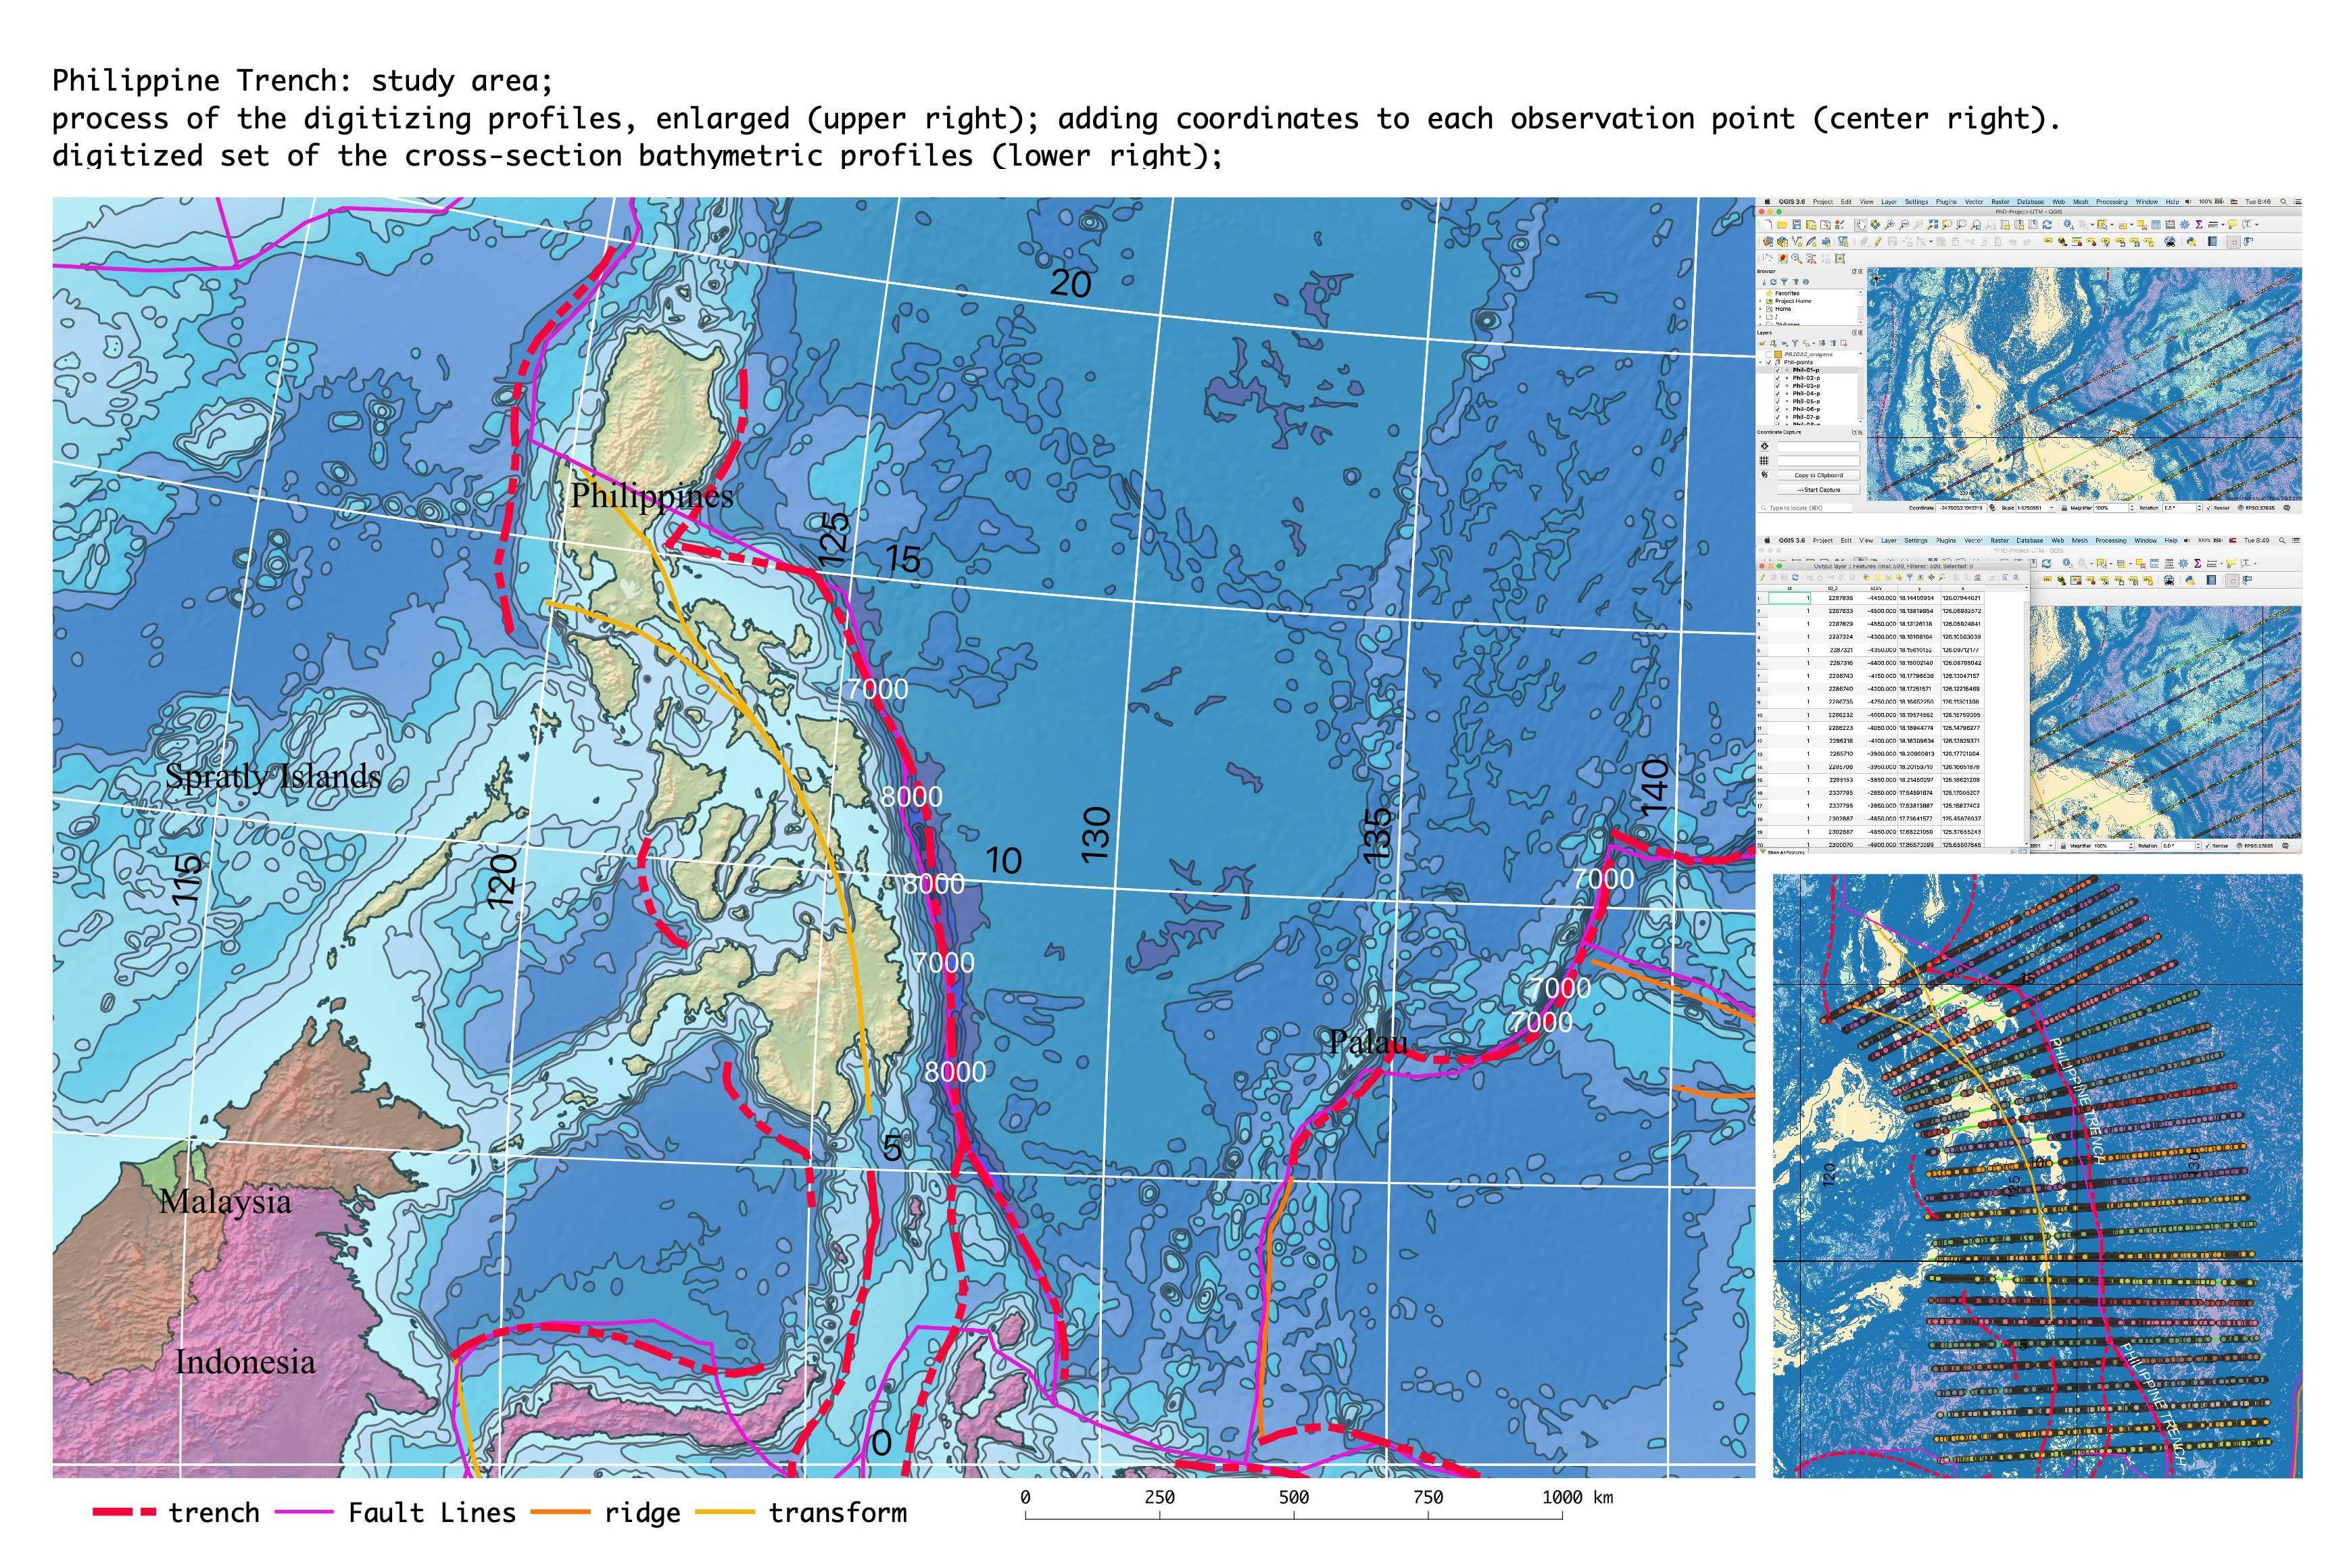
\includegraphics[width=14cm]{Fig-GML1.jpg}
	\caption{Study area and digitizing cross-section profiles of the Philippine Trench and the Philippine archipelago area. Mapping: QGIS}\label{fig:GML1}
\end{figure}

	From the more recent publications on Philippine Trench dynamics it has been noted \cite{Yoshida2017} that fluctuations in the trench dynamics affect slab morphology and character. Another particular feature of the Philippine Trench regions is tectonic plate tearing in the northwestern corner of the subducting Philippine Sea Plate discussed in detailed by \cite{Linetal2013a}.
	\cite{YuChang1991} keep track of the lateral fluctuations in the upper mantle structure of the Philippine Sea basin, which is later more detailed studied by \cite{Yuetal2000} with a more close focus on the geophysics across the Philippine Sea. In some previous case studies \cite{Menard1955}; \cite{Macdonald2001}; \cite{NelsonKulm1973}, using available methods of the oceanographic mapping existing at that time, the geomorphic patterns of the deep-sea channels, submarine fans and their topography were analyzed with regards to the deep-water sedimentation \cite{Divins2003}, mid-ocean ridge tectonics and volcanism, dynamics of the Philippine back arc \cite{Changetal2007}; \cite{Fujiokaetal1999}; \cite{Halletal1995b}, eaqthquakes and gravitation \cite{Lin-Lo2013}. However, given the non available tools of the machine learning and operating with big data in oceanography, those studies significantly lack numerical data analysis and visualization that become possible with the rapid development of the programming algorithms applied in oceanography nowadays. There are proven relationships between the geomorphic structure of the submarine landforms and sedimentation in the selected parts of the Ocean \cite{Dolotov2010}. Other factors include oceanology as underwater currents \cite{Gilleetal2004}, geology \cite{Harrisetal2014}, tectonics \cite{HarrisWhiteway2011}, earthquakes in the Western Philippine Sea Plate\cite{Linetal2013b}, accumulation of the sedimentation that goes into the hadal trenches through the canyon-channel systems \cite{Covault2011}. \\
 	Active usage of numerical computing provided by R and Python enable to widely use statistical methods for marine geological and data modelling. Possible applications include analysis of the interplay between the elements of the submarine ecosystem, predicting possible changes in the structure of the marine ecosystem, reconstruct origin and evolution of the trench dynamics, as well as interpret existing slab motions in the Philippine Plate area, as discussed in many case studies \cite{Sdroliasetal2004}; \cite{Otsuki1990}; \cite{Nakakukietal2008}; \cite{HildeLee1984}. 
	The Philippine Trench is located along the eastern edge of the Philippine archipelago \index[places]{Philippine archipelago}, which is a deformed orogenic belt resulting from the collision of oceanic and continental blocks \cite{Karig1983}. Because of the location in the Philippine and Sunda tectonic slabs collision, the Philippine Fault is proven to have motion in its dynamics \cite{Hiranoetal1986}; \cite{Yu1982}; \cite{Yehetal2013}; \cite{Salahetal2009}; \cite{KatoJordan1999}; \cite{Isseetal2010}. The northwestward motion of the Philippine Sea Plate is partially absorbed by the subduction of first, the Philippine Trench moving westwards, second, the East Luzon Trough  \index[places]{East Luzon Trough} located in the north-east, and third, by the Philippine Fault  \index[places]{Philippine Fault}. Along with geologic factors, tectonic instability of the Philippine Sea Trench necessarily causes variations in the structure of its geomorphology, which is studied in this paper. \\
	The studies of the Philippine Trench included various aspects of the manipulating with data: data search from the web resources, data storage in the \ac{QGIS} platform, geospatial processing, digitizing and geospatial processing using various \ac{GIS} plugins, data capture and export to the csv tables, transfer data sets to R and Python libraries, statistical processing, and finally, modelling and visualizing graphical plots. 

\subsection{Data Analysis}
	The GIS part of this project was performed using \ac{QGIS}, version 3.6.1 Noosa. The study area overview and a \ac{GIS} digitizing workflow are illustrated on the Fig. \ref{fig:GML1}. The stepwise \ac{GIS} part of this research consists of the following steps:
    1. The 1,000 km long profiles were drawn along the trench using ‘Add Line Feature’ tool from the Digitizing Toolbar. 
    2. The intersections between the lines and the bathymetry was done using ‘Vector / Analysis Tools / Lines Intersection’ command. This resulted in the array of the points along each profile. Each point has now a bathymetry depth value and a point reference number.
    3. The latitude and longitude coordinates were then added to the attribute table of each corresponding intersection line using ‘Lat Lon Tools’ plugin of \ac{QGIS}. This plugin was selected since is provided external map support, point digitizing tools, and enables to capture and zoom to coordinates of the profiles.
    4. The coordinates were added to each corresponding profile using plugin function ‘Lat Lon Tools / Conversion / Point layer to fields’. This operation added the initial 25 layer's latitude, longitude (Y, X) to be copied into the text fields in the new layers. Thus, the coordinates were added to the attribute tables. 
    5. The csv files of the attribute tables were exported from the \ac{QGIS} shape files (‘Export / Save Features As’) to csv format for each of the 25 profiles, respectively. 
The topography of the 25 profiles (Fig. \ref{fig:GML2}) was plotted using ‘ProfileFromPoints’ plugin of \ac{QGIS} that enables to plot cross section profile of observation points. Using this plugin the topography data were plotted along a centerline of the cross section profiles using elevation Z (depth values). The resulting profiles are shown on Fig. \ref{fig:GML1}.

The statistical analysis was done using table containing attribute values of the oceanological and geospatial parameters of the Philippine area. The topographic values of the profiles were derived from the table with depth values of all the observation points. The minimal, maximal and quartile values on bathymetry were read into the table. 
	The bathymetric transects Fig. \ref{fig:GML2} were digitized in \ac{QGIS} and their coordinates and attribute values collected as a csv table. Using queries of the \ac{QGIS}, the information on geology of the underlying surface was retrieved (Table 1) to study local geomorphic conditions, variation in the lithology and sedimentation transport processes.  
	The 25 bathymetric transects collected cross-sections of the Philippine Trench and adjacent territories of the Philippine archipelago. Geology and tectonics as attributes were used to analyze their effects on variations in the geomorphology of the trench. Prior to further statistical analyses, we visually inspected the bathymetry cross sections per 25 profiles as shown on the joint facetted plot (Fig. \ref{fig:GML2}). 
	The attribute data were obtained by digitizing cross-sectioning profiles overlaying vector layers on geology, lithology and tectonics. Despite the variations in the density of the observation data points caused by the geomorphic shapes (ranging from extremely steep slope to strong slope), it was possible to merge and integrate the results of the vector overlay. \\
	The statistical part of this research was based on using Python and R statistical libraries that include existing mathematical algorithms and common approaches for the data processing and analysis \cite{DavidNagaraja2003}; \cite{Borradaile2003}; \cite{Cielenetal2016}. The \ac{KDE} analysis (Fig. \ref{fig:GML3}) was carried out using Seaborn library of Python using mathematical algorithms described by \cite{Ciaccioetal2012}. The visualized results of combining five \ac{KDE} plots for the bathymetric cross-section profiles are shown on Fig. \ref{fig:GML3}. It can be seen that combining five profiles enables to compare the geomorphology of the Philippine Trench and significantly increases the recognition of variations and depth and heights from plotting single profiles separately. Thus, the range of the density distribution in the elevations across the Philippine archipelago and Philippine Trench can be seen (Fig. \ref{fig:GML3}). 	
	
\begin{figure}[H]
	\centering
	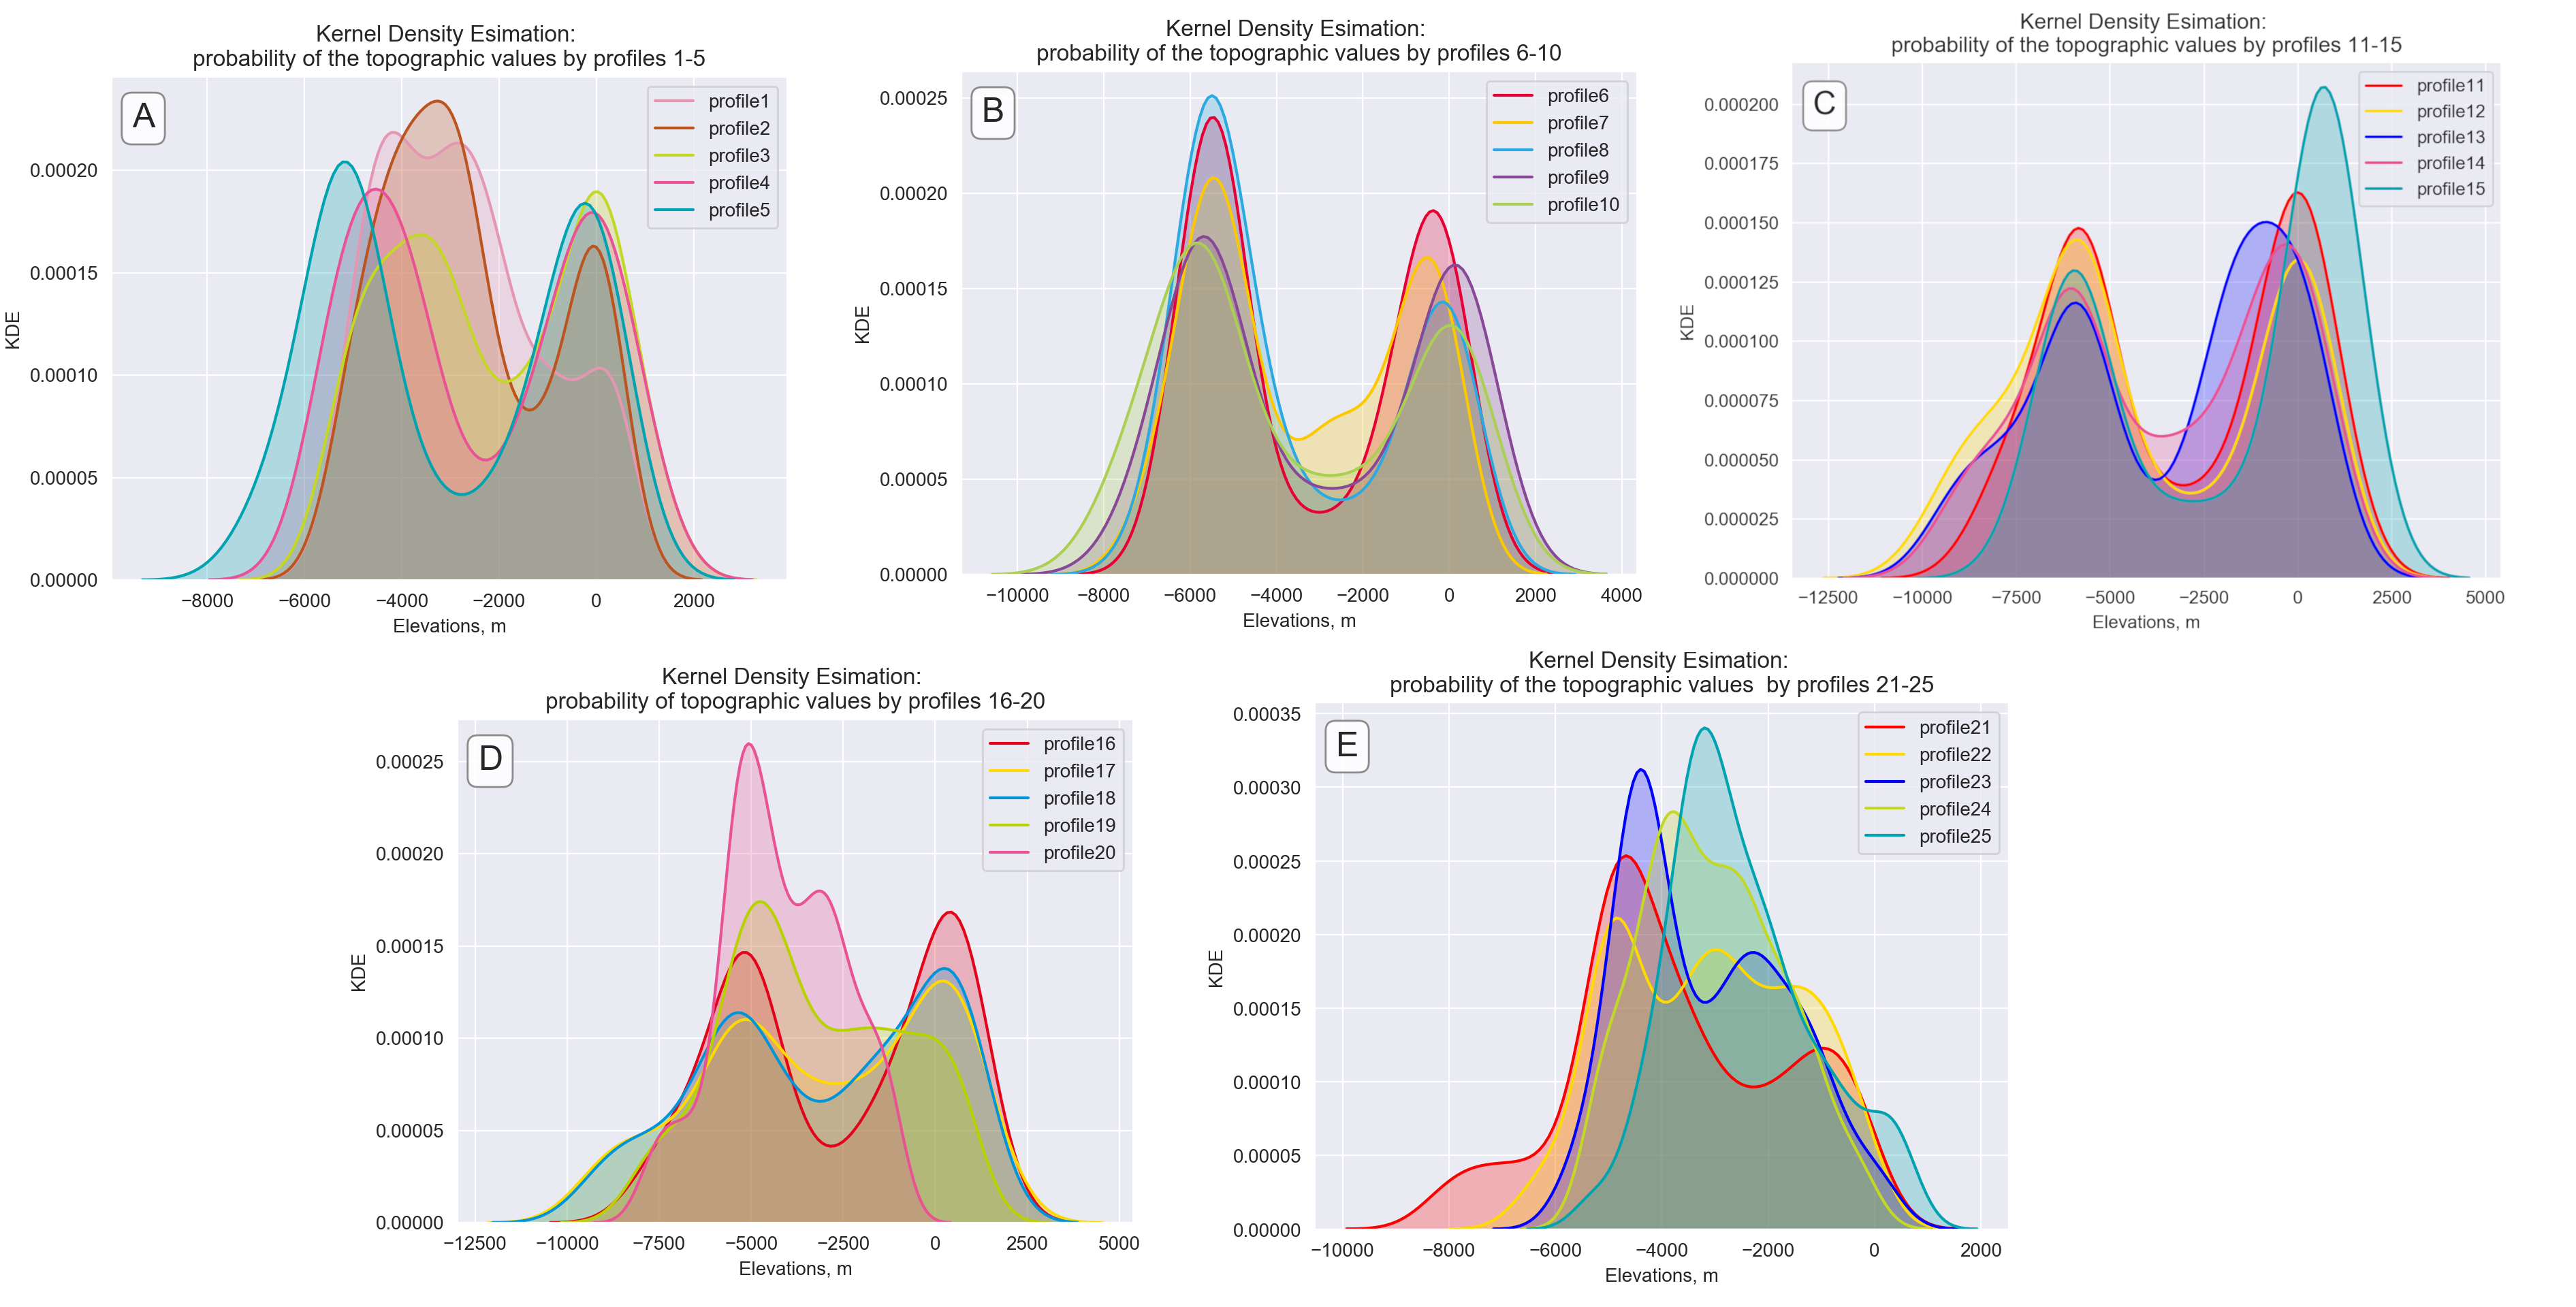
\includegraphics[width=13cm]{Fig-GML3.jpg}
	\caption{KDE plots for the 25 profiles crossing the Philippine Trench area. Plotting: Python}\label{fig:GML3}
\end{figure}

	To better understand the behavior of the spatial distribution in elevations as a stream view, we applied a ridge line technics of the landforms data visualization using functionality of R \cite{RCoreTeam2014}. From the graph showing ridge lines (Fig. \ref{fig:GML4}) one can see the comparative visualization of the density distribution of depths by profiles. Ridgeline profiling provides insight into the statistical distribution of the depth and elevation ranges of the Philippine Trench and archipelago regions. From these profiles (Fig. \ref{fig:GML4}), it is possible to comparatively analyze and observe distribution of an elevation values varied for 25 cross-section profiles. 
	
\begin{figure}[H]
	\centering
	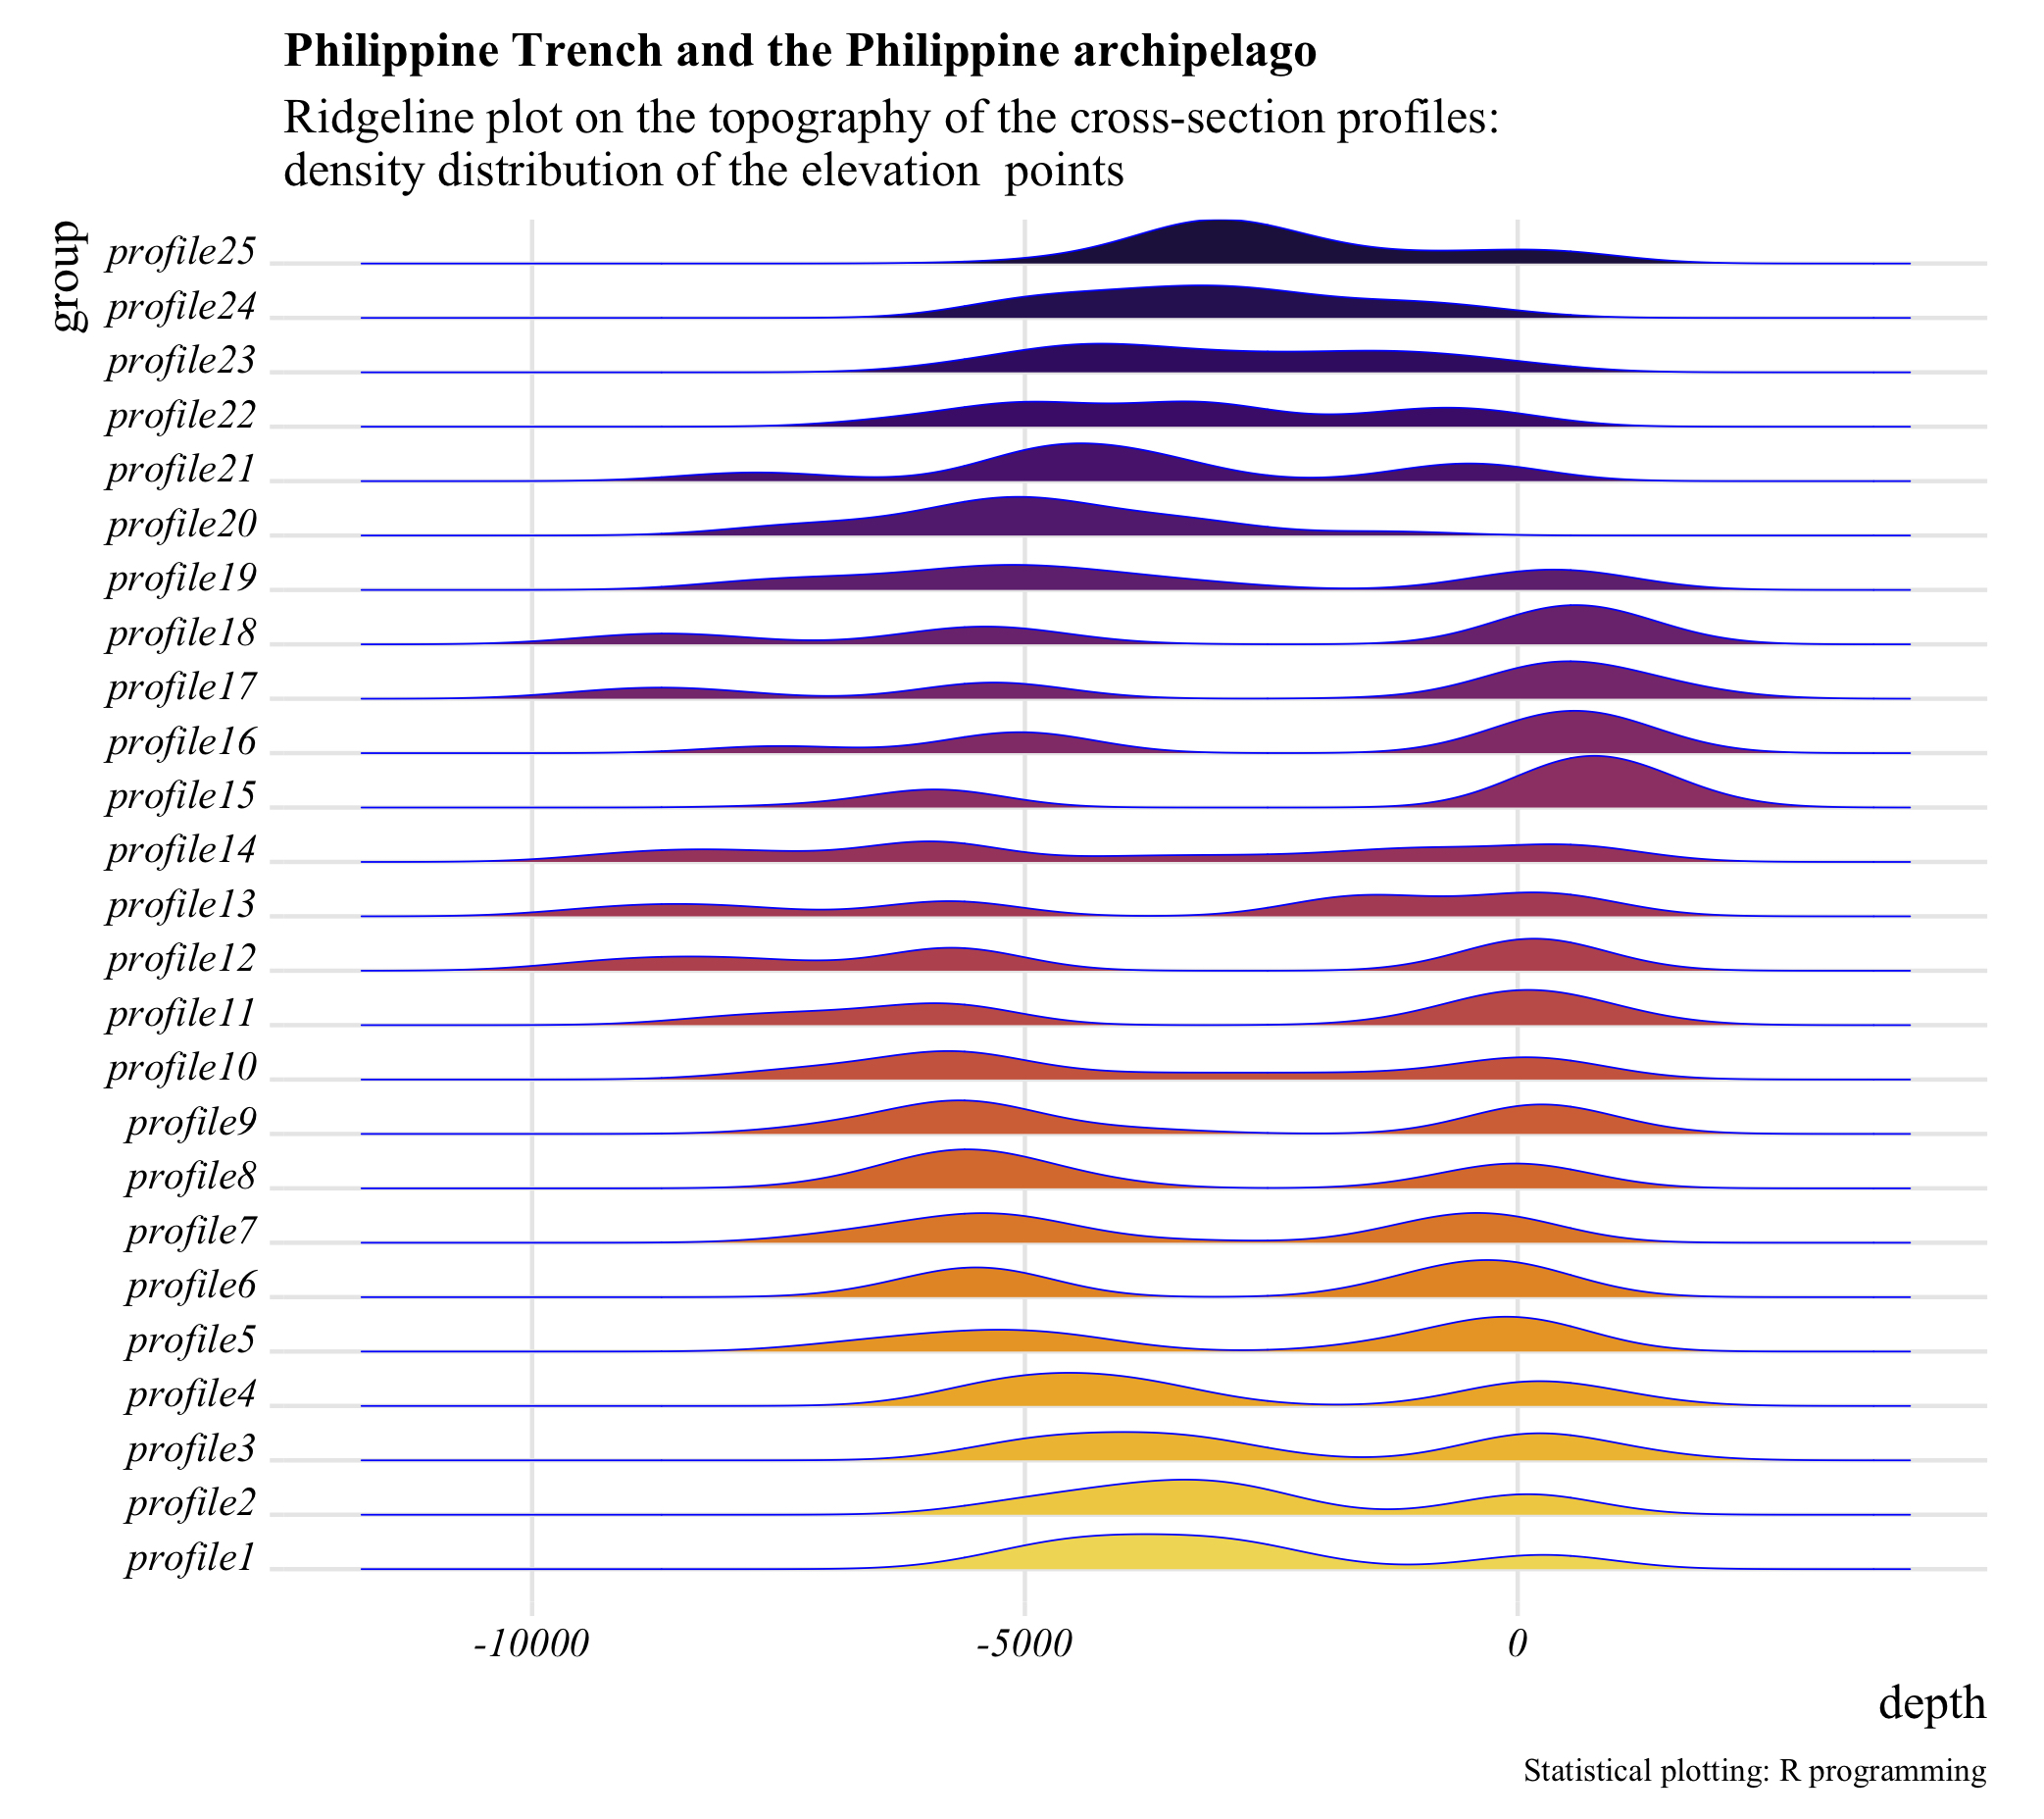
\includegraphics[width=10cm]{Fig-GML4.jpg}
	\caption{Ridgeline plot on the topography of the cross-section profiles, Philippine Trench area and Philippine archipelago. Plotting: R.}\label{fig:GML4}
\end{figure}

	Two elevation curves (Fig. \ref{fig:GML4}) illustrate the ranges across profiles transversal to the main channel of the Philippine Trench and transecting Philippine archipelago, respectively (Fig. \ref{fig:GML5}). For the assessment of the variation in the geomorphology of the trench, it is of significant advantage to visualize the data set using regression analysis (Fig.\ref{fig:GML5}). Regression analysis determines the range, general trend in data distribution and scale of the changes in the observed bathymetry by analyzing changes in the values of the elevation and  (Fig. \ref{fig:GML5}). The following R codes were used for the four methods of the regression analysis visualized on Figure \ref{fig:GML5}: \ref{R:05}. Advantages of plotting a facetted graph consists in visualizing a stream of the data at one look. The algorithms and approaches for the performed regression analysis use existing methods \cite{CameronTrivedi2013}; \cite{Hoaglinetal1983}; \cite{Davis2002} and embedded in \{ggplot\} library of R.
	
\begin{figure}[H]
	\centering
	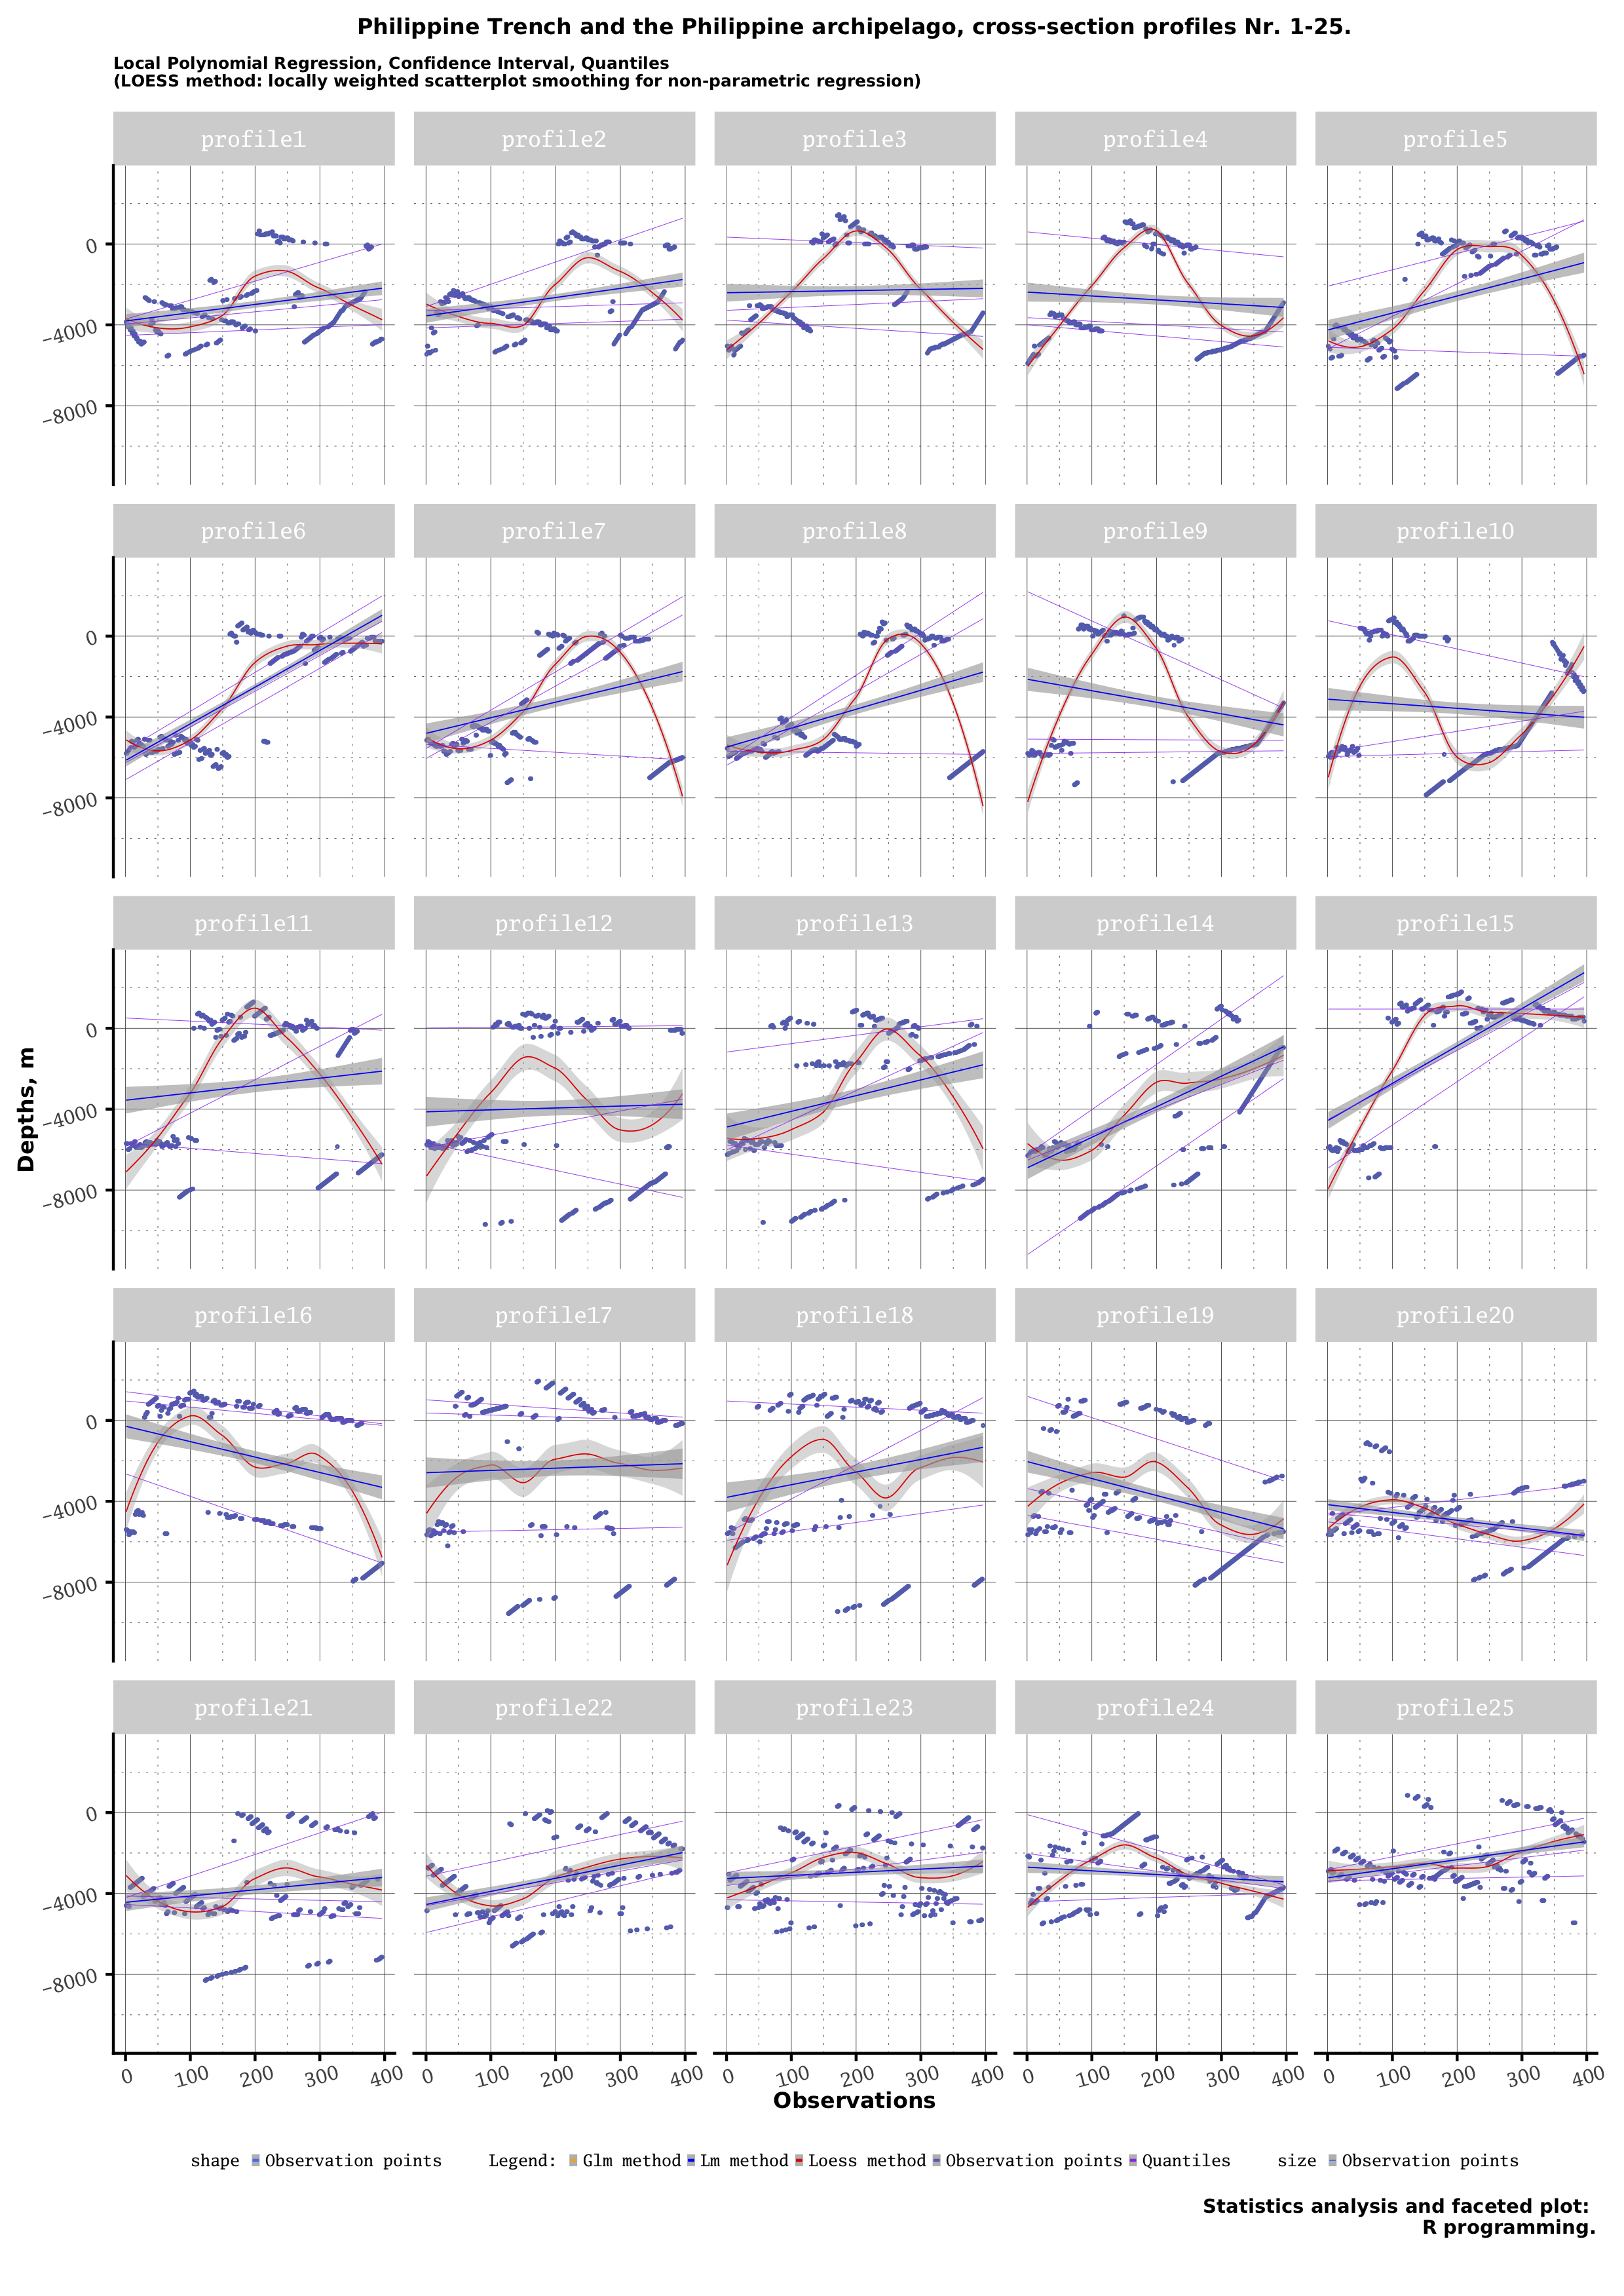
\includegraphics[width=13cm]{Fig-GML5.jpg}
	\caption{Regression analysis plot showing statistical modelling of the cross-section profiles: topography of the Philippine Trench area and Philippine archipelago. Plotting: R by code: \ref{R:05}}\label{fig:GML5}
\end{figure}

	The technical implementation of the letter values plots was based on the existing methods \cite{Hofmannetal2011}; \cite{Hoaglin1983} embedded in modern Python Seaborn library. More sophisticated theoretical explanation on the box plots was given by \cite{McGilletal1978}). Comparing the box plots, the letter value plots are better suited to the oceanographic data sets, since they represent more detailed information in the tails using letter values (Fig. \ref{fig:GML6}) showing statistical data distribution: the samples shown on the letter-value plot illustrate actual range of the bathymetric observations (Y axe) by 25 profiles (X axe). The median, mean and quantiles are shown as horizontal lines on each ‘box’ representing the set of the samples across each of the profile. The plots for the 25 profiles include reliable estimates of their corresponding quantiles (as Tukey’s boxplot) showing outliers (profiles 2 and 3) labeled as observations beyond the most extreme letter values. 
	
\begin{figure}[H]
	\centering
	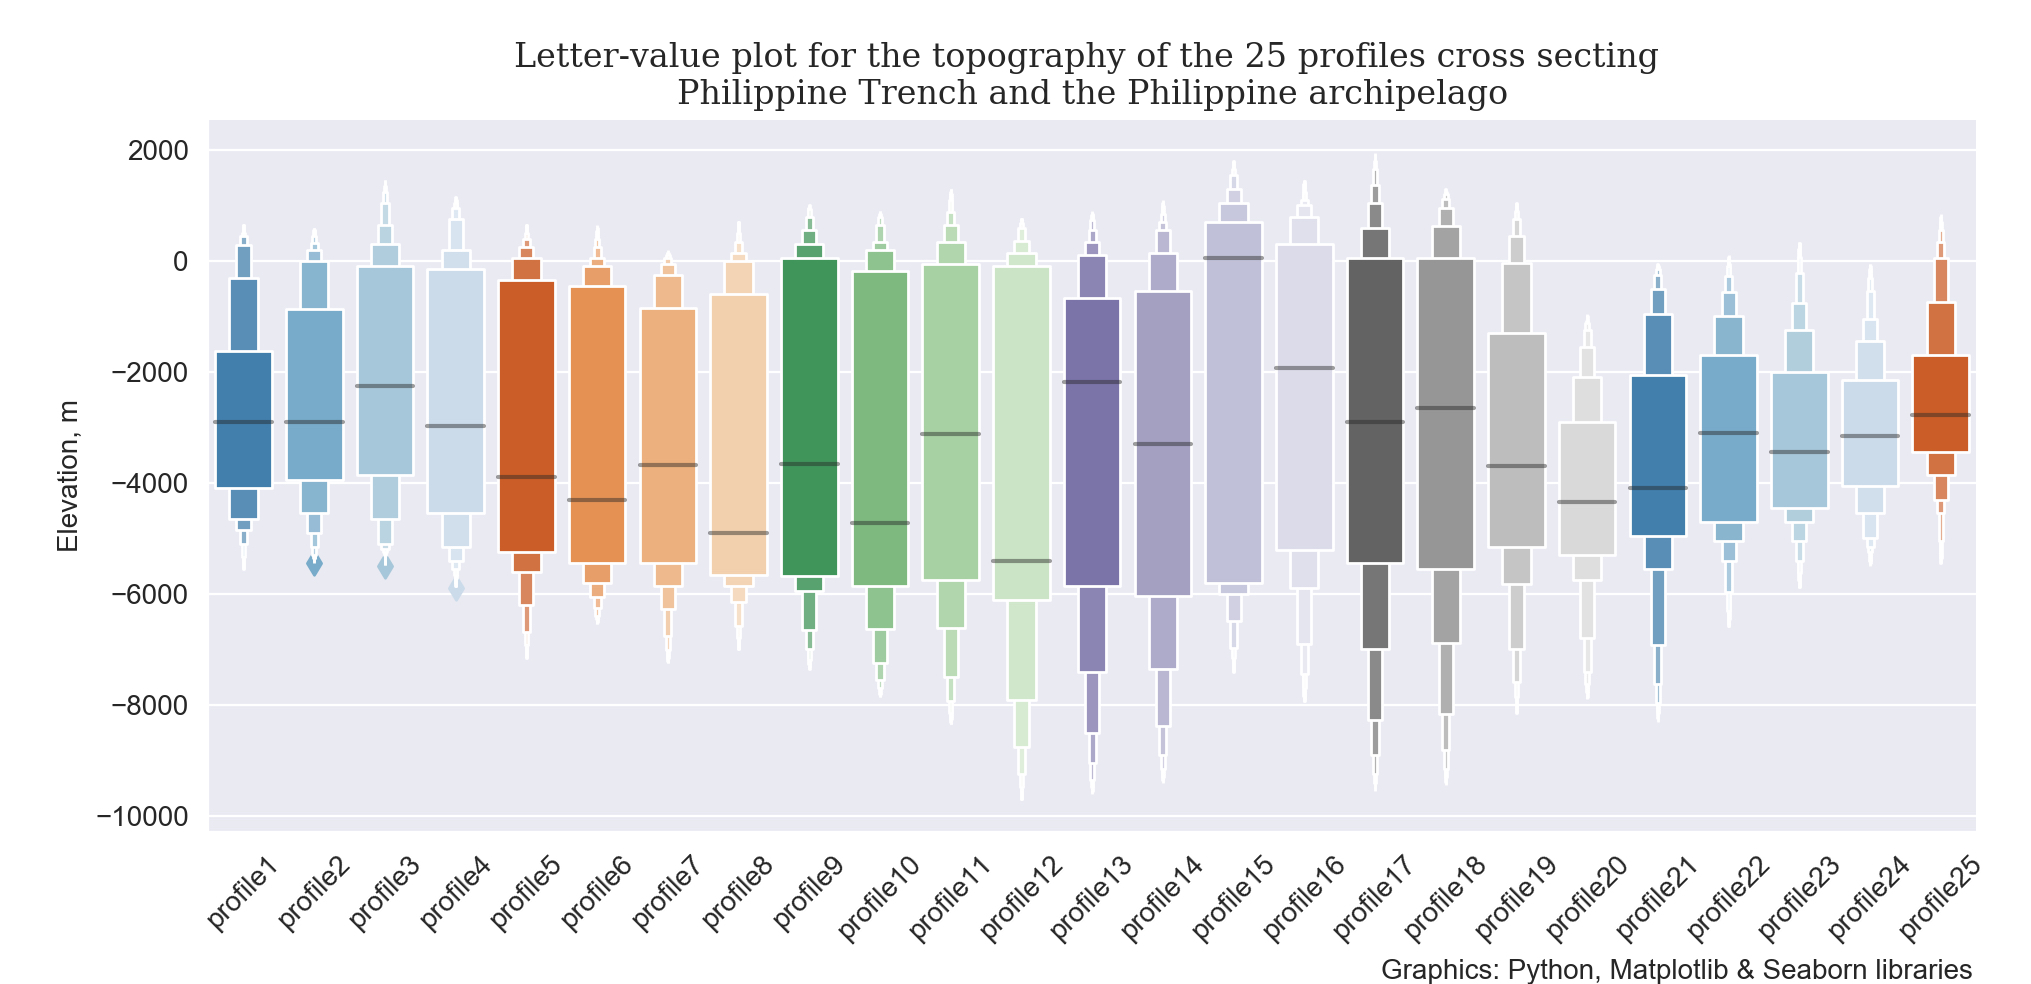
\includegraphics[width=14cm]{Fig-GML6.jpg}
	\caption{Letter-value plot (statistically modified box plot) visualizing descriptive statistics of the topography of the cross-section profiles: mean, median, upper and lower quartiles of the data distribution. Plotting: Python.}\label{fig:GML6}
\end{figure}

	The next part of the research included calculation of the pairwise Pearson correlations and plotting correlation matrix between the geological, geomorphic and bathymetric factors of the Philippine Trench. Methods to plot correlation matrix (Fig. \ref{fig:GML9}) include R based data analysis that embed computing correlograms for the data arrays \cite{GolubVanLoan1996}. The methods and approaches of the Matplotlib and Seaborn libraries used for plotting figures by Python language were derived from the existing literature describing statistical algorithms \cite{Hunteretal2018}. Finally, the geomorphic steepness of the slopes was tested (Fig. \ref{fig:GML10}) using ranking plotting algorithm available in R libraries \{ggsignif\} and \{tidyverse\}. 
	
\pagebreak
	
\section{Manila Trench}

\subsection{Summary}
and interpretation of the topographic profiles, geological sampling, gravity modelling and statistical analysis by means of the \ac{GMT} scripting toolset. A combination of various \ac{GMT} modules was applied for the geospatial modelling aimed at analysis, comparison and visualization of the variations in the geomorphology of the Manila Trench, located in the west Pacific Ocean, South China Sea \index[places]{South China Sea}, west Philippines.

\begin{figure}[H]
	\centering
		\includegraphics[width=15cm]{Fig-M1.jpg}
	\caption{Bathymetric map of the study area based on the SRTM high-resolution 15 sec grid}\label{fig:M1}
\end{figure}

The characterization of the seafloor geology was performed by analyzing the trench and tectonic slabs location as well as areas of the submarine volcanoes. The profile transects were compared and differences in the geomorphic shape in southern and northern parts of the trench were revealed: southern part has steeper slope gradient on the oceanward part; northern part is steeper on the continental slope part. The submarine terraces are located on the northern segment of the trench at depths -2,000 m. The depth and geomorphology of the slope vary for the range -3,500 to -4,500 m: minimals for the northern part of the trench with 526 samples (18,2\%) for the depths -4,000 to -4,200 m. The histogram for the northern part has bimodal distribution with two peaks. The southern part shows 142 values for the minimals - 3,500 to -3400 m. The statistical comparison of the data proved northern part of the trench to be deeper. The \ac{GMT} functionality shown in this paper enabled integration and interpretation of the multi-source data and approaches: automatically digitized profiles, geological mapping, 2D and 3D bathymetric modelling, statistical analysis, mathematical approximation for the trend modelling of the geodata. 

\subsection{Geographic settings}
The Manila Trench \index[places]{Manila Trench} is located in South China Sea \index[places]{South China Sea}, west Pacific Ocean, west of the islands of Luzon \index[places]{Luzon Island} and Mindoro \index[places]{Mindoro Island} in the Philippines (Fig. \ref{fig:M1}). The area of the Manila Trench is located in the Manila subduction zone at the Philippine Sea plate boundary where it moves in the northwest direction toward the Eurasian plate with a high convergence rate \cite{Lo}. The Manila Trench with its maximal depth of the trench about 5,400 m \cite{Liuetal2007} and stretching in almost vertical North-South direction is created by the subduction of the Eurasian Plate (through its part Sunda Plate) under the Philippine Sea Plate. Specific geological structure of the Manila Trench causes potential repetitive earthquakes and seismicity \cite{Wu2009}. Another frequent hazard caused by the subducting slab of the Eurasian plate beneath the Manila trench (Fig. \ref{fig:M7}) is destructive tsunamis causing catastrophic damages in the source area and along the coastlines of the Luzon Island. 

\begin{figure}[H]
	\centering
		\includegraphics[width=13cm]{Fig-M2.jpg}
	\caption{Geologic map of the Manila Trench based on the ETOPO1 1 min grid.}\label{fig:M2}
\end{figure}
The hypocenters of the tsunami of the Manila Trench are located at the depths <100 km \cite{Ruangrassamee}. The tsunami hazard from the Manila Trench source has been assessed in more details in several research papers \cite{Nguyen}, \cite{Bautista}, \cite{Soloviev}. The zone of the Eurasian Plate \index[places]{Eurasian Plate} subduction explains the belt of volcanoes in the Manila Trench area (Fig. \ref{fig:M2}), on the west side of the Philippine island of Luzon \index[places]{Luzon Island}. The area between the northernmost Manila subduction zone and southern Taiwan is considered a transition from subduction to initial collision and a weakly coupled nature for the northern part of the Manila Trench \cite{Chin}. 
\begin{figure}[H]
	\centering
		\includegraphics[width=13cm]{Fig-M3.jpg}
	\caption{Model of the geoid along the Manila Trench.}\label{fig:M3}
\end{figure}
Submarine regions, in contrast with the terrestrial ones, still remain the least accessible areas on the Earth due to their remote location. Therefore, modelling hadal trench is one of the most complicated issues in the marine geology explained by their inaccessibility. Ocean trenches can only be studied using computer based modelling, advanced mapping and algorithms of the data analysis. Therefore, using special software and tools designed for the geospatial data modelling enables to get an insight into the deepest regions of the ocean and to visualize areas with the most difficult access \cite{Calder}. The importance of the seafloor is caused by the uneven distribution of the elevations on the Earth with distinctly uneven hypsography. Thus, the majority of the depths on the Earth is occupied by the deep basins (ca. 4-6.5 km) while relatively few areas are covered by the shallow zones. 
\begin{figure}[H]
	\centering
		\includegraphics[width=13cm]{Fig-M4.jpg}
	\caption{Model of the gravimetry along the of the Manila Trench}\label{fig:M4}
\end{figure}
The tectonic plate boundaries are the hotspot areas where the most of the largest earthquakes take place and oceanic slabs descend beneath the continental lithosphere causing trench migration \cite{Zhangetal2017}. The largest earthquakes mostly occur in the shallow part of the subduction zones \cite{Yu2018}. The earthquakes are sometimes accompanied by strong tsunami waves. Slab dynamics is one of the most important drivers for the trench formation, dynamics and migration. Many factors affect speed and direction of the trench migration. These include plate-mantle coupling, slab interactions with the mantle transition, plate geometry, kinematics, strain rate, temperature, fluid pressure, deformation mechanisms, as well as mantle rheology \cite{Faccennaetal2018}. \\
The geological complexity of the Manila Trench is also expressed by the connection with the Philippine Trench where a horizontal mantle flow exists between the Manila Trench and the Philippine Trench. It is caused by the collision between the Palawan block and the Philippine Mobile Belt, and movement off the South China Sea \index[places]{South China Sea} slab \cite{Fan}. Various factors cause the formation of the Manila Trench. Being a hadal trench, it presents a special area of the ocean seafloor with distinct geomorphological structures characterized by the notable depths and steep gradient angles, located in the zones of the continental margin tectonic plates bending. The convergence between the two plates forming the Manila Trench is roughly northwestward. There is a high-velocity zone present in the crust and upper mantle beneath the Luzon Arc \index[places]{Luzon Arc} where the Manila Trench is stretching \cite{Doo2016}. All these factors briefly mentioned to illustrate the tectonic settings of the study area indicate high seismicity and special tectonic zone where the Manila Trench has been formed. The seafloor of the hadal trench presents a complex structure combined of of various landforms: mid-ocean ridges, transform faults, ocean plains complicated by chains of seamounts, minor ridges, trenches and plateaus. 
\begin{figure}[H]
	\centering
		\includegraphics[width=13cm]{Fig-M5.jpg}
	\caption{3D map of the Manila Trench visualizing geomorphology}\label{fig:M5}
\end{figure}
Factors influencing geomorphic development, structure and bathymetric patterns of the trench are diverse. To mention some of them: geological, hydro-chemical, geothermal, climatic, tectonic and bathymetric determinants. The steepness of the Manila geomorphology varies: the dip angles along the Manila Trench \index[places]{Manila Trench} increasing gradually southwards from ca. 25\degree at the latitudes between 18\degree and 21\degree N, 32\degree at the latitude 17\degree N, and nearly vertical at the latitude 14\degree N \cite{Chengetal2019}. The tectonic front of the Manila Trench continuing northward into the frontal thrust faults in the western Taiwan shows active plate boundary between the Eurasian and Philippine Sea plates in the Luzon-Taiwan region \cite{Yu2004}. The structure of the northern Manila Trench has been studied in various papers focused on the problems of crustal structure and deformation in the north of the Manila Trench \cite{Lietal2013}, \cite{He2016}, \cite{Ku2009}. Among other findings, the increasing dip angle of the Manila Trench from north to south has been discovered. The Manila Trench loses its sharp bathymetric pattern in the early collision zone and gradually becomes a less well-defined deformation front \cite{Lester2013}. However, the comparative analysis of its southern and northern parts is still missing. Therefore, current paper contributes to better understanding of the Manila Trench by comparative analysis of its geomorphology in the northern and southern segments.

\pagebreak
\section{Ryukyu Trench}
The \index[places]{Ryukyu Trench} is a 1400 km long hadal oceanic trench, stretching along the southeastern edge of the Ryukyu Islands Arc \index[places]{Ryukyu Islands Arc}, between the Philippine Sea, Taiwan Island \index[places]{Taiwan Island} and Kyushu Island \index[places]{Kyushu Island}, southern Japan \index[places]{Japan}, Pacific Ocean \cite{Ando} (Fig. \ref{fig:R1}). The trench was formed as a result of the subduction of the oceanic crust of the Philippine Sea Plate beneath the continental crust of the Eurasian Plate \index[places]{Eurasian Plate} \cite{Doo}. The aim of the research is to analyze differences in the geomorphology and bathymetry of the northern and southern parts of the trench using \ac{GMT} \cite{Wesseletal2013}.

\begin{figure}[H]
	\centering
		\includegraphics[width=13cm]{Fig-R1.jpg}
	\caption{Bathymetric map of the East China Sea, northern Philippine Sea, Ryukyu Arc and Ryukyu Trench. The bathymetry is based on GEBCO mapped using GMT.}\label{fig:R1}
\end{figure}

The bathymetric pattern of the Ryukyu Trench varies in its northern and southern parts which reflects the correlation between the geomorphic shape of the hadal trench, steepness of its gradient slope angles and tectonic settings in the area. Thus, in the northern part of the trench, the subduction of the Philippine Sea Plate is notable for shallow depths and steepness, reaching only ca. 11\degree. On the contrary, the angle becomes steeper, reaching 70\degree below ca. 70 km. The region located to north-west of the Ryukyu Volcanic Arc \index[places]{Ryukyu Volcanic Arc} is a \ac{BAB}, a depression of the Okinawa Trough \index[places]{Okinawa Trough} (Fig. \ref{fig:R2}).

\subsection{Tectonics}
The subduction of the Philippine Sea tectonic plate causes eruption of the approximate 34 volcanoes (Fig. \ref{fig:R2}) and earthquakes producing tsunami. In contrast, the slab dip in the central and southern parts of the Ryukyu trench is more gentle, reaching 40-50\degree at 70 km depth \cite{Kodaira} \cite{Long}. There are three groups of islands on the forearc basement stretching over the Ryukyu arc \cite{Kizaki}. The Kerama Fault \index[places]{Kerama Fault}, about 250 km wide (Fig. \ref{fig:R2}), separates the southern from the central group of islands.

\begin{figure}[H]
	\centering
		\includegraphics[width=13cm]{Fig-R2.jpg}
	\caption{Geologic map of the Ryukyu Trench based on ETOPO1, GMT}\label{fig:R2}
\end{figure}

The Ryukyu Trench reaches depths of 7000 m \ac{BSL} and the forearc slope between the forearc island chain and the trench is between 130 to 160 km wide. The northern group has Yaku-shima \index[places]{Yaku-shima} and Tanega-shima \index[places]{Tanega-shima} and a 200 km long Tokara Channel \index[places]{Tokara Channel} gap between the island groups \cite{Okamura}. The tectonics of the hadal trench reflects evolutional processes of the building seamounts and the structure of the Earth’s crust. Therefore, it causes variations in the lithological patters, geological conditions of the rocks formation, stratigraphy and sedimentary settings of the ocean seafloor formation during Jurassic, Mesozoic and Cretaceous. Double subduction system of the Ryukyu Trench reflects the complex trench motions as an expression of the interaction between the subducting plates and the underlying mantle of the Ryukyu Trench. The Pacific plates subducts beneath the Philippine Sea Plate, which is in turn subducting beneath the Eurasian Plate along the Ryukyu Trench \cite{Faccennaetal2018}.

\subsection{Geomorphology}
Geomorphology of the ocean seafloor results from the complex geodynamic processes. These demonstrate traces of the continuous evolution and shape seabed surface as a system of the mid-ocean ridges, transform faults, vast ocean plains complicated by chains groups, ridges and plateaus as well as minor forms such as terraces, seamounts and hills, Fig. \ref{fig:R5}. Various factors affect the trench geomorphology and in turn, are reflected in its complex structure and functionality of the submarine environment. To mention some of them: effects of the magmatism \cite{Kiminami}, seismicity \cite{Theunissen}, \cite{Gutscher}, volcanism and hydrothermal system \cite{Minami2018}, \cite{Minami2016}.

\begin{figure}[H]
	\centering
		\includegraphics[width=13cm]{Fig-R3.jpg}
	\caption{Model of the geoid in the Ryukyu Trench area}\label{fig:R3}
\end{figure}

Another example is the effect of the thickness of the subduction channels and earthquake rupture segments on the geomorphology of the oceanic landforms. Thus, the spatial differences of the Ryukyu Trench geomorphology is reflected in its sediment composition that change systematically from lighter off northern Ryukyu arc to heavier along the central part of the Ryukyu arc. This is explained by the dominance of the terrigenous and pelagic sedimentation off of the northern and central Ryukyu arc, respectively \cite{Shu}.

\subsection{Sedimentation}
The hadal trench presents a structural trap in the continental margins of the Pacific since the sediments are carried by the ocean currents passing through the system of trenches on the west of the Pacific. The sediment types of the Ryukyu Trench include among others mud diapirs, hemipelagic sediments, mud-supported breccia, fossil planktonic foraminifera, calcareous nannofossils \cite{Ujiie}.
The content of the planktonic foraminifera varies according to the seasonal warming of surface waters and vertical mix as a result of the NW monsoon \cite{Xu}. Seismic investigations of the Ryukyu Trench area show that the sedimentary thickness is ca. 2-3 km on the oceanic plate, oceanic crust thickness is 5-6 km. The upper mantle material underlying the oceanic plate has low seismic velocities, explained by the geochemical processes of the mantle peridotites \cite{Klingelhoefer}.

\begin{figure}[H]
	\centering
		\includegraphics[width=13cm]{Fig-R4.jpg}
	\caption{Model of the gravitational settings in the Ryukyu area.}\label{fig:R4}
\end{figure}
Submarine margins of the continents can be divided into two types: the passive and active ones, depending on the features of the geomorphology and geology. The active margin in the Ryukyu area is located off northern Taiwan in the southern Ryukyu forearc (Fig. \ref{fig:R2}). A mega-splay fault system associated with great earthquakes in the south of the Ryukyu region is described by \cite{Hsu}. Indeed, the southwestern Ryukyu system is characterized by the edge regime that is heavily influenced by the juxtaposing continental lithosphere \cite{Kuo}.

\subsection{Marine biology}
Although the seafloors of the Ryukyu trench is separated vertically from the euphotic zone, is serves as a depositional center for the organic carbon accumulation. This is caused by the geomorphological factors: steep slopes enable lateral transport from the adjacent continental margins \cite{Itohetal2011}. Studies on the spatial biodiversity of the Ryukyu Trench show \cite{Kitahashietal2014b} low values at shallow depths, but increased with water depth reaching maximum between the trench floors and abyssal plains. This proves that bathymetric patterns of the deep-sea biomass of the Ryukyu Trench spatially differ in various regions of the trench. 

\begin{figure}[H]
	\centering
		\includegraphics[width=13cm]{Fig-R5.jpg}
	\caption{3-D mesh geomorphological modelling of the Ryukyu Trench}\label{fig:R5}
\end{figure}

Such discrepancies reflect differences in the environmental conditions, e.g. primary productivity. level. This is also supported by the discoveries of the migration patterns in the Ryukyu Trench area where reefs and geomorphic landforms serves as a land bridge for the migration of terrestrial organisms from Okinawa-jima to Miyako-jima \cite{Arai}.


\subsection{Conclusion}
This work offers an overview of geomorphological situation conducted using \ac{GMT} based modelling and cartographic mapping. The research aimed at analyzing differences in two selected segments located in southern and northern parts southwards the Miyako Fault \index[places]{Miyako Fault}. The study presents a multidisciplinary approach combining cartographic modelling and marine geological analysis. The results obtained enabled to detect variations in the slope angle of the trench that shows more steep gradients and deeper bathymetric values in the northern segment and shallower depths with more gentle slope in the southern, respectively.
Technically, an experimental approach of the cartographic modelling combined with numerical statistical analysis (modeled trends and histograms) using \ac{GMT} modules was used to analyze geological and geophysical data sets. Cartographic visualization of the series of thematic maps (geology, bathymetry, geoid, gravimetry, 3D modelling, 2D profiles trends modelling, digitized cross-section profiles) demonstrated powerful functionality of the \ac{GMT} and proved it to be effective cartographic instrument for the data analysis. The increasing diversity of the spatially distributed data on the Earth observation together with application of the advanced cartographic methods and scripting tools greatly enhance the potential of the geospatial modeling.
 Application of the cartographic modelling towards marine geological data enables to detect spatial differences in the submarine geomorphology that can only be studied using modelling tools due to their remote location. In turn, modelling spatial variations of the trench geomorphology helps to highlight dynamics of the plate tectonics and facilitates our understanding of the ocean seafloor geomorphology.

\pagebreak
\section{Palau Trench}

\pagebreak
\section{Yap Trench}
The Yap Trench \index[places]{Yap Trench} is located \\
Watermass properties and deep currents in the northern Yap Trench were observed and discussed recently by \cite{Liuetal2018a}.

\pagebreak
\section{Mariana Trench}
\subsection{Geographic location}
\subsubsection{Bathymetry}
Mariana Trench \index[places]{Mariana Trench} is a long and narrow topographic depression of the sea floor, located in the west Pacific Ocean \index[places]{Pacific Ocean}, 200 km to the east of the Mariana Islands, eastwards of the Philippine Islands \index[places]{Philippine Islands} and China \index[places]{China}, Fig. \ref{fig:BathyMT}. It belongs to the deepest trenches of the Earth, with maximal depths above 9-11 km, all of which are located in the western half of the Pacific Ocean.

\begin{figure}[H]
	\centering
	\includegraphics[width=14cm]{Bathy-MT.jpg}
	\caption{Mariana Trench. Mapping: GMT}\label{fig:BathyMT}
\end{figure}

It is the deepest part of the World Ocean \index[places]{World Ocean} with a maximal depth of 10,984$\pm$ 25 m (95\%) at 11.329903\degree N / 142.199305\degree E m at the Challenger Deep\index[places]{Challenger Deep} \cite{Gardneretal2014}. North-western Pacific Ocean is especially characteristic for the vast areas of the bottom of the basins occupied by depressions deeper 6000m with a special case of Mariana Trench. Despite the extreme bathymetric values of the Mariana Trench at Challenger Deep, its structure has following pattern: a major total area is being occupied by the abyssal depths (3-6 km), while the extreme depths exceeding 6 km, are smaller in comparison to the previous areas \cite{UyedaKanamori1979}. The abyssal make up relatively small part of the total area of the Mariana Trench, while the second ones cover about two thirds of the whole. Depths of more than 6000 m are confined mainly to the deepest part of the trench located in the south-western part of the Mariana Trench, although individual depressions to depths of 6-7 km, rarely up to 7.5 km, occur in the central part of the basins along the trench \cite{Morgan1974}. The typical depths of the ocean floor of the Mariana Trench are 4000-5000 m where mid-ocean ridges and deep-sea basins formed by numerous seamounts \index[concepts]{seamounts} and deep-sea depressions\index[concepts]{deep-sea depressions} are located. \\
The general form of the bathymetric structure of the Mariana Trench is inclined toward the margin plate being connected with the ocean basic zone. It has high and steep island or continental slopes and more low and gentle slopes from the south-eastern side. The main area of the seafloor of the trench has prevailing depths of more than 3000 m, a seabed being the most ancient parts of the ocean floor formed in the late Jurassic \index[concepts]{Jurassic}.
The geographic location of the edge of the Mariana Trench along the coasts of the continents or island arcs is explained mainly by the subduction of oceanic tectonic plates at the boundaries of their collision with Mariana \index[places]{Mariana Plate}, Pacific \index[places]{Pacific Plate}, Philippine \index[places]{Philippine Plate}, Caroline \index[places]{Caroline Plate} tectonic plates \ref{Ishibashietal2015}. The seabed structure of the Mariana Trench is composed in the following way from top to bottom: a sedimentary cover, a basalt of the leitic composition, a complex of parallel dykes of diabases \index[concepts]{diabases}, an isotropic gabbro\index[concepts]{gabbro}, a banded gabbro-ultrabasic complex \index[concepts]{gabbro-ultrabasic complex} lying on the mantle \index[concepts]{mantle} ultrabasites\index[concepts]{ultrabasites} \ref{Butuzova2003}. There are differences in the velocity of the longitudinal seismic waves in the geological layers of the Mariana Trench structure: water and sedimentary layer have speed of 3.5 6.2 km/s, basalt\index[concepts]{basalt} layer has speed of 6.5-7.0 km/s. The layer of gabbro and banded gabbro are located beneath. The boundary of the crust-mantle \index[concepts]{crust-mantle} is made by a sharp increase in the velocities from 7 to 8 km/s (the boundary of the Mohorovicic). The upper mantle is the region with the velocities of 8.0-8.2 km/s \cite{Garfunkeletal1986}. Analogues of the oceanic crust on the ground are ophiolites \index[concepts]{ophiolites}. The average thickness of the crust of this type under the platforms is about 40 km \cite{Gurevich1998}. The regions with bark continental type in the ocean are fragments of continental mass formed as a result of the formation of the modern ocean floor \index[concepts]{ocean floor} causing migration and slow movement of the trench \cite{Husson2012}.

Mariana Trench has a a distinctive morphological feature of the convergent plate boundaries, along which lithospheric plates \index[concepts]{lithospheric plates} move towards each other, located about 200 km parallel to a volcanic island arc \index[concepts]{volcanic island arc} \cite{Karatoetal2001}. The formation of the trench is caused by the complex interconnection of various environmental factors \cite{Gardneretal2014}. A trench marks the position at which the subducting slab \index[concepts]{subducting slab} descends beneath another lithospheric slab \cite{DeschampsLallemand2003}. Mariana Trench presents a strongly elongated, arched in plan and lesser rectilinear depression stretching for hundreds kilometers and having a narrow depression on the ocean floor with very steep slopes \index[concepts]{slopes} and the depths of 3-5 km width of the bottoms rarely exceeding 5 km in breadth \cite{NakanishiHashimoto2011}. Mariana Trench has complicated steps of various shapes and sizes, caused by active tectonic and processes of sedimentation \index[concepts]{sedimentation}. The steepness of its geomorphic depth averages in 4-5 \degree, but its individual parts can be limited to steeper slopes as subjects to the gravitational flow system \index[concepts]{gravitational flow system} of the submarine canyons \index[concepts]{submarine canyons} and valleys \index[concepts]{submarine valleys}\cite{Kawabe1993}. Complex distribution of the various geomorphic material on the adjacent abyssal plains \index[concepts]{abyssal plains} of the ocean contributes to the formation of the geomorphic features of the particular region of the Mariana Trench.

		\subsubsection{Geometry and Shape}
Mariana Trench has a distinctive morphological feature of the convergent Pacific plate boundaries, along which lithospheric plates move towards each other. Mariana Trench presents a strongly elongated, arched in plan and lesser rectilinear depression. Its transverse profile is asymmetric: the slope is higher on the side of the Mariana island arc \index[places]{Mariana Arc}. The slopes of the trench are dissected by deep underwater canyons. Various narrow steps are also often found on the slopes of the trench. On the longitudinal profiles of the bottom of the Mariana there are many deepwater detected transverse steps and thresholds \index[concepts]{thresholds} connected by the movements of the earth's crust along transverse faults\index[concepts]{faults} \cite{Zhouetal2015}. These thresholds can play important role in the evolution of the deep water trough \index[concepts]{trough}, for example, to control the intensity of its filling by sediment precipitation \index[concepts]{sediment precipitation}. In this process very important are the streams of the precipitation moving along the bottom from the part of the trough which is closer to the continent \cite{Tairaetal2004}. At the bottom of the trough there is a transverse threshold, which can present kind of a dam, in front of which there is accumulation of a thick layer of sediment precipitation.\\
The total length of the trench measures about 2,550 km long approximately. Mariana Trench is one of the 37 known deep-water trenches of the World Ocean, 28 of which located in the margin areas of the tectonic plates of the Pacific Ocean \cite{PushharovskijNeprochnov1984}. It forms the peripheral framing, of which five are located in the  \index[places]{Atlantic Ocean} Atlantic Ocean \cite{Bogdanov1997} and four in Indian Ocean \index[places]{Indian Ocean} \cite{Gurevich1998}. Crossing four tectonic plates – Mariana, Caroline, Pacific and Philippine, – Mariana Trench creates a complex of the deeply interrelated factors and processes. Factors affecting formation, geomorphic development and bathymetric patterns of the Mariana Trench are diverse. The most important ones include geological, hydro-chemical, biological, geothermal, climatic, tectonic, bathymetric and geomorphological determinants. For instance, the impact of lithosphere \index[concepts]{lithosphere} is illustrated by a constant exchange of matter and energy between the submarine volcanoes \index[concepts]{submarine volcanoes} located nearby \cite{HussongUyeda1982}. The hydrosphere \index[concepts]{hydrosphere} influence on the Mariana Trench is reflected by deep ocean currents bringing sediments to the trench bottom and contributing towards accumulation of the sediment thickness \cite{HorlestonHelffrich2012}.

	\subsection{Geology}
		\subsubsection{Sedimentation}
Thin Quaternary \index[concepts]{Quaternary, period} clayey sediments overlie a 400 m thick alternating sequence of the Early Cretaceous \index[concepts]{Cretaceous, Early} quartz-trachyte \index[concepts]{quartz-trachyte} pillow lava and Early to Late Cretaceous \index[concepts]{Cretaceouse, Late} radiolarian cherts in the oceanward slope of the Mariana Trench \cite{Hiranoetal2002}. The sediment cover is less than 10 m thick and is composed of soft, bedded clay with sand-size ash fragments. This clayey sediment covers a very gentle terrace 500 m wide \cite{CurtisMoyer2005}. The turbidite currents \index[concepts]{turbidite currents} are being generated on the outer shelf and upper continental slope \index[concepts]{continental slope}, due to the precipitation and transport via the submarine canyons to the axial part of the trench. The speed of such sedimentation in the bottoms of trenches closely depends on the volumes of the incoming sediments \index[concepts]{sediments} ranging from 300 to 3000 mm/thousand years \cite{Ishizukaetal2018}. 
As a result of such sedimentation, over one kilometer of sediments have accumulated in the southern Aleutian \index[places]{Aleutian Trench} and Peru-Chile trenches \index[places]{Peru-Chile Trench} over the last several hundred thousand years. On the bottom of the deep ocean trenches a longitudinal main channel is usually formed under the influence of turbidite currents \cite{Pabstetal2012}. It creates favorable conditions for distinctive movements of the sand sediments that shape large elongated accumulations of the sediments \cite{Ernst2001}. As a hadal trench, Mariana Trench belongs to the one of the deepest 45\% of the ocean’s depth range, and its unique topography disrupts the continental shelf- slope-rise to abyssal plain continuum, resulting in an array of deep isolated habitats. The often abrupt and distinct topography is likely to further promote speciation through high hydrostatic pressure, remoteness from surface derived food sources and geographic isolation \cite{Eustaceetal2016}. \\
Processes of the deep-sea terrigenous sedimentation are formed by the transfer of the erosion materials from the adjacent land. The main processes include transportation, deposition and re-deposition of the sedimentation materials. The origin of the deep ocean sedimentation is diverse. In general, apart from the sediments from the rivers, the terrigenous material goes to the oceans through iceberg melting and glacial deposits transferred to the seafloor, as well as dusty material moved by the aeolian processes. Normally, the sediments transferred by rivers are deposited within the shelf sublittoral areas, and rarely reach deeper regions of the continental slope and, even less the abyssal basins. However, sediments deposited on the shelf may move to the deeper parts of the ocean including hadal trenches, due to further move from the shelf edge downwards, avalanche sedimentation, i.e. gravitational flows, which are caused by the gravity. For the case of the Mariana Trench, the deep currents flow through the trench ventilating its bottom water flowing through the West Pacific trenches originates from the Southern Ocean \index[places]{Southern Ocean} and Antarctic \index[places]{Antarctic} and flows northward \cite{Warrenetal1988}, in a clockwise direction, passing through the trenches on the west of the Pacific (i.e. the Kermadec Trench and the Tonga Trench. Through the Samoan Passage, it flows northwest across the equator to the east Mariana Trench. Among other hadal trenches \index[concepts]{hadal trenches}, Mariana Trench is the largest structural trap located in the continental margins \index[concepts]{continental margins}. Therefore, the geomorphic conditions of Mariana Trench create ideal conditions for the sedimentation processes intercepting almost all clastic material \index[concepts]{clastic material} originating from the adjacent land. The accumulation \index[concepts]{sedimentation, accumulation} of the terrigenous sedimentation \index[concepts]{sedimentation, terrigenous} on the Mariana Trench seafloor depends on various factors. These include climatic and hydrodynamic local characteristics, tectonics, structure of the seafloor bathymetry, geomorphic characteristics of the trench, type and size of particles and others. Large areas of active sedimentation processes can be distinguished in the areas where the speed of the sedimentation and their volumes are very high, as well as local areas of active sedimentation, or, on the contrary, dominating erosion areas. In general, sedimentation processes mainly occur in various sediment traps, however, some areas are noted by areal sedimentation. Therefore, the processes of the sedimentation within the Mariana Trench are highly uneven.

\subsubsection{Lithology}
The lithological structure and sediment thickness are among the other factors affecting Mariana Trench formation. Relatively few other trenches, comparing to Mariana Trench, also formed on the boundaries of the tectonic plates, but usually at a greater distance from the continents in the rift zones \index[concepts]{rift zones}. Therefore, the sedimentation processes within Marina Trench are deeply impacted by the location near the rift zones that are mainly associated with the formation of the underwater mountain ranges \index[concepts]{underwater mountain ranges} and spreading \index[concepts]{spreading}. Their expansion in the sides of the neighboring lithospheric plates is a result of the rise towards Mariana Trench. The outflow to the surface of the ocean floor of the substance of the upper layer of the Earth's mantle \index[concepts]{Earth's mantle}. As a result of the unevenness of this process, the transversed faults are formed that have excellent conditions for sedimentation accumulation. According to available geophysical data \cite{DubininUshakov2001}, the oceanic crust of the tectonic plates surrounding Mariana Trench is composed by a number of layers. Therefore, the impact of the sediment subduction \index[concepts]{subduction} on the trench dynamics \index[concepts]{trench dynamics} is relatively high, which is highlighted by \cite{HorlestonHelffrich2012}.

	\subsubsection{Geomorphology}
	\paragraph{Geomorphic structure}
Mariana Trench has a complicated geomorphic structure \index[concepts]{geomorphology} with various types of the continental tectonic plate \index[concepts]{tectonic plate} boundaries producing a unique type of its seafloor  \index[concepts]{seafloor} bathymetry  \index[concepts]{bathymetry}. The seafloor of the Mariana Trench is a background, on which all the processes occurring in the Mariana Trench are reflected \cite{Dic1974}. The main morphostructure elements of the seafloor are the outskirts of the continents and of the ocean bedrock \index[concepts]{ocean bedrock}. The structure of the Mariana Trench and the nature of its relief are greatly complicated by the multiple secondary tectonic disturbances, i.e. by the occurrence of faults and displacements on of graben, 
horsts \index[concepts]{horsts} and lateral geologic shifts \index[concepts]{lateral geologic shifts} \cite{Lisicynetal1990}. Among other trenches, Mariana Trench is distinct for its edge type associated with the marginal tectonic plate subduction processes \cite{Boutelieretal2014}. Namely, Mariana Trench is formed in the process of the subduction of one plate beneath another. Submarine terrain of the Mariana trench has a complex structure of various objects, the scale of which sharply exceeds the dimensions forms of the earth's surface on the margin continents. These include the system of the mid-ocean ridges, crossing their sub-system of transform faults, deep-sea ridges \index[concepts]{deep-sea ridges}, vast ocean plains complicated by chains and mountain groups, ridges \index[concepts]{ridge} and plateaus \index[concepts]{plateau} \cite{Jarrard1986}. The width of the continental shelf \index[concepts]{continental shelf} of the margin plates connecting to the Mariana trench occupies varies from a few tens to thousands of km and the average bottom slope is 17-25 \degree \cite{PushharovskijMelanholina1992}. The main ridge axes of the Mariana trench represent a place in the system where the upwelling magma encounters cold seawater in the location of four tectonic plates crossing Mariana trench. Since functionality of the biological communities of the Marina trench goes beyond the scopes of the current research, it should be only briefly mention as an example of interconnection of the system \cite{Galloetal2015}, \cite{Laceyetal2016}. Hence, the hydrothermal cooling of magma at the ridge axes causes recycling of the entire volume of the water in the hadal column. In this way it provides nutrients for biological communities\index[concepts]{biological communities} in the abyssal of trench \index[concepts]{abyssal of trench}, as studies, for example in various research papers \cite{Langetal2014}, \cite{Luoetal2017}, \cite{Ichinoetal2015}. The main part of the seabed of the Mariana Trench is composed by the oceanic crust forming rift zones of the mid-ocean ridges with a capacity of 5 to 10 km \cite{Morgan1974}. Since the system of the Mariana trench is complicated and constituent of the interrelated factors forming its tectonic structure, there are various attempt to answer the question of trench tectonics. Thus, it is discovered \cite{RuffKanamori1980} that deformations of the trench respond to the coupling between the upper and lower plates, that is, coupling itself relating to the continental slab age-buoyancy \index[concepts]{continental slab age-buoyancy}. Nevertheless, is has been found \cite{HeuretLallemand2005} that back-arc deformation roughly correlate with upper continental tectonic plate velocity \index[concepts]{tectonic plate velocity}. The trench migration rates are chiefly controlled by the lower continental tectonic plate velocity \cite{Lallemandetal2008}, which in turn depends on the tectonic slab age buoyancy \cite{Chase1978}. Its transverse profile is strongly asymmetric: the slopes of the Mariana Trench are higher on the side of the island arc. The slopes of the trench are dissected by deep underwater canyons. On the slopes of the trench are also often found various narrow steps. Mariana Trench has complicated steps of various shapes and sizes, caused by active tectonic and sedimental processes. Mariana Trench is the largest structural trap located in the continental margins of the Pacific Ocean: the sediments are being carrying by the ocean waves in a clockwise direction, passing through the trenches on the west of the Pacific (i.e. the Kermadec Trench and the Tonga Trench. Through the Samoan Passage). They furthermore flow northwest across the equator to the east Mariana Trench.
The adjusting continental slopes are high, reaching up to several thousand meters and inclining to 3-6 \degree (in the south-western part of the trench up to 30-40 \degree), the upper boundary of which coincides with the edges of the shelf (depths of 150-200 m). Slopes of the passive margins \index[concepts]{passive margins} are strongly complicated by the terraces \index[concepts]{terraces}, ledges, marginal plateaus \index[concepts]{plateau, marginal} and canyons \index[concepts]{canyons}. Slopes of the margins are steeper, reaching can 5-7 km in height. The geomorphic structure of the Mariana Trench is complicated by the longitudinal ridges \index[concepts]{ridges, longitudinal}, steps\index[concepts]{steps}, large landslide \index[concepts]{landslide}, bodies and ledges \index[concepts]{ledges}. At the base of the continental slope of passive margins formed by the adjacent tectonic plates, Philippine Sea, Pacific and Caroline on the south-west, continental foot forms accumulative body. In turn it is formed by the merged cones of the removal and plumes of the suspension flows \index[concepts]{suspension flows} and submarine landslides \index[concepts]{landslides, submarine} with abyssal sedimentation \index[concepts]{sedimentation, abyssal}. Submarine margins of continents \index[concepts]{submarine margins of continents}, or transition zones depend on the features of the relief and geology. According to them they are divided into two types: the passive ones and the active ones. The first ones include the shelf \index[concepts]{shelf}, that is mainland bank \index[concepts]{mainland bank}, the slope and the mainland foot. Having complicated relief structure with marginal seas \index[concepts]{marginal seas}, island arcs \index[concepts]{island arcs} and deep-sea gutters, Mariana Trench belongs to the active type of trench. Due to the geodynamic reasons, Mariana Trench motion, migration and upper plate deformation \index[concepts]{plate deformation} can be described as the result of the response to the mantle flow and the imbalance between the forces exerted by the lower and upper continental plates at the plate interface.

	\paragraph{Cracks}
Mariana Trench is notable for its well-developed systems of cracks in the structure. Cracks of the Mariana Trench are abundantly developed at the edge of the terrace, in the middle and upper part of the terrace \cite{HeuretLallemand2005}. The explanation of the formation of these cracks is, besides gravitational instability \index[concepts]{gravitation} \index[concepts]{gravitational instability}, that horizontal extension is due to the trench-ward increase of the dip angle of the ocean floor surface, and that this might cause slope instability due to gravity pull \index[concepts]{gravity pull}. The cracks on the surface of the \index[concepts]{seabed} on the oceanward slopes of the Mariana Trench are attributed to tensile rock failure induced by a combination of slope instability \index[concepts]{slope instability} and earthquake \index[concepts]{earthquake} shaking \cite{Schellart2007}. The cracks \index[concepts]{cracks} of the Mariana Trench are found on the horizontal or very gentle slopes just above steep cliffs, and are mostly elongated in directions nearly parallel to the strike of the cliffs \index[concepts]{cliffs}, although some are aligned, branching or merging have no vertical nor lateral displacement \index[concepts]{lateral displacement}, that could be explained by open tension fractures \index[concepts]{tension fractures}. Surface edges of the Mariana Trench cracks are generally very sharp, indicating their young origin, with a noticeable pressure ridge caused by mud overflow during closure of one crack. The cracks were formed at the horizontally stretched surface of the down-going subducting oceanic plate under tensional stress. This tensional stress may have been caused by a combination of gravitational slope instability plus additional inertia during earthquake shaking which occurs close to these areas \cite{Demetsetal1990}. Thus, the cracks were formed at topographically specific areas, where gravitational instability occurs at the edges of the slope or top of the ridge \cite{Ishizukaetal2010}.

	\subsubsection{Submarine earthquakes}
Deep earthquakes are important factors causing system of cracks of the Mariana Trench. The occurrence of the deep earthquakes could be explained by various factors. For instance, transformation faulting was proposed as the mechanism for deep earthquakes by \cite{Kirbyetal1996}. This research is largely based on the basis of experimental observations \cite{GreenBurnley1989}, \cite{BurnleyGreen1991}, \cite{Kirbyetal1991} and involves a shear instability that develops during the incipient transformation of metastable olivine \index[concepts]{metastable olivine} to wadsleyite \index[concepts]{wadsleyite} or ringwoodite \index[concepts]{ringwoodite}.\\The horizontal tensional stress during the earthquake shaking triggers development of the system of cracks in the Mariana Trench, because the stress difference under static conditions is caused by the slope inclination \index[concepts]{slope inclination}. The majority of the cracks within the Mariana Trench are open tensile failures and are situated in areas of very gentle slope or horizontal parts of the seabed, in most cases near the edges of steep cliffs which delimit the terraces. There is no lateral nor vertical dislocations \index[concepts]{dislocations, lateral}\index[concepts]{dislocations, vertical} on both sides of the cracks, so they are open fractures \index[concepts]{fractures}.

	\subsubsection{Igneous volcanic areas}
Mariana Trench is an important integral feature of the active continental margins that naturally includes deep plate subduction. Subduction of slabs of oceanic lithosphere into the deep mantle involves a wide range of the geophysical and geochemical processes and is of major importance for the physical and chemical evolution of the Earth \cite{Milleretal2004}. Thus, the subduction and subduction-related volcanism are the major processes through which geochemical components are being recycled between the Earth’s crust, lithosphere and mantle \cite{Yoshiokaetal2015}. A large proportion of the world’s earthquakes and volcanoes are related to the subduction \cite{Kirbyetal1996}. Deep sea volcanism results from a range of processes including dehydration\index[concepts]{dehydration}, melting \index[concepts]{melting} and melt migration. The deepest known earthquakes occur in the subducted lithosphere at depths of 660–700 km but their cause is still not explained. In addition, the motion and velocities of the lithospheric plates at the Earth’s surface are controlled largely by the buoyancy\index[concepts]{buoyancy} forces that drive subduction. Because of the wide variety of processes involved, subduction zones can be regarded as natural laboratories through which dynamic behaviour in the Earth’s mantle can be studied. Factors affecting plate subduction include hydrothermal factors \cite{Yoshikawaetal2012}, buoyancy forces, rheology\index[concepts]{rheology} of mantle minerals, stabilities of hydrous minerals, partial melting, mechanisms and rates of melt migration, kinetics of phase transformations \index[concepts]{transformation, kinetics}\index[concepts]{transformations, phase}, mechanisms of deep earthquakes, geochemical recycling \index[concepts]{geochemical recycling}, and the processes of continental collision \index[concepts]{continental collision} that result from the subduction \cite{Milleretal2005}. One fundamental problem concerns the depth to which subducted lithosphere penetrates into the mantle because this is related to the scale of mantle convection and the Earth’s evolution \index[concepts]{Earth’s evolution}.

\subsection{Tectonics}
	\subsubsection{Plates subduction}
Mariana Trench crosses four tectonic plates of the Pacific Ocean: Mariana, Caroline, Philippine and Pacific. It has a distinctive morphological feature of the four convergent Pacific plate boundaries, along which lithospheric plates move towards each other. 

Many physical and chemical processes interact during tectonic plates subduction, and the complexity of the system necessitates an interdisciplinary approach involving seismology \index[concepts]{seismology}, mineral physics \index[concepts]{mineral physics}, geochemistry \index[concepts]{geochemistry}, petrology \index[concepts]{petrology}, structural geology \index[concepts]{structural geology}, rock mechanics \index[concepts]{rock mechanics }, and geodynamic modeling. For example, phase transformation kinetics determine buoyancy, rates of subduction and, therefore, thermal structure, with the latter feeding back to affect the kinetics. Rheology and therefore large scale slab dynamics may also be affected by mineral transformations and their kinetics. The rheology of mantle minerals, though having considerable importance in controlling the subduction process, is exceedingly difficult to study experimentally, due to the experimental limitations, since rheology at pressures of the transition zone and lower mantle \cite{KaratoRubie1997}. An increase of intrinsic density or viscosity with depth as well as phase transitions with a negative Clapeyron slope can all inhibit or delay deep subduction, and the tectonic conditions and the relative motion of the tectonic plates at Earth’s surface also play an important role. The effects of subduction of crustal rocks during continental collision consists in following subduction to depths greater than 90km. Slices of continental crust have been exhumed back to the surface very rapidly, thus ensuring the survival of the high-pressure minerals. 

	\subsubsection{Slab dynamics}
Slab dynamics if one of the important drivers for the trench formation. Understanding the mechanisms of trench migration (retreat or advance) is crucial to characterizing the driving forces of Earth’s tectonics plates, the origins of subducting slab morphologies in the deep mantle, and identifying the characteristics of subduction zones systems, which are among the fundamental issues of solid Earth science \cite{Yoshida2017}. Effects of slab mineralogy and phase chemistry on the subduction dynamics (buoyancy, stress field), kinematics (rate of subduction and plate motion), elasticity (deformation and seismic wave speed), thermometry (effects of latent heat, isobaric superheating) and seismicity (due to adiabatic shear instabilities) are well discussed \cite{Binaetal2001}.\\ The morphology and development of the subducted slabs are more complex than modeled \cite{Christensen1996}, on either whole mantle flow or convective layering at 660 km depth. Apparently, slabs can deflect horizontally in the upper mantle transition zone beneath some convergent margins whereas penetration to lower mantle depths can occur beneath other island arc segments. The different styles of the subduction across the upper mantle transition zone and trench formation.\\
Not all seismic zones in subducted slabs of the Mariana Trench are continuous and that some deep events seem to occur isolated from those at shallower depths. Thus, it is noticed \cite{IsacksMolnar1971} that the continuity of the slab across gaps in the Wadati–Benioff seismic zone between deep earthquake clusters and shallow seismicity and they argue that only the deep earthquakes beneath the north Fiji basin and the deep events beneath New Zealand may occur as detached events with no mechanical connection to the surface. Using the observation and triggering mechanism of high-frequency oceanic 'T' waves, \cite{Barazangietal1972}, it has been argued \cite{GubbinsSnieder1991}, \cite{HilstSeno1993} for the mechanical continuity of most slabs across the deep seismicity gap.
Recent studies revealed \cite{Faccennaetal2009} that Mariana Trench advance toward the upper plate corresponding to the subduction of very old, Mesozoic oceanic lithosphere. The Mariana Arc lavas are relatively enriched in Molybdenum (Mo) and have $\delta^{98/95}$ Mo significantly greater than MORB (apart from the samples from the island of Agrigan). This implicates the addition of a Mo-rich fluid with $\delta^{98/95}$ Mo ∼+0.05\% to +0.05\% to the mantle wedge beneath most islands \cite{Freymuthetal2015}. Recently updated analyses of global plate motions indicate that significant trench advance is also rare on Earth, being largely restricted to the Marianas–Izu–Bonin arc \cite{CizkovaBina2015}. The effects of trench migration on the descent of subducted slabs are discussed by \cite{Griffithsetal1995}. The global plate tectonics movements shaping the seafloor bathymetry can be described as follows. The seafloor spreading creates an axial rift and corrugated hills. Spreading ridges are formed by nearby faults where the most destructive earthquakes occur. Subduction of the cooled plate into the mantle causes creation of the deep ocean trenches and here, as a consequence, the major earthquakes and tsunamis originate. The plates act as giant radiators of the heat cooling, thickening, and gradually subsiding by progressing from ridge to trench. It explains the appearance of the double seismic zone beneath the Mariana Island arc \citep{SamowitzForsyth1981}. In such a way, tectonic plates form the large-scale pattern of the system of ridges and deep ocean basins. The deformation of the upper plates, as well as the surface migration of the ocean trenches of the Pacific Ocean are the prevailing observables of the dynamics of the inter parts of the plates, as described in various research papers \citep{Milleretal2004}. Therefore, the classification of the tectonic plate boundaries according to their cross- correlation with the kinematical and geometrical properties of the plate boundaries should reflect their geodynamics. Various research papers have discussed a problem of the slab movement around the trench, \cite{Fujiokaetal2002}; \cite{Funicielloetal2008}; \cite{Heuretetal2012}.

	\subsection{Seismicity}
Based on the correlations between strength and temperature, the deep seismicity is likely to result from plastic instabilities, with the distribution of earthquakes being related to strength distribution and therefore slab mineralogy. A complex rheological structure for subducting slabs has been proposed by \citet{Karatoetal2001}, due to the effects of grain size reduction during phase transformations. Based on their model, rapidly subducting and therefore relatively cold slabs should be weaker than slowly subducting warm slabs. Not all seismic zones in subducted slabs are continuous and that some deep events seem to occur isolated from those at shallower depths \citep{IsacksMolnar1971}.\\
As for the structure, magnetism, and dynamics of subduction zones, the continuation of the low wave speed, high attenuation (low Q), and seismically anisotropic wedge are normally near 400 km depth beneath some back arcs. This may be explained by the persistence of hydrous phases to that depth and that magnetic systems are not limited to near-surface regions of the mantle. The correlation also exist between the dehydration of the slab, rupture nucleation and crustal earthquake triggering.

	\subsubsection{Seafloor spreading}
Processes of the deep-sea terrigenous sedimentation are formed by the transfer of erosion materials from the adjacent land. The main processes are: transportation, deposition and re-deposition of the sedimentation materials. There are two general types of sedimentation in the Mariana Trench. The first one is represented by the pelagic sediments, accumulated as a result of gravitational forces moving suspended matter from the water column into the deeper parts. The second type is represented by the aleurite-clay sediments. In high latitudes they may be mixed with the iceberg sediments. The speed of such terrigenous sedimentation can reach 175-200 mm/thousand years. The most interest have sediments in the bottoms of deep ocean trenches, that mainly accumulate horizontally sand and silt turbidites with gradational stratification. The seafloor spreading fabric in the Mariana Trench is obscured by the absence of magnetic anomaly lineations. Elongated topographic structures accompanied by plate bending exist in the oceanward slope of the Challenger Deep \cite{Zhangetal2014}. The Japanese Lineation set is a Mesozoic magnetic anomaly lineation, it exists in the East Mariana Basin, east of the Mariana Trench \cite{Nakanishietal1992}, which means that the subducting plate along the southern part of the Mariana Trench is a part of the Pacific plate formed in the Mesozoic. Other remarkable topographic feature of the Mariana Trench includes a set of many elongated ridges and escarpments accompanied by the plate bending on the outer slopes with two existing distinct strikes for these structures. The elongated structures have two strikes: N85\degree E and the same as the trench axis; N70\degree E. Most bending-related structures except those near the trench axis, were formed by the reactivation of the seafloor spreading fabric. The presence of cracks is another distinguished geological feature of the Mariana Trench \cite{Ogawaetal1997}. Mariana Trench has many open prominent cracks on its surface, up to a few meters deep and a few hundred meters long on the diatomaceous clayey sediment surfaces of its oceanward slopes. The shape of the cross-section is Y-shaped. More precisely, the bottom is a very narrow (1-3 km), yet in some places wide (several tens of kilometers) flattened.

\subsection{Data Analysis}
The geomorphology of the Mariana Trench was studied through the spatial and statistical analysis of the 25 cross-section bathymetric profiles digitized across the trench. Each profile has a length of 1000 km and a distance between each two is 100 km. The methodology consists of two parts: geospatial data processing and statistical analysis. \\
First, during the geospatial part of the research, the data were collected from the \ac{QGIS} project as vector layers. The attribute tables contained numerical data on bathymetry, geology, tectonic plates and geometric features of the Mariana Trench in its various segments of the geographic location: north-west, centre, south-west. \\
Second, during the statistical part of the research, the table in .csv format was then read into the Python environment using Pandas package. The profiles were observed using methods of the statistical modelling performed by Python programming language. During the statistical testing and experiment, several existing approaches \cite{BoxTiao1992}; \cite{Timm2007}; \cite{Oliphant2007}; \cite{Oliphant2015} provided by the Python \ac{StatsModel} and Matplotlib libraries were used as the core algorithms described below. 
The \ac{GIS} part of the research is performed in the \ac{QGIS}. 

Using \ac{QGIS} plugins several complex tasks were separated into smaller and more manageable components (e.g. reading coordinates, crossing profile lines, etc). Various geospatial data have been uploaded into the \ac{GIS} to form the project: bathymetric features of the trench, sediment thickness, location of igneous volcanic zones, distribution of the tectonic plates, etc. The \ac{GIS} project has been projected into the \ac{UTM} cartesian coordinate system (square N-55). The GIS processing part consisted in following steps. Firstly, 25 1000-km long cross-section bathymetric profiles were digitized across the trench. The geometry of the first of the 25 profiles has been digitized across the Mariana Trench manually. Then, the line has been copied and re-entered for the next 24 profiles with a distance between every two neighbor lines of 100 km. The numbering of the profiles goes consequently from the north to the south, from 1 to 25. Hence, every profile contained 518 measurement points, XY coordinates, elevation depth data and thematic geological data (e.g. thickness of the sediment layer) stored in an attribute table. The \ac{QGIS} tool plugin 'Lat Lon Tools' adding projected coordinated has been installed to activate \ac{QGIS} option of adding x and y values directly to the Spreadsheet. The data were copied into a table which was used further in this work for the statistical processing. 

\pagebreak
\section{Izu-Bonin Trench}
The Izu-Bonin (a.k.a. Izu-Ogasawara Trench) \index[places]{Izu-Bonin Trench} is located \\

\pagebreak
\section{Japan Trench}
The Japan Trench \index[places]{Japan Trench} is located \\
The geophysical features of the Japan Trench area has beed discussed by \cite{Linetal2016} who compared Japan Trench Nankai subduction zone \index[places]{Nankai subduction zone} for the distribution of the stress state.

\vspace{1.5em}
\hspace{5em}\pgfornament[color=Thistle,width=12cm]{82}

%%%%%%%%%%%%%%%%%  Chapter  3: Methodology  %%%%%%%%%%%%%%%%

\chapter{Methodology}\label{chp:3}
	\counterwithin{figure}{section}
	\counterwithin{table}{section}

\section{Data and Materials}
The geospatial data analysis big project always starts from the preparation of the high-quality geospatial data sets, their assessment and integration into the cartographic project. The importance of the high-precision data naturally consists in the reliability of the result outputs. Visualizing high-resolution data can significantly improve the Earth studies and the interpretation of the submarine trench geomorphology through the advanced data analysis. The more it is actual for the bathymetric and geomorphic mapping where the precision is the key for the research output and final quality \cite{Smith}, \cite{WesselWatts}. In this research, high-resolution geo data collection was performed from the web-site \ac{USGS} and available embedded \ac{GIS} layers of the \ac{GMT} \cite{WesselSmith1996}, \cite{SmithSandwell1997b}. The main data include \ac{ETOPO1} (from \ac{NOAA}), \ac{GEBCO} (supported by \ac{BODC}) and \ac{SRTM} (supported by \ac{NASA}) used for visualization of the bathymetry.

\begin{table}\caption{Data sources, types and precision}\label{tab:T2}
\begin{tabular}{@{\makebox[2em][r]{\rownumber\space}} | p{1.5cm} p{5cm} p{7cm} }
\multicolumn{1}{@{\makebox[2em][r]{No}} | l}{Data} & Origine & Type \\ 
		\arrayrulecolor[RGB]{211,204,214}\hline\hline		
        \ac{ETOPO1} & \ac{NOAA} & 1 arc-minute global relief model raster grid \\       
       		\arrayrulecolor[RGB]{166,154,189}\hline
	\ac{GEBCO} & \ac{BODC} & 15-sec bathymetric DEM raster grid \\       
       		\arrayrulecolor[RGB]{166,154,189}\hline				
        \ac{SRTM} & \ac{NASA} & 15-sec DEM raster grid \\      
        		\arrayrulecolor[RGB]{166,165,196}\hline\hline
\end{tabular}
\end{table}

Hence, high precision data were selected and chosen from the variety of the available data, as a ground basis of this research as summarized in the Tab. \ref{tab:T2}. The general bathymetric maps were based on a cartographic visualizing of the \ac{ETOPO1} Global Relief Model bathymetric rastergrid \cite{AmanteEakins2009} with 1 minute resolution, as well as more precise for enlarged visualization \ac{SRTM} \cite{Farretal2007} and \ac{GEBCO}, both 15 seconds resolution. High-quality bathymetric \ac{ETOPO1} data enable to process numerical data for geomorphological modelling. The \ac{ETOPO1} dataset includes a variety of the resolution that can be selected for the data source. The \ac{ETOPO1} and \ac{ETOPO5} were used and compared. Based on an analysis of the \ac{ETOPO1} maps for the 16 trenches, suitable segments were selected for plotting sample data on the cross-section profiles. The geoid and gravity grids were visualized based on the CryoSat-2, Jason-1 raster grids. Usage of such data as \ac{GEBCO}, \ac{ETOPO1}, \ac{SRTM}, CryoSat-2 and Jason-1 raster grids enables to perform advanced spatial analysis that were demonstrated further in relevant sub-sections. The data used in the current dissertation are based on the geospatial raster and vector layers from the \ac{GMT} origins, directly embedded in the \ac{GMT}. Vector data include coastlines and downloaded high-resolution \ac{ASCII} xyz topographic and gravity data sets from the open public repositories of the \ac{USGS}.  High-precision geospatial raster grids used in the current research is summarized in Tab. \ref{tab:T2}. 

\section{Generic Mapping Tools (GMT)}\label{sec:GMT}

The main toolset used in this research as a software is \ac{GMT} with modules functionality described in relevant documentation and software release announcement \cite{Wesseletal2013}. Comparing to the traditional \ac{GIS} software, the advantages of the \ac{GMT} consist in its high efficiency for the scripting based cartographic workflow rather than \ac{GUI} as well as open source availability. 
Other approaches to perform spatial data analysis in marine geology include pure statistical data modelling using programming languages, such as Python and R, as well as statistical data assessment. However, the advantages of the \ac{GMT} consists in the possibility to perform both cartographic mapping and statistical data assessment using the same program. Thus, various types of data processing can be performed in \ac{GMT} environment: data analysis, modelling, mapping and statistical analysis and visualization.
Besides, the \ac{GMT} scripting approach enables repeatability of the techniques for each of the studied 16 trenches of the Pacific Ocean. \\
Therefore, the \ac{GMT} scripting toolset was selected as a main tool for the current research. The data modelling and cartographic mapping presented in this paper was performed using \ac{GMT} documentation \cite{WesselSmith2018}, \cite{Wesseletal2019}. Because the \ac{GMT} is a scripting toolset consisting of modules, several main modules were used for preparing maps. The auxiliary \ac{GMT} modules were used for mapping and cartographic visualizations. \\
The use of the \ac{GMT} specifically for the Manila Trench was presented as mapping in various works, e.g. \cite{Hsuetal2012}. Examples of other advanced tools for geological data analysis include, for instance, PHASER diffractometer, direct observations received from the R/V cruises, observations from \ac{DEM} \cite{Giletycz}. The mapping in the presented paper was based on the available data sets embedded in the GMT \cite{SmithSandwell1997a}. The functionality of the \ac{GMT} approach consists in its scripting when individual features for the cartographic objects can be defined in each line of the \ac{GMT} code. Each small code line presents a reference to a specific \ac{GMT} module. Combined together as a sequential script, the codes are used for mapping. Besides, as demonstrated further in the presented codes (see Appendix for the \ac{GMT} scripts), a great advantage of the \ac{GMT} is a high cartographic functionality of the tool set\ac{GMT} enabling to fully adjust and refine cartographic elements: fonts, lines width and type, layout, a large variety of the visualization, plotting, modelling, advanced cartographic modules (mapping projections, modelling, grid raster data processing), color scales etc. \cite{WesselSmith1991}.  \\
The GMT scripting toolset was selected as a geospatial tool for raster grid processing, mapping and automated digitizing of the geomorphological profiles. The GMT was initially developed by the American scientists P. Wessel and P. Smith \cite{Wesseletal2013}, further maintained and improved to finally become a powerful open source scripting toolset for the geospatial analysis and cartographic visualization. The GMT is completely based on the command-line usage (see Appendix, for the example of the GMT code presented in this paper). That being said, it is not a classical GIS. Using the full powerful functionality of the GMT requires writing a script with numerous arguments for the fine-tuning and setting up of every cartographic element: projections, major and minor grids, color palettes, map legends, visualized vector elements and annotations, adding map elements (e.g. coastlines, directional roses, scale bars) etc. However, the high cost of the steep learning curve of the GMT as well as its non-visual command line based operation pays off by its powerful functionality and excellent visualization. The GMT is compatible with Unix commands (cut, rm, echo) and \ac{GDAL} raster processing, it operates with both raster and vector data, produces high-quality maps and figures, has embedded functions for the descriptive statistical analysis (e.g. histograms, median, mean). All this makes it one of the most preferred data visualization and mapping toolsets by the cartographers and professional geoscientists. 
The flowchart demonstrating main modules used for processing in GMT is presented in Tab. \ref{tab:T3}.

\begin{table}\caption{Flowchart in GMT Processing}\label{tab:T3}
\begin{tabular}{@{\makebox[2em][r]{\rownumber\space}} | p{2.1cm} p{1.8cm} p{9cm} }
\multicolumn{1}{@{\makebox[2em][r]{No}} | l}{Module} & Processing & link \\ 
		\arrayrulecolor[RGB]{122,65,113}\hline\hline		
        psbasemap &  contours & - \\                
       		\arrayrulecolor[RGB]{204,166,191}\hline			
        psconvert & converting & - \\             
        		\arrayrulecolor[RGB]{170,76,143}\hline
\end{tabular}
\end{table}

\subsection{Bathymetric mapping}
The \ac{ETOPO1} global relief model was modeled using ‘grdimage’ module of \ac{GMT}. Examples of trenches are presented in corresponding section: Aleutian Trench (Fig. \ref{fig:A1}), \ac{KKT} (Fig. \ref{fig:KKT1}).
The ‘psbasemap’, ‘grdcontour’ \ac{GMT} modules were used to map base map elements (e.g. contours of the land, geoid and bathymetry, net grids and titles) on the bathymetric maps. Each module consists of the small code line. Combined together as a script, they were used to produce and visualize maps. For example, the \ac{GMT} modules ‘grdimage’ was main module used to map the bathymetric grid of the Ryukyu Trench (Fig. \ref{fig:R1}) using \ac{GMT} code: gmt grdimage GEBCO\_2019.nc -Cmyocean.cpt -R120/134/20/33 - JM6i -P -I+a15+ne0.75 -Xc -K > \$ps For the case of the Tonga-Kermadec region, the -R command was used to cut off  part of the image was by the given coordinates: -R140/195/-50/-5 from the whole grid in WESN way. As can be noticed, the southern hemisphere has negative coordinates. \\
The color palette was made using 'makecpt' module from the available 'geo' palette adjusted according to the data range (for example, the Tonga-Kermadec area had topography from -11000 to 4500. The cartographic projection for the bathymetric map was selected as traditional Mercator, which was set up using the following command: '-JM6i' means Mercator projection with 6 inches width of the map; '-P' means portrait orientation; '-K' means continue of the script (not finalized). The legend on the left part of the bathymetric maps was added using 'psscale' module by following code snippet (here example is given for the Kermadec region, Fig. \ref{fig:TK1}): gmt psscale -Dg131/-50+w14.8c/0.4c+v+o0.3/0i+ml Rtkt\_relief.nc -J -Cmyocean.cpt --FONT\_LABEL=8p,Helvetica,dimgray --FONT\_ANNOT\_PRIMARY=5p,Helvetica,dimgray -Baf+l"Topographic color scale" -I0.2 -By+lm -O -K >> \$ps \\
For the case of Middle America Trench, the general bathymetric map (Fig. \ref{fig:MAT1}) was visualized using a sequence of \ac{GMT} modules: 'grdcut' module for cutting area from the global grid earth\_relief\_01m.grd by selecting coordinates -R263/278/7/17, following by 'grdimage' module for visualizing the grid itself. Several auxiliary modules were then used both for cartographic purposes (color scale, scale bar, directional rose, grid ticks and lines, etc) and for the map embellishment (\ac{GMT} logo) using available techniques \cite{SmithSandwell1997a}. The shoreline vector layers were driven from the existing GMT data sets \cite{WesselSmith1996}: tectonics, bathymetry, geomorphology and geology. 
The \ac{GMT} modules ‘psconvert’, ‘psscale’ were used for visualizing scale bar on the maps, \ac{GMT} module ‘logo’ to add \ac{GMT} logo below the maps, ‘pstext’ \ac{GMT} module was used for adding annotations on the maps, ‘psxy’ module - for plotting geologic lineaments and sample points. The bathymetric data are presented as plan and oblique shaded-relief grids to highlight the major and distinct seafloor landforms of the \ac{MAT} (Figure \ref{fig:MAT1}) which was mapped using the script provided in full in Appendix \ref{GMT:01}. 

\subsection{Geological mapping}
The geological mapping (example of the \ac{KKT} shown on Fig. \ref{fig:KKT2}) is based on the use of the sequence of the \ac{GMT} modules, the most important of which are the following. Example of the geological mapping of the hadal trench using\ac{QGIS} with a case study of the Mariana Trench, the deepest trench on the Earth includes application of R programming and various statistical approaches towards data modelling. The scope of the research is more focused on the geological assessment than statistical analysis. Therefore, the special attention was paid to mapping geological lineaments, faults, trench extent, location of the \ac{LIPs}, volcanic spots and earthquakes in the \ac{KKT} (Fig. \ref{fig:KKT2}). Various depth of the earthquakes are presented in different colors, as well as fracture zones, ophiolites, magnetic anomalies and extension of the tectonic slabs (Fig. \ref{fig:KKT2}).\\
The geological layers (lines and points) were added on the thematic geological maps of the trenches using the following code snippet (Appendix). The plotting of the vector elements on the map is done using '-W' command, e.g. '-Wthinnest,red'. Each code is saved to the initially created file using >>ps command. The first mention of this command goes with single bracket, e.g. '> \$ps'. Then all the elements that are added to the map overlay the same. In this sense, there is certain similarity with GIS layers and a sequence of codes in the whole GMT script. The initial files with extension gmt (e.g. ridge.gmt) are tables with attribute data (coordinates and values) in native GMT format. Example of the geological mappings for the Kermadec-Tonga region is on Fig. \ref{fig:TK2}, right, \ac{KKT} (Fig. \ref{fig:KKT2}). The GMT module ‘psxy’ was used for adding annotations on the maps, plotting geologic lineaments and sample points. The ‘psbasemap’ and ‘grdcontour’ GMT modules were used to map base map elements: bathymetry contours, net grids, titles and subtitles. The full GMT codes for geological mapping are presented in Appendix, for contour mapping \ref{GMT:03}, regional mapping \ref{GMT:06} and global geologic map \ref{GMT:05}.

\subsection{Geoid gravitational regional model}
The geoid model was analyzed to determine the oceanographic properties of the study area: a mathematical shape that of the ocean surface on the Earth with the sole impact of the gravity and rotation, with absent other influence (e.g. winds and tides). A modeled geoid presents a smooth yet irregular surface with visualized shape resulted from the uneven distribution of the mass on the Earth's surface. The sequence of \ac{GMT} modules (gmtset, grd2cpt, grdimage, pscoast, grdcontour, psbasemap, psscale, psimage, logo, pstext, psconvert) was used to map the geoid model for the trench areas for plotting contours of the terrestrial and water areas, geoid and bathymetry, net grids and basic cartographic elements such as titles, scales, annotations. Each \ac{GMT} module consists of the set of code lines, which, combined together as a script produce and visualize maps. \\
The geoid modelling of the Ryukyu Trench (Fig. \ref{fig:R3}) was done using following code:  gmt grdimage geoid.egm96.grd -I+a45+nt1 -R120/134/20/33 - JD127/24/27/30/6i -Cgeoid.cpt -P -K > \$ps Example of modelling geoid of \ac{MAT} area is on Fig. \ref{fig:MAT4}. The additional cartographic elements were added using GMT basemap module: grid, title, costline and GMT pscoast module. The full script is presented in Appendix \ref{GMT:04}.

\subsection{Modelling 3D mesh grid}
The 3D mesh gridding aimed to visualize and highlight the topographic and bathymetric landforms and patterns of the region of the trenches, through dividing the input grid model into smaller shapes formed after discretization of the geometric model of the area. 
Hence, the purpose of the 3D-mesh gridding (Figure \ref{fig:MAT3}) was to create an overlay that highlights the geomorphic surface of each of the trenches and adjusting continental steep slope. Therefore, unlike in case of bathymetric mapping (Fig. \ref{fig:MAT1}) where the data were taken as (\ac{ETOPO1}, lower resolution grid was used (\ac{ETOPO5}). This was done to avoid small-scale irregularities possible in case of the high-resolution data which tend to visually overload the derived topographic attributes, making 3D mesh overlay visually complex. This allowed a smoother visualization of the 3D-mesh polygons by removing unnecessary details in 3D plotting. \\
After the data were compared and optimal resolution selected, the rotation azimuth was set as -p165/30$^{\circ}$ with an overlay distance from the  geoid contour at 4,5 cm. As a result of the combination of several GMT modules, 3D mesh model of the trenches (example of the Aleutian: Fig. \ref{fig:A3}) was computed and visualized. They show the 3D model rotated in 165/45\degree overlapping the contour map of the geoid. Several \ac{GMT} modules were used, e.g. ‘pscoast’ module used for mapping coastal lines and contour, ‘psscale’ module was used for mapping color legend strip showing visual colors, ‘pstext’ module was used to add textual explanations on the map. The \ac{NetCDF} grid format \cite{RewDavis1990} was processed as a grid file. The cartographic routine include adding elements on the map: plotting ticks, selecting lines for grids, adding directional rose and legend, selecting proper projection. Topographic data were collected rom the \ac{ETOPO5} covering seafloor bathymetry and coastal topography of the area of each trench. The modelling was performed using \ac{GMT} module 'grdview' followed by a sequence of the \ac{GMT} modules: grdcut, grd2cpt, grdcontour, pscoast, grdview, logo, psconvert. Additionally, some UNIX progs (rm, echo) were used. \\
The initial data was cut off from the 5 minute grid using GMT 'grdcut' module. Then the main \ac{GMT} code snippet for modelling include the following line (here example for Manila Trench) using ‘grdview’ main module. The 2-D initial meshing was divided into small simple polygons with curved contour lines and color palette highlighting the topography. The 3D map was then overlaid with the 2D geoid model. The background geoid contour (a 2D plane grayscale map below the map, Figure \ref{fig:MAT3}) was plotted using GMT module 'grdcontour'. The contour lines are given by every one with annotations at every five (-C1 -A5). The rotation of the 3D mesh grid was chosen at the angle most corresponding to the visualization of the trenches, after several trials at different angles, depending on the oblique rotation and depth. A plane was drawn at -7500 m s z-level with dimgray color provided via the +g modifier to highlight the frontal facade between the 3D plane and the data perimeter and -Wf0.1p,red setting used for the pen outline. The output 3D model is presented at (Figure \ref{fig:MAT3}). The full GMT code is available in Appendix, \ref{GMT:02}.

\subsection{Modelling gravity}
Gravity model is used to support geophysical investigations, geological prognosis as well as geological resources management. Here the \ac{GMT} script is presented for modelling gravity from m the ‘grdimage’ GMT module, and ‘img2grd’ module was used for the data conversion. The combination between the GMT modules and cartographic features enables to properly visualize thematic map by the GMT tools. The essential GMT elements include selecting map projections, fonts, map layout, grid, adding elements on the map. 
The gravity data showing free-air gravity anomalies covering study area including terrestrial and marine regions, were taken from the  data sets based on the 1 arc-minute resolution CryoSat-2 and Jason-1 satellite-derived raster grids described in detailed in relevant studies (\cite{Sandwelletal1995}, \cite{Sandwelletal2013}, \cite{SmithSandwell1997b}, \cite{Sandwelletal2014}), for the trenches and surrounding regions. \\
The gravity data reveled ground information for the geologic and geophysical settings of the study area, as free-air gravity anomalies reflect subsurface density variations \cite{Dooetal2018}. The gravity map was plotted using \ac{GMT} following code (example for Ryukyu Trench): gmt grdimage gravRT.grd -I+a45+nt1 -R105/123/8/24 -JY114/12/6.5i - CgravRT.cpt -P -K > \$ps . Here the -R function shows the selected region, the JY114/12/6.5i stands for the cylindrical equal-area Gall-Peters projection and 6,5 inches the overall dimensions of the map; -I+a45+nt1 shows the illumination parameters and -CgravRT.cpt selects the color palette created on the previous step. The chosen color palette (gravRT.cpt)  shows the transition from lower (red) values (loser than 20 mGal) to higher values (bright blue) gravity values (over 90 mGal). The gravity modelling (examples of Aleutian Trench: Fig. \ref{fig:A5}) was performed using the following script. The example of the Ryukyu Trench is on Fig. \ref{fig:R4}, \ac{MAT}: Fig. \ref{fig:MAT6} and Fig. \ref{fig:MAT7}. The full GMT code of modelling gravity is available in Appendix, \ref{GMT:07}.

\subsection{Modelling automatically digitized cross-section profiles}
The geomorphological modelling consisted in plotting sets of the cross-section orthogonal profiles in perpendicular direction to the main trench axis, and then comparing their parameters for each of the 16 trenches. Plotting cross-sectional profiles, or transects along the selected segment of the study area is a common technique in geological investigations. Examples of the geological cross-section profiles plotting and data analysis can be seen in \cite{RossShor1965}, \cite{Mooreetal1982}. In this study, the orthogonal cross-section bathymetric profiles were drawn automatically using presented \ac{GMT} script across the trenches. Because the scope of the current work is rather large (16 profiles of the Pacific Ocean), the automatization of the process was crucial point in the methodology and a key decision for selecting \ac{GMT}. \\
The profiles have length of 400 km, that is from -200 to +200 km from the trench axis, spaced 20 km, sampled every 2 km to achieve evenness of the sampling for the trenches. The depths values were calculated by each profile, and their mean and median values were modeled thereafter. The combination of several GMT modules was used for mapping geomorphological profiles. The plotting and stacking of the profiles was done using using 'grdtrack' module of \ac{GMT} by statistical mean, through the following main lines of the code based on the 'tkt\_relief.nc' raster in \ac{NetCDF} format.
Minor GMT modules used for plotting cartographic elements included ‘psxy’, ‘logo’ ‘psconvert’, as well as Unix ‘echo’ utility. \\
The example for the Kermadec Trench: Fig. \ref{fig:TK2}, left. The trench segment and end points were plotted and then the profiles were written into table. The modelling of the profiles was performed at the following step. The annotations were added using Unix utility 'echo'. The advantage of the \ac{GMT} for the automated profiles digitizing lies in the increased precision and speed of the plotting, as well as highlighted submarine geomorphic features of the trenches. For the case of \ac{MAT} (Fig. \ref{fig:MAT10}), the cross-section  profiles were taken through the key sea floor features at coordinates 268.4$^{\circ}$W 13.0$^{\circ}$N 271.9$^{\circ}$W 11.6$^{\circ}$N to show the variety of the steepness angles. The full details of the \ac{GMT} bash code sequences and characterization of the module options and elements in comments including UNIX progs (echo, rm, cat) are provided in the Appendix, \ref{GMT:08}.

\subsection{Modelling 2D statistical histograms}
Statistical data modelling in geology is an important tool for the data analysis \cite{Davis2002}. The statistical techniques of the data analysis are widely used in geospatial studies, applied and described in previous works: \cite{MyersWell2003}; \cite{Ciaccioetal2012}; \cite{MarquesdeSa2007}; \cite{Robertsetal2018}. Proper data interpretation always include testing several algorithms, selecting appropriate approaches and statistical packages \cite{Jonesetal2014}. Current study applied the histogram techniques showing data distribution, that is depths, along the profiles. However, unlike the traditional statistical data analysis that utilizes standard tools for this purpose, such as R and Python libraries, MATLAB/Octave, \ac{SPSS} or Gretl, this research demonstrated the possibility to perform statistics directly from the cartographic \ac{GMT} toolset using embedded statistical modules. \\
Plotting statistical 2D histograms and rose diagrams  was done using GMT code by ‘pshistogram’ and ‘psrose’ modules, respectively (\ac{KKT}: Fig. \ref{fig:KKT8}). The statistical modelling of the digitized cross-section profiles was followed by a comparison of the two sets either in southern and northern segments of one trench, or comparison of the two neighboring trenches. The statistical modelling and digitizing cross-section profiles were done using \ac{GMT} modules ‘pshistogram; and ‘grdtrack’. The statistics by histograms was performed using a sequence of the GMT modules: gmtset, psrose, pshistogram, pslegend, logo and psconvert. The histogram plotting demonstrated the frequency of the data distribution against bathymetric variables. The full GMT code of modelling modelling 2D statistical histograms and rose diagrams is available in Appendix, \ref{GMT:12}.

\subsection{Modelling 3D statistical histograms}
Example of the 3D modelling of the histograms is presented on Fig. \ref{fig:KKT3} (here: the \ac{KKT}). The full GMT code of modelling modelling 3D statistical histograms is available in Appendix, \ref{GMT:13}.

\subsection{Modelling statistical trends of the profiles gradient}
Various approaches in modelling trends are presented to show the variety of the mathematical algorithms embedded in the \ac{GMT} tool set. The trend curves were modeled using ‘trend1d’ module by the following code: gmt trend1d -Fxm stackRTn.txt -Np1 > model.txt
Using the generated table the following statistical data processing were performed: modeling trend regression for the cross-section profiles (Fig. \ref{fig:MAT11}), computing trends for the profiles and plotting two types of the statistical histograms, that is rose diagram and standard box histogram (Fig. \ref{fig:MAT12}). A sequence of the codes was applied to model trends (example of Kermadec-Tonga trenches is visualized on Fig. \ref{fig:TK4}). For example, the basic LS line shown on the Fig. \ref{fig:TK4}, E (lower left) was plotted using following methodology combining \ac{GMT} and Unix utilities:
Four types fo the mathematical models were used to analyze the curvature of the profiles, GMT regression analysis formula (1):  
\begin{equation}
	 m_{2}t = a + b*t
\end{equation}\label{eq:1}\myequations{GMT regression analysis formula (1)}

GMT regression analysis formula (2): 
\begin{equation}
	m_{3}t = a + b*t + c*t^{2}
\end{equation}\label{eq:2}\myequations{GMT regression analysis formula (2)}

GMT regression analysis formula (3): 
\begin{equation}
	m_{5}t = a + b*t + c*t^2 + d* \cos2 \pi *t + e*\sin2* \pi *t
\end{equation}\label{eq:3}\myequations{GMT regression analysis formula (3)}

GMT regression analysis formula (4): 
\begin{equation}
	\epsilon(t) = y(t) - m_{5}t 
\end{equation}\label{eq:4}\myequations{GMT plotting residuals formula (4)}

Example of the resulting graph of the trend regression models for the \ac{MAT} was plotted on Figure \ref{fig:MAT11}. The GMT scripts used for the cartographic visualization and modelling of the statistical trends presented on figures are provided in Appendix, \ref{GMT:11}.

\subsection{Surface modelling}
The dataset of this research was augmented by free \ac{ASCII} data on gravity and topography as xyz table, collected from the available source in a table format: \href{http://topex.ucsd.edu/cgi-bin/get_data.cgi}{USGS}. The data range was set to the following coordinates square (here with a systems of 0-360; 0-90 rotation): Lon 263$^{\circ}$/278$^{\circ}$; Lat 7$^{\circ}$/17$^{\circ}$. According to the gravity data inspection (gmt info grav\_MAT.xyz), the range for the data is as follows: total number of points = 554115; minimal value is -157.1 mGal at point with coordinates 263.0083$^{\circ}$ 7.0076$^{\circ}$; maximal value is 452.4 mGal at coordinate 278.0083$^{\circ}$ W/ 17.0032$^{\circ}$ N. Based on this, the color palette was adjusted accordingly to the data range: gmt makecpt -Ccyclic.cpt -V -T-160/455 > surface.cpt where -T-160/455 shows the min/max data. Thereafter, before modelling surface, the data were interpolated for the correction for the source data by generated 1 by 1 minute block for the mean values from the raw \ac{ASCII} xyg table. Afterwards the data were processed using 'gmt surface grav\_MAT\_BM.xyg -R263/278/7/17 -T0.25 -I30s -GSurface\_MAT.nc -Vv' command, which modeled the surface from the xyz data. Both topographic surface modelling (Figure \ref{fig:MAT8}) and gravity surface mapping (Fig. \ref{fig:MAT9}) are based on the modelling numerical \ac{ASCII} data in xyz format to the \ac{NetCDF} format  \cite{RewDavis1990}. \\
The gradient illumination was added to intensify the surface with azimuth 45$^{\circ}$ using gmt grdgradient module with shading azimuth gradient 45$^{\circ}$. Added illumination on the shaded image highlighted topographic pits, furrows and submarine landforms on the seafloor of the \ac{MAT}. The data were color coded by the cyclic color palette (cyclic.cpt) with the resulting image shown in Figure \ref{fig:MAT9}. The raster image output was created using GMT command 'gmt grdimage Surface\_MAT.nc -Csurface.cpt -R263/278/7/17 -JM6i -P -ISurface\_MAT.int -Xc -K > ps'. The additional cartographic elements (ticks, legend, scale bar, grid lines, directional rose, etc) were added using GMT modules. For instance, adding grid was performed using command 'gmt psbasemap -R -J -Bpxg6f2a2 -Bpyg6f1a2 -Bsxg2 -Bsyg2 -B+t"Surface modelling of the gravity along the \ac{MAT}" -O -K >> \$ps. The 1 m bathymetry and xyz grids were interpolated to 30-sec m resolution and a grid derived from the bathymetry and gravity were visualized. Depth, and gravity contours in mGal were derived with tension factor of the curvature splines at 0,25, respectively. The final data were exported as a 30-sec resolution grid spacing in \ac{NetCDF} grid. The full GMT code for surface modelling of the xyz \ac{ASCII} data is available in Appendices \ref{GMT:09} and \ref{GMT:10}.

\section{AWK}\label{ssec:AWK}

\subsection{Introduction}
Current chapter presents sequential use of the AWK programming language integrated with \ac{GMT} for geospatial data analysis of the \ac{KKT}. Practical technical aim is to analyze and compare bathymetry in the southern and northern part of the trench using digitized cross-section profiles. The initial mapping and geospatial analysis was performed in GMT scripting toolset. The GMT was used for cartographic mapping based on the raster \ac{ETOPO1} grid and automatic digitizing of the profiles crossing the trench perpendicularly. Besides visualized map, the processed geodata were received in a numerical form as a complex multi-field table for each segment. These tables were generated by the GMT in its native format and could not be directly processed by the MATLAB/Octave. Therefore, the tables were exported to AWK, a data-driven programming language and a powerful tool for data extraction. The table was then restructured, sorted and reshaped by the AWK script. 
Tab \ref{tab:T8} illustrates Initial table derived from the GMT for the Profile \#1, \ac{KKT}.

\begin{table}
\caption{GMT-derived table for the Cross profile \#1, \ac{KKT}}\label{tab:T8}
\begin{center}
\scalebox{0.9}{
\begin{tabular}{@{\makebox[2em][r]{\rownumber\space}} | p{3.0cm} p{3.0cm} p{3.0cm}  p{3.0cm}  p{3.0cm} }
\multicolumn{1}{@{\makebox[2em][r]{No}} | l}{ Coordinates, lon} & Coordinates, lat  & Location, m & Azimuth, grad  & Depth, m \\ 
\arrayrulecolor[RGB]{241,144,114}\hline\hline\hline
    149.353224965 & 41.5059926426 & -200.065204481 & 326.61376193 & -5388.91250029 \\ 
 \arrayrulecolor[RGB]{237,228,205}\hline\hline
     149.34000552 & 41.5210101811 & -198.064782729 & 326.61376193 & -5386.2095364 \\ 
\arrayrulecolor[RGB]{235,225,169}\hline\hline
     149.326779938 & 41.5360262051 & -196.064356317 & 326.605000128 & -5378.97817425 \\      
\arrayrulecolor[RGB]{242,242,176}\hline\hline
     149.313548214 & 41.5510407131 & -194.063925248 & 326.596231663 & -5363.02735362 \\ 
\arrayrulecolor[RGB]{228,220,138}\hline\hline
     149.300310343 & 41.5660537036 & -192.063489519 & 326.587456531 & -5336.36810313 \\ 
\arrayrulecolor[RGB]{248,229,140}\hline\hline
     149.287066319 & 41.5810651752 & -190.063049132 & 326.578674725 & -5300.09852962  \\ 
\arrayrulecolor[RGB]{253,222,165}\hline\hline
     149.273816136 & 41.5960751262 & -188.062604087 & 326.569886241 & -5249.45260443 \\ 
\arrayrulecolor[RGB]{253,222,165}\hline\hline
     149.260559789 & 41.6110835552 & -186.062154384 & 326.561091074 & -5188.08489127 \\ 
\arrayrulecolor[RGB]{217,166,46}\hline\hline
     149.247297273 & 41.6260904606 & -184.061700023 & 326.552289219 & -5116.35098797 \\
\arrayrulecolor[RGB]{217,166,46}\hline\hline
     149.234028582 & 41.6410958411 & -182.061241004 & 326.54348067 & -5051.39489267 \\
 \arrayrulecolor[RGB]{217,166,46}\hline\hline
     149.22075371 & 41.6560996949 & -180.060777327 & 326.534665422 & -5070.64221477 \\
 \arrayrulecolor[RGB]{110,121,85}\hline\hline
     149.207472652 & 41.6711020207 & -178.060308993 & 326.525843469 & -5345.61405245 \\
  \arrayrulecolor[RGB]{110,121,85}\hline\hline
     149.194185402 & 41.6861028169 & -176.059836002 & 326.517014808 & -5504.76112339 \\
		 \hline\hline\hline
	\end{tabular}
	}% end scale box
\end{center}		
\vspace{1ex}	
\end{table}


The geometric model of each profile in the Tab. \ref{tab:T8} is as follows: the trench valley corresponds to the zero value of the segment, that is the origin of the plot. Left and right parts of the segments stretch to the 200 and -200 m, correspondingly as shown on X axis. The direction of each profile is NW-SE, that is from the Sea of Okhotsk and Greater Kuril Chain directed to the Pacific Ocean.\\
The results show that the southern part has deeper bathymetric values, vary in geomorphic structure and has steeper gradient slopes comparing to the north, which is caused by the seismicity, volcanism, geologic and tectonic settings. Three full scripts of GMT, AWK and GNU Octave programming languages are presented for repeatability in the Appendix section. The conceptual idea of this research consists in a chain of data processes by GMT cartographic scripting toolset and programming languages AWK and Octave. The experiment aims at the analysis of the geomorphic differences of the \ac{KKT} located in the north-west Pacific Ocean (Fig. \ref{fig:KKT1}) through the analysis of its cross sectioning profiles. \\
For this purpose, the profiles were automatically digitized by the GMT and then the data were converted to the AWK and Octave for further processing and plotting. The geographic aim is to visualize the difference in the northern and southern parts of the trench separated by the Bussol Strait (Fig. \ref{fig:KKT1}). The experimental batch sequence of the data processing through three different tools is advantageous, because they were used sequentially for each step of the data analysis where they suit best: the GMT for mapping, geospatial data analysis and generating series of profiles, AWK for reshaping complex tables, and Octave for plotting graphs of the selected profiles. 
The research aim of this section, is to analyze regional geomorphological variations in the trench in its southern and norther parts through the technical application of GMT, AWK and Octave tools. The methodological workflow aims at stepwise combination of AWK, GMT and GNU Octave which is reflected in the methodological structure of this paper that consists of the three parts integrating advanced data processing. Brief explanation of the methodology is as follows:

\subsection{Data pre-processing}
1. The first step consisted in bathymetric mapping, modelling and plotting profiles using GMT by the code provided in Appendix. The geospatial analysis was performed using GMT modules for cartographic mapping and automatic digitizing of the orthogonal profiles. As a result of this step the map was visualized (Fig. \ref{fig:KKT1}) using ETOPO 1 raster grid and the profiles were generated using GMT code. The enlarged view of the profiles and their numbering are shown on Fig. \ref{fig:KKT5}. The stacked profiles with a median as a red line and error bars are shown on Fig. \ref{fig:KKT4}. The profiles contained information on coordinates and depths in each point across the profile (every 2 km). 62 profiles were plotted for the northern and 52 profiles for the southern parts of the trench. These data were stored as two tables in GMT format. The fragment of the initial table is shown on Tab. \ref{tab:T8}. The geological conditions associated with the studied geomorphology were analyzed using available literature on the geology of the \ac{KKT}. During GMT mapping (Fig. \ref{fig:KKT1}), the geospatial data visualization methods included the following ones: selecting cartographic projections, choosing fonts and cartographic layout, ticks, scale bar, legend, annotations, color palettes, etc. The reason for the use of the GMT lies in its high effectiveness and availability of various modules designed for various tasks: plotting lines and polygons, visualizing raster data sets, digitizing cross-section profiles, etc. Because the table produced by the GMT automatically during digitizing process (Tab. \ref{tab:T8}) was not compatible with GNU Octave and could not be used directly for plotting, the AWK table reshaping was then performed in the \nth{2} step. \\

\subsection{Reshaping the tables}
The second step consisted in reshaping the tables that were generated automatically from the GMT in the previous step. These tables were reshaped using AWK programming language provided in Appendix. Only necessary columns and rows were selected from the initial tables using AWK script. As a result of this step, two tables were reshaped into the new ones, as shown on Tab. \ref{tab:T9} (fragment) where each column now contained depth values by the profiles which could be processed by the Octave. Tab \ref{tab:T9} illustrates  AWK-reshaped new table containing location and depths (m) for the first 15 rows.

\begin{table}
\caption{AWK-based reshaped table (fragment): location and depths (m) for the first 10 profiles}\label{tab:T9}
\begin{center}
\scalebox{0.8}{
\begin{tabular}{ p{1.4cm} p{1.4cm} p{1.4cm} p{1.4cm}  p{1.4cm} p{1.4cm} p{1.4cm} p{1.4cm} p{1.4cm} p{1.4cm} p{1.4cm}}
		\arrayrulecolor[RGB]{240,145,153}\hline\hline\hline
		location & profile1 & profile2 & profile3 & profile4 & profile5 & profile6 & profile7 & profile8 & profile9 & profile10 \\
		\arrayrulecolor[RGB]{240,145,153}\hline\hline
		-200,07 & -5388,91 & -5066,99 & -5096,23 & -5007 & -5095,57 & -5089,61 & -5111,86 & -5105,17 & -5230,93 & -5387,38 \\
		\arrayrulecolor[RGB]{240,145,153}\hline\hline
    		-198,06 & -5386,21 & -5056,08 & -5087,92 & -4990,77 & -5111,1 & -5113,8 & -5126,26 & -5116,11 & -5242,93 & -5395,11 \\
		\arrayrulecolor[RGB]{244,179,194}\hline\hline
		-196,06 & -5378,98 & -5056,92 & -5076,23 & -4991,77 & -5127,27 & -5143,67 & -5136,49 & -5127,79 & -5263,13 & -5400,87 \\
		\arrayrulecolor[RGB]{238,187,203}\hline\hline
		 -194,06 & -5363,03 & -5068,51 & -5063,31 & -4998,02 & -5125 & -5174,22 & -5137,67 & -5145,92 & -5286,53 & -5405,93 \\
		\arrayrulecolor[RGB]{232,211,199}\hline\hline
		-192,06 & -5336,37 & -5084,85 & -5052,82 & -5000,48 & -5102,27 & -5197,73 & -5131,9 & -5174 & -5300,04 & -5412,8 \\
		\arrayrulecolor[RGB]{232,211,209}\hline\hline
		-190,06 & -5300,1 & -5099,18 & -5047,83 & -5001,55 & -5077,16 & -5207,11 & -5117,67 & -5204,43 & -5304,92 & -5417,57 \\
		\arrayrulecolor[RGB]{232,211,199}\hline\hline
		-188,06 & -5249,45 & -5109,15 & -5047,52 & -5005,99 & -5057,1 & -5203,18 & -5092,88 & -5222,58 & -5303,37 & -5410,98 \\
		\arrayrulecolor[RGB]{232,211,199}\hline\hline
		-186,06 & -5188,08 & -5114,52 & -5049,58 & -5008,41 & -5041,25 & -5189,31 & -5067,21 & -5232,12 & -5295,12 & -5394,34 \\	
		\arrayrulecolor[RGB]{230,205,227}\hline\hline
		-184,06 & -5116,35 & -5117,15 & -5039,51 & -5017,05 & -5031,61 & -5169,68 & -5049,59 & -5232,31 & -5281,9 & -5380,4 \\
		\arrayrulecolor[RGB]{230,205,227}\hline\hline
		-182,06 & -5051,39 & -5123,59 & -5024,97 & -5029,04 & -5029,31 & -5146,61 & -5043,71 & -5220,18 & -5265,19 & -5367 \\
		\arrayrulecolor[RGB]{230,205,227}\hline\hline
		-180,06 & -5070,64 & -5133,68 & -5020,5 & -5038,68 & -5034,43 & -5125,47 & -5044,13 & -5190,62 & -5245,44 & -5364,2 \\
		\arrayrulecolor[RGB]{232,211,199}\hline\hline
		-178,06 & -5345,61 & -5147,98 & -5028,46 & -5045,35 & -5040,97 & -5109,78 & -5043,65 & -5147,64 & -5224,38 & -5350,02 \\
		\arrayrulecolor[RGB]{238,187,203}\hline\hline
		-176,06 & -5504,76 & -5156,31 & -5042,72 & -5048,1 & -5047,01 & -5102 & -5033,99 & -5108,91 & -5201,76 & -5320,17 \\
		\arrayrulecolor[RGB]{244,179,194}\hline\hline
		-174,06 & -5511,42 & -5150,97 & -5057,82 & -5048,89 & -5051,76 & -5108,89 & -5018,05 & -5082,59 & -5179,36 & -5282,81 \\
		\arrayrulecolor[RGB]{240,145,153}\hline\hline
		-172,06 & -5475,67 & -5137,74 & -5073,48 & -5057,95 & -5052,26 & -5132,15 & -4991,71 & -5070,96 & -5155,37 & -5246,77 \\
		\arrayrulecolor[RGB]{240,145,153}\hline\hline\hline
	\end{tabular}
	}
\end{center}
\end{table}

The AWK part of the research followed the GMT aimed at table processing. The .csv table was run directly as a file following by a set of the temporary files (tempfiles) created to store the selected columns from the initial tables as part of a script pipeline. The AWK script (see Appendix) was used for reshaping initial table (Tab. \ref{tab:T8}) that was received directly from the GMT as a result of the automatically digitized profiles. This tables was then reshaped by AWK into the second table (Tab. \ref{tab:T9}) that now had structured view with columns containing only necessary data: depths (m) and profile length (from -200 to 200 m, according to the stretch). The main task of the reshaping was to select useful information from the initial huge table that contained 12726 rows 5 columns. Therefore, during this procedure the unnecessary rows were removed, and only necessary columns were selected. The AWK research steps were done consequentially as explained below stepwise. \\
Initially, the working directory was set up to store all the files (both temporary and main ones) in this folder (cd /Users/pauline/Documents/Octave) which was then controlled by ‘pwd’ check. Then the input file (table2.csv) was read in into AWK environment in units (records) processed by the embedded syntax rules of the AWK one record at a time line by line \cite{DoughertyRobbins}. Each record was automatically split into peaces, that is fields of the table making it more convenient for AWK to work on the parts of a table \cite{Robbins2000}.

\begin{enumerate}
	\item At the first step the series of the temporary files was created where all the preliminary results were stored using Unix: mktemp utility. Several kinds of tasks occurred repeatedly when working with table file received from the GMT: extracting one by one columns from the initial file and then storing them as separate files. Therefore,  certain lines were extracted from the table and the rest was discarded at this step.
	\item The initial GMT tables for two segments of the profiles contained 62 and 52 profiles for northern and southern parts, respectively. Therefore, at this step only two necessary columns were selected using AWK predefined variable ‘FS’ (field separator) as space. That means, in both input and output data (output field separator as ‘OFS’) the items were separated by single spaces’.
	\item Now only profile 1 was selected and save as a separate table with X and Y (location and depths). 
	\item Only Y column (field 5) was taken from the initial table. This column contained depths for all profiles, for example for the northern segment these are 12726 rows.
	\item The profile I was selected consequentially from the Y column. This is done using command printing section of file between two regular expressions (regex). Patterns in awk control the execution of rules when its pattern matches the current input record. This tables now contained information for the depths in all points along the profile nr. 7. Then the same procedure was repeated for all other profiles. The regular expression that matches the text of the table ('/-L0-07/,/-L0-08/') is put between the slash lines, like this: /regular expression/. Consequently, this pattern was repeated for the northern segment for the profiles of ‘i’ number: 1, 7, 14, 21, 28, 35, 42, 49, 56, 62. The output data are stored as tables. 
	\item At this step the single Y column of the profile i was added to the table. Then, the output was saved to table. Making these modifications in the table was done using patterns (see AWK script), but leaving the rest of the table file alone. The same procedure was repeated for the southern segment using the same regular expression as a template. 
	\item Now the header and tail were deleted from the output table using the AWK expression that prints only lines which do not match regex.
	\item The auxiliary files were removed by the ‘rm’.
	\item The number of lines was counted for initial table. In this case initial table had 12726 lines.
	\item Finally, the number of lines was counted for the output table. In this case the final table had only 201 lines (against previous 12726).
\end{enumerate}

As can be noticed, the presented AWK script consists of expressions that are the basic building blocks of AWK patterns and actions. An expression performed in each step of the script evaluates to a value that was printed and consequentially passed to the next expression at the following step in the script. For the case of the temporary files (Step-5), a series of expressions assigned a new value to the table variables using an assignment operator. AWK expressions extensively used in the script served as a pattern for the selected geomorphological profiles along the whole length of the trench, thus facilitating the repeatability of the research steps.
The final output table was reshaped in view, that is columns became rows. Azimuth and absolute coordinates were deleted from the table. As a result, the output table contained 201 rows and 11 columns and initial long table has been reshaped. The new structure of the table is as follows: column 1 contains cross-section line 400 km long (-200:200 km). Columns 2-11 contains depths for the cross-section profiles. Unix programs and utilities used additionally included: ‘mktemp’ for creating a series of temporary files and ‘rm’ for removing preliminary temporary files. The final table was then processed in GNU Octave language for the visualization of the cross-section profiles. 

\section{Octave/MATLAB}\label{ssec:Oct}
Because the total amount of the \ac{KKT} profiles overstepped 100 (62 and 52 for the northern and southern trench segments), only selected profiles were visualized. For this purpose, the modified tables were converted to GNU Octave language for visualizing and plotting selected profiles, as further described in this section. Finally, the geomorphology was analyzed and two segments compared. 
The experimental novelty of using Octave is integration of this typically statistical tool with geospatial mapping in \ac{GMT} via AWK.\\
Combined together for the geospatial data analysis, these tools enabled to model submarine geomorphology of the \ac{KKT}.  \\
Therefore, the main goal is to develop technical methodology for the batch processing of the geospatial data by the smooth stepwise GMT-AWK-Octave workflow chain. This technical workflow also supported geomorphic studies helping to visualize and better understand structure of the trench. Usually, similar research is maintained in the GIS software, but applying advanced data processing scripting tools facilitates research through the automatization. Automatically digitized transect profiles are precise, finely plotted and statistically correct comparing to the hand-made vector drawing using GIS (e.g. ArcGIS or QGIS). \\
Plotting graphs of the selected profiles by the GNU Octave was base don the code provided in Appendix. After the table was converted to the necessary format through AWK manipulations (Table 2), it was then processed by the GNU Octave scripting and two graphs showing northern and southern segments of the trench were plotted (Fig. \ref{fig:KKT6} and Fig. \ref{fig:KKT7}). The GNU Octave scripting was used for visualizing and plotting graph and geomorphological analysis for the selected profiles. The trench segments were visualized on the graphs (Fig. \ref{fig:KKT6} and Fig. \ref{fig:KKT7}) plotted based on the tables reshaped by AWK in the previous step. The profiles were selected taking into account qualitative and quantitative assessment of data. Quantitative comparability consists in the repeatability of the sampling intervals: every \nth{7} profile in the northern segment and every \nth{5} profile in the southern segment until profile 40 and profile 52. Qualitative selection was based on the analysis of the bathymetric shapes: similar profiles were removed to avoid repeatability and only varying profiles were compared. \\
AWK, a domain-specific programming language designed for the text processing, was used in this work for table reshaping. The AWK programming language was created at Bell Labs in the 1970s \cite{Aho} and its name is derived from the surnames of its authors: Alfred Aho, Peter Weinberger, and Brian Kernighan. The GNU implementation of AWK is called GAWK. The available documentation and information on AWK was used extensively in this research \cite{Stutz}, \cite{Ahoetal1988}, \cite{Lieberman}. AWK language is highly suitable for sorting multi-field records in a table due to its specially designed syntax and embedded algorithms. Other possibilities include managing small databases, generate reports based on tables, validating data, producing indexes, performing document-preparation tasks, extracting pieces of data for further processing, sorting data \cite{Robbins2019}. AWK is a data-driven scripting language integrated with commands of Unix operating system and can be run from the console. It consists of a set of codes-actions that can be taken against to operate with streams of table data \cite{Robbins2000b}. AWK enables to extract or transform text, produce formatted records \cite{Robbins2001}. It uses string datatype, associative arrays indexed by key strings, and regular expressions \cite{Robbins2001b}. Based on this, AWK was selected as a powerful advanced tool for the processing of tables. \\
The \href{https://www.gnu.org/software/octave/}{GNU Octave} is an open source high-level interactive language, designed for numerical computations by J. B. Rawlings and J. G. Ekerdt. It is compatible with Matlab and is suitable for a variety of scientific tasks: linear and nonlinear equations, numerical linear algebra, statistical analysis, numerical experiments \cite{Eatonetal2019}. A significant well-known advantage of the Octave consists in its compatibility with Matlab: although there are some minor differences in their syntax, GNU Octave is known as a free open-source analogue of the commercial licensed Matlab which is widely used in both academia and industry by thousands researchers and engineers worldwide. Therefore, Octave scripts may be converted to the Matlab environment using the syntax and power of Matlab. Technically, as Matlab, GNU Octave has various built-in functions, operates with arrays, vectors, strings, booleans, scalars and matrices, enables plotting of the high-quality graphics, performs mathematical computations, operates with variables and different data types, as demonstrated further in this paper (see Appendix, for GNU Octave). The Octave was used in this work for plotting several geomorphological profiles. \\
The final part of the research contains plotting graphs by presented Script (see Appendix) in GNU Octave programming language to visualize selected graphs of the geomorphology. The plotting was done using available technical documentation \cite{Long2005}. The Figures 4 and 5 show selected graphs of the profiles made on the basis of the table created in the previous step by AWK and further visualized in GNU Octave using provided script of ‘m-file’ with an example of the northern segment (see Script 2). The southern part was repeated using the same script template using corresponding table and necessary minor amendments (numbers of profiles, depths, corresponding for the southern segment).
Using Octave, a comparative analysis of the geomorphology in selected profiles crossing the \ac{KKT} was performed visualizing the “V” shape of the \ac{KKT} which can be notice in a series of the cross-section profiles (Figure 4 and Figure 5). The Octave graphs (Figure 4 and Figure 5) highlighted geomorphic patterns in northern and southern parts of the trench visualizing variations in depths and geomorphic shapes. Southern part of the trench proved to have deeper bathymetric ranges and steeper trench gradient slope which is caused by the intensive seismicity and volcanic activities in this particular area of the trench.\\
The series of the SW-NE-aligned orthogonal bathymetric profiles (Figure 2) show gradual changes in the geomorphology of the \ac{KKT} along the islands from the Greater Kuril Chain northwards from the Bussol Strait: Simushir, Ketoi, Ushishir, Rasshua, Matua, until it finally approaches the north-eastern end of the Sea of Okhotsk and Bering Sea. \\
GMT/AWK/Octave sequential data processing, automatic digitizing of the orthogonal profiles and graphical plotting based on various algorithms of the data analysis have been tested as an experimental design of this research, aimed to visualize two morphological patterns along the southern and northern segment flanks of the \ac{KKT}. Comparing the resulting two graphs (Figure 4 and Figure 5), two parts of the trench located north- and southwards from the Bussol Strait show that southern part is deeper reaching -8,200 m depth while northern part has -7,800 at maximal records. It can be explained by the fact that northern part of the trench affected by numerous earthquakes located on the Kamchatka Peninsula is influenced by the large amount of the accumulated sediments. Necessarily, it forms the shallower depths and gentle flat slopes in the morphology of the northern part of the \ac{KKT}. The results of the dataset analysis were compared and found out that profiles located in the southern and northern parts vary in depths and geomorphic steepness, due to the impact of the geological settings and seismicity. \\
In general, the profiles in the northern part of the trench show deeper values and less steep slopes comparing to the southern segment, which refer to the erosional moats and drift of the submarine sediments. On the contrary, southern part of the trench has deeper bathymetric ranges and steeper trench gradient slope, comparing to the northern part. This can be influenced by the intensive seismicity and volcanic activities in this particular area of the trench.  Furthermore, the trench forms more V- shaped valley in its southerns segment with about 3 km wide in profiles and more U-shaped form in the northern part. The shape of the slopes and steeper morphology of the southern part is affected by the specific geophysical conditions of the southern part of the Kuril Islands characterized by the magnetized anomaly zones of the oceanic crust. The V-shaped valley of the trench segment neighboring Iturup and Urup islands goes in east-northward direction where is faces the Bussol Strait. Afterwards, the trench continues direction in the northern segment along the islands Shiashkotan, Kharimkotan, Onekotan, Paramushir and Shumshu and finally reaches Kamchatka Peninsula. Variations in the southern and northern part of the trench reflect differences in the local geological settings of the respecting segments. \\
The oceanic trenches are associated with tectonic subduction zones. Therefore, besides the geological factors, the trench geomorphology is necessarily affected by the local tectonic settings. The seafloor spreading creates an axial rift and hills. Spreading ridges are formed by the nearby faults where subduction of the cooled tectonic plate into the mantle causes creation of the deep ocean trenches.  As a consequence, the major earthquakes occur along the \ac{KKT}. Various geophysical factors affect the geomorphological structure of the trench and cause variations in its morphological structure among which tectonics plays the major role in the trench formation. For the case of the \ac{KKT}, two tectonic plate have responses to its tectonic history, which could be caused by the ongoing subduction of the major Pacific Plate under the minor Okhotsk tectonic plate \cite{Bird2003}. The Okhotsk plate is a region of the active grabens located southwards of a chain of small sedimentary basins in the Cherskii Mountains, North Russia \cite{Savostinetal1983}. In principle, the collision of the tectonic plates could be the one more reason that has affected both the \ac{KKT} motion and the morphology of the subducting Pacific plate at depth in northern and southern parts of the trench that could be sliced in the two distinct morphologies in its northern and southern parts. The distinct changes in the trench geomorphology is illustrated by \cite{Milleretal2005} where they show changes between the slab beneath the horizontal slab and vertical arcs with a case study of Mariana trench area. The variations in physical properties within the slab could be the result of the distortion of the Pacific plate as its shape transforms between near horizontal to near vertical, as well as change in the velocity of the subduction plate, or a combination of all these factors. \\
The seafloor of the trench presents a background for all geological, oceanological and geochemical processes that are necessarily reflected in its shape. Thus, the main morphostructure elements of the seafloor are the outskirts of the continents, tectonic plates and ocean bedrock. The structure of the trench and the nature of its geomorphic shape are therefore greatly complicated by the multiple secondary tectonic disturbances: system of faults, displacements of grabens, horsts and lateral geologic shifts. The interconnection of these complex processes is also illustrated by recent findings \cite{HeuretLallemand2005} that demonstrates correlation between the back-arc deformation and upper continental tectonic plate velocity. The trench migration rates are also mainly controlled by the lower continental tectonic plate velocity \cite{Lallemandetal2008}, which in turn depends on the tectonic slab age buoyancy \cite{Chase1978}. More detailed study on the tectonic impact goes beyond the scope and size of this manuscript which aims at development of the technical methodology of the batch geodata processing by GMT, AWK and Octave as a chain methodological workflow. As a suggestion for further studies on this phenomena, a comparative analysis of the subduction speed of the tectonic plates in northern and southern parts of the trench could be performed in a separate research based on the availability of the precise geophysical and seismic data.\\
Combination of various data analysis tools, such as GMT scripting toolset, AWK and Octave programming languages for sorting and reshaping data, plotting graphs and mapping enabled to create geospatial analysis of the selected specific areas of the Pacific Ocean: the \ac{KKT}. Successful application of the programming languages and advanced statistical tools towards geospatial data analysis has been demonstrated in various papers: Python \cite{Yuetal2019}, \cite{Lemenkova201989}, Fortran language \cite{Agarwal}, \cite{Chiang}, R language \cite{Roberts}, \cite{Lemenkova201868}, \cite{Lemenkova201904}, \cite{Lemenkova201991}, SPSS IBM Statistics \cite{MarquesdeSa2007}, \cite{Lemenkova201990}, Gretl \cite{Lemenkova201988}. However, only few examples were given so far specifically for AWK language and its application is traditionally limited by the IT domains \cite{Prasad}, \cite{Vigneresse}.\\
Current work contributes to filling the gap in the need for using such effective language as AWK \cite{Levy} in the geological and Earth sciences and  absence of the practical examples and full codes that are always useful besides technical manuals.  
Understanding complex interrelation and spatial variation of the geological and geophysical factors affecting the \ac{KKT} is crucial to analysis of its geomorphic patterns. Various  factors contribute to the trench geomorphology and shape: motion of the Pacific plate subduction to the adjacent small Okhotsk plate, seismicity and location of the earthquakes. Special geophysical settings, geological parameters and special sedimentation processes induced by active volcanism and seismicity in the region are among the crucial factors affecting trench geomorphology. Geological settings of the Kamchatka region in general are notable for the mountains chains in the adjacent land, recorded active seismicity and magmatism, steep gradients of the mountains Hokkaido and Sakhalin islands, and Kamchatka Peninsula, as well as frequent earthquakes and erodible lithology. Necessarily, these factors contribute towards the active sedimentation processes which in turn affect geomorphology of the trench. Large amounts of the sediments are being transported to the Sea of Okhotsk and then driven in SE direction from the Hokkaido and NW from the Kamchatka Peninsula to the neighboring \ac{KKT}. 

\section{QuantumGIS}\label{ssec:QGIS}
The digitizing of the 25 bathymetric profiles across the trench has been performed in \ac{QGIS}. The \ac{GIS} part of the research is performed in the \ac{QGIS} by creating 25 bathymetric profiles crossing Mariana Trench. Each profile has a length of 1000 km, a distance gap of 100 km in between and 518 measurement points in each. Bathymetric GIS processing of the geospatial data in \ac{QGIS} consisted in creating cross-section profiles across the trench; converting coordinates to the \ac{UTM}; reading depths of the observation points into the attribute table. 
The methodological scheme for the presented geomorphological analysis of the 16 trenches of the Pacific Ocean contained a four-step approach: 

\begin{enumerate}
	\item GIS processing;
	\item statistical analysis of data distribution;
	\item comparative geospatial analysis;
	\item data partition through cluster analysis (including k-means method and correlation ellipses).
\end{enumerate}

The \ac{GIS} data included projected vector layers on tectonic plates, topography of the profiles, slope angle, depths, aspect class, location of the igneous volcanic areas, sediment thickness. In the \ac{QGIS} several tasks were performed using thematic plugins (e.g. coordinate re-projecting). The coordinated were saved in a table with three columns: elevations, latitude and longitude. After a square of the area was crossed by the profiles, the .csv table was imported for processing in \LaTeX. Some necessary packages have been installed from \ac{CTAN}. The visualization of the 25 profiles grouped by three and four has been performed in \LaTeX (Figure 3). Technically, the following \TeX code was used: \ref{L:01}.
The summary of the used utilities and software is presented in Tab. \ref{tab:T5}.

\begin{table}\caption{Software and tools used in current research}\label{tab:T5}
\begin{tabular}{@{\makebox[1.8em][r]{\rownumber\space}} | p{3cm} p{2.5cm} p{8cm} }
\multicolumn{1}{@{\makebox[1.8em][r]{No}} | l}{Tools} & Methods & Approach \\ 
		\arrayrulecolor[RGB]{201,23,30}\hline\hline		
        Software &  Methods & approach \\
       		\arrayrulecolor[RGB]{212,172,173}\hline			
        Software & Methods & approach \\
        		\arrayrulecolor[RGB]{235,110,165}\hline\hline
\end{tabular}
\end{table}

The geospatial data have been uploaded to form the \ac{GIS} project (bathymetric features, sediment thickness, location of the igneous volcanic zones). Multiple thematic layers were upload into the \ac{GIS} system that include among others marine geology data stores in layers, settings, coordinate system, parameters, etc. The geometry of the profiles has been digitized along the Mariana Trench, the attributes (profiles names and coordinates) have been entered. The GIS spatial analysis and variation modeling of the geomorphic variation of the submarine shape of the Mariana Tench were interdependent parallel research activities and methodologies. Statistical analysis of the data pool was organized on a first preliminary step of the data capture and GIS digitizing. The 25 cross-section bathymetric profiles were digitized and collected as a data set from the QGIS. The data pool consisted in profiles with a length of 1,000 km and the distance between each two neighbor profiles 100 km along the path of the trench in the area which extend from Philippine Sea crossing Mariana Trench (Fig. \ref{fig:GP-2}). 

\begin{figure}[H]
	\centering
		\includegraphics[width=13cm,clip]{Fig-GP-2.jpg}
	\caption{Map: digitized 25 bathymetric profiles across the Mariana Trench. Coordinates for the selected profile (Nr. 21), Table (1), left: fragment in geographic coordinate system EPSG: 4326 WGS 84. Table (2), right: fragment in Cartesian coordinate system, re-projected}\label{fig:GP-2}
\end{figure}

The \ac{GIS} processing resulted in bathymetric 25 profiles. The \ac{GIS} project has been re-projected into the \ac{UTM} cartesian coordinate system (square N- 55).

\section{Statistical Algorithms}
	
The methodology of the current research includes a range of the mathematical algorithms specially designed for statistical analysis \cite{RCoreTeam2014}. The functionality of these methods has been tested using statistical libraries of the scripting languages R, Python, Octave and GMT toolset. The statistical methods used in the current work includes the following types summarized in a table. 
Various statistical methods have been developed for application at geospatial research \cite{Warneretal2008}; \cite{Oliphant2007}; \cite{Robertsetal2010}. Recently developed powerful technologies provided by R, Python and Matlab/Octave enable to perform precise computations and statistical analysis of the geodata as well as to create data frames in geosciences. Among others, a Python languages has become increasingly popular \cite{Lin2008}, \cite{Marta-Almeidaetal2011}. 

Tab \ref{tab:T7} illustrates types of the statistical analysis used by libraries of Python and R for InfoGraphics and DataViz.
\begin{table}
\caption{Types of the statistical analysis used by Python and R libraries}\label{tab:T7}
\begin{tabular}{@{\makebox[1.5em][r]{\rownumber\space}} | p{4cm} p{3.5cm} p{7cm} }
\multicolumn{1}{@{\makebox[1.5em][r]{No}} | l}{Type} & Example & Example \\ 
		\arrayrulecolor[RGB]{248,181,0}\hline\hline\hline
       Data grouping \& partition & Clustering (k-means method) & Hierarchical dendrogram trees \\
       		\arrayrulecolor[RGB]{252,200,07}\hline\hline		
       Correlation analysis & Correlation ellipses & Pearson, Spearman, Kendall correlograms \\
        		\arrayrulecolor[RGB]{255,219,79}\hline\hline				
        Regression analysis & linear method & 'loess' method \\
        		\arrayrulecolor[RGB]{254,242,99}\hline\hline			
        Data distribution & Box plots with outliers & \ac{QQ} \\
        		\arrayrulecolor[RGB]{214,106,53}\hline\hline
	Data distribution & Violin/Letter-value plots & \ac{KDE} \\
		\arrayrulecolor[RGB]{214,106,53}\hline\hline
	Exploratory graphs & Ranking dot plots with areas & Scatterplot Matrices \\
		\arrayrulecolor[RGB]{214,106,53}\hline\hline
	Quantitative variables & Pairwise double Y-axis plots & Ridgeline plots, Dumbbell charts, Diverging bars \\
		\arrayrulecolor[RGB]{214,106,53}\hline\hline
	Data sorting & Circular Bar plots, Stemplots & Radar charts \\
	 	\arrayrulecolor[RGB]{214,106,53}\hline\hline
	 Set theory & Euler-Venn diagrams & Conceptual analysis Mindmaps, Word clouds \\
	 	\arrayrulecolor[RGB]{214,106,53}\hline\hline
	 Compositional charts & Categorywise bar charts & 'Waffle' charts \\
	 	\arrayrulecolor[RGB]{214,106,53}\hline\hline
	Descriptive statistics & Histograms, Heatmaps & Line, pie, area charts, Strip plots \\
		\arrayrulecolor[RGB]{214,106,53}\hline\hline
	Qualitative variables & Mosaic plots & Silhouette plot, Hierarchical edge plotting \\
		\arrayrulecolor[RGB]{214,106,53}\hline\hline\hline
\end{tabular}
\end{table}

The \ac{ML} and data mining for the marine geological research is nowadays one of the most important technical goals. Using programming based \ac{ML} algorithms ensure the preciseness and objectiveness of the big data set processing, which is always the case for oceanographic research. Therefore, application and further development of the statistical methods as well as the embedded \ac{ML} algorithms significantly increase the effectiveness of the data processing. This enables to process big data dividing them into compatible data sets for statistical analysis. For instance, we can select several attribute tables specifically for magmatism of the nearby areas to analyze the possibilities of the earthquakes, or to focus on the bathymetric properties and distribution of various depth values across the selected profiles, etc. Statistical analysis of the geospatial data using histograms, \ac{KDE} Plots, boxplots, regression analysis and other types of statistical approaches and algorithms has been performed in previous research using Python programming with a case study of the Mariana Trench. The Tab. \ref{tab:T4} presents a summary of the approaches of the descriptive statistical analysis used in current research for the profiles.

\begin{table}\caption{Algorithms of the descriptive statistical analysis}\label{tab:T4}
\begin{tabular}{@{\makebox[2em][r]{\rownumber\space}} | p{4cm} p{5cm} p{5cm} }
\multicolumn{1}{@{\makebox[2em][r]{No}} | l}{Type} & Method & Method \\ 
		\arrayrulecolor[RGB]{122,65,113}\hline\hline		
        Variables Relationship & Ternary diagrams & Link \\                
       		\arrayrulecolor[RGB]{204,166,191}\hline			
        Advanced methods & ANOVA Hypothesis testing & SARIMA \\             
        		\arrayrulecolor[RGB]{170,76,143}\hline
	Dataset dimension & \ac{EFA} & \ac{PCA} \\
		\arrayrulecolor[RGB]{170,76,143}\hline
	Advanced methods & Association plots & Level plots, Hexagonal binning \\  
		\arrayrulecolor[RGB]{170,76,143}\hline \hline \hline                 		
\end{tabular}
\end{table}

\pagebreak

\section{R language for marine geology}\label{sec:R}
The methodological scheme of the statistical analysis of the bathymetric profiles includes four general steps of the statistical analysis of the morphology of the Mariana Trench. The geospatial analysis aims to extract a more regular impact factors of the geologic morphology development; whereas the cluster analysis and computing correlation matrices extracts the groups and classes in a total cloud of observation points. Statistical analysis has been performed by means of R \cite{Borradaile2003}. 

\begin{figure}[H]
	\centering
		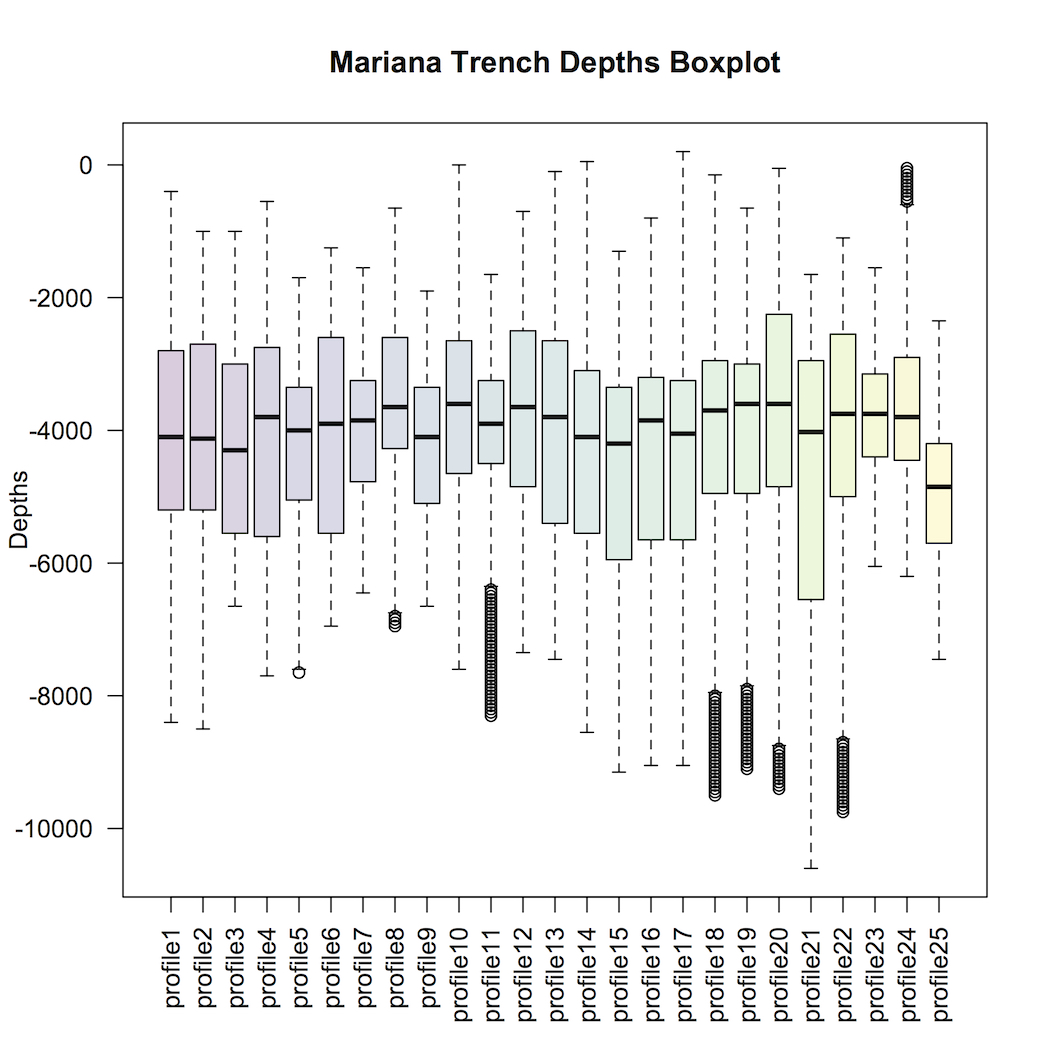
\includegraphics[width=0.6\textwidth]{Fig-4-3.jpg}
	\caption{Box plot histograms on data distribution, Mariana Trench bathymetric profiles 1:25. \\ Computed in R by code: \ref{R:02}}\label{fig:4-3}
\end{figure}

The R scripting is composed of separate written codes and an algorithm for data processing. The R codes presented below generate a call for various statistical formulae and algorithms used by the machine for the data processing.

	\subsection{Analysis of bathymetric data distribution}\label{ssec:RDDistr}
The data distribution for the bathymetric profiles has been computed using existing methods of the statistical analysis \cite{SwanSandilands1995} using R programming language. Depending on the structure and size of the availability data frame, the methodological approaches of the assessment of data distribution may change. However, the most essential statistical analysis of the ocean research would start by the question of data distribution. Computing and plotting Kernel distribution curves, box plots, regression lines (probability of bathymetric data across profiles), quantile statistics, empirical distribution density function and other methods can be distinguished as the most useful for initial data processing.

	\subsubsection{Box plots}\label{sssec:Rboxplot}
The created box plot of the depths distribution show summary statistics, that is range and quartiles of the observation points across the bathymetric profiles. A box plot (Fig. \ref{fig:4-3}) graphically displays the frequencies of a bathymetric observations data set of the 25 profiles of Mariana Trench. It plots frequency or count, on the depth y-axis (vertical) and the variable being measured on the x-axis, that is profiles (horizontal). The box plot was generated by the default R library (stat) graphically representing five the most important descriptive values for a bathymetric data set: \ref{R:02}. These values include the following bathymetric values: minimum value, the first quartile (0.25), the median, the third quartile (0.75), and the maximum value (that is, absolute depth). When graphing this five-number summary, only the horizontal axis displays values, while a vertical line is placed above each of the summary numbers showing depth values. A box is drawn around the middle three lines (first quartile, median, and third quartile) and two lines are drawn from the box’s edges to the two endpoints (minimum and maximum values of depths) using R code: \ref{R:02}

	\subsubsection{Histograms}\label{sssec:Rhist}
The histogram plots (Fig. \ref{fig:4-3-1}) show normal distribution of the depth observation data by the bathymetric cross-section profiles, as well as their outliers, skewness, median, mean, average, maximal, minimal and quartile distribution values. For each of 25 bathymetric profile various colors are taken for the following statistical data of depth values along the profile: ‘black’ curves stands for normal distribution, ‘blue’ curves – for density distribution. Vertical dashed lines: ‘purple’ – median values, ‘green’ – mean values. The histograms have been drawn using R library(ggplot2). On the first step a single histogram for each of bathymetric 25 profiles was created. The full R script to create one histogram is as follows (here: for the profile Nr. 1, further applied for every one from 25 profiles by changing the name of the file from ‘01’ to ‘02’, and so on to ‘25’). Using this script further 25 profiles have been created, consequently, p01, p02, ... p25. The combination of histograms of the 25 profiles on one layout was done using following R script: \ref{R:01} \cite{Lemenkova201991}. The histograms illustrate the frequency of the score occurrences in a continuous data set of the bathymetric depths that has been divided into classes showing variation in the samples of the depths, assumptions of the underlying statistical distribution of observation points values.

	\subsubsection{Violin plots}
The violin plots (Fig. \ref{R:25}) were created to show Kernel probability density distribution of the bathymetric observations, as multimodal distributions with multiple peaks. Kernel density distribution plot as shown on the Fig. 2 was created using library \{violinmplot\} of R in a combined plot, which includes calculated quantiles for 0.25 and 0.75 of the data pool. 
\begin{figure}[H]
	\centering
		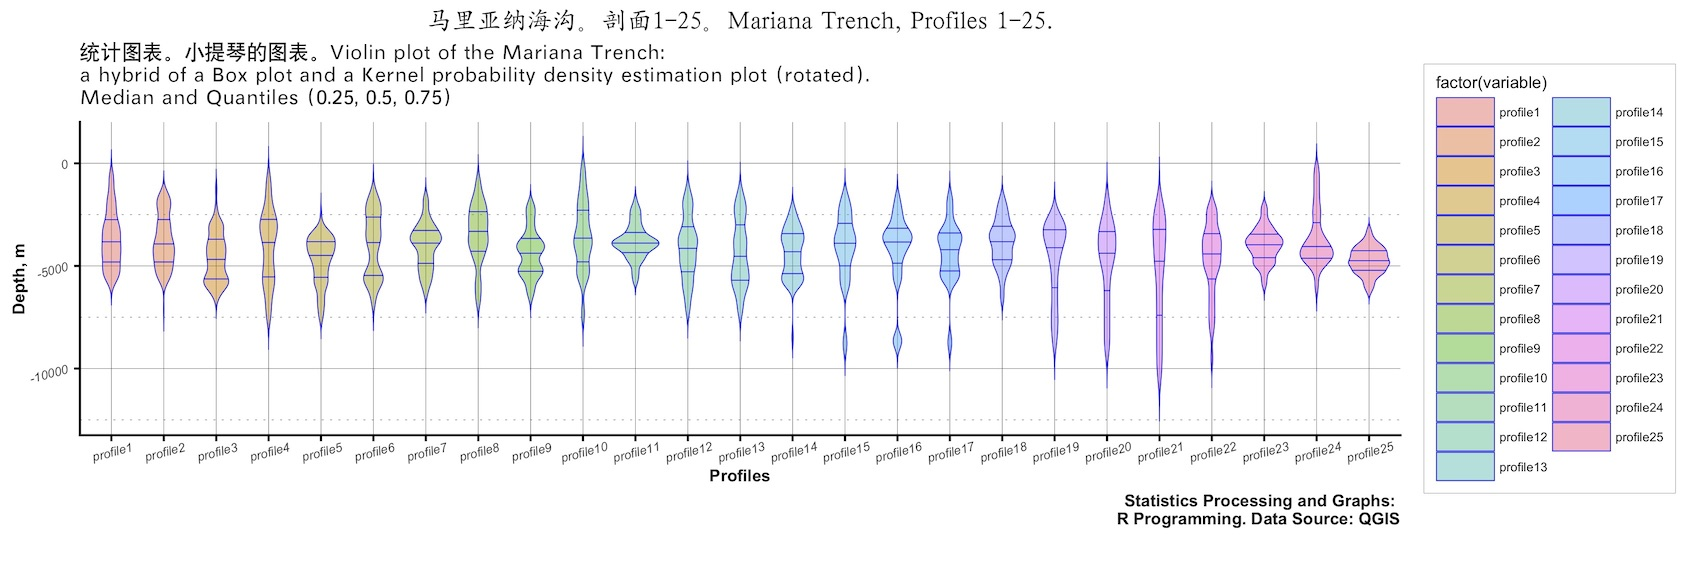
\includegraphics[width=13cm]{Fig-4-3-1b.jpg}\caption{Violin plots showing depth data distribution for observation points of the 25 bathymetric profiles of the Mariana Trench. Computed in R by code: \ref{R:25}}\label{fig:4-3-1b}
\end{figure}

	\subsubsection{Notched box plots}
Another way of representing box plots is so called 'notched box plots'. The notched box plots computed and visualized in R by \ref{R:03} aimed to show distribution of the depths with majority of the data from -3000 to -5000 m and outliers (the deepest points) show that from profile 1 to 16 the general depth increase with deepest values at profiles 10 and 11. The notched box plot on Fig. 6 shows the shallowest parts of the trench are located in the profiles 24 and 25 where Mariana Trench crosses the Yap Trench, the oceanic trench near Yap Island in the western Pacific Ocean, \cite{Lemenkova201991}.

	\subsection{\ac{KDE}}\label{ssec:RKDE}
The \ac{KDE} is a non-parametric way to estimate the probability density function of a random variable of the observation depth. The \ac{KDE} has been performed by smoothing data points across the sample points in the profiles 1:25 of the Mariana Trench. The \ac{KDE} can be endowed with properties such as smoothness or continuity of the bathymetric data by using a suitable kernel. Technically, besides \{violinplot) library, a kernel density estimation function can be implemented in R through the density, the \{bkde) function in the \{KernSmooth\} library, as well as through the \{kde\} function in the \{ks\} library: Fig. \ref{fig:4-3-1k}. To use the \{kde.R\} function, it is not required to install any packages or libraries, while \{violinplot\} package was installed and activated prior to the current work. The \ac{KDE} shows the majority of the depths of the trench between 3000 and 6000 m. The graph has been made as a combined plot (Figure \ref{fig:4-3-1k}) enabling to compare the overlapping and maximal aptitude of the density curves both for the profiles and depth data distribution by four tectonic plates. 

\begin{figure}[H]
	\centering
		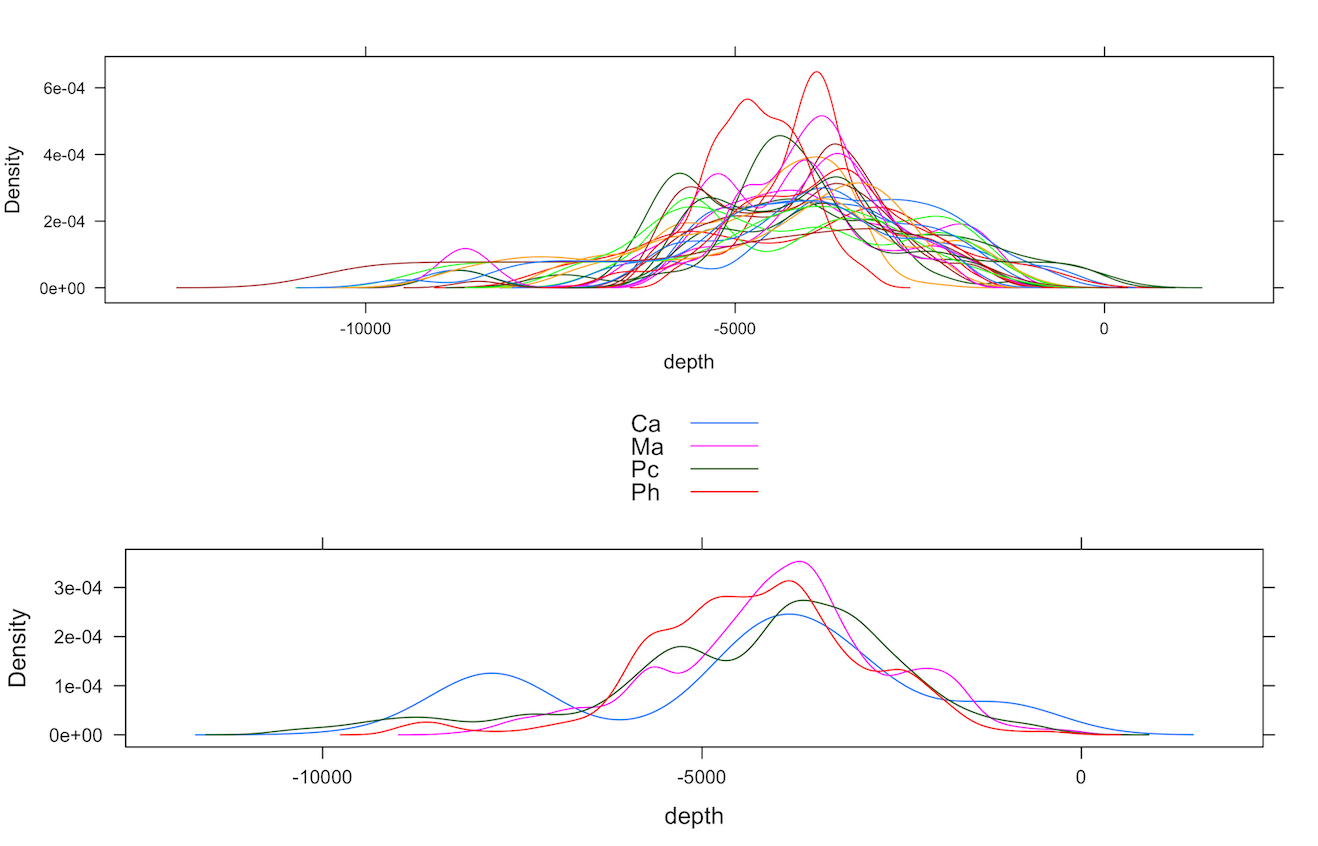
\includegraphics[width=14cm]{Fig-4-3-1k.jpg}
	\caption{Kernel density estimation for 25 bathymetric profiles. Computed in R by code: \ref{R:19}}\label{fig:4-3-1k}
\end{figure}

	\subsection{Regression analysis}\label{ssec:RA}
To estimate the relationships between variables a regression analysis has been done using existing methods \cite{Journel2000}. The principle of the regression analysis is based on the analysis of the probability of the
data values according to their actual distribution. A regression analysis represents outlying depths observations by each bathymetric profile, as shown on the example of three profiles in Figure 4. This methodology utilizes the relation between two or more quantitative depth variables so that one variable can be predicted from another. Thus, one can estimate the probability that the depth values will be located in this or that interval of values profile by profile according to the machine-based algorithm of the probability of their distribution. Regression analysis and facetted plot wrapping for 25 bathymetric profiles were executed by R library (ggplot2). Using non-parametric regression analysis the conditional expectation of the dependent variable (that is depth values) given the independent variables was estimated. The confidence interval for each of 25 profiles has been done by four methods, visualized by the facetted plot wrapping for the series data comparison.
The regression analysis reveals how the typical value of the criterion variable changes when any one of the independent variables change, while the other independent variables are fixed. The formula describing regression equation describing the relationship between two variables used in this research is as follows:

	\begin{equation}
		Y=a + bX + e(1)
	\end{equation}\label{eq:5}\myequations{Linear regression analysis formula}
	
The literature refers \cite{Journel2000} to three major applications of the regression analysis including general loess method ('glm), loess method ('lm') and loess method ('loess'), all of which were tested in this research. The quantiles were drawn by calling (geom-quantile) function of R \ref{fig:4-3-2b}. The generalized linear models (glm method) was used to give a symbolic description of the linear predictor of depth variability within each bathymetric profile, and a description of the error distribution in a range of the depth observation points. The quantiles graphically depict groups of the depth values through their distribution mode, according to the methods of the descriptive statistics. The spacings between the different parts of the box indicate the degree of the dispersion, i.e. spread, and skewness in the bathymetric data, and show outliers. The data outside the upper and lower quartiles are the outliers that are plotted as individual points. The outliers are the non-usual values of the depths indicating specific features of the geomorphology with extra deep values. The histograms show probability of the density distribution of the bathymetric observation by the profiles, i.e. how likely is that the data will belong to this or that part of the group values within certain depth range.

	\subsection{Comparative geospatial analysis by tectonic plates}\label{ssec:CA}
Mariana Trench crosses four tectonic plates: Mariana, Philippine, Pacific and Caroline. Therefore, a comparative analysis of multidimensional data was performed to analyze inter-relationships between the geographic location of the specific parts of the trench and factors that may impact changes in the geomorphic systems. Using existing methodology \cite{Bretzetal2011}, various dependences between the impact factors were tested in the current research by various approaches of the comparative analysis: Fig. 7 in \cite{Lemenkova201991}. First, the distribution of various environmental factors affecting the morphology of the trench were analyzed: slope angle, sedimental thickness, depth and closeness of the igneous volcanic zones to the selected bathymetric profiles.\\
Second, the changes in the trench deepest angle, calculated as tg(A/H), where A is the width, and H is the maximal depth of the profile, were calculated for each of the 25 bathymetric profiles and compared, respectively. Third, the depth distribution by four tectonics plates was visualized using multiple scatter function of R. A pairwise correlation of the environmental factors was performed by the scripting approach of R, which is convenient not only for looping over parts of the geomorphic model of the Mariana Trench, but also for pairwise iterating over bathymetric and geomorphic variables for the comparative analysis. Called functions 'geom-smooth', 'geom-point' and 'geom-quantile' were used to draw smoothed conditional means and to perform regression analysis. The multiple panel strip plots were generated in a combined plot using {LatticeExtra2} package of R by strip plot function. \\
The distribution of the slope angle, sediment thickness, depth and closeness of the igneous volcanic zones towards Mariana Trench, by four tectonic plates is shown on Fig. 7 in \cite{Lemenkova201991}. It shows distribution of slope angle, sedimental thickness, depth and igneous volcanic zones, by four tectonic platesThe R code used: \ref{R:17}. The multiple panel by groups analyzing four tectonic plates, trench slope angle in the deepest point, depth scope (min-max) by profiles using overlapping points, are computed and visualized in R code: \ref{R:18}. The variation of the slope angle in the deepest point and depths by 25 bathymetric profiles of the Mariana Trench according to four tectonic plates that is crosses is illustrated on Fig. 8 and Fig. 9 in \cite{Lemenkova201991}. The graphs show variation of the slope angle in the deepest point and depths by bathymetric profiles of the Mariana Trench for four tectonic plates: Mariana, Caroline, Pacific and Philippine, respectively.

	\subsection{Ridgeline, categorywise and circular plots}\label{ssec:CW}
The ridge plots (R: \ref{R:35}) combine information about statistical data on 25 bathymetric profiles: arithmetic density distribution, mean and standard deviation along the profiles in a facetted way, (Fig. 10 in \cite{Lemenkova201991}. They have lines extending horizontally from the boxes indicating variability of the depths distribution across all the profiles. The code generated using (ggridges) and (ggplot2) libraries by R code \ref{R:35}. To create categorywise plot, first, the table was read into R: Second, the tables columns were merged calling \{merge\} function from library(data.table) by environmental variables: depth, tectonics, slope angles. Then the new data frame (DFDT) was created. Third, the plot function was called by the following code using created data frame in the previous step: \ref{R:13} and finally the graph visualized (Fig. 12 in \cite{Lemenkova201991}, left. \\
A \{tidyverse\}, another R package, was used to visualize a circular plot showing the comparative analysis of the bathymetric ranged by the sediment thickness. The algorithms and syntax of R coding was applied from the R manuals and available materials \cite{RCoreTeam2014}; \cite{KleiberZeileis2008}. The circular bar plot showing distribution of depth on the tectonic plates (Fig. 12 in \cite{Lemenkova201991} right, shows the percentage distribution of the sediment thickness according to the slope angle steepnesss by 25 bathymetric profiles. It has been drawn using R library \{tidyverse\}. To create circular barplot divided by groups the following full R code was used by library(tidyverse): R: \ref{R:16}.

	\subsection{Ternary diagrams, radar and pairwise double-Y axis charts}\label{ssec:Ter}
Ternary diagrams and Radar chart show the triple correlation of several factors across tectonic plates: slope morphology classes, tectonics, igneous volcanic areas, aspect degree, slope angle, sedimental thickness. The programming R code for the ternary diagrams is R: \ref{R:29} and for the radar chart by (fmsb) library: \ref{R:21}. The pairwise double-Y axis was enables to analyze the effect of the bi-factor correlation between the slope angle and other variables. The following script runs the model in each case, calculates the X-Y dependences and places both graph on one plot, which his very convenient for comparative studies. The following is a code for the double-Y axis with correlations "Slope angle", "Sedimental thickness" created by library(latticeExtra) in R in consecutive steps: \ref{R:15}. At the end of each run, the final results are copied to the p1, p2 and p3 plot, and afterwards combined three graphs on one plot,  \cite{Lemenkova201991}.

	\subsection{Dumbbell charts for data pairwise comparison by tectonic plates}\label{ssec:Dum}
Because Mariana Trench crosses four tectonic plates (Mariana, Caroline, Philippine and Pacific) the comparative testing of the values distribution by adjacent tectonic plates has been completed through the Dumbbell chart plotting. Dumbbell chart is a visualization aimed to give an insight of how the margin tectonic plates constitute to the Mariana Trench pairwise. It is one of the new statistical methods that initially was widely used in biosciences, yet can be applied to spatial analyses when it is necessary to take pairwise comparison of the data distribution from any thematic layer. Plotting has been carried out by calling R libraries \{ggplot2\} and \{ggalt\} by code: \ref{R:12}. Dumbbell chart demonstrates pairwise distribution of the bathymetric points constituting the continental plates, to show the composition of the sedimentary coverage by four tectonic plates \cite{Lemenkova201904}. 

	\subsection{Ranking dot plots by data grouping}\label{ssec:Dot}
	Pairwise correlation was visualized by the ranking dot plots, which is effective tool to perform data grouping by variables: tectonic plates. Plotting distribution of the observation points by igneous volcanic areas aimed at visualizing areas affected by the magmatism. Large igneous volcanic areas contribute towards localization of possible earthquake zones. Thus, as can be drawn from the plot (Figure \ref{fig:4-3-R}), the volcanic areas increase along Mariana Trench south-westwards. Alike to the volcanic areas plotting, the variation of the steepness slope was performed using ranking dot plot: the bathymetric profiles with the most steep angles across the trench are located in the north-eastern part with a slight decrease towards the south-west. To calculate tg \degree angle of the profiles, a standardized formula was used, that is a relation of the maximal depth by profiles divided by the width of the corresponding bathymetric profile. 
	
\begin{figure}[H]
	\centering
		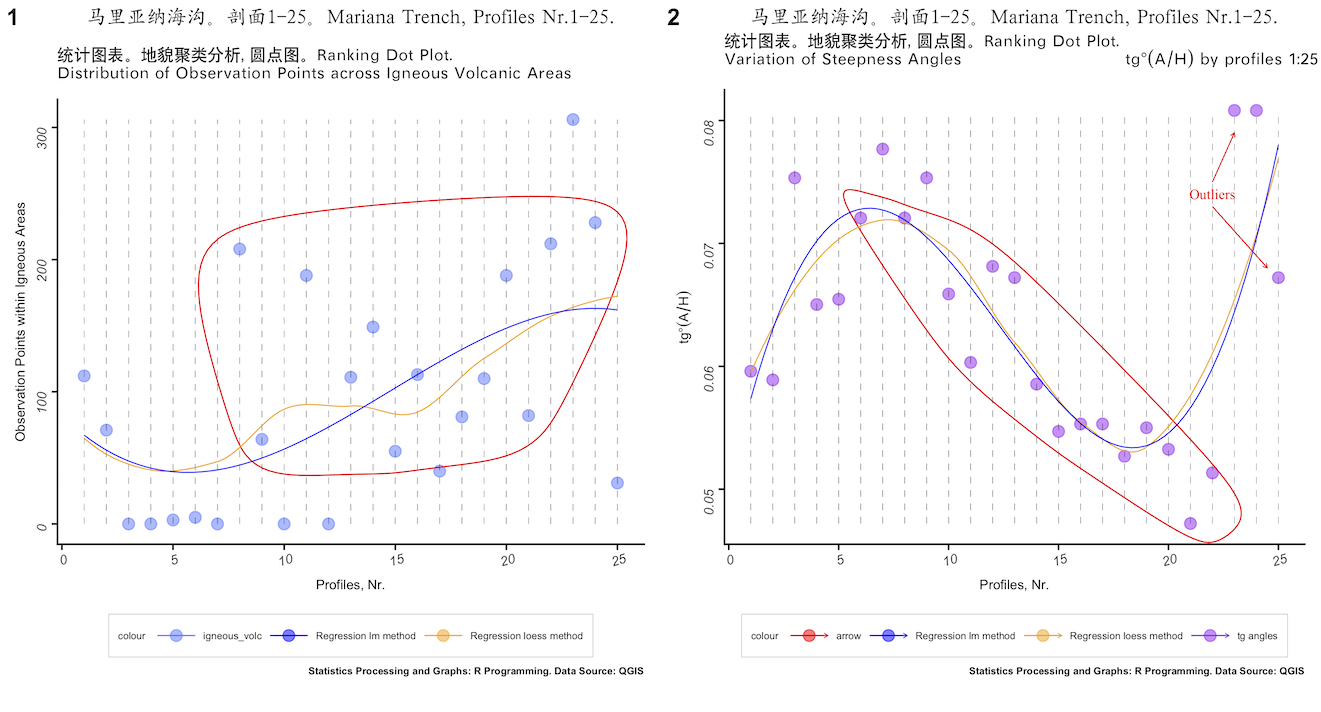
\includegraphics[width=14cm]{Fig-4-3-R.jpg}
	\caption{Ranking dot plots by data grouping. Computed and visualized in R: \ref{R:14}}\label{fig:4-3-R}
\end{figure}

	The crucial points (Figure \ref{fig:4-3-R}) were selected using library \{ggalt\} by calling following R code: \ref{R:14}. The distribution of angle steepness values across the trench have been shaped by the components of the igneous volcanic areas near the profiles, as understood from the Figure \ref{fig:4-3-R}: profiles \# 20, 22, 24, 8 and 11 with notable amount of igneous volcanic observation points (over 180) correlate with steepness angle.
	
\subsection{Ranking data for variation of the geomorphic steepness: }
Geomorphic variation distinguishes a certain segment of the profile across the trench from neighboring areas. A variation in geomorphology is changes in shape that varies from one segment to another depending on the tectonic properties and geodetic location. The geological analysis alone is not sufficient for modelling the geomorphic variations within the trench area, since other factors, such as bathymetric depth and geolocation should be concerned. The correlation between the geomorphic shape with geologic settings and geographic location revealed that the submarine geomorphology of the Mariana Trench is generally influenced by the geospatial settings of the underlying tectonic plates that affect its shape and cause variation of the steepness across the trench segments. The variation of the shape form is also strongly affected by the geodetic location of the trench crescent.\\
The variations in the presented bathymetric profiles shows (Figure \ref{fig:4-3-17}) trench varies in shape across its crescent: five divided regions varying in steepness degree, ranging from the strong slope, very strong slope, extreme slope and very steep slope. The unsorted spatial series of the profiles (Figure \ref{fig:GP-6}, left) only shows the consequent distribution of the slopes, so we cannot judge their variations, but only general range. Upon sorting and ranking profiles (Figure \ref{fig:4-3-17}, right), the segments with similar geomorphic slope steepness are ranked and grouped. Ranking data was based on the geomorphic steepness using R libraries and existing mathematical algorithms \cite{RCoreTeam2014}. The methodology for plotting Figure \ref{fig:4-3-17} consists in the application of the R code \ref{R:22}.

\subsection{Compositional charts of the determinants variations}\label{ssec:Waf}
	The constitution of the system composition has been visualized by the categorical plotting. One of the methods enabling categorical plotting is presented by compositional charts, sometimes referred to as “waffle charts”. 
	
\begin{figure}[H]
	\centering
		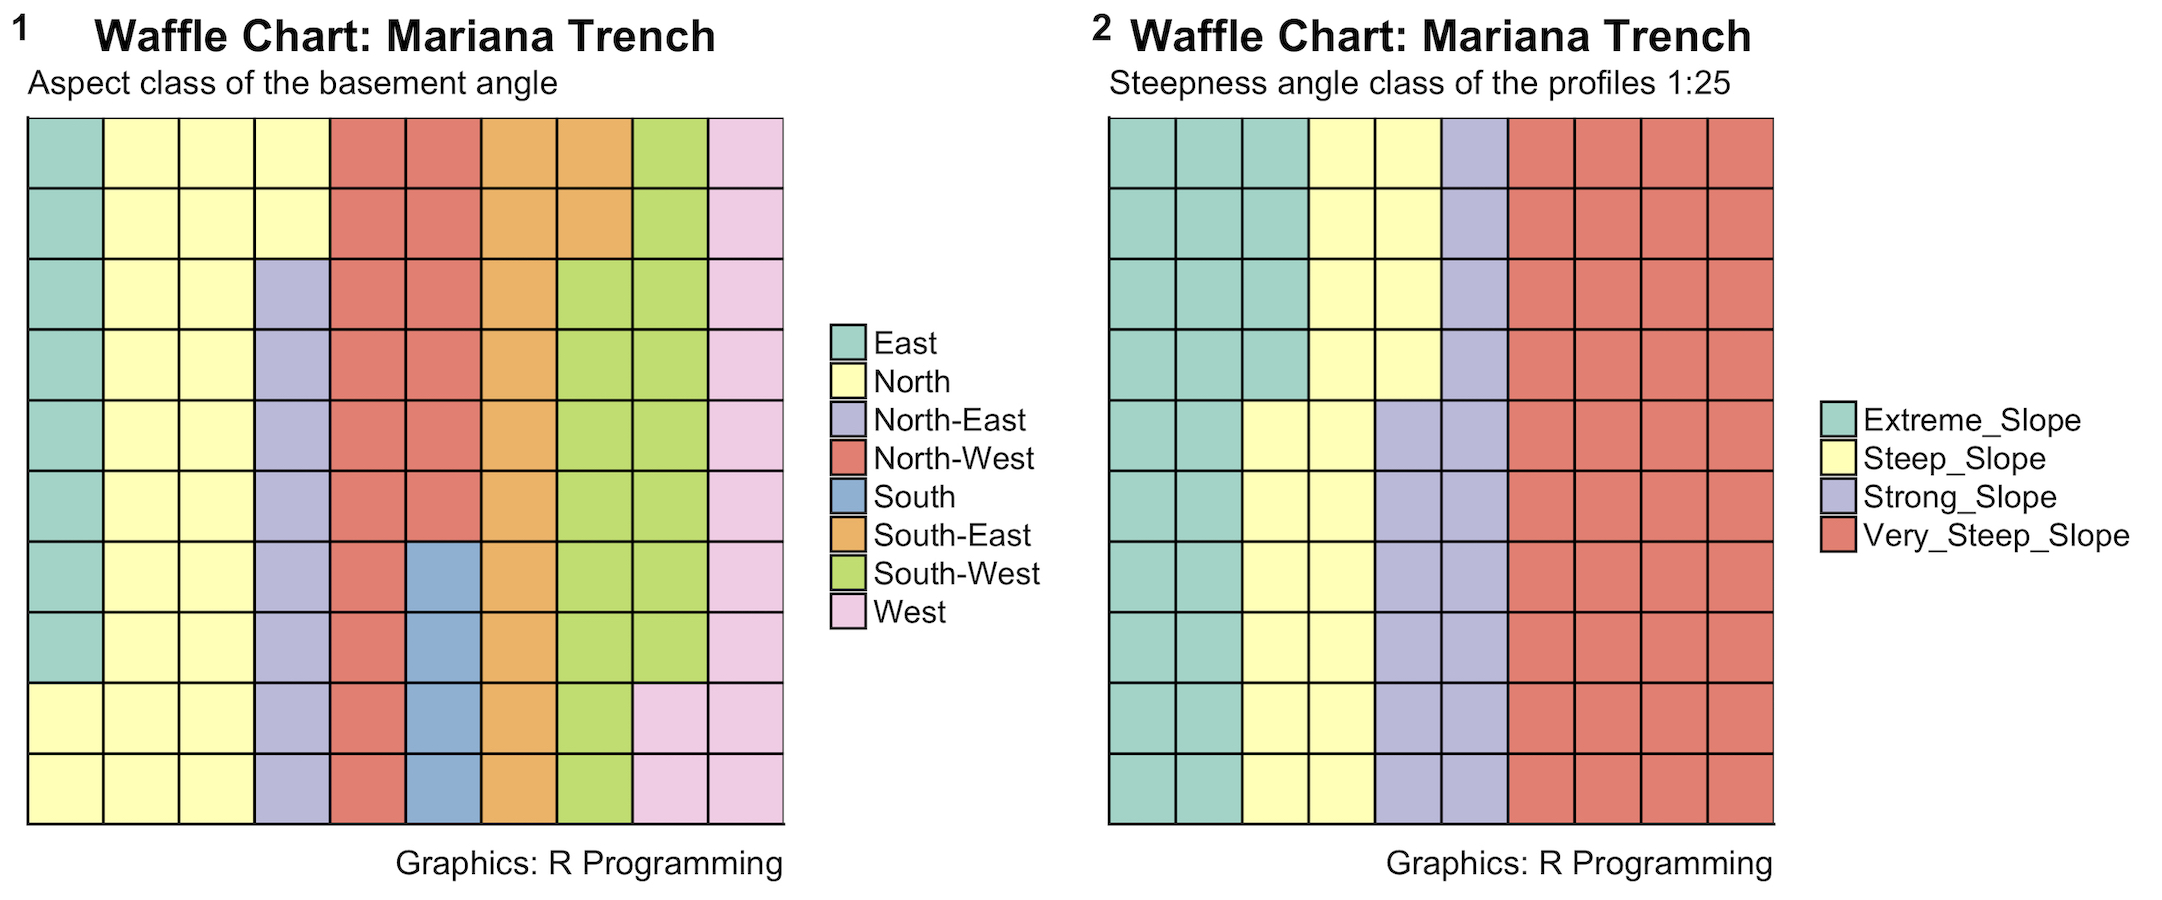
\includegraphics[width=15cm]{Fig-4-3-W.jpg}
	\caption{Compositional chart of geometric properties of the Mariana Trench. Computed and visualized in R}\label{fig:4-3-W}
\end{figure}

	 The core idea of this method is to demonstrate the division of the whole system by parts in percentage. Several R libraries can be used to perform technically compositional plotting, of which the \{ggplot2\} has been selected as the most effective (\ref{R:37}) comparing to the \{waffle\} library (\ref{R:38}): it enables to control the appearance of the plot by adjusting details (colors, font size and types, plotting two graphs together, etc). The compositional chart is aimed to compare the distribution of the data across the study area, as well as the composition of the aspect class and slope angle for the Mariana Trench. As can be drawn from the chart (Figure \ref{fig:4-3-W}), the category “very steep slope” is the dominant among all other geomorphological types of the slope degree of the Mariana Trench. Likewise, north and south-west aspect of the slope direction are best describing the geometry of the northern and southern part of the trench, respectively.
	
	\subsection{Mosaic, silhouette and association plots}\label{ssec:Mos}
	Mosaic chart aims at categorial comparison of the geomorphological features of the trench by four tectonic plates. Visualizing mosaic plot is a statistical method that involves a subdivision of a rectangular tiles into the areas that represent the conditional relative frequency for a cell in the contingency table. The algorithms and approaches used in mosaic plotting vary slightly. Upon examination of possible packages, the R library \{vcd\} was selected for this research (R code: \ref{R:31}). Using {vcd} library, each tile is colored to show the deviation from the expected frequency, that is residuals, from a Pearson X2 or likelihood ratio G2 test. The algorithm set includes execution of the following code:\\ The convenience of the mosaic plot for the geomorphological analysis of the ocean trenches consists in its visual representation of the association between the environmental variables. Thus, it gives an overview of the data structure and enables to recognize relationships between the different environmental variables.  \\
Conversely, the boxes across categories constituting Pacific and Mariana plates have similar areas. The area of the tiles, the bin size, includes the identification of the sampling data, giving the proportional value to the number of observations within that category.\\
The interpretation and validation of consistency within clusters of geomorphologic and geological variables have beet tested using silhouette method. This technique provides a succinct graphical representation of the suitability and fitness of each from 518 observation points across 25 bathymetric profiles within the clusters. The silhouette value measured similarity of the points derived from the thematic layers (sediment thickness, slope steepness of the trench) to the cluster by cohesion and comparison them with other clusters, and separating them from the distinct points. Lower sediment thickness area would lie within one class while a class of areas with high level of sedimental level fits to another. The silhouette was calculated with Euclidean distance metric by calling library \{cluster\} using following R code: \ref{R:30}. The given script plots the silhouettes, returns the values in the n-by-1 vectors.\\
A deviations from the independence of rows and columns containing bathymetric data and environmental variables is presented in a two-dimensional contingency table of the Cohen-Friendly association plots. Extended association plot in R reveals relationships between the variables by the assoc() function in the \{vcd\} package. In this case, it is tectonic plates and geomorphological values (bathymetric depths, slope steepness). Pearson's residuals on the association plot report test for the statistical goodness of fit: it enables to assess the model fit at each of samples for each profile for the generalized linear models within the context of the chi- square, as shown further in \cite{Lemenkova201904}. It has been computed as a raw residual divided by the square root of the variance function. Technically, association plot method includes execution of the following R code: \ref{R:31}.
	
\subsection{Clustering (k-means method), correlation ellipses and data partition}\label{ssec:Ckme}
	The next working step included finding correlations among the geomorphic factors that impact the morphological formation of the profiles. To this end, cluster analysis and correlation ellipses were created.
	\paragraph{Clustering (k-means method) by R library(facto-extra)}
The k-means clustering, a machine learning technique for classification performs data partition into set up number of clusters, has been done using R library (factoextra). The goal of the k-means clustering was to perform partition of the dataset of the observations across Mariana Trench into clusters, in which each depth observation belongs to the cluster with the nearest mean, serving as a prototype of the cluster. The performed clustering is sensitive to the initial random selection of the cluster centers. Therefore, several clusters has been tested: starting from 2 to 7. This function provides a solution using a hybrid approach by combining the hierarchical clustering and the k-means methods. The workflow procedure include following steps: Tab. \ref{tab:T6}.

\begin{table}
\caption{Statistical algorithm of clustering, R code: \ref{R:09}}\label{tab:T6}
\begin{tabular}{@{\makebox[1.5em][r]{\rownumber\space}} | p{12cm} }
\multicolumn{1}{@{\makebox[1.5em][r]{No}} | l}{Step} \\ 
		\arrayrulecolor[RGB]{165,154,202}\hline\hline				
        Computed hierarchical clustering and cutting the tree in the k-clusters \\              
       		\arrayrulecolor[RGB]{0,123,187}\hline					
        Computed pairwise standard scatter plot of k-means cluster correlation \\           
        		\arrayrulecolor[RGB]{126,190,165}\hline
	Computed pairwise standard scatter plot of k-means cluster correlation \\           
        		\arrayrulecolor[RGB]{126,190,165}\hline
	Computed centers (2 to 7 were tested, in total 6 centers) of each cluster\\  
        		\arrayrulecolor[RGB]{126,190,165}\hline
	Created groups of the correlation matrix tested by distributions on the plates \\           
        		\arrayrulecolor[RGB]{126,190,165}\hline\hline
\end{tabular}
\end{table}
The k-means of the clustering of the Mariana Trench profiles was computed and visualized in R by code \ref{R:09}, Fig. 14, the k-means clustering with different k-values is shown on Fig. 15, \cite{Lemenkova201991}. The K-means cluster analysis has been performed using set of cluster centers as the initial cluster centers. The algorithm worked iteratively to assign each profile to one of the groups (2 to 7) based on the morphometric features of the Mariana Trench across these profiles that were clustered based on their geomorphic feature similarity. The results of the k-means clustering are shown on the Fig. 15, further details are given in \cite{Lemenkova201991}. The pairwise standard scatter plot of k-means cluster correlation distributed by four tectonic plates is shown on Figure \ref{fig:4-3-14}. 

\begin{figure}[H]
	\centering
		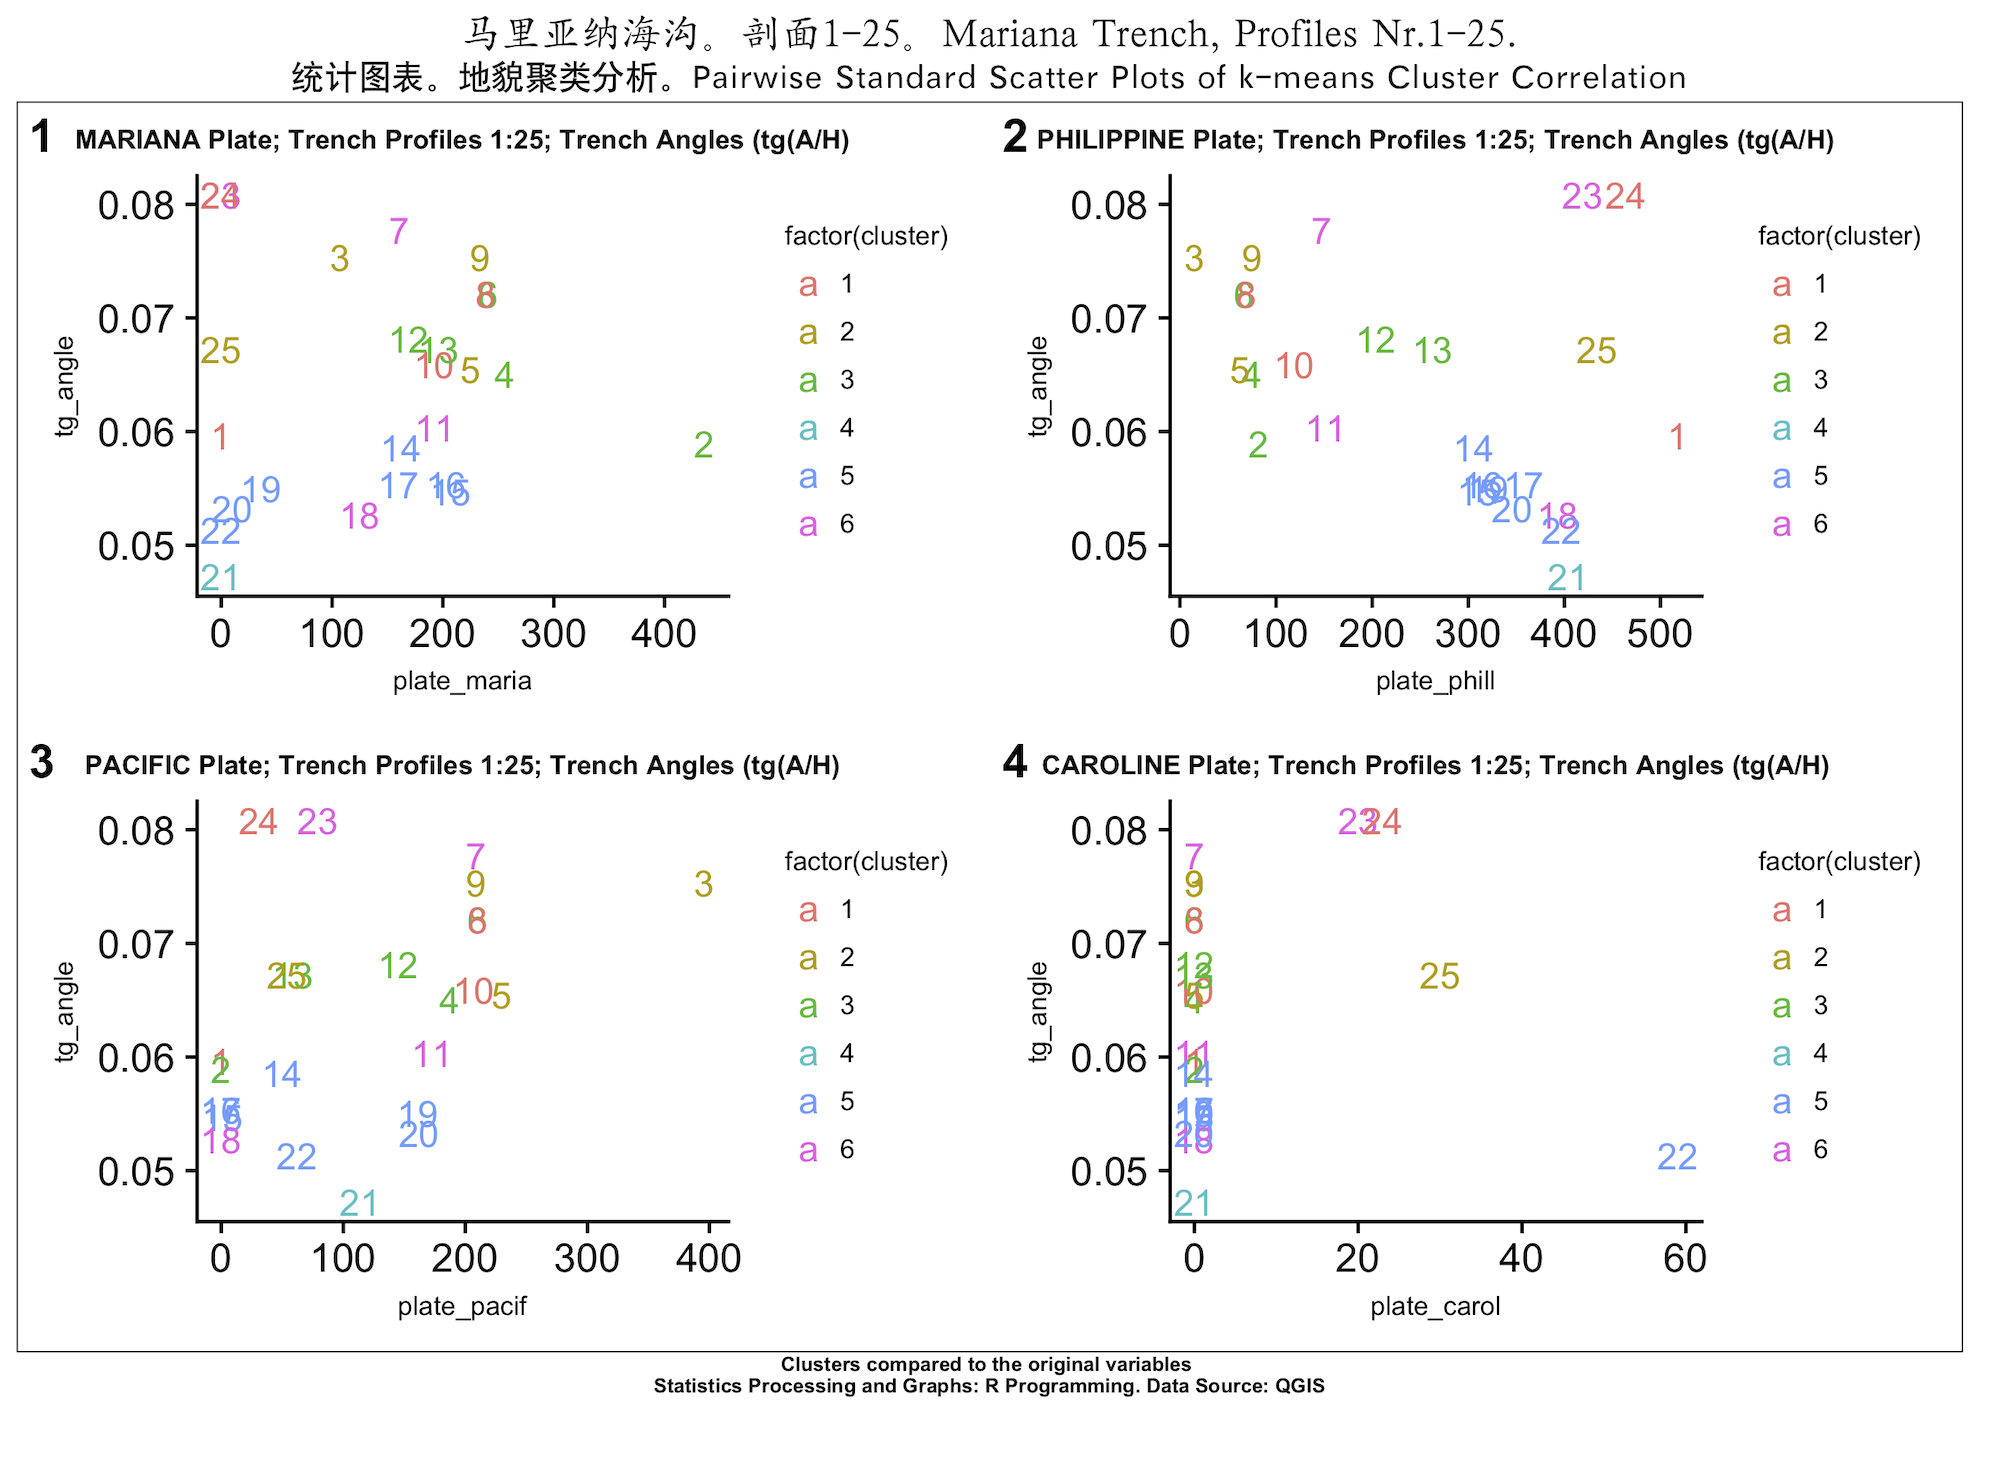
\includegraphics[width=12cm]{Fig-4-3-14.jpg}
	\caption{Classification of the k-means clustering of the Mariana Trench by tectonic plates. Computed and visualized in R: \ref{R:09}}\label{fig:4-3-14}
\end{figure}

The k-means cluster analysis has been done using following R code: \ref{R:09}.
The advantages of the k-means clustering applied for Mariana Trench consists in the algorithm nature: rather than defining groups before looking at the data, clustering enabled to find and analyze the groups in the profiles that have formed organically. As the structure of the tectonics and trench geomorphic properties are rather complex, clustering facilitated data partition and grouping.

\subsection{Correlogram Ellipses and Numerical Correlogram}\label{ssec:CorrE}
The correlogram ellipses were generated to visualize correlation between the factors affecting the morphology of the trench \cite{Lemenkova201991}. The methodological approach includes calling \{ellipse\} library and executing following script: \ref{R:32}.

\subsection{Hexagonal plots and data partition}\label{ssec:Py04}
Plotting hexagonal plot was performed using R language using specially designed library \{hexbin\}. This plot aims to show how the bathymetric data are distributed by the profiles in terms of frequency: i.e. how often the values are being repeated by profiles. 

\begin{figure}[H]
	\centering
		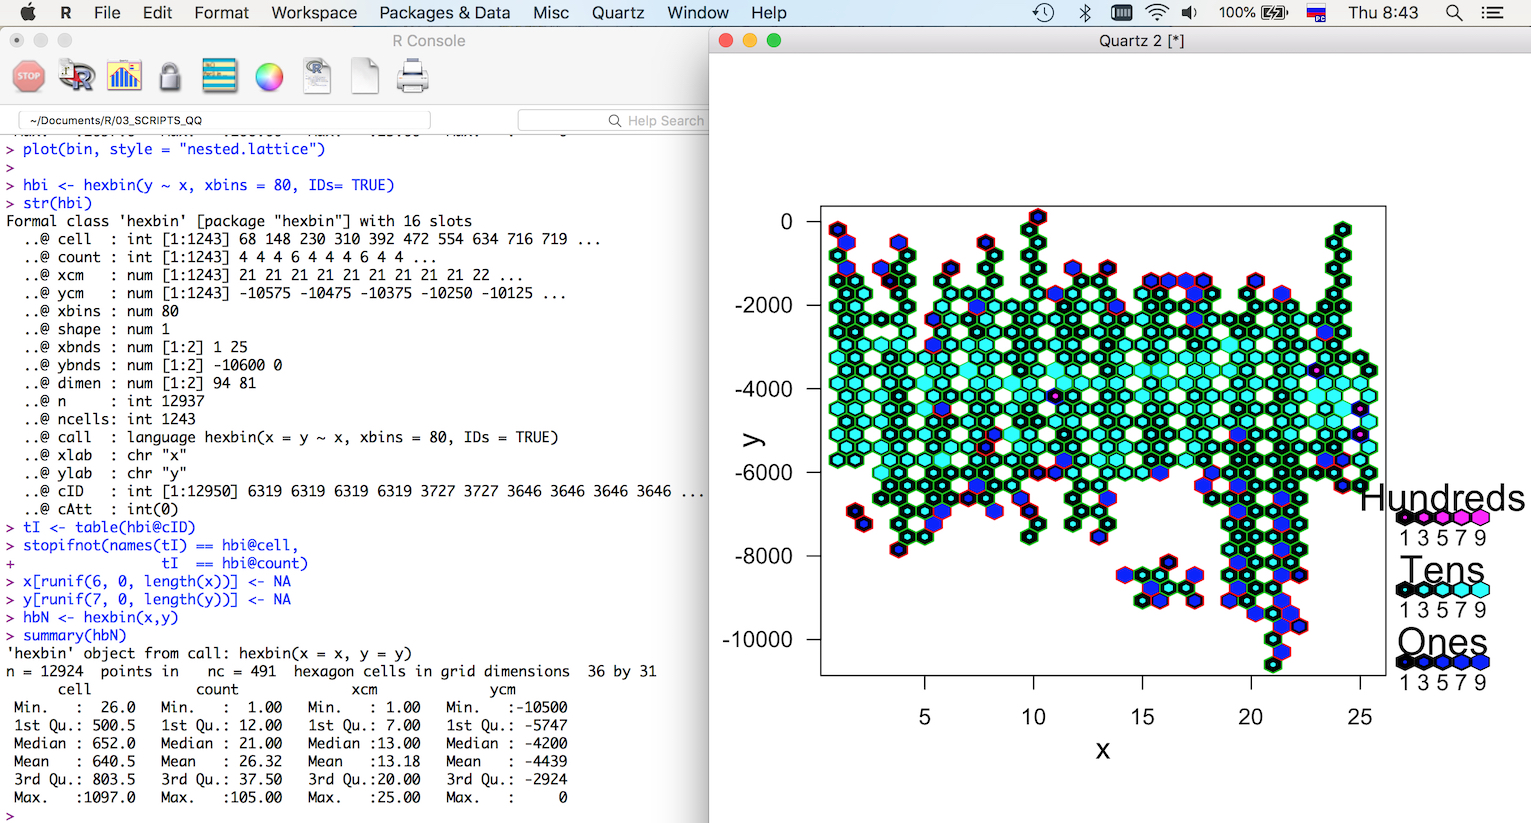
\includegraphics[width=13cm,clip]{Fig-COMU-5.jpg}
	\caption{Hexagonal data distribution: plotting by R language, \{hexbin\} library.}\label{fig:COMU-5}
\end{figure}

Hexbin plots serve as a useful alternative to scatter plots, as the data are are dense. Therefore, plotting each point individually in this case is not effective: the data would be indistinguishable on the graph. Hence, the \{hexbin\} library was used to plot the range of the depths values within Mariana Trench using the R code: \ref{R:27}. Studies revealed that multiple factors affect Mariana Trench geomorphology. The statistical analysis performed by Python and R languages revealed that the major depth observation points of the Mariana Trench are located in between the -3000 and -5000 meters (Figure \ref{fig:COMU-4} and Figure \ref{fig:COMU-5}), as also discussed by \cite{Gross2016}. The significant point is that sediment thickness changes notably both within the trench by profiles (1:25) and between four tectonic plates that Mariana Trench crosses: Philippine, Pacific, Mariana and Caroline. \\
Data grouping and partition has been performed by dividing angles across the trench on to classes (Fig. 19 left \cite{Lemenkova201991}). The level plot (Fig. 19 right \cite{Lemenkova201991}) shows the classes on the sediment thickness across the Mariana Trench has been built by R code: \ref{R:33}.
	
\subsection{Calculation of the normalized steepness angle of the Mariana Trench}\label{ssec:Steep}
The normalized steepness was computed as a steepness of dominance hierarchies of slope angle (Fig.\ref{fig:4-4}). Steepness is defined as the absolute slope of the straight line fitted to the normalized scores. The normalized scores were obtained on the basis of dominance indices corrected for chance or by means of proportions of wins. Given an observed data set, it computes hierarchy's steepness and estimates statistical significance by means of a randomization test.
\begin{figure}[H]
	\centering
		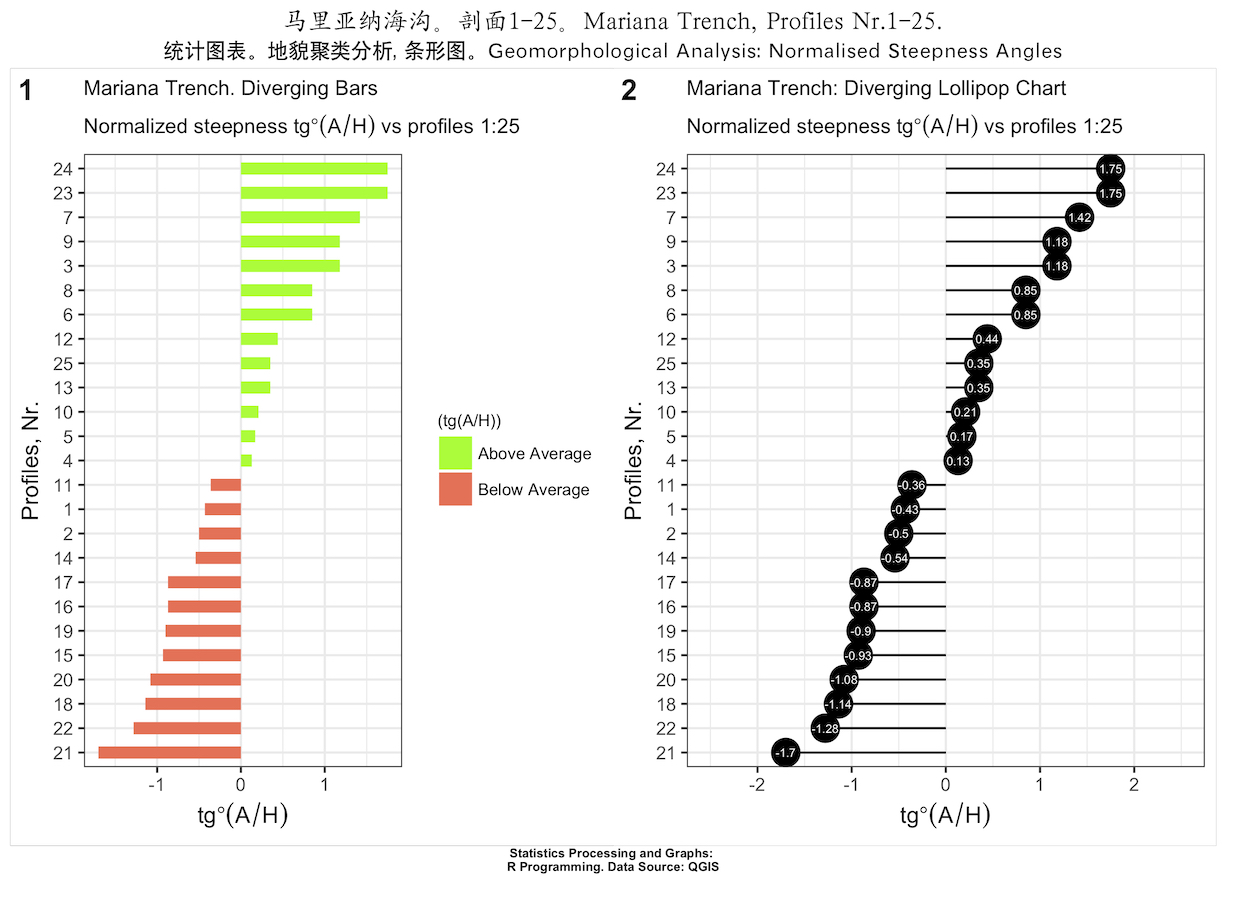
\includegraphics[width=13cm]{Fig-4-4.jpg}
	\caption{Normalized steepness slope angle, bathymetric profiles 1:25 of the Mariana Trench.\\ Computed in R by code}\label{fig:4-4}
\end{figure}

	\subsection{Correlation analysis of impact factors}\label{ssec:Corr3}
Correlation coefficient is a numerical measure of direction and strength of linear correlation between various environmental variables, i.e. how strong a relationship is between geomorphological, bathymetric and geological variables is across four different tectonic plates. Three methods of computing correlation analysis were tested: Pearson correlation, Spearman correlation, Kendall correlation \cite{Lemenkova201868}. Additionally, numerical correlogram, correlation and cross-correlations matrices were generated to analyze environmental impact factors for the Mariana Trench. The correlogram matrices are computed and visualized by R scripting libraries. 

	\subsubsection{Computing Pearson correlation}\label{sssec:Pear}
Developed by Karl Pearson from a related idea of Francis Galton in the 1880s, a Pearson product moment correlation coefficient, also know as the bivariate correlation, is a measure of the linear correlation between two variables:\\

	\begin{equation}
		r=\frac{\displaystyle \sum(x-mx)(y-my)}{\sqrt{\displaystyle \sum(x-mx)2\displaystyle \sum(y-n)}}
	\end{equation}\label{eq:6}\myequations{Pearson correlation coefficient}
	
In this case the environmental variables have been tested by the Pearson correlation: sedimental thickness, slope angle, slope class, aspect degree, hill shade in values, location of igneous volcanic zones across the abyssal valley, tectonics by four plates (Mariana, Caroline, Philippine and Pacific), a bunch of bathymetric values, that is maximal and minimal depth values, median means value for each profile, $\tan$ angle \degree. Pearson correlation has a value between +1 and −1, where 1 is total positive linear correlation, 0 is no linear correlation, and −1 is total negative linear correlation. It has been presented on Fig.\ref{fig:4-56} It was computed and visualized by calling following R programming script: \ref{R:41}.

	\subsubsection{Computing Spearman rank correlation coefficient $\rho$}\label{sssec:Spear}
In this case the environmental variables have been tested by the Spearman rank correlation coefficient $\rho$: sedimental thickness, slope angle, slope class, aspect degree, hill shade in values, location of igneous volcanic zones across the abyssal valley, tectonics by four plates (Mariana, Caroline, Philippine and Pacific), a bunch of bathymetric values, that is maximal and minimal depth values, median means value for each profile, $\tan$ angle \degree. Named after Charles Spearman, a Spearman non-parametric $\rho$ coefficient is handling ties between the variables less properly comparing to previously computed Pearson coefficient (Fig.\ref{fig:4-56}). The Spearman's $\rho$ has been computed on sets of paired rankings between the environmental factors. 

\begin{figure}[H]
	\centering
		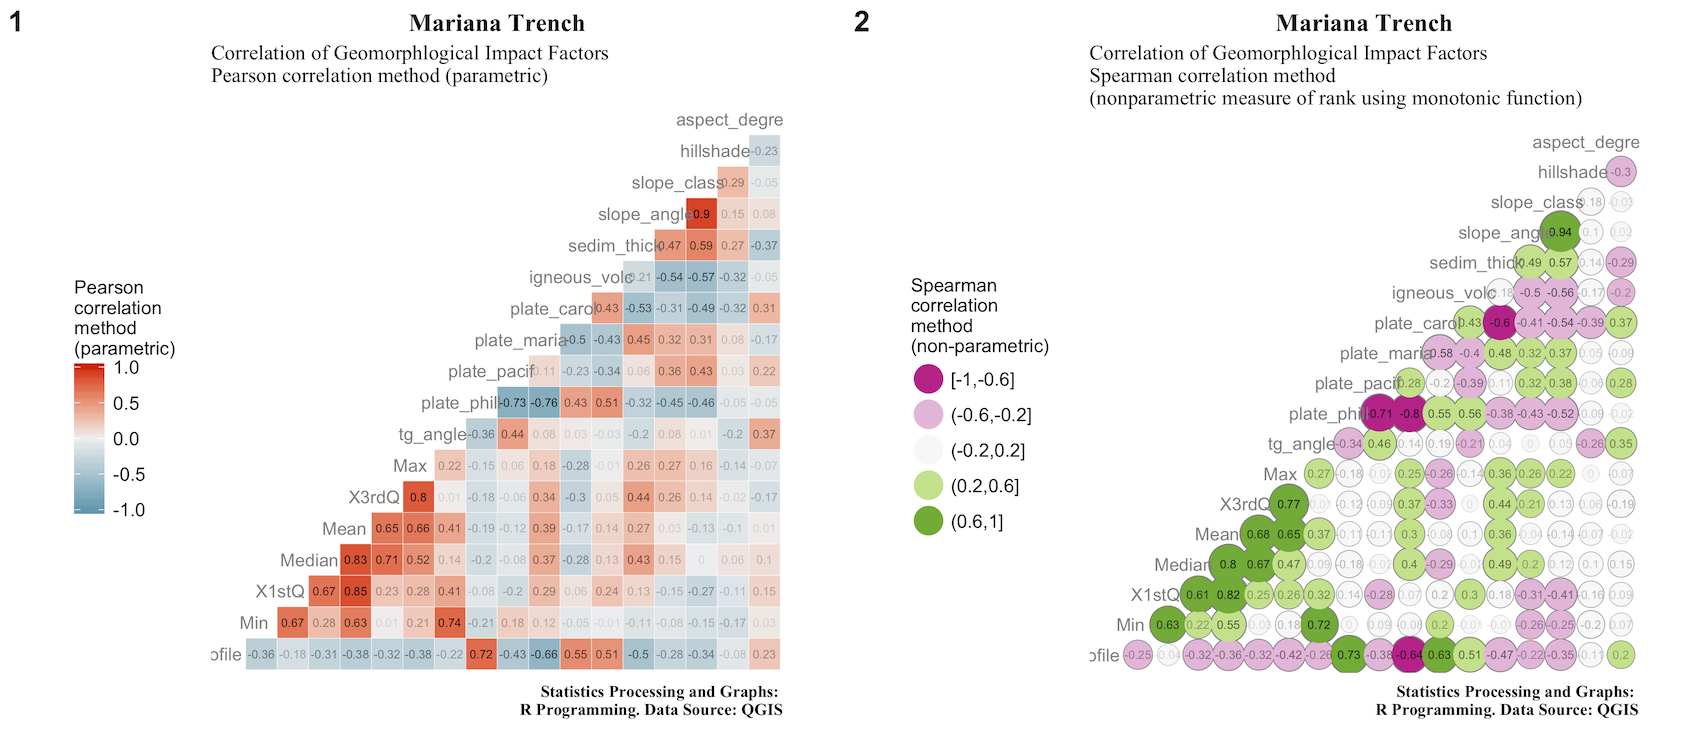
\includegraphics[width=13cm]{Fig-4-56.jpg}
	\caption{Pearson correlation for the Mariana Trench geomorphological impact factors (left). \\Spearman $\rho$ correlation ranking for Mariana Trench geomorphological impact factors (right).\\Computed in R by code: \ref{R:41}}\label{fig:4-56}
\end{figure}

On the Fig.\ref{fig:4-56} the more correlated variables are represented by the colors of green. The size of the circle also depends on the correlation value. Spearman’s rank correlation coefficient is denoted by $\displaystyle \rho$ or $r_s$. It is given by the following formula \cite{MyersWell2003}:\\
	\begin{equation}
		  r_s=1-\frac{6\displaystyle\sum({d_{i}}^2)}{n({n}^2-1)}
	\end{equation}\label{eq:7}\myequations{Spearman’s $\rho$ rank correlation coefficient}
	where\\
$d_{i}$ = rg ⁡($X_i$) − rg ⁡ ($X_y$) is the difference between the two ranks of each observation,\\
 n is the number of observations.\\
 
Here $d_{i}$ represents the difference in the ranks given to the values of the variable for each item of the particular data The formula of Spearman’s rank correlation coefficient $\rho$ is applied in cases when there are no tied ranks. Technically, the R programming script for Pearson correlation was changed in case of Spearman's $\rho$ by calling following code: \ref{R:41}. On Fig.\ref{fig:4-56} the measure of rank correlation, that is a statistical dependence between the rankings of two environmental variables has been computed using (GGalt) library by R code: \ref{R:41}. Spearman correlation shows (Fig.\ref{fig:4-56}) how well the relationship between every pair of two environmental variables can be described using a monotonic function and comparing following factors: tectonics, geology, geographic, bathymetric and magmatism. In other words, Spearman's correlation assesses monotonic relationships, whether linear or not between the bunch of available factors. If there are no repeated data values, a perfect Spearman correlation of +1 or −1 occurs when each of the variables is a perfect monotone function of the other.

	\subsubsection{Computing Kendall $\tau$ coefficient}\label{sssec:Kend}
	Alike to Spearman coefficient, Kendall $\tau$ coefficient to measure rank correlation, invented by Maurice Kendall, is also a non-parametric test for statistical dependence between environmental ordinal (or rank-transformed) variables. Kendall rank correlation distance is defined as follow:
	\begin{equation}
		  \tau=\frac{2}{n(n-1)}\displaystyle\sum sgn(x_{i}-x_{j})sgn(y_{i}-y_{j})
	\end{equation}\label{eq:8}\myequations{Kendall $\tau$ correlation coefficient}
	
Kendall rank correlation $\tau$ coefficient is a statistically used to measure the ordinal association between two measured quantities, that is environmental factors in this case. Based on the $\tau$ coefficient test, a non-parametric hypothesis test for statistical dependence has been computed by R code \ref{R:41}. It measures a rank correlation: the similarity of the orderings of the data when ranked by each of the quantities. Technically, the script for computing Kendall correlation. Similar to Spearman coefficient, but unlike Spearman's, can handle ties. Moreover, there are three Kendall $\tau$ statistics: $\tau$-a, $\tau$-b, and $\tau$-c, of which $\tau$-b is specifically adapted to handle ties. The $\tau$-b statistic handles ties, i.e., each pair of members of the environmental variables, e.g. tectonics and geological factors, or geographic location and magmatism, or sedimental thickness layer versus closeness of the igneous volcanic spots, – will have the same ordinal value by a divisor term. The latter represents the geometric mean between the number of environmental factor pairs that are not tied on factor one and the number not tied on two. Visualized Kendall $\tau$-correlation (Fig. 7) for geomorphological impact factors of the Mariana Trench and numerical scatterplot matrix (Fig. 8) are computed in R by code: \ref{R:41}, \cite{Lemenkova201871}. Numerical scatterplot matrix of correlation of the impact factors and cross-correlation matrix of the depth values in bathymetric profiles of the Mariana Trench (Fig. 9, \cite{Lemenkova201871}) are drawn using R scripting libraries: \ref{R:07}

	\subsection{\ac{PCA}}\label{ssec:PCA}
The \ac{PCA} (Fig. 10, \cite{Lemenkova201871}) performed using R code \ref{R:08} enabled to visualize eigenvectors as showing major direction and vector length for the principal components affecting the categorical values. Through the \ac{PCA} a statistical procedure using an orthogonal transformation to convert a set of bathymetric depth observations of possibly correlated variables, has been performed. Thus, the direction of the eigenvectors shows the depth of the Mariana Trench has been highly influenced by its geomorphic settings, particularly its location, by 25 profiles, as well as the similarities between the profiles.

	\subsection{Hierarchical cluster analysis for the data patterns recognition}\label{ssec:HCA}
	In the current research, the main method of the determining clusters of the environmental variables affecting Mariana trench formation is an algorithm provided by cluster analysis, executed by (dendextend) R library using code \ref{R:06}. Initially, the \ac{GIS} based digitizing of the 25 bathymetric profiles across the trench has been performed in \ac{QGIS}. The length of each profile was taken 1000 km, and the distance between every pair was 100 km. The coordinated were saved in a table with three columns: elevations, latitude and longitude. After that, R enabled to stepwise perform cluster analysis, data partition, sorting and grouping. Comparative analysis of the multi-dimensional data enabled to analyze inter-relationships between the factors impacting changes in the morphology and dynamics of the system of the trench. The most efficient method was computing hierarchical dendrogram clustering with p-values called by R library (dendextend). The default hierarchical clustering method used in this library is “hclust”. 
	
\begin{figure}[H]
	\centering
		\subfloat {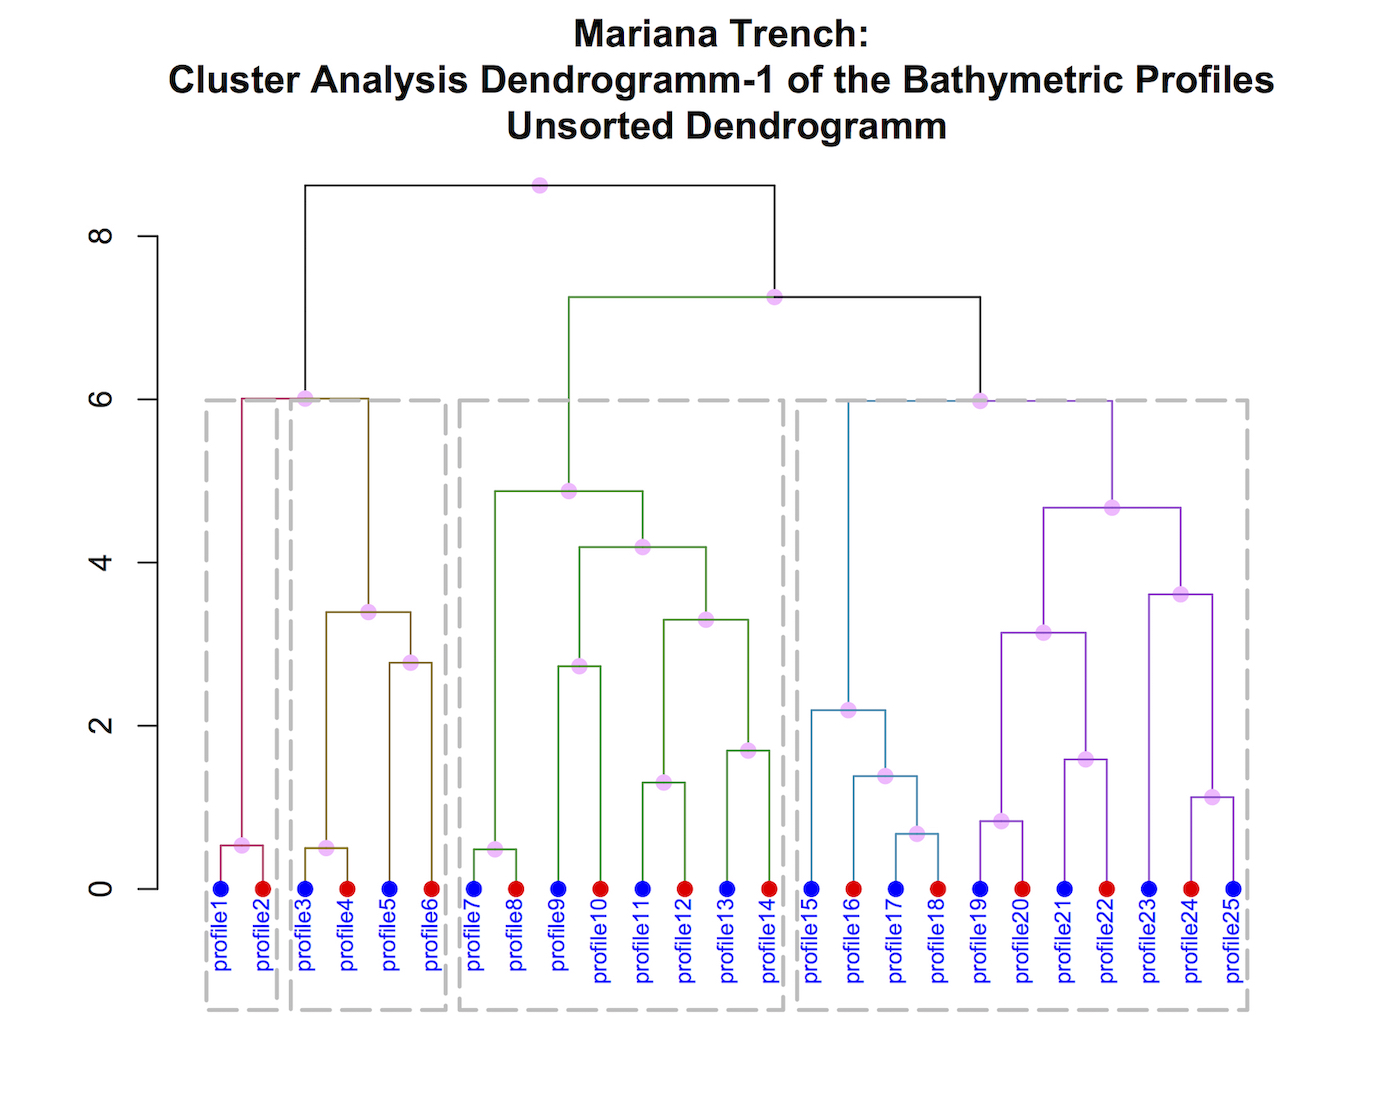
\includegraphics[scale=0.17]{Fig-4-3-8a.jpg}}
			\hspace{5mm}
		\subfloat {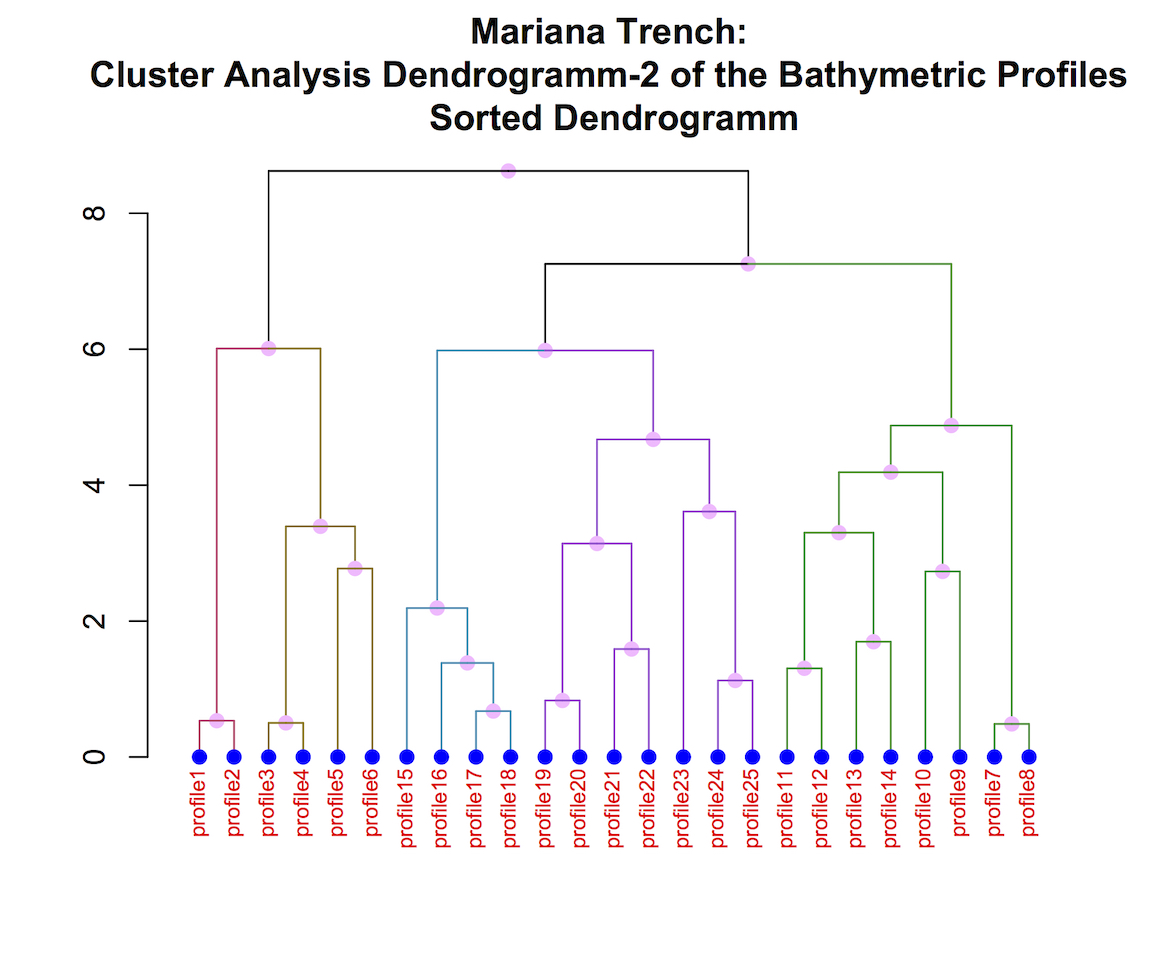
\includegraphics[scale=0.17]{Fig-4-3-8b.jpg}}
	\caption{R based dendrogram tree of the 25 profiles. Left: unsorted, right: sorted. Computed in R by code: \ref{R:06}}\label{fig:4-3-8ab}
\end{figure}

	The results of the executed algorithm have been visualized as a plotted dendrogram. The working flowchart include following steps: creating unsorted and sorted dendrograms (Fig. \ref{fig:4-3-8ab}), cross-comparison of the both, hierarchical clustering using p-Values, and dendrogram by clustering using bootstrap probability method (Fig. \ref{fig:4-3-8de}). The initial step included created unsorted dendrogram. Several adjustments have been made thereafter: changed and colored labels based on real profiles groups category, colored branches based on the procedure of cutting dendrogram tree into the clusters. Then the dendrogram was sorted using machine learning algorithm. After the reflection of the unsorted dendrogram on the sorted according to the data distribution by observation values, the model proceeded to the comparison of the two dendrograms (Fig. 4, \cite{Lemenkova201868}). The compared dendrograms now form cluster kernels. Further processing is completed on the machine by an embedded mathematical approach of R that filter out the less significant profiles and compares them to the kernel ones. The information is then stored to create final step: clustering using bootstrap probability method. Thus, there are four modifications of the initial model consisted of cross-section bathymetric profiles of the Mariana trench. The hierarchical dendrogram method was selected to test the data, due to its flexibility: this type of the machine learning is used specially for unlabelled data, i.e. without defined categories or groups, aimed to understand data possible allocation into groups. As the structure of the tectonics and trench geomorphic properties are rather complex, the dendrogram clustering facilitated data partition though defining the resulting groups, with similar morphology, distance to the volcanic areas, slope angles and sedimental thickness. The complete R programming script for cluster analysis is \ref{R:06}.	
	
\begin{figure}[H]
	\centering
		\subfloat {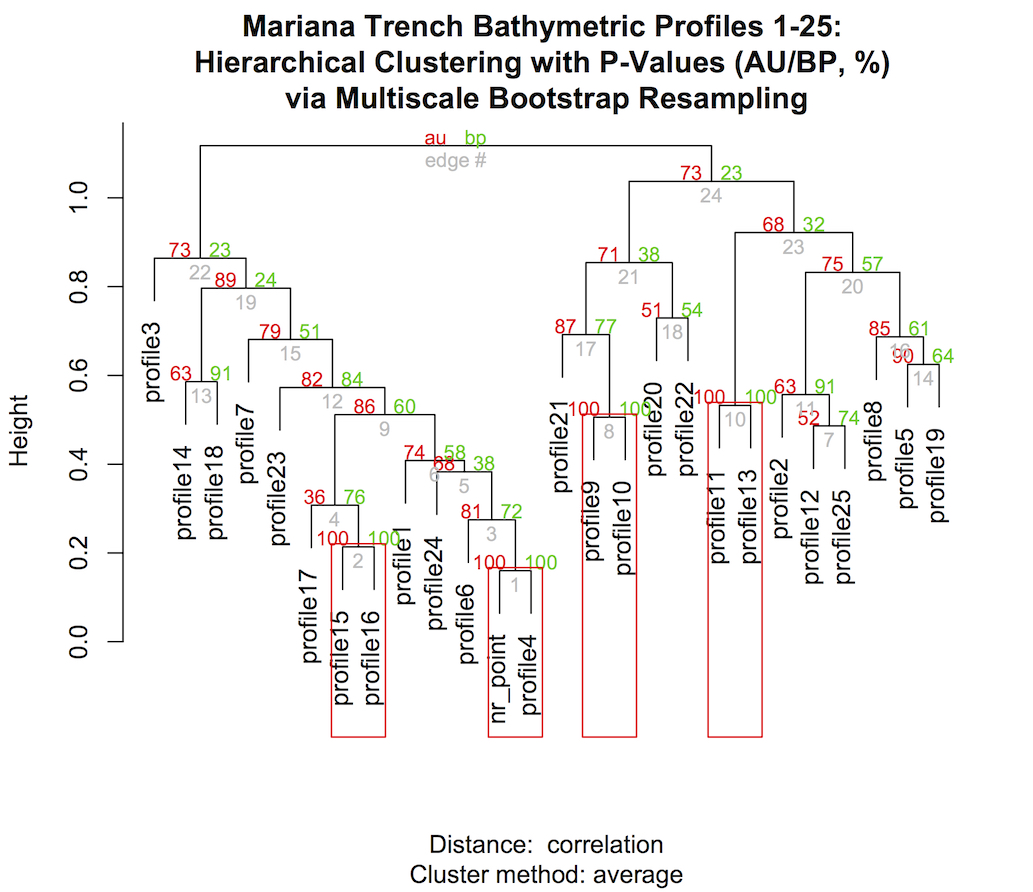
\includegraphics[scale=0.21]{Fig-4-3-8d.jpg}}
			\hspace{5mm}
		\subfloat {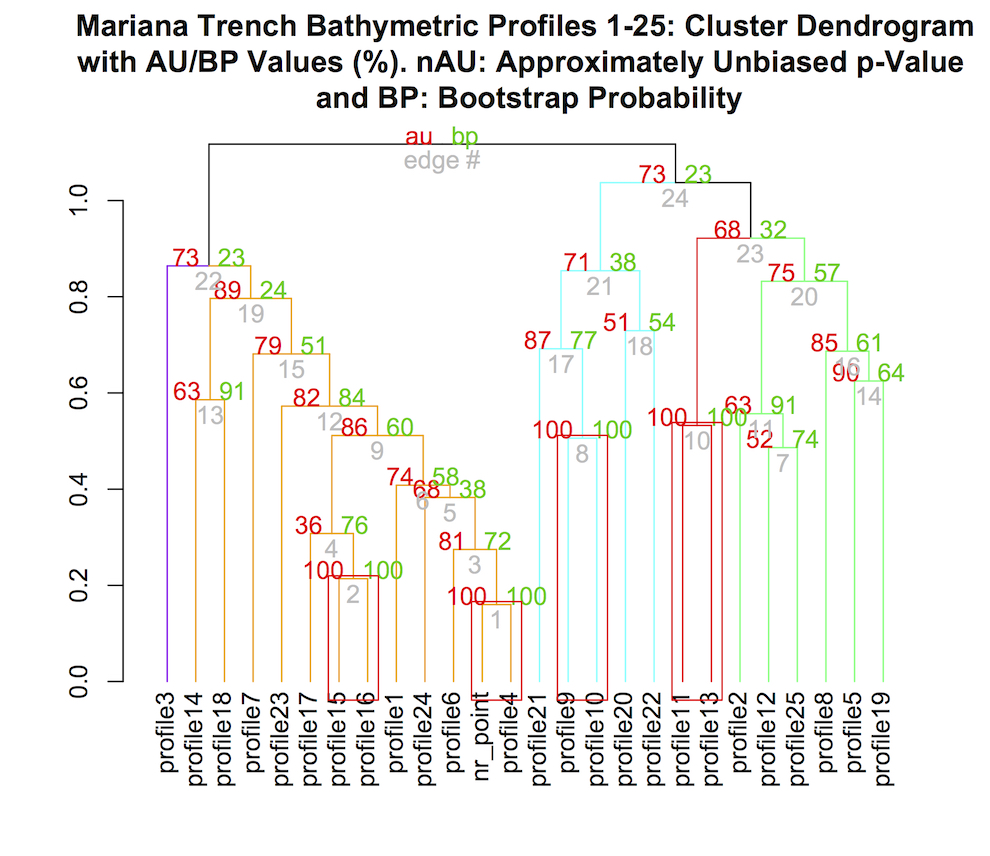
\includegraphics[scale=0.21]{Fig-4-3-8e.jpg}}
	\caption{Hierarchical clustering with p-values using multiscale bootstrap probability. Computed in R by code: \ref{R:06}}\label{fig:4-3-8de}
\end{figure}

	To summarize methodological application of this research, following conclusion can be drawn. The advantages consist in usability of many R libraries and algorithms at one time to understand the best option for the data set. When the proper method is found for each research step, the results are visualized as plot. In this case, the main method was dendrogram by the \{dendextend\} library aimed at data partition according to the environmental properties. As the programs received a table in (.csv) format and called script from the command line, it follows a mathematical algorithm to process the data. The R algorithm then calculated the values for the environmental values (geology, bathymetry, geomorphology, sedimentation and tectonics), and divided the dataset into clusters, according to the similarity of their values. Once the data are analyzed by the machine, the visualization of the bathymetric groups and data partition were successfully performed.

\subsection{Scatterplot Matrices}\label{ssec:SM}
Scatterplot matrices, also known as determinant for linear correlation between the multiple variables, are an efficient way to highlight the environmental variables that might have similar correlations to the geomorphic structure of the ocean trench. The scatterplot matrix is used to solve the problem of selection of the crucial impact factors affecting the hadal formation. The application is supported by purely practical algorithms of data partition that is, inspection of the possible determinants. The data with multiple variables congregating a geo-system are particular suitable to be used for the scatterplot matrix. The matrices correlation for four tectonic plates were executed by called using \{Ggally\}, \{data.table\} and \{ggplot2\} libraries. The following R programming script has been used to assess correlation between factors affecting Mariana Trench geomorphology: \ref{R:41}. The bathymetric determinant of the four distinct groups of the cross section profiles cause certain variability in the sedimental thickness of the basement, slope angle steepness degree, angle aspect, depth at the basement, as well as depth values (means, median and absolute minimum). Among other factors a magmatism of the nearby area is to be mention. The closeness of the igneous volcanic areas contribute towards earthquake frequency across four tectonic plates – Mariana, Pacific, Philippine Sea and Caroline. The results demonstrated that cross-section profiles of the Mariana Trench can be divided into clusters according to their properties, such as bathymetric (depth values), geographic (latitude and longitude), geological (width of the sedimental thickness layer), magmatism (large igneous polygon areas) and tectonic (location of the tectonic plates nearby).\\
In the scope of current research a functionality of R programming language has been tested. It proved to be as an effective tool for studying distribution of the environmental factors affecting the tectonic structure, as well as geomorphic properties at the seafloor basement of the Mariana Trench. Using scatterplot matrices, the distinct unevenness of various factors affecting Mariana Trench geomorphic structure can bee visualized \cite{Lemenkova201901}. In general, the algorithms of the plotting scatterplot matrices consist of taking the values of the variables to show correlation of their values with others across the range of the data set. It is expected to show similarity at diagonal view, with increasing dissimilarity as the differences in the geologic and tectonic values increases. Scatterplot matrices analyzing correlation between environmental factors have the following correlation characteristic: the correlation function shows similarities between the characteristics of the four tectonic plates: Philippine, Mariana, Caroline and Pacific. When the time bathymetric values increases (Fig. 1, \cite{Lemenkova201901}, right center), the correlation with sediment thickness increases to a maximum. \\
	As the observation points change their position from plates by sample points, the correlation again increases back to a maximum, because the characteristics of the geology change by geographic location. The notable peak in the correlation between the magmatism of the close igneous volcanic areas and slope angle degree indicates the dependancies between the geomorphology and tectonic properties. The method of the scatterplot matrices shows appropriate visualization for the large data set overstepping thousands of the observation points. The scatterplot matrices were plotted using functionality of R \cite{RCoreTeam2014}.\\
	The scatterplot matrix displays values for typically the environmental variables for a set of data that include depths, aspect and slope angles of the bathymetric profiles, sediment thickness, closeness of the volcanic areas and the topographic settings (maximal and mean depth values, by profiles). The diagonal view of the scatterplot matrix gives an inside in to the relationships between these factors. Based on the scatterplot matrix it can be roughly determined that there is a linear correlation between several environmental variables constituting the project of the Mariana Trench: sediment thickness have similar correlations to the slope angle degree and a depth values. Scatterplot matrix is one more advantageous approach for the analysis of the big data sets containing multi-source data. \\
	The inter-relationships and links between the sediment thickness, slope angle steepness and depth of the bathymetric profiles cross-sectioning Mariana Trench are shown on (Fig. \ref{fig:COMU-9}. The sediment thickness gives a response towards the steepness of the angle and the depth. The rate of the submarine sediment accumulation is critical due to the preconditioning by the mentioned above factors. It is also highly sensitive to different triggering factors, such as ocean deep currents that contribute towards the hadal sedimentation, as well as accounting for the topographic variability observed in the cross-section profiles.\\
	More importantly is that the effects of those triggering factors that increase sedimentation (that is location of the profile, crossing four tectonic plates and steepness of the angle) may hidden other environmental triggers underlying the sedimentation responses induced, for instance, by the biomass accumulation in the deep layers of the trench. Changes in the patters of the deep current direction s and intensity brought on by triggering factors, e.g. submarine volcanism, may cause an increase of sedimentation proving a feedback mechanism between the marine geological and biological factors. The evidence of such feedback mechanism should be observed as a recommendation for the further studies based on the available data derived from the cruise observations. The submarine sedimentation in the hadal trenches spatially correlate not only to the geological and tectonic factors of the specific trench, but also to the deformation features at the trench that induce submarine volcanism and closeness of the igneous volcanic areas. In such cases, the sedimentation response to such factors is a rapid process. Scatterplot combined matrix that enables to visualize several approaches on one matrix (Fig. \ref{fig:COMU-11}): scatter plots, box plots with residuals, margin plots and surface plots, R code \ref{R:41}.

\begin{figure}[H]
	\centering
		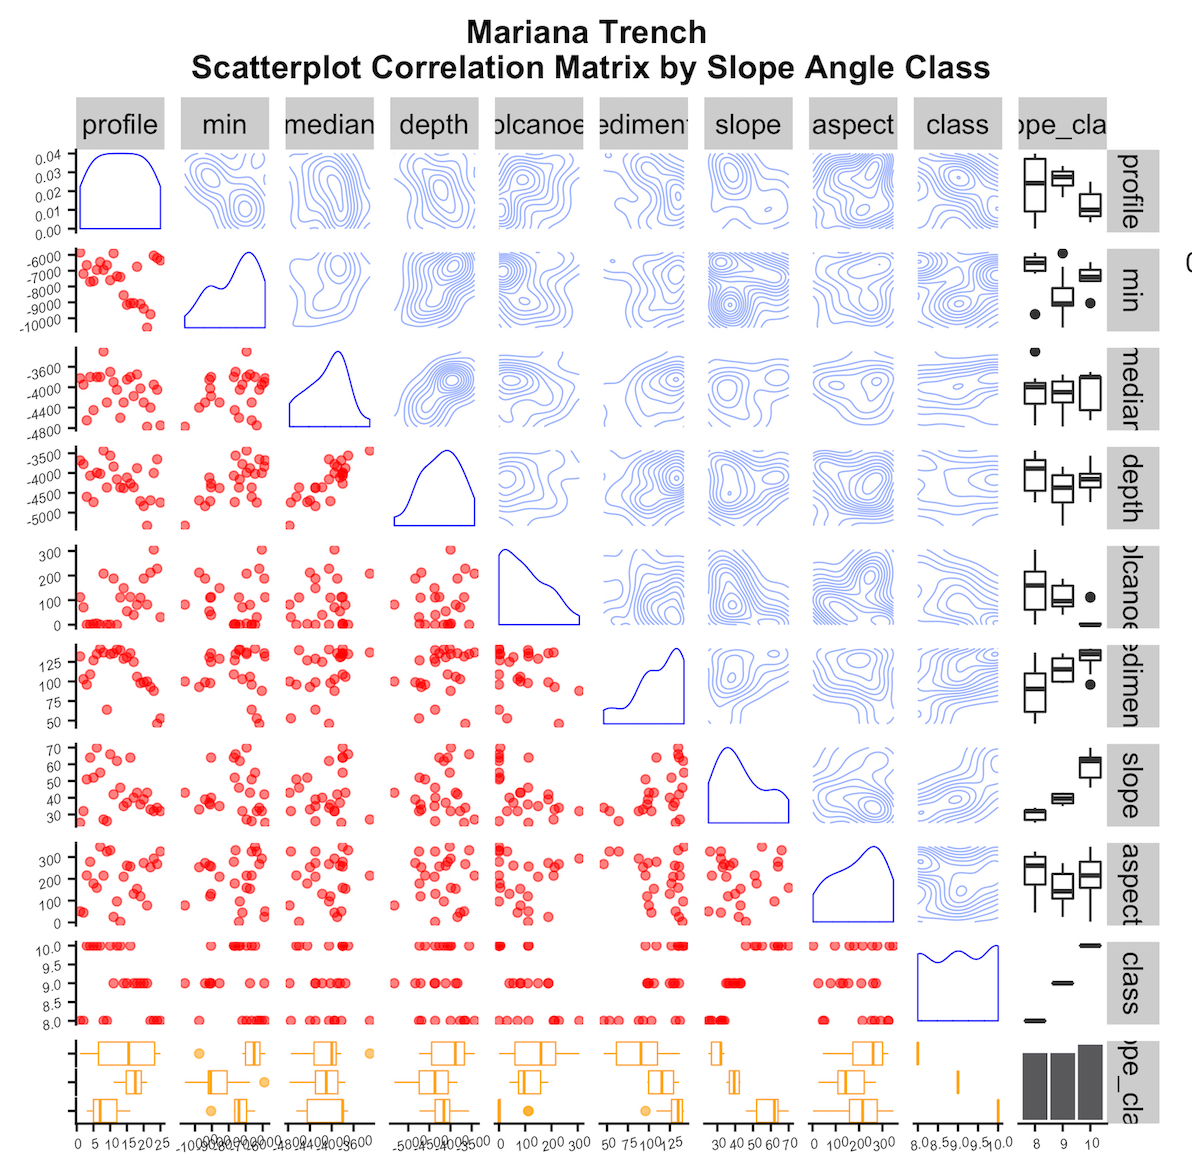
\includegraphics[width=8cm,clip]{Fig-COMU-11.jpg}
	\caption{Scatterplot matrix: correlation between the variables. Plotting: R.}\label{fig:COMU-11}
\end{figure}

The results indicate (Figure \ref{fig:COMU-11}) that sediment sources at the Mariana Trench are connected with trench tectonics. This part of the research uses the statistical approaches to analysis a large dataset (12.950 observations taken from the attribute tables) using Python and R. The application of statistical algorithms embedded into programming languages towards studies in marine geology proved to be and effective tool for data analysis. 
	
\subsection{\ac{EFA}}\label{ssec:EFA}
This factor analysis and  \ac{PCA} are based on \citep{Lemenkova201866} using R script: \ref{R:26}. The R libraries for scripting simulations were used to model principal factors affecting the morphology of the trench. For the factor analysis the entire modeling process including grid generation, model setup, execution and analysis of the results with visualized correlation matrix showing the more important factors impacts according to their values, has been carried out from a single R script, with the results of the correlation matrix shown on Fig. 4 \cite{Lemenkova201866}). The standardized loadings based upon correlation matrix of factor analysis of the Mariana Trench (Fig. 5 \cite{Lemenkova201866}) show the impact values of each factor. 

For this research the fa() function from R was used (\ref{R:26}), which received the following primary arguments: r: the correlation matrix; Nfactors: number of factors to be extracted; rotate: one of several matrix rotation methods, such as “varimax” or “oblimin”. \\
Next, an alternative to factor for the components analysis was performed using \{FactoMiner\} library by cluster analysis iCLUST (Fig. \ref{fig:4-3-9ef}). This goal is the same as factor or components analysis, but methodologically, it reduces the complexity of the data and attempts to identify homogeneous sub-groups. Here, the exploratory factor analysis aims to extract a more regular impact factors of the geologic morphology development, whereas cluster analysis and hierarchical dendrogram extract the groups and classes in a total cloud of the bathymetric observation points. Finally the factor analysis results in the illustrating cross-influences of the most notable factors: geological, geomorphological, tectonic, geographic and environmental parameters. This enabled to quantitatively analyze correlation between the actual shape of the trench and its environmental impact factors (Fig. 6 \cite{Lemenkova201866}). Fm: one of several factoring methods, such as “pa” (principal axis) or “ml” (maximum likelihood), as shown on the code: \ref{R:26}. \\
The $\omega$ testing was done to find out two alternative estimates of the reliability that take into account the hierarchical structure of the inventory data are $\omega$ (Fig. \ref{fig:4-3-9gh}). These were called using the omega function for factor analysis, R: \ref{R:26}. The computed coefficient omega (hierarchical) ($\omega$ h) is an estimate of the general factor saturation of the performed test. Various factoring methods have been tested in this research to better describe data factors. Nevertheless, the fa() function provided the best results used for common factoring (Fig. 7 \cite{Lemenkova201866}). In this research the oblique rotation (rotate = “oblimin”) has been used, which recognizes that there is likely to be some correlation between geomorphological factors affecting Mariana Trench formation. The principal axis factoring (fm = “pa”) was used in this research, as the identifying the underlying constructs in the data was not necessary in this case. The \ac{EFA} matrix is shown on Fig. \ref{fig:4-3-ref}. \\
Once all the cross-section profiles had been inspected, the assessment of the bathymetric observation points and other environmental parameters (depth, sediment thickness) has been met by the factor analysis correlation matrix: Fig. \ref{fig:4-3-9ef}. The factor loadings (Fig. 5 in \citep{Lemenkova201866}) enable to assess the results of the factor solutions. Thus, we can see that the sediment thickness (factor solution = 0.65), slope angle steepness (factor solution = 0.61), and Mariana Plate location (factor solution = 0.74) have high factor loadings >0.5 around 0.7 on the first factor (PA1). 

\begin{figure}[H]
	\centering
		\subfloat {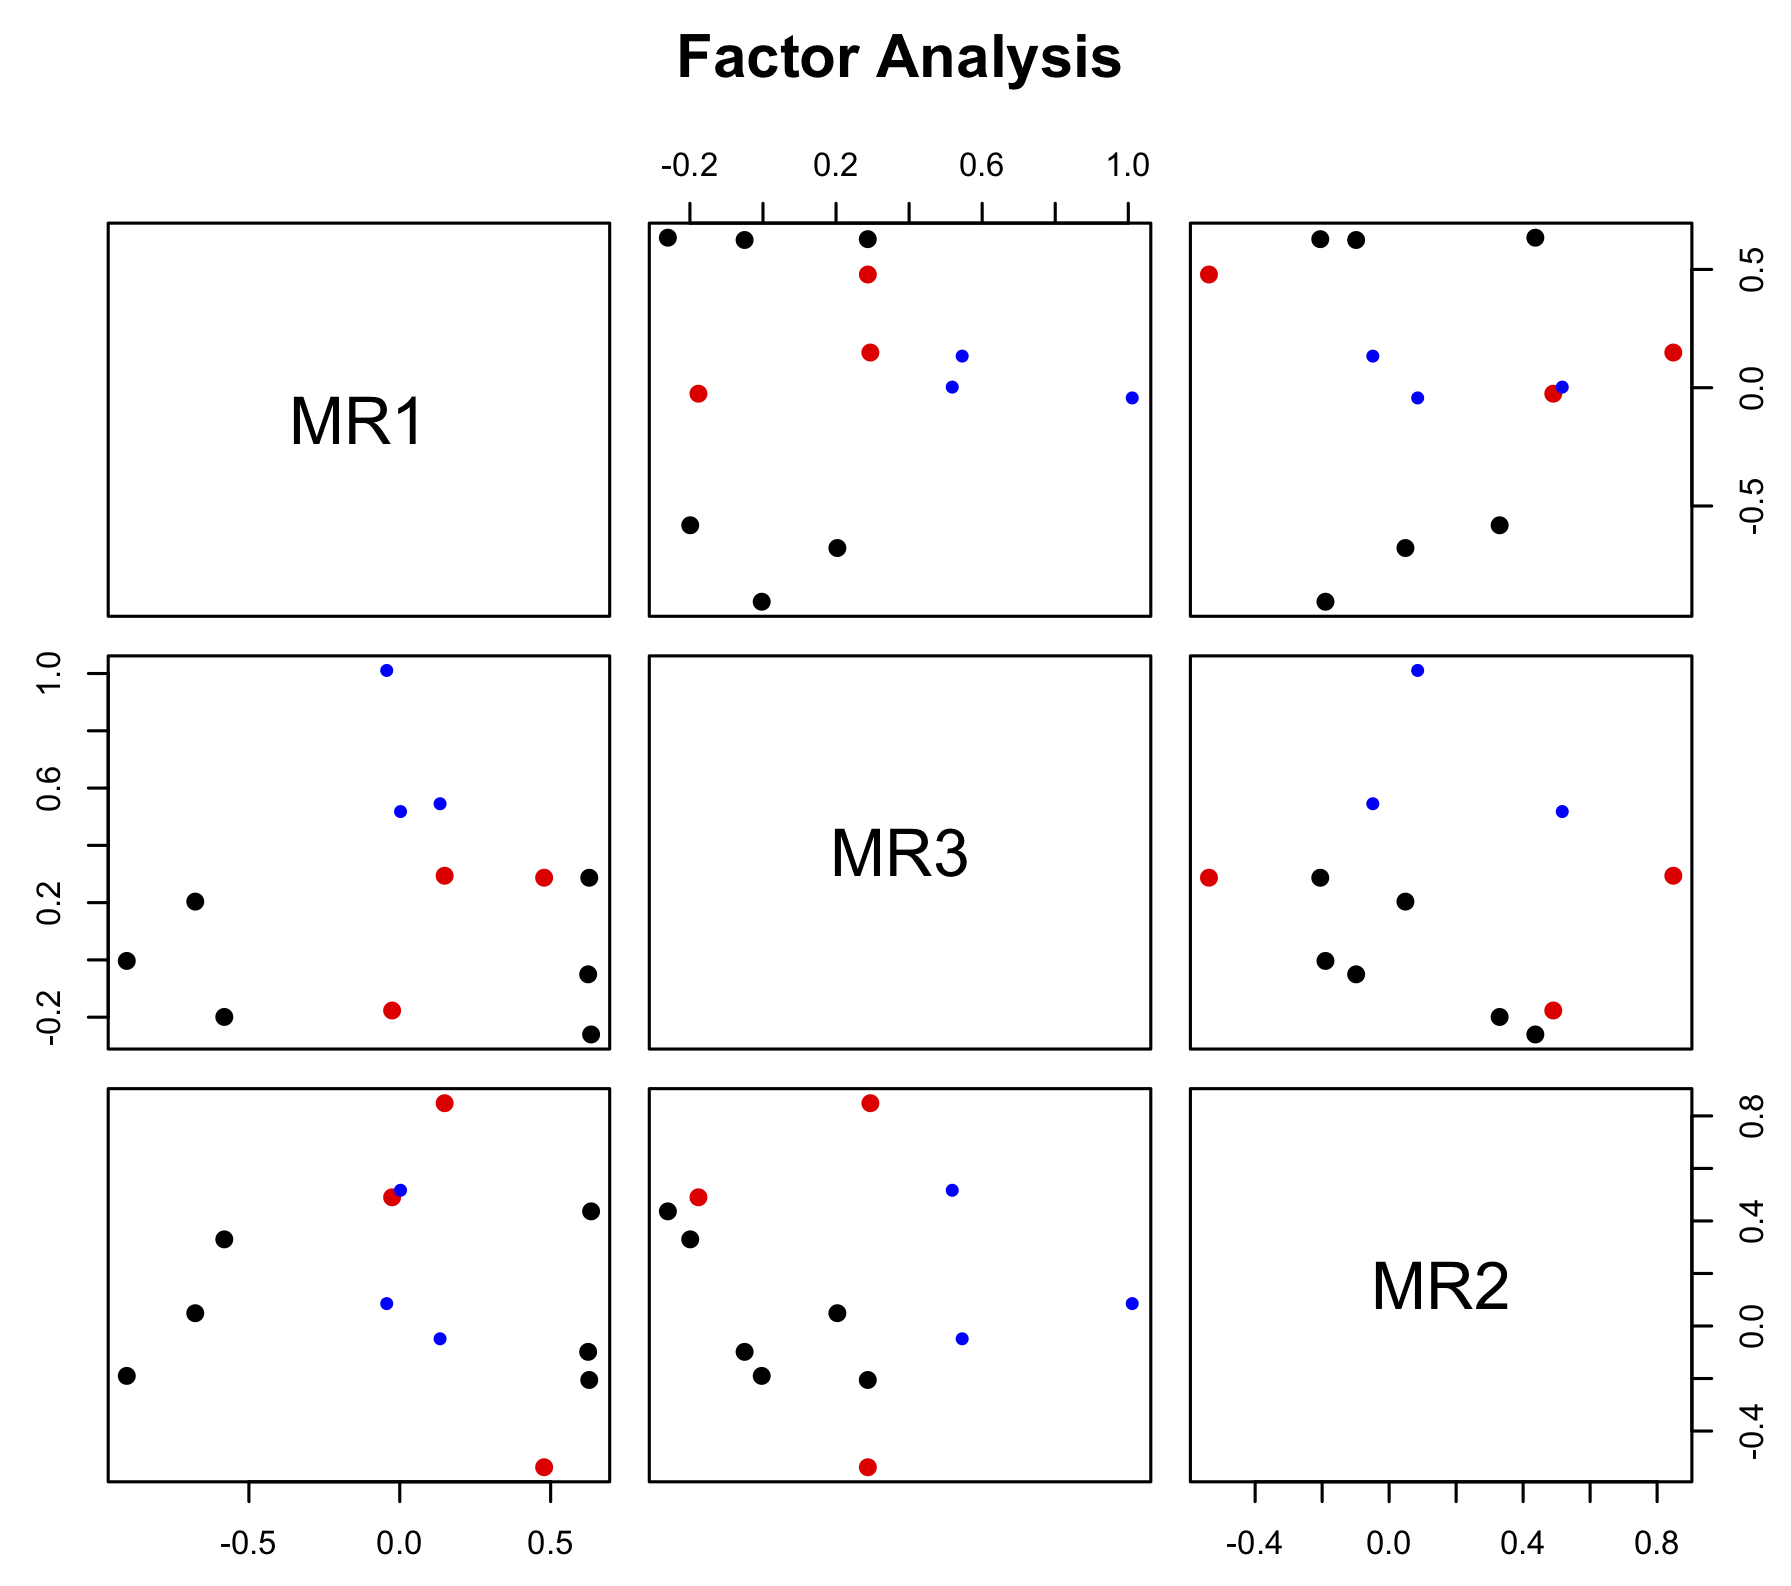
\includegraphics[width=8cm]{Fig-4-3-9e.jpg}}
			\hspace{5mm}
		\subfloat {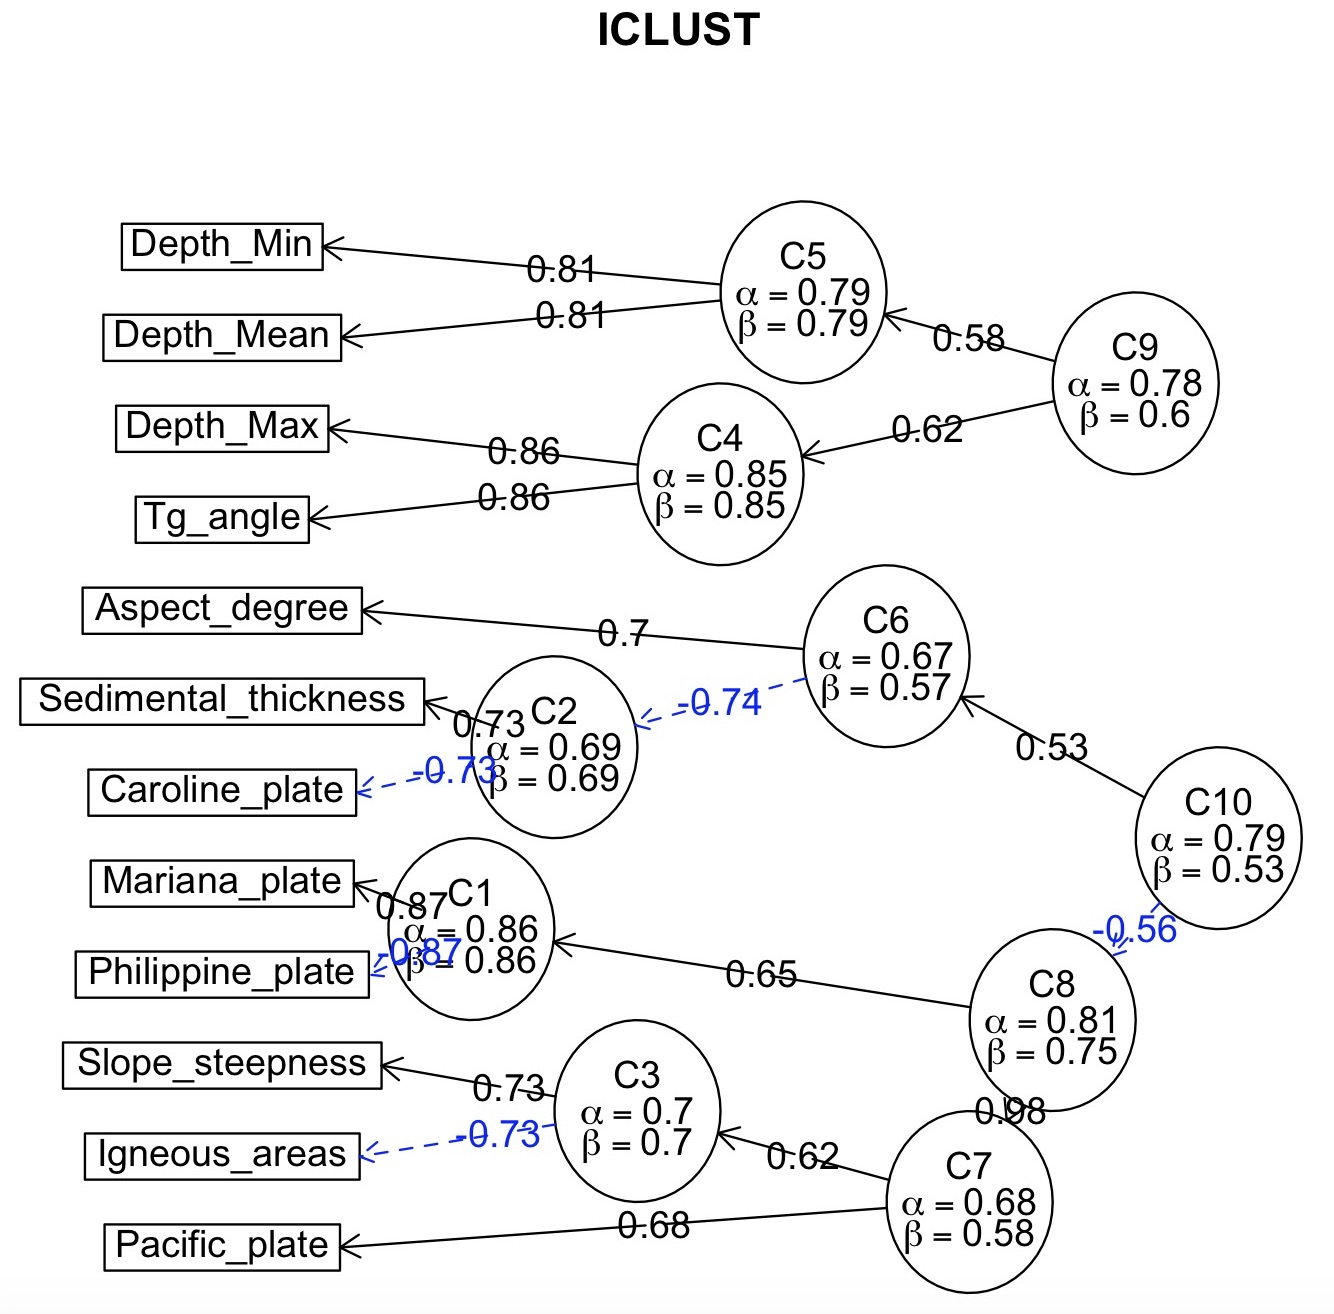
\includegraphics[width=7cm]{Fig-4-3-9f.jpg}}
	\caption{EFA correlation matrix (left). iCLUST analysis (right). \\Computed in R by code: \ref{R:26}}\label{fig:4-3-9ef}
\end{figure}

Therefore, these factors are the most influencing and representative for the morphology of the trench. The sediment thickness is mostly impacted by the slope steepness degree. Two geophysical indicators were particularly tested in the comparative analysis. It was furthermore found that slope degree and amplitude has important impact on the sediment thickness, while the aspect degree has lesser effect. Secondly, the second column (PA2) reveals (Fig. 5 \cite{Lemenkova201866}) that calculated tg \degree slope angle has a factor solution = 0.98 (extremely high), following by depth distribution (factor solution = 0.76). 
\begin{figure}[H]
	\centering
		\subfloat {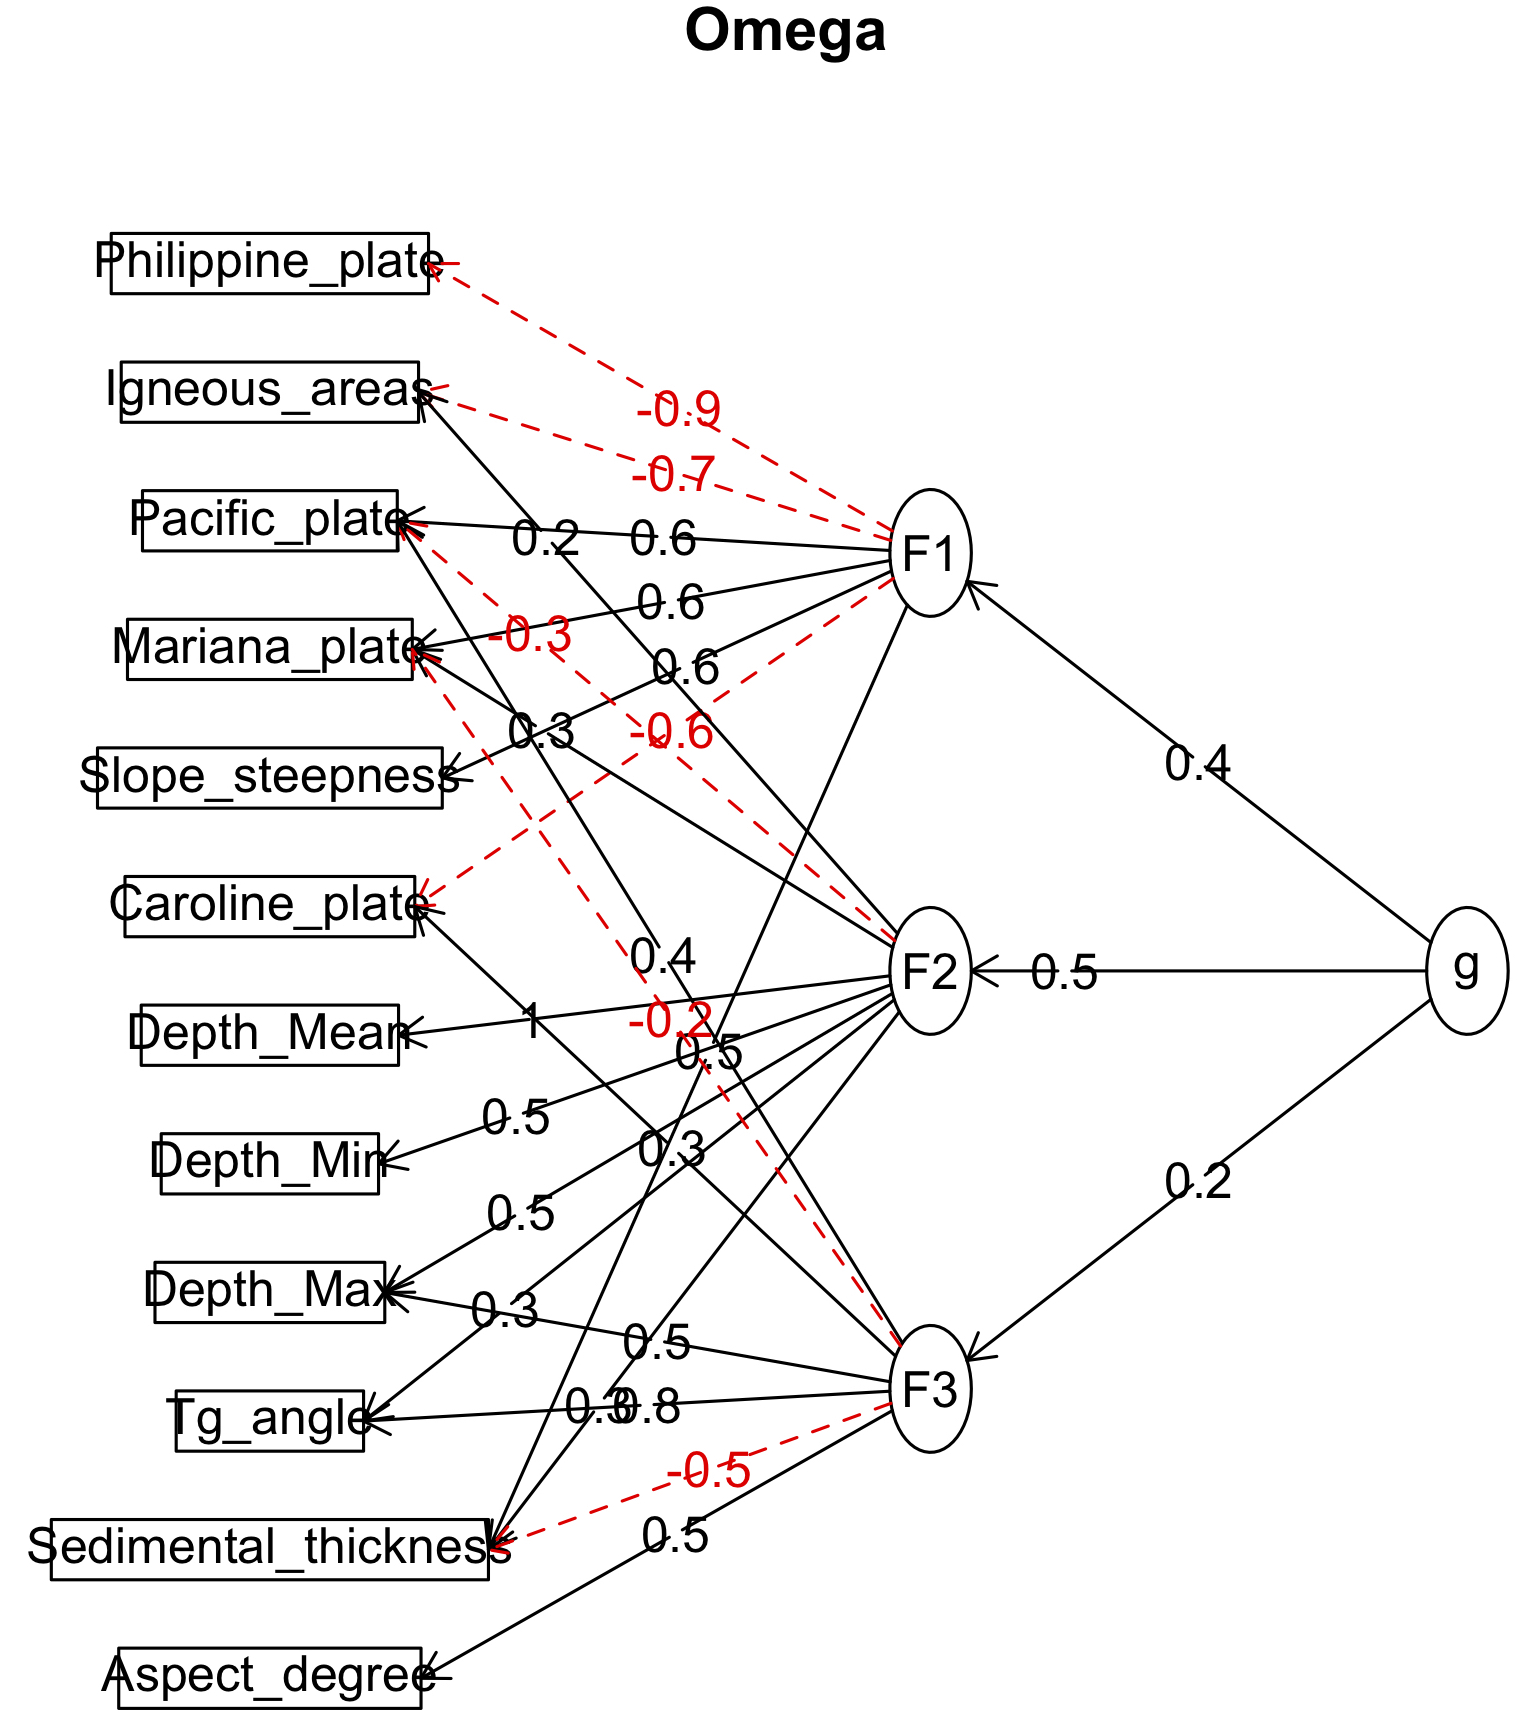
\includegraphics[width=7cm]{Fig-4-3-9g.jpg}}
			\hspace{5mm}
		\subfloat {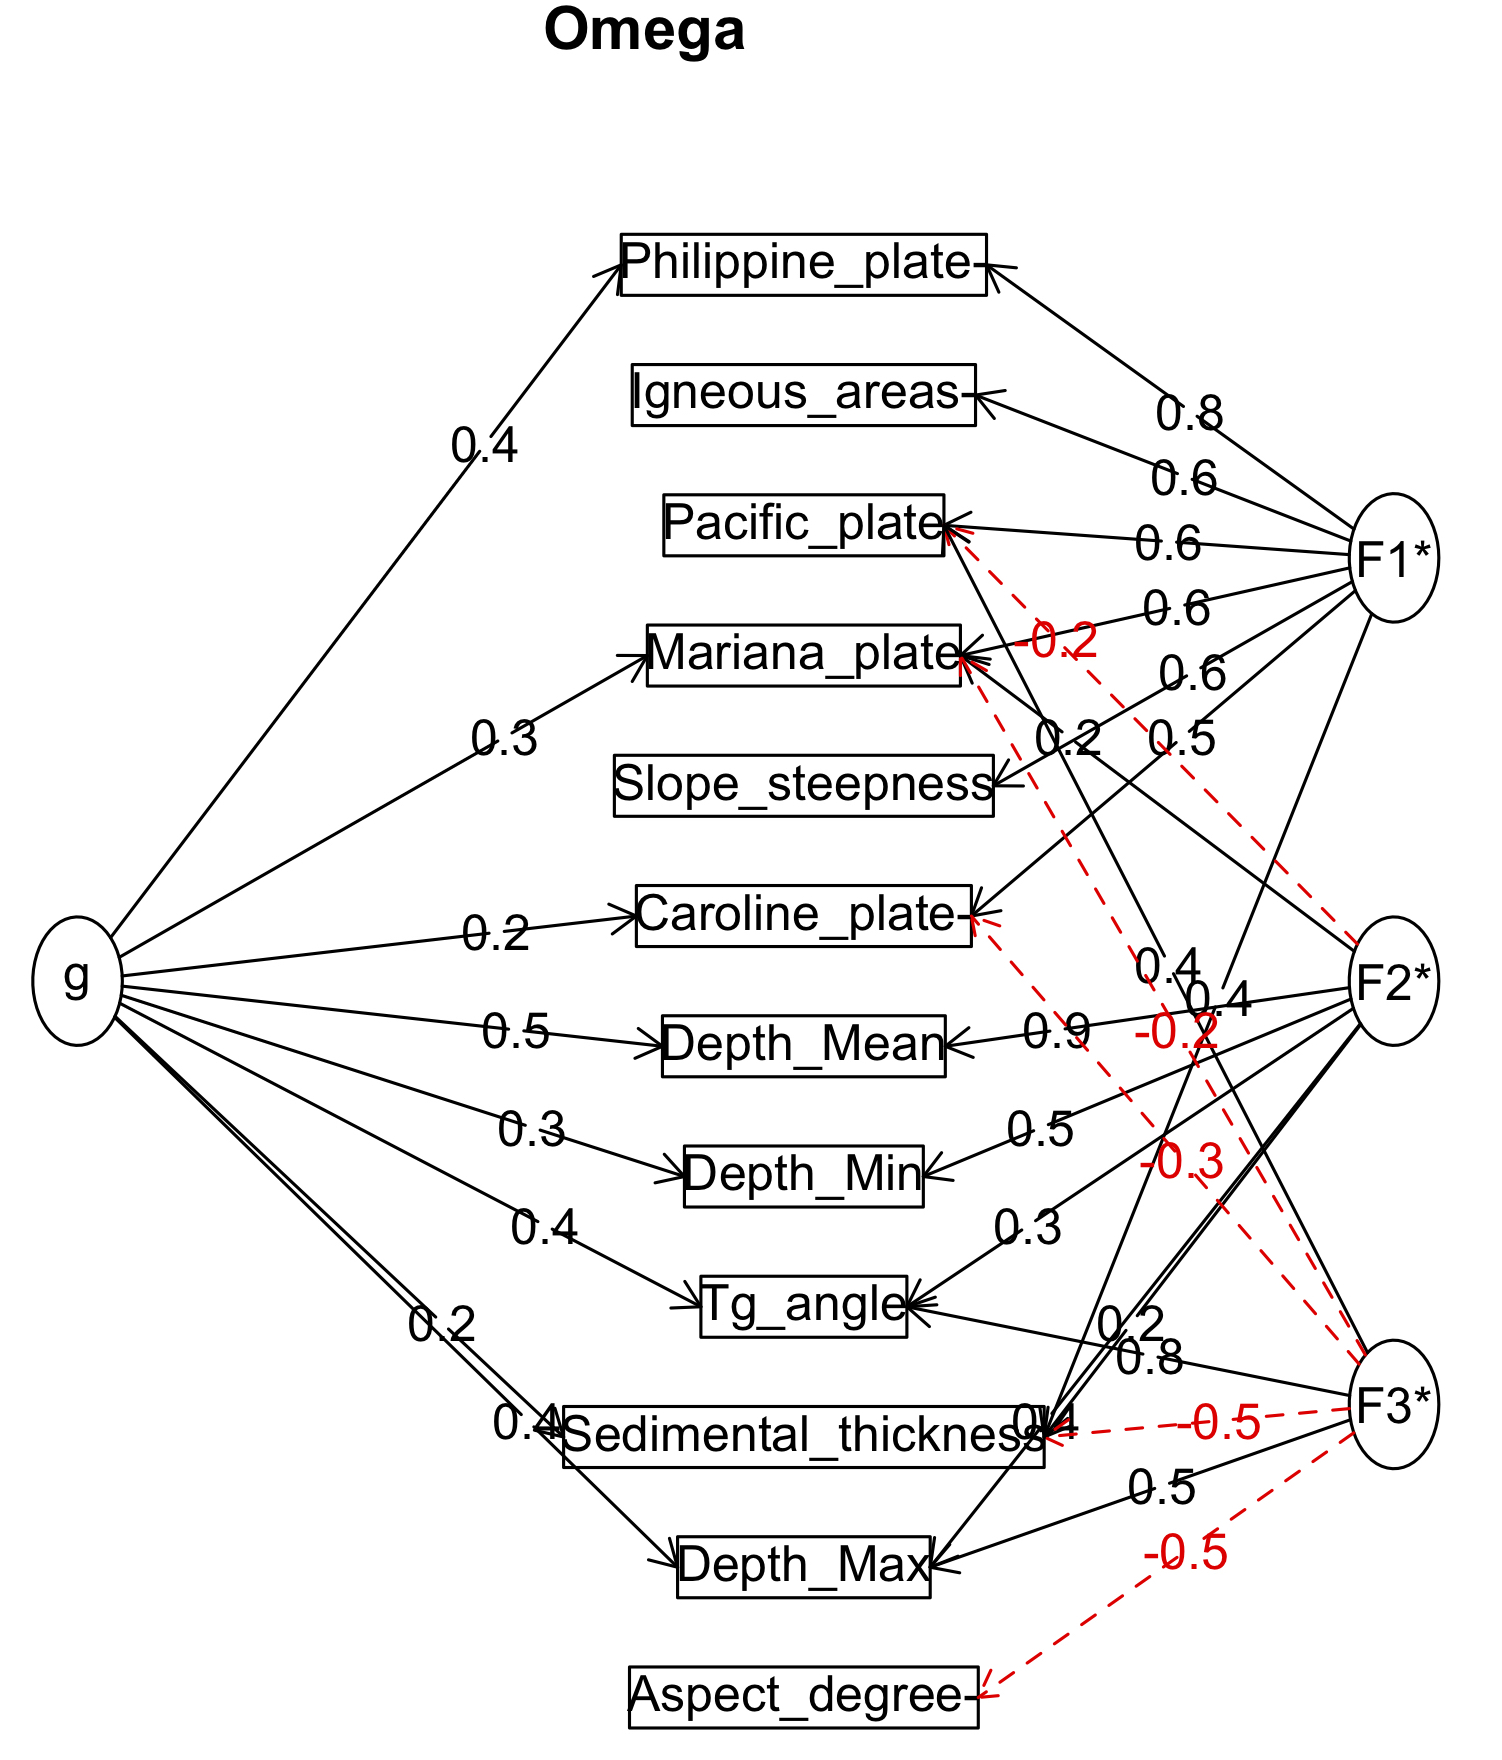
\includegraphics[width=7cm]{Fig-4-3-9h.jpg}}
	\caption{General factor saturation ($\omega$h) (left). General factor saturation through $\omega$ coefficient: 3 factors ($\omega$) (right). Computed in R by code: \ref{R:26}}\label{fig:4-3-9gh}
\end{figure}
The location of the Caroline and Philippine Plates do not affect that much Mariana Trench having negative factor solutions -0.79 and -0.70, respectively), as well as a much lower loading on PA2 (factor solutions = 0.25 and 0.12) and that it has a slight loading on factor PA1. This suggests that statistics is less related to the concept of Caroline and Philippine Plates than Mariana Plate and its geomorphic environmental settings, such as tg\degree slope angle, sediment thickness, slope angle steepness. Furthermore, on the resulting table (Fig. 5, \cite{Lemenkova201866}) one can see that each factor accounted for around 20\% (0.26\% and 0.18\%) of the variance in responses, leading to a factor solution that accounted for 100\% of the total variance (Cumulative proportion PA2: 1.00) in the Mariana Trench morphology formation. Finally, these factors are correlated in-between at 0.15 and recall that this choice of the oblique rotation allowed for the recognition of this relationship. The hypothesis testing was sufficient, with following factors having the highest score: tg\degree slope angle, sediment thickness, Mariana Plate location.
\pagebreak

	\subsection{\ac{ANOVA} to assess hypothesis testing}\label{ssec:ANO}
	The results have been interpreted on the homogeneity of variance by means of the one-way \ac{ANOVA} series of tests (Figure \ref{fig:ANOVA}). Several test methods were executed in this research. The brief description of their advantages and particularities is given below. The Tukey \ac{HSD} multiple pairwise-comparisons was applied to the \ac{ANOVA} results. Since the \ac{ANOVA} test is significant, the Tukey \ac{HSD} test was computed by R code: \ref{R:28}. TukeyHSD() takes the fitted \ac{ANOVA} as an argument. \begin{figure}[H]
	\centering
		\includegraphics[width=13cm]{Fig-ANOVA.jpg}
	\caption{ANOVA hypothesis testing. Computed and visualized in R code: \ref{R:28}}\label{fig:ANOVA}
\end{figure}
This test enabled to perform multiple pairwise-comparison between the means of groups. The library \{multcomp\} was used to perform a Pairewise t-test and to calculate pairwise comparisons between the group levels with the corrections for the multiple testing using R function pairewise.t.test(). The Levene’s test was used to analyse the homogeneity of variances at the next step of \ac{ANOVA} testing by calling function leveneTest() in the {car} package: \ref{R:28}. Comparing to the Pairewise t-test, the advantages of the Levene’s test is its lesser sensitiveness towards the departures from the normal distribution. Afterwards, the Welch test was executed in parallel to the oneway.test() in experimental mode. The Welch-test does not require that assumption have been implemented in the function oneway.test() which make is more suitable comparing to the last one. The Shapiro test was alternatively used to analyze variance of the residuals (Figure \ref{fig:ANOVA}). 
Finally, a non-parametric Kruskal-Wallis rank sum test was applied to finish with a series of \ac{ANOVA} testing. The result have been interpreted on homogeneity of variance by means of one-way \ac{ANOVA} tests. Since the p-value (Figure \ref{fig:ANOVA}) is less than the significance level 0.05, one can conclude that there are significant differences between the groups highlighted with “*" in the model summary, that is four tectonic plates: Philippine, Pacific, Mariana and Caroline. The Tukey multiple pairwise-comparisons test enabled to perform multiple pairwise-comparison between the means of groups and demonstrated 95\% family-wise confidence level of the results. The plotted homogeneity of variances of the results are shown in Figure \ref{fig:ANOVA}.

	\subsection{Euler-Venn Diagram}\label{ssec:EV}
Finally, the logical visualization of the results as Euler-Venn diagram (Fig. \ref{fig:4-3-10ab}) is created as a visual illustration of the most notable geomorphological parameters which enables to analyze correlations between the environmental factors affecting trench geomorphology. The Euler-Venn diagram shows 4 and 6 factors (Fig. \ref{fig:4-3-10ab}), respectively. It has been drawn to visualize all possible crossings between the variables using \{venn\} library of R calling following script: \ref{R:23}

\begin{figure}[H]
	\centering
		\subfloat {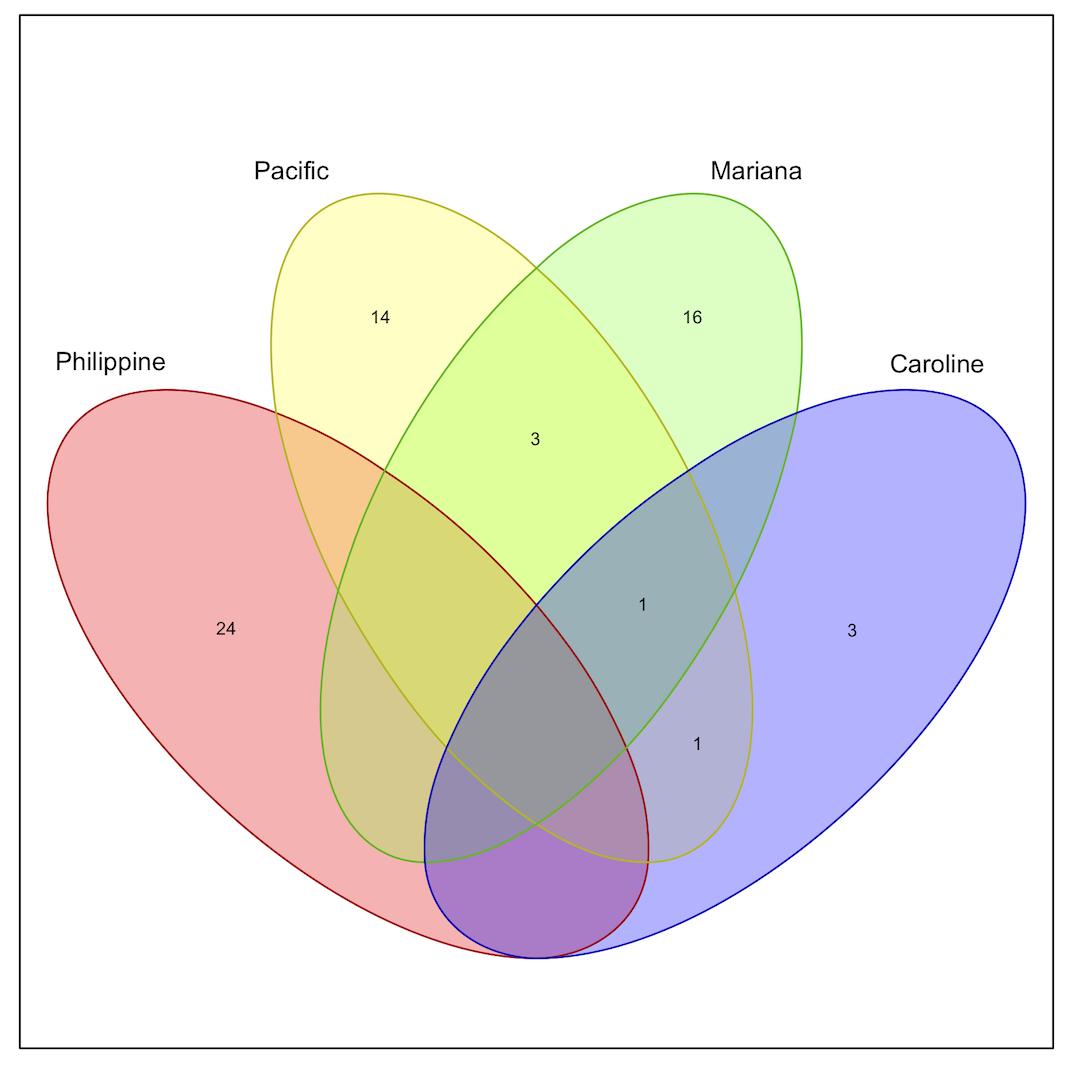
\includegraphics[width=7cm]{Fig-4-3-10a.jpg}}
			\hspace{3mm}
		\subfloat {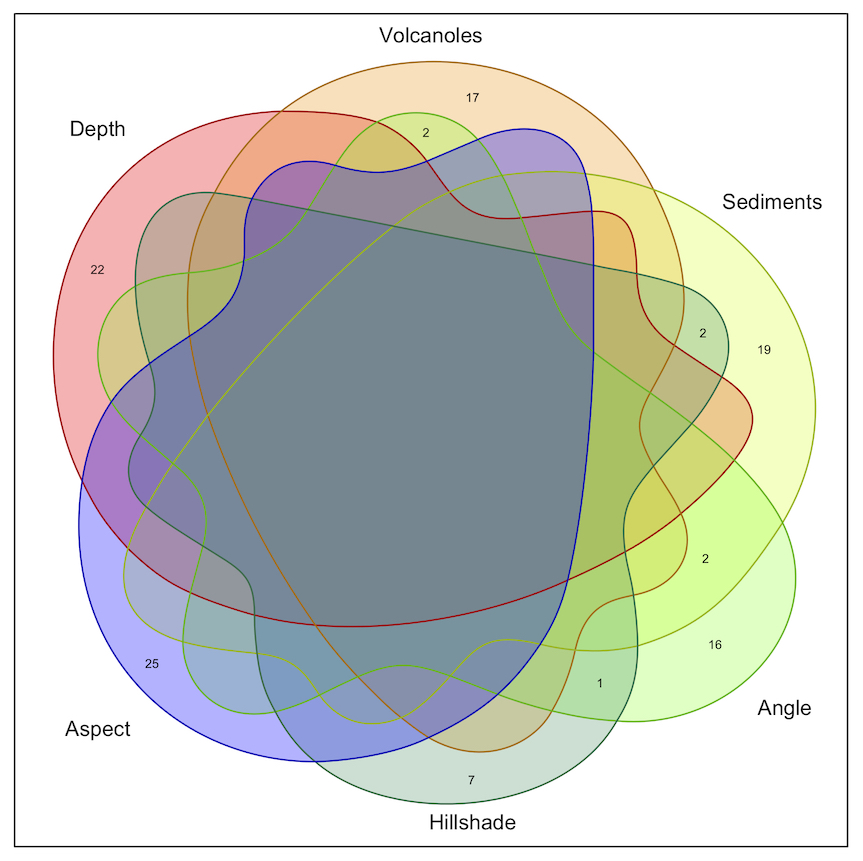
\includegraphics[width=7cm]{Fig-4-3-10b.jpg}}
			\hspace{3mm}
	\caption{Euler-Venn logical diagram on correlation of impact factors affecting Mariana Trench. Left: four tectonic plates. Right: environmental factors. Computed in R by code: \ref{R:23}}\label{fig:4-3-10ab}
\end{figure}

	\subsection{Hierarchical edge plotting and word cloud}\label{ssec:Hedge}
	Finally, the integrated use of GIS, statistical methods, R programming applied for geological data processing aimed at a multi-disciplinary approach to study spatial distribution of the impact factors affecting trench geomorphology schematically represented on Fig. 22 \cite{Lemenkova201991} by R code \ref{R:34}. The interpretation and classification of the geospatial data by R were useful for estimating impact factors and triggers of the development and structure of the geomorphological structure of trench. A visual grouping of all methods, approaches and data as a cumulated flowchart is presented on Fig. 22 \cite{Lemenkova201991} as a 'wordcloud' created by the \{wordcloud\} library via R code: \ref{R:36}.
\pagebreak
	
\section{Python language for marine geology}
\subsection{Why Python ?}

	Applying Python, a high-level programming language of general purpose, for marine geological data analysis and processing oceanographic data is still a novel approach. Usually applied and developed for \ac{IT} domain  applications, such as computer data analysis or data science, Python initially released in 1991 by \cite{Rossumatal2018} can effectively be applied in the marine geology. There are various significant advantages of the Python that make it a stand-alone language among the others. The advantages of Python can be summarized in a concise way in a Tab. \ref{tab:T10} as following answer to the main question of this subsection:
	The polymorphism embedded to the Python syntax enables to seamless overload standard operators to adjust their behavior in the context of the current task. Since Python is a very-high-level evolving language, it has flexible arrays. Another feature of Python is its of the inheritance that scripts lets create subclasses containing qualities of their upper-level classes. 
	
\begin{figure}[H]
	\centering
		\includegraphics[width=13cm,clip]{Fig-AR-3.jpg}
	\caption{Python-based graph (libraries Matplotlib and Seaborn): \ac{KDE} of the bathymetry, profiles 1:25 (here: Mariana Trench).}\label{fig:AR-3}
\end{figure}

	 This Python-based part of the research implemented the proposed statistical approach using \ac{SciPy}, \ac{NumPy} and Pandas libraries of Python and embedded algorithms. Applied methods of Python programming defines the variability in the local geomorphological structure of the hadal trenches. Spatial correlation between the environmental variables (sediment thickness, gradient degree of the cross-section profiles and the geospatial location of the segments of the trench) were detected. Python provides an appropriate base for the geospatial analysis of the factors that affect the geomorphology of the trenches in their distinct parts. Processing large data sets with variable numeric values: geomorphic, geologic and tectonic and geometric values (degree of angle slope steepness by profiles) can be processed by Python language and its libraries for statistical analysis and visualized graphs. The perspectives of the Python application lies in its repeatability using existing codes. The proposed methodology can guide similar research focused on the analysis of the geologic variables in other trenches, in the context of marine geologic spatial analysis. The Python codes supported this research are provided in full in for repeatability of the methods in other case studies of the oceanography (as conceptually summarized on Fig. \ref{fig:PyFish}). There are many approaches to analyze big data sets in marine science, and many of them are based on the use of \ac{GIS} in various contexts: e.g. marine biology, bathymetric mapping, navigation, marine geology for exploration, etc. The novelty of the current research lies in the attempt to perform a multidisciplinary approach that combine programming coding using its various libraries with traditionally geoscience domain of marine geology. Moreover, most of the current \ac{GIS} tools do not include the power functionality of Python for the statistical analysis of the large data sets in full. 

\begin{figure}[H]
	\centering
		\includegraphics[width=8cm,clip]{PythonFish.jpg}
	\caption{Python-based word cloud (libraries: Wordcloud, Matplotlib).}\label{fig:PyFish}
\end{figure}

	Certain plugins do not able to perform a Python-level data analysis with the same effectiveness and visualization. In addition, Python libraries \ac{NumPy}, \ac{SciPy}, Matplotlib, In view of the multidiscuplinarity of the Python algorithms, the methods and codes demonstrated with a case study of the given data frame can effectively be applied in other aspects of the geological data, including data taken from the cruise \ac{R/V} observations.
	
\begin{table}
\caption{Advantages of Python language for geo data analysis and processing}\label{tab:T10}
\begin{center}
\scalebox{0.9}{
\begin{tabular}{@{\makebox[2em][r]{\rownumber\space}} | p{4cm} p{6.5cm} p{4.5cm} }
\multicolumn{1}{@{\makebox[2em][r]{No}} | l}{What ?} & How ? & Where ? (Libraries) \\ 
		\arrayrulecolor[RGB]{122,65,113}\hline\hline		
        Beauty of graphs & Color palettes, lines and design solution & Seaborn, Matplotlib, Bokeh \\                
       		\arrayrulecolor[RGB]{204,166,191}\hline					
        Precision of data analysis & processing arrays, data frames & Pandas, NumPy, SciPy  \\    
       		\arrayrulecolor[RGB]{204,166,191}\hline					
        Elegance of coding & IDLE, Jupyter Notebook & All libraries \\         
        		\arrayrulecolor[RGB]{170,76,143}\hline\hline\hline
\end{tabular}
	}% end scale box
\end{center}
\end{table}

	The first step of this data analysis in Python included converting data from the \ac{QGIS} project. The attribute tables imported into the .csv tables. These included coordinates and thematic data in numerical of string format. Further data processing was implemented by Python. The methodology of the data analysis in the current research is supported by the open-source programming language Python, 
	The statistical analysis and programming algorithms were widely applied from the existing descriptions of the mathematical methods and computing approaches, \cite{Robertsetal2018}; \cite{Vermeeschetal2016}; \cite{Halterman2011}; \cite{Harrington2015}; \cite{Kuhlman2013}. The data processing was performed using \ac{IDLE}, a Python editor and interpreter. Processing tables was done using multi-module \ac{NumPy} fundamental library for fast computing and effective operating with arrays and matrices \cite{NumPyCommunity2019}. 

\subsection{Installing tools and preparing data}\label{ssec:Py01}
The geomorphic structure of the Mariana Trench has been analyzed using geostatistical approaches and methods by R and Python programming languages. The initial geodata have been extracted from the \ac{QGIS} project. These include cross-section profiles having data from various vector \ac{GIS} layers: bathymetry, geographic coordinates and depths, information on geology and tectonics, geometric properties of the trench: steepness angles of the profiles, ophiolite areas, seamounts, igneous volcanic zones, etc. The information was then stored in the table in .csv format suitable for processing by R and Python. Current research uses the most recent version of Python: 3.7.2. installed via pip. The installation of the Python libraries and dependancies has been implemented via the command line of the bash terminal. Because this process is not trivial, a brief explanation of the crucial installation steps is provided below. Upon the installing the core package of the Python language, the settings tools have been adjusted. The package installer for Python ‘pip’ version 19.0.3 has been installed first, to ensure further installation of all necessary libraries: \\
\$ curl https://bootstrap.pypa.io/get-pip.py -o get-pip.py 
Afterwards, the pip was installed using following command: 
\$ python get-pip.py. 
The next step included the installation of the Apple’s xcode tools:  \\
\$ xcode-select –install. Then, two crucial python packages have been installed via the console utility pip. First, \ac{NumPy}, a Python based fundamental package for scientific computing providing convenient and fast N-dimensional array manipulation. Second, a \ac{SciPy} package, depending on the \ac{NumPy}, has been installed as well. \ac{SciPy} is used for the math computations, science, and engineering. Third, Pandas, the most popular data manipulation package in Python has been installed for processing data in tabular format.\\
The installation of these packages was performed using pip via the command lines for \ac{SciPy} version 1.1.0, \ac{NumPy} version 1.14.5, and Pandas version 1.11.0, stepwise: 
\$ pip install scipy \$ pip install numpy \$ python3 -m pip install pandas. 
Additionally, plotting packages assisting in visualizing the data: Matpotlib and Seaborn version 0.10.0, have been installed using commands: \\
\$ sudo python3 -m pip install matplotlib 
\$ python3 -m pip install seaborn. 
The advantages of the Matplotlib consists in its versatility and capability of creating a significant variety of scientific plots. Seaborn package is build atop of the Matplotlib. It combines the power of the Matplotlib with more intuitive approach for the scientific data visualization. After all necessary libraries have been successfully installed, the statistical analysis has been performed using available geodataset on the Mariana Trench, Pacific Ocean.\\
	Importing data using table with environmental variables in Comma Separated Value (.csv) file was done using Python Pandas library, installed in the previous step. The initial data were stored and transformed in the .csv (comma-separated value) common file format. The table was received from the \ac{QGIS} project containing vector layers and their attribute tables. The Python’s ability to read-in, manipulate, and write data to and from CSV files is a key feature enabling effective data analysis. Three data.frames were created using Pandas, and DataFrames are the Pandas data type for storing tabular 2D data. Using read\_csv() function the .csv files were read into the Pandas DataFrames:
Current working folder for the Python scripting was defined as follows: 
>>> import os  >>> os.getcwd() >>> os.chdir('/Users/pauline/Documents/Python'). 
Defining the working folder is crucial: it indicates the path to the data storage, manipulating and reading by Python libraries.

\subsection{Python library Pandas: processing tables as data frames}
The geologic and tectonic data attributes were stored in a csv table that were then imported into the Python using Pandas library which enabled to perform data management and manipulation, such as logical queries for spatial analysis. A data management library of Python, ‘Pandas’ was used for various manipulations with geological data: loading from the csv table, viewing and editing its content, analyzing the data range and structure, selecting target rows and columns, automation of the data processing, manipulation and inquiries, examining the descriptive basic statistic on data, etc.
Therefore, the start of this project initialized with the loading an existing of the GIS data set into a Pandas analysis environment, of Python. At the first step, the csv file was imported into the Pandas Data Frame using command: df = pd.read\_csv("Tab-Bathy.csv"). The initial table for the bathymetry had 517 rows and 18 columns. \\
At the second step, the data were analyzed using logical queries in Pandas environment for tables. Selecting necessary columns or rows and their attributes in Pandas is relatively straightforward.  Thus, using ‘iloc’ and ‘loc’ as operations for retrieving data from Pandas data frames, necessary columns were selected for modelling by logical selections. For example, X = df.iloc[ : , 1:13] was done for the case of selecting 12 first columns in the Bathymetry table. Alternative syntax would be (for the case of 4 columns) X = df.iloc[ : , [1, 2, 3, 4]] for smaller data sets where the number of columns could be defined manually. Similarly, selecting necessary row during the data analysis was done using loc[] function, e.g. B = df.loc[12] returned the bathymetric observation nr. 13 (starting from 0). 
For instance, selecting the slope classes fir geomorphic analysis across the Mariana Trench was done using following Python snippet code:
 
\begin{python}
very_steep = data['slope_class'] == 10,
extreme = data['slope_class'] == 9,
strong = data['slope_class'] == 8,
\end{python}

which returns a boolean expression of True/False for all 25 profiles. 
Selecting a particular profile and corresponding geologic columns for this profile was done using following code snippet (example of profile nr. 15):

\begin{python}
profile_15 = data. loc[data[‘profile’] == 15, [‘sedim_thick’, ‘slope_angle’, ‘igneous_volc’]]
\end{python}

Analyzing the geological data set is possible through the logical queries by Pandas, for example, to find the maximal bathymetric depth, or to find a profile that has the thickest layer of sediments. This is done by the codes:

\begin{python}
	# What is the maximal bathymetric depth? 
data['Min'].min()  
[Out 3]: 10.600 m. 
	# What is the maximal sediment thickness? 
data['sedim_thick'].max()
[Out 3]:  142
	# What is the maximal slope angle steepness? 
data['slope_angle'].max()
[Out 3]:  70
\end{python}

Other examples of the logical queries:
\begin{python}
	# How many bathymetric observations are there for each tectonic plate? 
data['plate_pacif'].value_counts()
	# How many bathymetric observations are there for each tectonic plate? 
data['plate_pacif'].value_counts()
	# How many data belong to each of the slope class? 
data['slope_class'].value_counts()
	# Summary displaying statistics for the selected variable: Mariana tectonic plate 
data['sedim_thick'].describe()
\end{python}
This returns a descriptive statistics on the column of sediment thickness:
count     25.000000 
mean     112.040000 
std       27.967958 
min       46.000000 
25\%       98.000000 
50\%      125.000000 
75\%      135.000000 
max      142.000000 
Name: sedim\_thick,  dtype: float64

\begin{python}
	# Splitting the data into different groups by a variable is done using groupby():
data.groupby(['slope_class']).groups.keys()
[Out 4]: dict_keys([6, 7, 8, 9, 10]) # that is, 5 slope classes of the geomorphic steepness.
	# Analyzing how many profiles have specific slope steepness using groupby(): 
data.groupby('slope_class', as_index=False)[['profile']].sum() # produces Pandas DataFrame 
\end{python}	

Similar logical queries are possible through Pandas environment. 
All manipulations with data were done using Jupyter Notebook. During the work the data were examined and viewed to make sure the columns and rows are correctly processed. For example, a df.shape function was used to know the exact number of rows and columns., or df.ndim – to check up the dimension of the array; df.head() and df.tail() for analysis of the first and last rows of the data frame. The types of each column were checked using ‘.dtypes’ function.

\subsection{Python libraries: Matplotlib, NumPy, SciPy}\label{ssec:PyMpl01}
	The research approach consists in the processing geodata received from the attribute tables of the vector layers stored in the \ac{QGIS} projects. The data were imported into the tables with a csv extension and then statistically processed using Python. The syntax of the written Python’s codes include operating with both immutable objects (such as strings and tuples) and mutable sequences of mixed types of items (such as lists). Besides, the division of the code into a visible interface and run makes the coding intuitive and fast. Moreover, the important feature of the Python consists in its object-oriented approach: encapsulating the long lists of the arguments and passing them into the objects makes the implementation of the code effective and not overloading the computer memory which is freed shortly after the last reference to it has been removed. Finally, syntax coding in Python can be formatted in readable and very structured style due to the long history of the language development. \\
	At the first step, the necessary statistical Python libraries were installed. These include Matplotlib, \ac{NumPy} and \ac{SciPy}. The \ac{SciPy} library has many modules used for numerical computations. It is used for the statistical data transformation, numerical simulation, modeling, visualization by machine learning algorithms. The NumPy library was installed for reading tables from the .csv format that were derived from the \ac{QGIS} database from the attributive tables of vector layers. The Matplotlib library is the main library used for statistical data processing \cite{Hunter2007}, visualization and plotting. The installation was done using command via bash terminal (example for Matplotlib): \$ python3 -m pip install matplotlib. \\
	The next step included installing of the certificates to enable connections to the websites containing data frames in Python 3.7.1 on the Mac OS Mojave 10.14.3. This step was necessary, because the Python 3.x has no certificates. This action required a post-install step installing the 'certifi' package, version certifi-2018.11.29. To validate \ac{SSL} connections the following command has been implemented in the bash terminal: \\
\$ sudo /Applications/Python\ 3.7/Install\ Certificates.command 
The Jupyter Notebook, an open-source web application, was installed using bash command: \\
\$ sudo python3 -m pip install jupyter
It is used to store and share Python codes, equations and plot visualizations with legends. Running Jupyter Notebook was done using the call: \\
\$ jupyter notebook.  All the scripts and codes were processed, saved and exported via the Jupyter Notebook. 
At the third step the data were taken in a table form (.csv) from the attribute tables of the vector layers obtained from the \ac{GIS} project operated by the \ac{QGIS} and all further data processing was done using Python. All the graphics and illustrations presented in this research were plotted by Python. The Matplotlib package was selected as a main tool, as it enables operating statistical analysis and plot figures using ‘pyplot’ functions: plotting and adjusting the areas, visualizing statistical outputs, selecting colors for the plots, adding labels etc. 

\subsubsection{Analysis of data distribution: violin plot}\label{ssec:Py02}

The next working step consist in the analysis of the distribution of the depths across the 1000km hydrographic profiles using statistical approach named ‘violin plot’. This was done using Python’s sb.catplot() function for categorical data analysis by Python code \ref{P:01}. The violin plot (Figure \ref{fig:COMU-3}) combines a box plot with the kernel density estimates aimed to analyze the distribution of the hydrographic data. 

\begin{figure}[H]
	\centering
		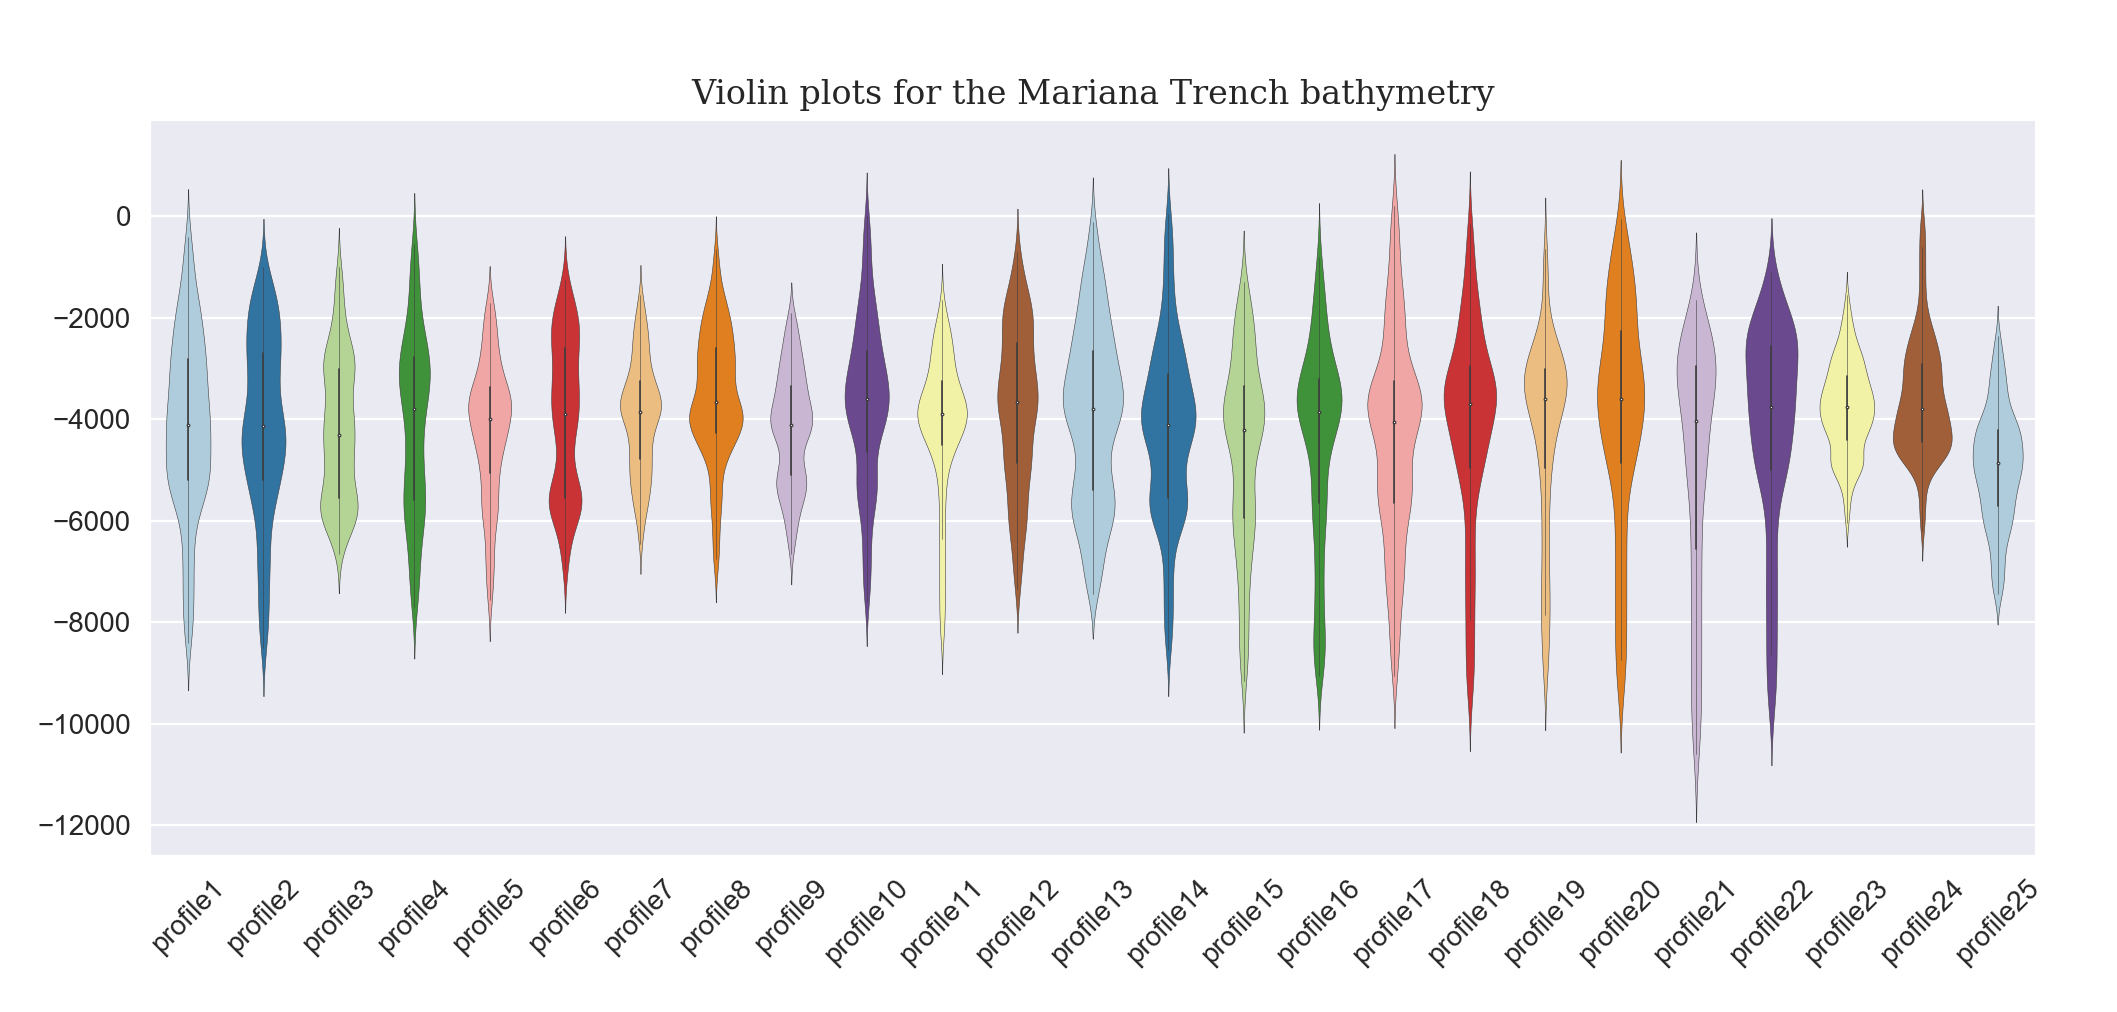
\includegraphics[width=13cm,clip]{Fig-COMU-3.jpg}
	\caption{Violin plots showing hydrographic depth ranges across the Mariana Trench. Plotting by Python code \ref{P:01}}\label{fig:COMU-3}
\end{figure}

Additionally, inside the violin shown the quartile and whiskers from the boxplot. As violin plot uses the \ac{KDE}, the wider portion of the violin plot shows, the higher density of the bathymetric observations. Vice versa, and narrow regions indicate very deep or very shallow values with lower density, rare across the bathymetric profile. The presented plot shows the distribution of the bathymetric values, i.e. depths along the bathymetric profiles. \\
The inter quartile ranges in the boxplot and higher density portion in KDE are placed in the same region of their categories within the violin plot. There is a notable decrease of depth in profiles 23, 24, 25 (Figure 3), crossing Caroline tectonic plate may be caused by the changes in the geologic properties of the tectonic plates. Profiles from Nr. 21 to 24 show the deepest depth data range with Nr 21 and 22 the most notable ones. Because the tectonic attribute values differ significantly, the comparative analysis of how the data vary across four distinctive tectonic plates was undertaken. 

\subsubsection{Hierarchically-clustered heatmap, clustermaps}\label{ssec:Py03}
The cluster map was plotted by Seaborn function seaborn.clustermap() to group bathymetric values within the 25 profiles by ranges. Ist structured representation arranges depth values by their semantic similarity using clustering method by ignoring outliers in colormap limits. While plotting clustermap Python assigns each of the 518 samples to a specific cluster of depths, divided into 6 groups with maximal cluster of depths over 7.500 meters. Cluster centers serves as a local target points with largest node resting at the center and attracting other values of bathymetric depths data that belong to this cluster. The clustermap (Fig. \ref{fig:MedFAR-6}) highlights groups of similar bathymetric depths with colors assigned as increasing darkness to the deepest values. The clustermap plotting was done using Python Seaborn library by Python code \ref{P:02}. 

\subsubsection{Histograms plotted by Python}\label{ssec:Py05}
Because Mariana Trench crosses 4 tectonic plates – Mariana, Pacific, Philippine and Caroline, the data set contained environmental variables separately for these plates that should be analyzed. This required merging the columns into one category: ‘tectonic plates’. Tsherefore, the columns with the plate names were melted into one class. Now the analysis of the data by plates became possible. The data were read in and processed as such by Python code \ref{P:04}. The histograms show the underlying frequency distribution of a submarine topography of the Mariana Trench (Figure \ref{fig:COMU-7}). Hence, it allows the inspection of the data for the type of distribution, that in this case is normal distribution, as well as outliers, skewness. The data are distributed and colored by tectonic plates: Mariana, Caroline, Pacific and Philippine Plates.

\begin{figure}[H]
	\centering
		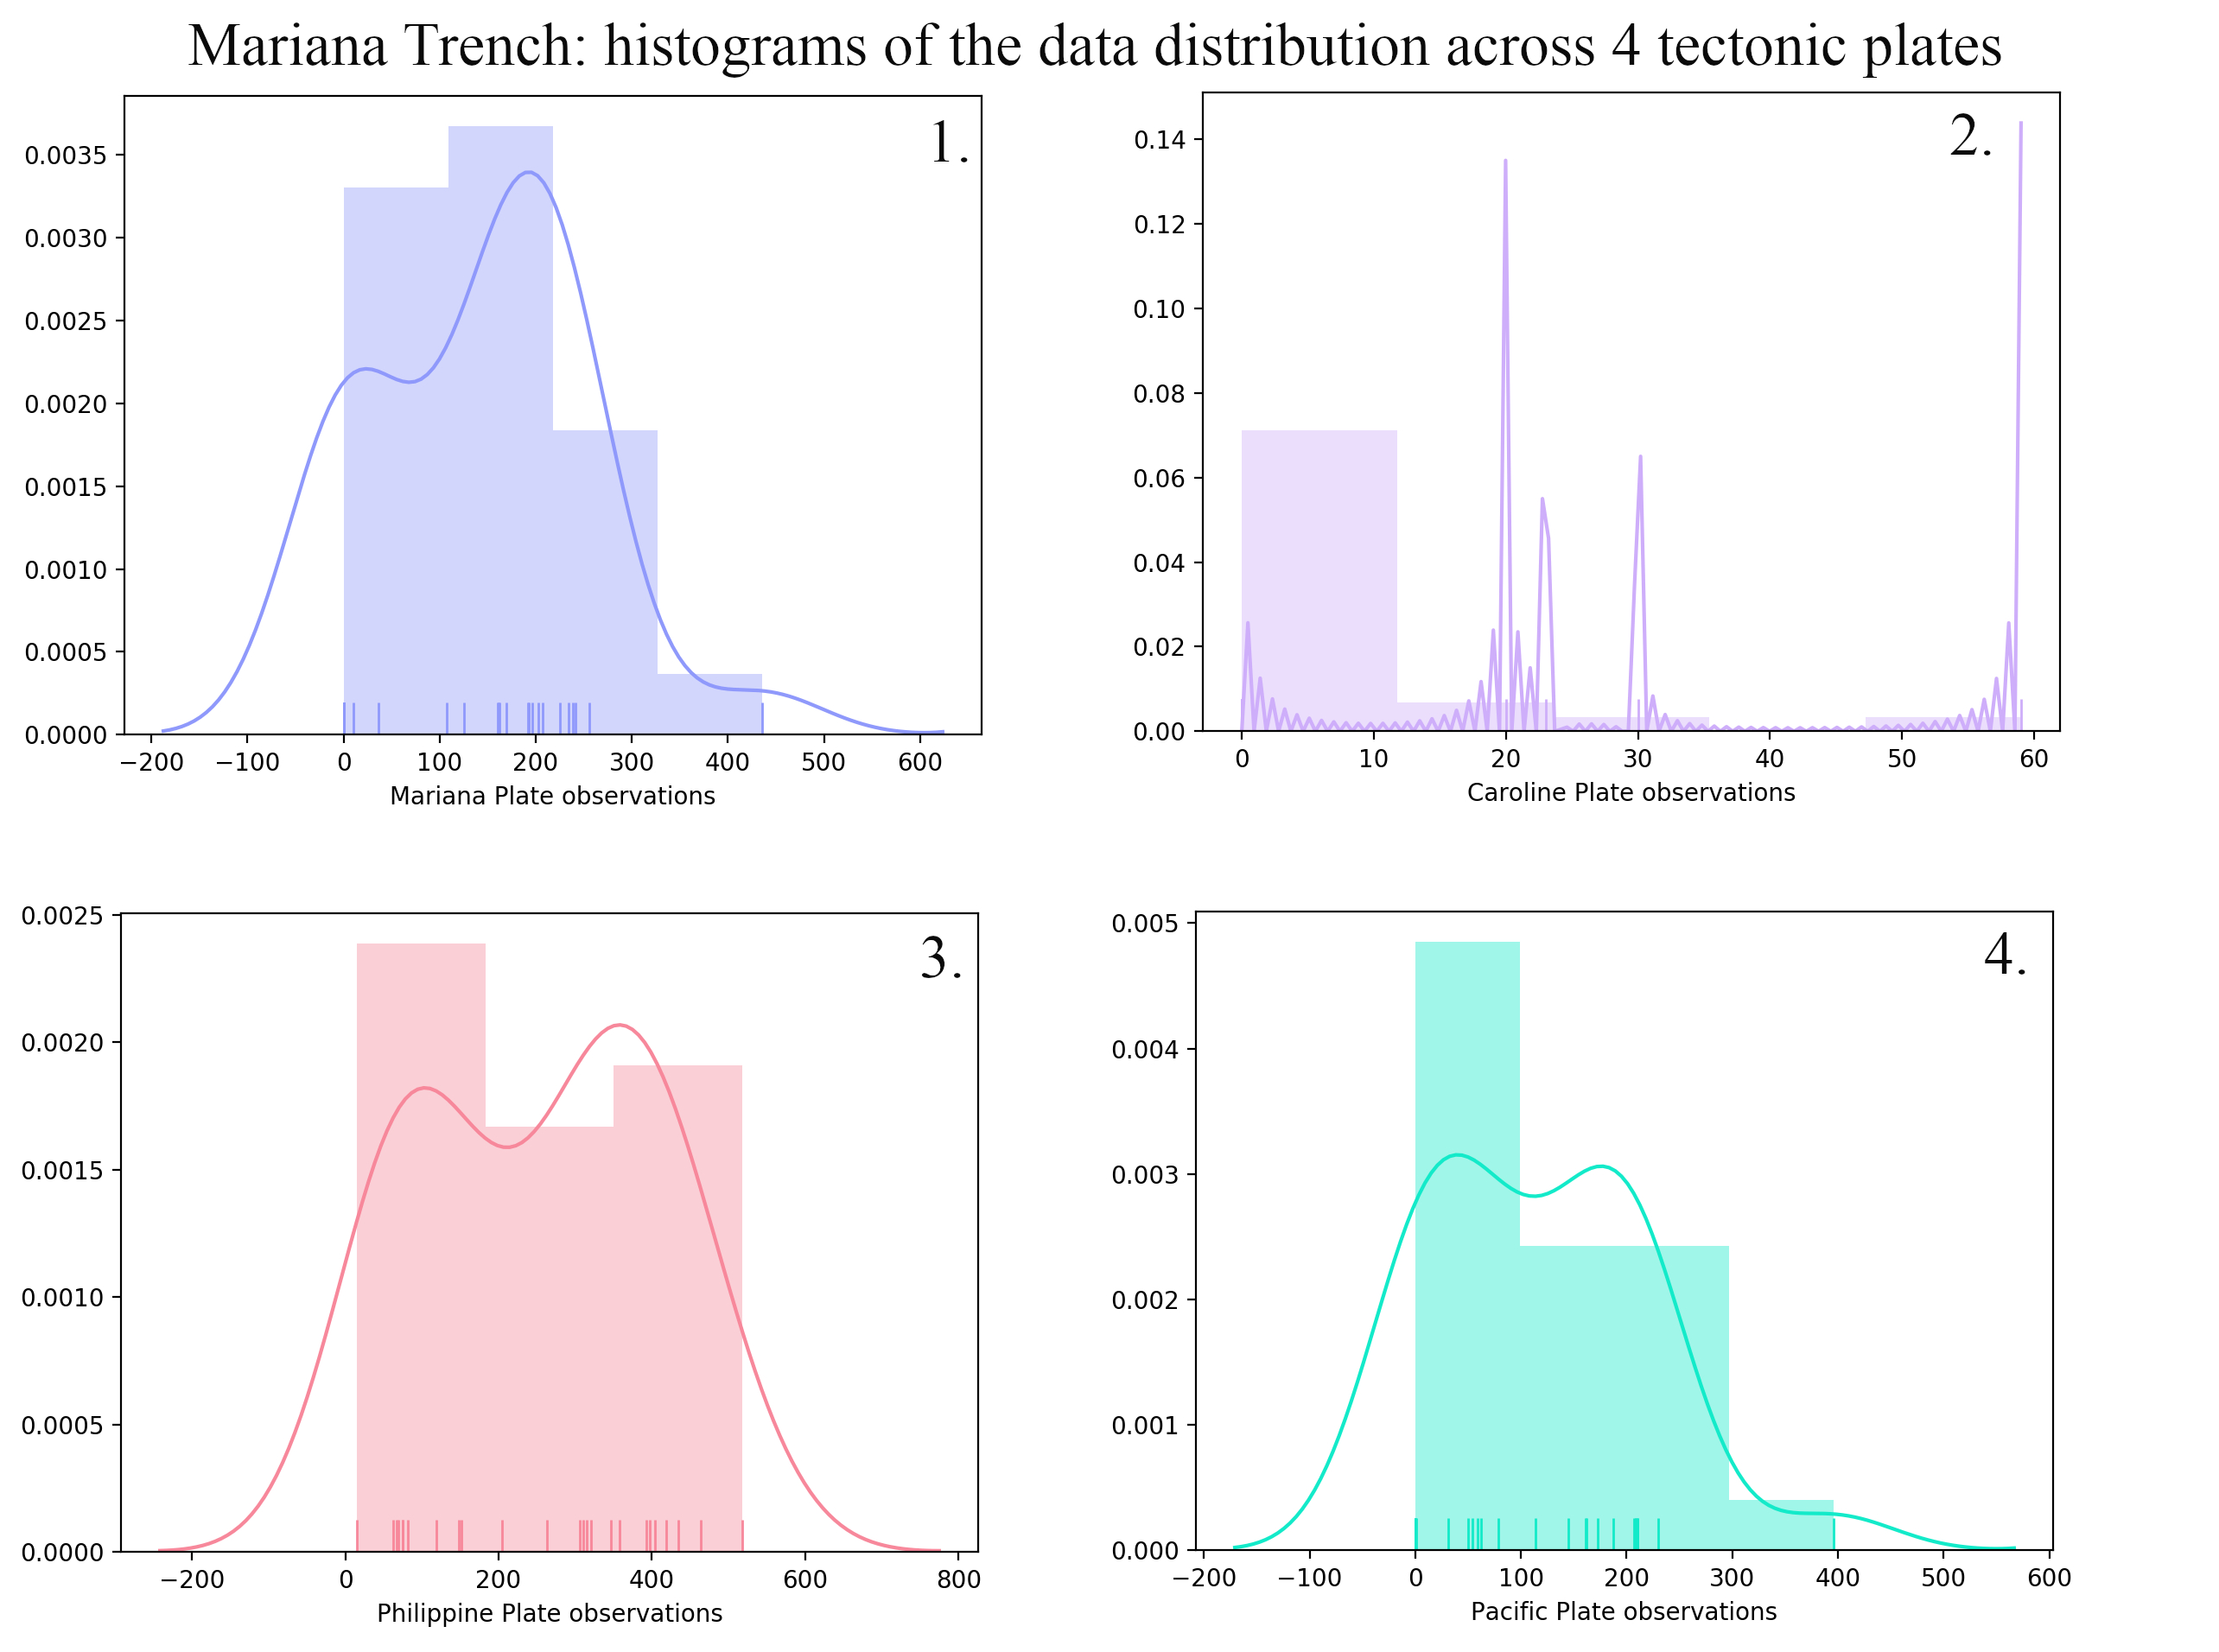
\includegraphics[width=13cm,clip]{Fig-COMU-7.jpg}
	\caption{Histograms of the data distribution across four tectonic plates.}\label{fig:COMU-7}
\end{figure}

\subsubsection{Strip plots by Python}\label{sssec:Py06}
The next step included visualizing strip plot showing the relationship between the sediment thickness and slope angles as compared by four tectonic plates crossing Mariana Trench using Python code \ref{P:05}. The particularity of the scatter strip plots (stripplot()) lies in its nature: this is a categorical types of plot showing variable dependance (maximal depths values by each profile) upon another variable, i.e. tectonic plates. It represents the depth values by 25 profiles sorted along each of the tectonic plates crossing the trench. In the above plot, one can see the difference on data distribution: the Caroline Plates has just only several points, since it crosses the trench in the south-western small part of the trench. Pacific and Mariana plates are relatively comparable, while Philippine Plate covers the majority of the data. As can be seen on Figure \ref{fig:COMU-7}, the majority of the observation points are located in the Pacific and Philippine plate, following my Marian plate, while Caroline plate only covers a few points. Sedimentation processes differ significantly by four tectonic plates (Mariana, Pacific, Philippine and Caroline), due to the overall complexity of the sediment environmental processes and trigger factors and mechanisms. 

\subsubsection{Euler-Venn diagrams by Python for visualizing logical relations}
	The Euler-Venn diagram shows four cases where overlapping in values or concepts can be visualized. The Figure \ref{fig:GP-9} (A) shows the cumulative total sediment thickness by tectonic plates. Figure \ref{fig:GP-9} (B) shows detected igneous volcanic spots. Figure \ref{fig:GP-9} (C) shows slope degree and Figure \ref{fig:GP-9} (D) shows methodological overlay showing the approaches of this work: GIS data mapping and digitizing, geological analysis and Python and R programming languages.
	
\begin{figure}[H]
	\centering
		\includegraphics[width=13cm,clip]{Fig-GP-9.jpg}
	\caption{Modelling intersection and correlation by various factors in the project Mariana Trench by Euler-Venn diagrams. A): Bathymetric observations by plates, cumulative computing; B): Sediment thickness, slope degree and closeness of the volcanic spots; C): Subdivision of the slope steepness by classes; D): Methodological approaches.}\label{fig:GP-9}
\end{figure}
The Euler-Venn diagram was done using Python programming code \ref{P:26}.

\subsection{Python library \emph{Seaborn}}\label{ssec:PySea}
This part of the work aims to refine the understanding of the poorly explained submarine geomorphic structure of the Mariana Trench by Seaborn application. A hadal trench located eastwards from the Philippine Sea, Mariana Trench has complex geomorphic structure and unevenness in profiles stretching south-westwards where its geomorphological structure is modified. The geomorphology is subjected to various phenomena that affect its shape. These include  bathymetry (depths), tectonics plates, geology (sedimentation) and geometry (slope steepness). A \ac{QGIS} based large dataset consisted of 12.950 observations and 25 profiles digitized across the trench with a 100-km distance in-between. In order to model such a large set of marine geological data, an object-oriented high-level programming language Python was selected as a refined tool due to its powerful functionality and effective coding solutions. A Seaborn library of Python was selected for geodata analytics and scientific plotting for data analysis. The data were read-in as a table in a .csv format and processed by statistical algorithms in Python libraries: Pandas for reading and processing tables, \ac{NumPy} for array analysis, Matplotlib for large dataset modelling, analysis and visualization. A statistical modelling aimed at the analysis of the relationships between the attribute factors using following methods: multiple facet grids, area charts for big data frames, regression analysis, letter-value plots for data distribution, hexagonal and Kernel density estimation, Pearson correlogram and clustermap. The scatterplot matrix was visualized by R language. The work includes Python codes for repeatability. The results of the data analysis show distinct unevenness of the geomorphic structure of the Mariana Trench.

\subsubsection{Regression Analysis}\label{ssec:PySea01}

\begin{figure}[H]
	\centering
		\includegraphics[width=13cm,clip]{Fig-MedFAR-3.jpg}
	\caption{Area chart and facet grid of the 25 cross-section bathymetric profiles of the Mariana Trench. Plotting visualization: Seaborn library, Python.}\label{fig:MedFAR-3}
\end{figure}

Initially, the 25 profiles were visualized by area chart and facet grid (Figure \ref{fig:MedFAR-3}). This gives an overview of the geometry (shape and steepness) and bathymetry (depths) of the profiles. Second, the regression analysis for the 25 profiles (Figure \ref{fig:MedFAR-4}) has been done using lmplot() function which is a figure-level function that combines regplot() and FacetGrid() functions of the Matplotlib, Python. The regression analysis was done using Python code \ref{P:07}.
	
\begin{figure}[H]
	\centering
		\includegraphics[width=13cm,clip]{Fig-MedFAR-4.jpg}
	\caption{Regression analysis: facet grid of the 25 cross-section bathymetric profiles of the Mariana Trench. Plotting visualization: Seaborn library, Python.}\label{fig:MedFAR-4}
\end{figure}
	
\subsubsection{Letter-value plots}\label{ssec:PySea02}
The features shown on the letter-value plot (Fig. 5) are distribution of the bathymetric data observations across 25 profiles. The statistical approach is derived from the Tukey's original boxplot principle \cite{Hofmannetal2011}. The letter-values plot shows a large number of quantiles in the bathymetric observation set, defined as “letter values”. The layout of this plot is similar to a box plot, however it is modified and improved. Besides plotting a nonparametric representation of a depths distribution across bathymetric profiles, where the data distribution corresponds to the observations, it plots more quantiles. 
	
\begin{figure}[H]
	\centering
		\includegraphics[width=13cm,clip]{Fig-MedFAR-5.jpg}
	\caption{Letter-value plot for data distribution, Mariana Trench bathymetric profiles. Plotting: Seaborn library, Python.}\label{fig:MedFAR-5}
\end{figure}

Therefore, the letter-values plot gives more deep inside into the shape of the bathymetric data distribution. Hence, it can be seen clearly that the maximal depths of the Mariana Trench are located in the south-western part of its crescent. Comparing to the box plot, the letter-value plot provides more detailed information in the ‘tails’ using letter values. Again, comparing to the box plots,  the letter-value plots on the bivariate big real data sets demonstrate to be more useful due to the more detailed approach on data analysis. The letter-value plots were done using Python code \ref{P:08}.
		
\subsubsection{Cluster heatmap and hexagonal data distribution and Kernel Density estimation}\label{ssec:PySea03}
Hexagonal mapping is another useful approach for analysis of the big data sets when there are many observation points that may overlap. In this case, the data set comprised 25 profiles with 519 observation points in each, which in total gives 12.950 points. In this case, hexagonal binning that plots density, rather than points shows the concentration of data values in the specific profiles (Fig. \ref{fig:MedFAR-6}, right). Depth points are binned into gridded hexagons and distribution (the number of depths ranges per hexagon). As a result, it is displayed (Fig. \ref{fig:MedFAR-6}, right) using the density of color within the hexagons. The kernel density estimation is a non-parametric approach that visualized the probability of the density of a depth variables by profiles (Fig. \ref{fig:MedFAR-6}, left). The joint Hexagonal and \ac{KDE} plots are drawn using Python code \ref{P:09}.
	
\begin{figure}[H]
	\centering
		\includegraphics[width=10cm,clip]{Fig-MedFAR-6.jpg}
	\caption{Heatmap for the data distribution: bathymetric profiles. Plotting: Python.}\label{fig:MedFAR-6}
\end{figure}

Another method used in this data analysis was a cluster map, that is a matrix plot dataset represented as a hierarchically-clustered ‘heat’ map. The core technique of the clustermap implies the graphical representation of the bathymetric data ranging from 0 to -10.000 meters, where the individual observation values are located in cells contained in a matrix and represented as colors (Fig. \ref{fig:MedFAR-7}). 

\begin{figure}[H]
	\centering
		\includegraphics[width=13cm,clip]{Fig-MedFAR-7.jpg}
	\caption{Hexagonal and \ac{KDE} plots: profiles of the Mariana Trench. Plotting: Python code \ref{P:09}}\label{fig:MedFAR-7}
\end{figure}

The color palette was selected as ‘reversed’, i.e. the most deep values are visualized as light purple values, and vice versa. The x axis shows the bathymetric profiles, the y axis shows the observation points in each profile. The color shows the depth recorded values. The left y axis shows the sub-division of the observations into hierarchical dendrograms starting from the two groups and soon, grouped based on the similarity of the depths. The records of geologic data (sediment thickness), submarine topography (slope angle degree and steepness by profiles) and bathymetry (absolute depth values: maximal and mean) on the map was also analyzed with respect to relationship in the dependence of the parameters. 
	
\subsubsection{Correlograms by Python}\label{ssec:PySea04}
Correlograms and covariance matrices give the background for all standard multivariate techniques, allowing to check for the randomness of data, as well as analyzing the data structure \cite{Friendly2002}. Current research tested three correlation methods (Pearson, Kendall and Spearman) to visualize the relationship between the environmental variances and representing a matrix of correlations schematically in forms numbers placed within the shaded squares (two of the three methods are shown on Fig. \ref{fig:COMU-9}). The numbers give the degree of the correlation, ranging from -1.0 to 1.0. In the shaded rows, each cell is given the assigned color, explained in the legend, subdivided into four classes ranging from two to four depending on the sign of the correlation. The intensity of color is scaled in proportion to the magnitude of the correlation. Several variations have interpreted the criterion of similarity of the properties and inter-relationships. A represented clustering of the matrix (a.k.a. heat map), made using Python code \ref{P:10}, shows the variables with the displayed correlations. The plotting of the correlation matrix induces a partial-ordering on the environmental variables as contiguous clusters.

\begin{figure}[H]
	\centering
		\subfloat {\includegraphics[width=7cm]{Fig-MedFAR-8.jpg}}
			\hspace{3mm}
		\subfloat {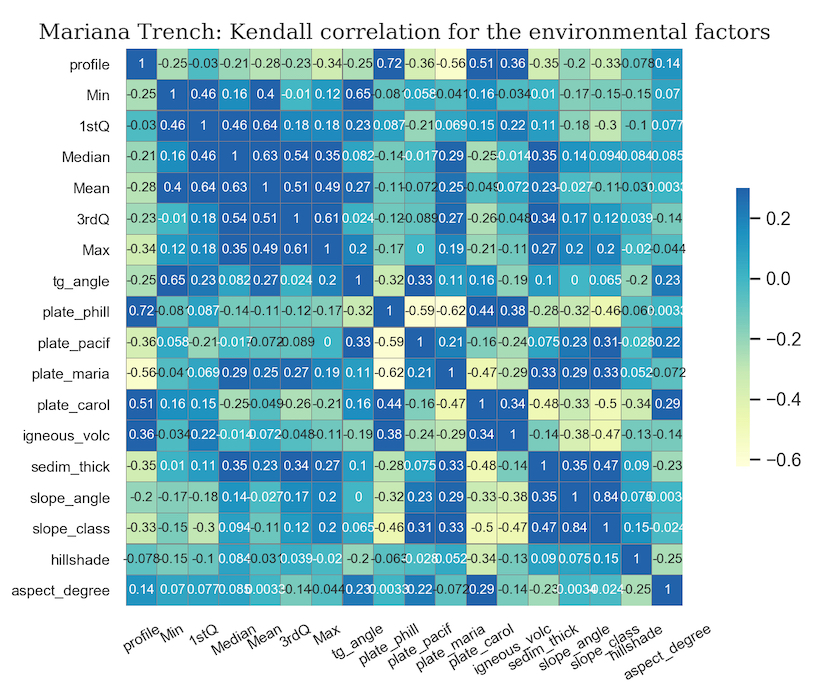
\includegraphics[width=7cm]{Fig-COMU-9.jpg}}
			\hspace{3mm}
	\caption{Correlation matrices for the environmental variables of the Mariana Trench: Pearson (left), Kendall (right)}\label{fig:COMU-9}
\end{figure}

The associated names of the environmental variables (e.g. slope angles, sediment thickness, maximal, minimal and mean depth values, etc) shown on the correlogram (Fig. \ref{fig:COMU-9}) were annotated on the axes, because the matrices were done using \ac{NumPy} and Pandas objects read in as tables and imported by the Seaborn library. The data were processed by Python code \ref{P:06}. The correlograms show the correlation between the factors affecting the Mariana Trench based on the relationships of the values. The effectiveness of the correlograms lies in its properties:  the diagonal shows the distribution of each of the environmental variables by a representative square plot which helps to analyze the relationship between the pairs of numerical variables within a matrix. The correlation between each pair of variable is visualize through a numerical symbols and highlighted by colors. The use of both Pearson and Kendall correlation techniques (Fig. \ref{fig:COMU-9}) is widely used for exploratory analysis to observe a matrix.

\subsection{Python library Matplotlib}\label{sec:PyMpl}
	
Understanding patterns of the correlation between the geomorphology and geology of the seafloor of the hadal trenches is important for the proper ocean modelling. Mariana Trench is the deepest hadal trench on the planet. Although the geodetic location, bathymetry and geologic structure of the tectonic plates are known to be associated with its geomorphic shape and geochemical content of the sediments, they have not been widely evaluated as large data sets by means of Python. An object-oriented high-level programming language, Python was selected for the marina geological data analysis and scientific plotting due to its powerful functionality and effective coding solutions used in methodology. Specifically, the statistical analysis includes the following steps: 

\begin{enumerate}
	\item Data distribution by the box plots; 
	\item Data sorting and grouping by stem plots; 
	\item Hierarchical clustering by dendrograms; 
	\item Clustermaps with grouped marginal dendrograms; 
	\item Correlation analysis by 3D comparative plots referred to 4 tectonic plates; 
	\item \ac{PCA}; 
	\item \ac{ANOVA}. 
\end{enumerate}

The statistical analysis of the 12,950 observation points constituting a data set showed correlation between the sediment thickness, slope steepness, depths and location of the bathymetric profiles crossing adjacent tectonic plates: Philippine, Pacific, Caroline and Mariana. \\
The data analysis in geosciences supported by Python programming language is an important novel method aimed to increase the precision of the computations and operating with big data, common in oceanography. However, performing data analysis while analyzing marine geological data sets is mounting a challenge. The existing solutions of the analysis of the oceanographic data mostly apply tradition methods of the \ac{GIS} using \ac{RS} observations data. This paper illustrated a Python based data analysis scheme based on the algorithms embedded by the Matplotlib library and its dependencies: \ac{NumPy}, \ac{SciPy} and Pandas \cite{Jonesetal2014}. The results show the effectiveness of Python programming in ocean modelling.
	
\subsubsection{Data distribution}\label{ssec:PyMpl02}
The box plots were plotted to demonstrate the data distribution across the 25 profiles with vertical lines extending from the boxes (so called whiskers) indicating variability of the depths outside the upper and lower quartiles. The plot was made via the following Python code \ref{P:11} and supported by the existing methods of the statistical analysis \cite{Friggeetal1989}; \cite{BatesWatts1988}; \cite{McGilletal1978}.

\begin{figure}[H]
	\centering
		\includegraphics[width=14cm,clip]{Fig-EgeJFAS-3.jpg}
	\caption{Box-and-whisker plot for the bathymetric depths distribution by 25 profiles}\label{fig:EgeJFAS-3}
\end{figure}

	Together with depth, the geomorphic shape of the Mariana Trench plays a crucial role in determining patterns of the sediment thickness in the proposed model. The depth ranges increased along the axis of the Mariana Trench, from north to the south of the trench, with a relatively constant slope gradient, until reaching depths overstepping 11,000 m (profiles 20 and 21 as shown on the Figure \ref{fig:EgeJFAS-3}). In the south-western part of the trench axis the modeled correlation between the factors was relatively high and yet decreased towards the south-western part of the profile. 
	
\subsubsection{Data sorting and grouping}\label{ssec:PyMpl03}
	
	A geomorphological analysis (Figure \ref{fig:EgeJFAS-4}) is technically based on the Python code \ref{P:12}. The geomorphological analysis uses only the calculated values of the slope steepness degree by profiles in the series of 25 cross-section bathymetric profiles (assuming constant values of the slope aspect), using bathymetric values and observation points as a reference. 

\begin{figure}[H]
	\centering
		\includegraphics[width=14cm,clip]{Fig-EgeJFAS-4.jpg}
	\caption{Stem plot of the geomorphic analysis of the slope steepness by 25 profiles.}\label{fig:EgeJFAS-4}
\end{figure}

This analysis shows that the (profiles Nr. 6, 9, 3, 7, 23 and 24) have the similar steepness and can be grouped as the lest steep, as demonstrated by the reverse values of the tangent angles. Conversely, the profiles Nr. 20, 21, 22, and 18 have the deepest values that can be explained by the changes in the geometry of the trench crossing different tectonic plates.  

\subsubsection{Data clustering: Hierarchical dendrogram and Clustermap}\label{ssec:PyMpl04}
	
	The general concept of the statistical approaches, algorithms and methods were derived from \cite{MarquesdeSa2007}. The \ac{HCA} as shown on Figure \ref{fig:EgeJFAS-5}, was done using \ac{SciPy} embedded algorithm of clustering. It demonstrates an approach of a method of cluster analysis used to build a hierarchy of bathymetric clusters based on the segmentation of the topographic features among 25 cross-section profiles. The dendrogram (Figure \ref{fig:EgeJFAS-5}) illustrates subdivision of the bathymetric values within each cluster composed by U-shaped link between a main cluster and its branches representing bathymetric grouping. The dendrogram showing the hierarchical dendrograms clusters was plotted using the Python code \ref{P:13} in five steps. 
	
\begin{figure}[H]
	\centering
		\includegraphics[width=12cm,clip]{Fig-EgeJFAS-5.jpg}
	\caption{Hierarchical cluster dendrogram of the geomorphic similarity among 25 bathymetric profiles of the Mariana Trench.}\label{fig:EgeJFAS-5}
\end{figure}

The two first forks of the of the U-link indicate which clusters were merged, while the length of each two corresponding branches visualize the distance between the ‘children’. Marginal dendrograms are represented on the Clustermap that shows another approach of data grouping in statistical analysis where the main area of the plot show the ranging data and the marginal dendrograms – the clusters of the similarity groups. 

\subsubsection{Data correlation}\label{ssec:PyMpl05}
	
The analysis data by correlation was performed using 3D scatterplot made by means of the ax.scatter() function of the Matplotlib library using Python code \ref{P:14} in 3 steps. 

\begin{figure}[H]
	\centering
		\includegraphics[width=13cm,clip]{Fig-EgeJFAS-7.jpg}
	\caption{3D Scatterplot of the interrelationships between the environmental factors.
}\label{fig:EgeJFAS-7}
\end{figure}

The 3D scatterplot matrices (Figure \ref{fig:EgeJFAS-7}) show variability of the geological, geometric and bathymetric factors (that is, sediment thickness, steepness of slope degrees and depth values) that is similar to the model by four tectonic plates: Pacific, Mariana, Caroline and Philippine. The sediment thickness is broadly correlated with the slope steepness degree, showing consistent geographic patterns by two pairs of plates: firstly, Mariana and Pacific, and secondly,  Caroline and Philippine (Figure \ref{fig:EgeJFAS-7}). 

\subsubsection{Principal Component Analysis (PCA)}\label{ssec:PyMpl06}
The \ac{PCA} was made using \ac{PCA} function from Sci-Kit Learn library of Python (from sklearn.decomposition import \ac{PCA}). Using orthogonal transformation procedure embedded in \ac{PCA} to convert a set of observations on sediment thickness and variables and possibly correlated variables into a set of values of linearly uncorrelated variables \cite{AbdiWilliams2010}. Using \ac{PCA} is an especially useful technique in case of marine geological large datasets and other implications of the big data in the geosciences, where there are many variables for each sample for exploratory data analysis \cite{Journel2000}. The \ac{PCA} enable to better visualize the variation presented in a dataset with many variables, that is sediment thickness, steepness of the slope angle and bathymetric depth ranges.

\begin{figure}[H]
	\centering
		\includegraphics[width=10cm,clip]{Fig-EgeJFAS-8.jpg}
	\caption{\ac{PCA} of the sediment thickness by 25 bathymetric profiles, Mariana Trench. 3D view.}\label{fig:EgeJFAS-8}
\end{figure}

The \ac{PCA} on the bathymetric spatial series was performed in order to assess the overall spatial geomorphic variability of the cross-section profiles and their similarities (Figure \ref{fig:EgeJFAS-8}). For this calculation the sediment thickness as a categorical value of the studied area was used. 

\subsubsection{\ac{ANOVA}}\label{ssec:PyMpl07}
The purpose of the \ac{ANOVA} in this research was to test for significant differences between means of the marine environmental variables, that is geological, tectonic and geodetic factors. Test differences in means for groups of mentioned above variables for the statistical significance was done using existing algorithms \cite{Gelman2005}; \cite{Montgomery2001}; \cite{Bailey2008}. The \ac{ANOVA} method is accomplished by analyzing the variance, that is, by partitioning the total variance into the component that is due to true random error (i.e., within-group SS) and the components that are due to differences between the means. It was performed using \ac{StatsModels} library of Python and Pandas for table data processing using Python code (5). Computed F values (0.270259 and 0.459078) and statistical significance obtained from testing with \ac{ANOVA} shows the effect of depth and model scenario on the sediment thickness estimated through the \ac{StatsModels} library of Python (statsmodels.stats.anova anova\_lm). The correlation cluster dendrogram between a spacial series of the cross section profiles shows a grouping between the profiles based on their geomorphic similarities. The analysis of variance was done using \ac{StatsModels} library of Python and embedded function \ac{ANOVA} by the Python code \ref{P:15}. 

\begin{figure}[H]
	\centering
		\includegraphics[width=13cm,clip]{Fig-EgeJFAS-10.jpg}
	\caption{One-way \ac{ANOVA} box plots showing a potential relationship between selected environmental, bathymetric and geomorphological variables by analysis of similarities.}\label{fig:EgeJFAS-10}
\end{figure}

The deep-sea sediments has consistent correlation with the slope class of the profile steepness as shown on Figure \ref{fig:EgeJFAS-10} (c). Lower effect has the location of the igneous volcanic areas nearby the trench on the geometry of the profiles, as referred by the angle degree (Figure \ref{fig:EgeJFAS-10}, d). While the shape of the trench is less steep and the absolute depths are lower in the upper part of the trench, that is, north-east while crossing the Pacific and Mariana tectonic plates, the bathymetry patters is substantially deeper in the south-eastern part of the Mariana Trench where it is crossing Caroline and Philippine Sea Plates. These findings are also supporting the results of \cite{ZhouLin2018} who studied variations in the deformation of the subducting plate along the Mariana Trench by analyzing its flexural bending and normal fault features. They reported that most normal faults initiated outwards and grew toward the trench axis, and the trench relief and maximum fault throws are significantly greater in the south (5 km and 320 m) comparing to the northern and central areas (2 km and 200 m).

\subsection[Data Processing by Python Libraries NumPy, SciPy \& Pandas]{Data Processing by Python Libraries NumPy, SciPy and Pandas}\label{sec:PyPan}
	
\subsubsection{Methodological flowchart network of the section}
The study area is located in west Pacific Ocean, Mariana Trench. The aim of the data analysis is to analyze the potential influence of how various geological and tectonic factors may affect the geomorphological shape of the Mariana Trench.  Statistical analysis of the data set in marine geology and oceanography requires an adequate strategy on big data processing. In this context, current research proposes a combination of the Python-based methodology that couples \ac{GIS} geospatial data analysis. The \ac{QGIS} part of the methodology produces an optimized representative sampling dataset consisting of 25 cross-section profiles having in total 12.590 bathymetric observation points. The sampling of the geospatial dataset are located across the Mariana Trench. The second part of the methodology consists in statistical data processing by means of high-level programming language Python. Current research uses libraries Pandas, \ac{NumPy} and \ac{SciPy}. The data processing also involves the subsampling of two auxiliary masked data frames from the initial large data set that only consists of the target variables: sediment thickness, slope angle degrees and bathymetric observation points across four tectonic plates: Pacific, Philippine, Mariana and Caroline. The methodological flowchart includes three main stages (Figure \ref{fig:AR-2}) visualized as the logical parts of this research: first, \ac{GIS} part using \ac{QGIS}, second, statistical analysis on Python language; third, spacial analysis of the data similarities on R language.\\
	First block consisted in processing oceanographic data using\ac{QGIS}software: data import, digitizing profiles, data export into .csv tables for further processing in Python and R. The cross-section profiles were digitized and the attribute tables were created (Figure \ref{fig:AR-1}). The tables contained numerical information on geology, tectonics, oceanography and bathymetry by observation points along each profile. In total there was 25 profiles, each containing 518 observation points. Hence, the total data intakes consisted in pool of 12.590 points. \\
	Second block contained in data interpretation and statistical analysis. The steps include following approaches of the statistical data analysis: 
	
\begin{enumerate}
	\item \ac{KDE} for analysis of the probability of data distribution; 
	\item stacked area chart for visualization of the data range across various segments of the trench;
	\item spacial series of radar charts; 
	\item stacked bar plots showing the data distribution by tectonic plates;
	\item stacked bar charts for correlation of sediment thickness by profiles, versus distance from the igneous volcanic areas;
	\item circular pie plots visualizing data distribution by 25 profiles;
	\item scatterplot matrices for correlation analysis between marine geologic variables. 
\end{enumerate}

	Third block presents the geospatial analysis of the data correlation. This implies correlation analysis of the scatterplot matrices by visualizing geological and tectonic interplay between the phenomenas. The scatterplot matrices for correlation analysis between marine geologic variables were performed using R language.\\
	The results presented distinct correlation between the geologic, tectonic and oceanographic variables. Six Python codes are provided in full for repeatability of this research. Nevertheless, the problem of the proper understanding of the hadal areas in the ocean lies in its unreachable location. As justly noted by \cite{Jamieson2018}, understanding marine ecosystems for proper management and use of marine resources has a certain paradox, since there is a need to evaluate and protect the marine life and ocean ecosystems. However, the current knowledge on ocean functioning is relatively scarce. At the same time, modeling ocean and marine environment is a critical for the sustainable development of ocean resource usage. Recent studies only stress the strong correlation of the research with increasing ocean depths. However, the majority of the recent methods of ocean observations have overlooked the Python programming approach for statistical analysis where the large data sets are being processed by e set of the embedded mathematical algorithms. Here, the paper presents improvements on the oceanographic data processing and interpretation methods by applying Python 3.2.7 languages and using its most essential libraries: \ac{NumPy}, \ac{SciPy}, Pandas and Matplotlib for data visualization and analysis.\\
	Various mathematical algorithms used in this work were applied from the statistical functionality provided by Python language \cite{Beazley2009}. The \ac{SciPy}, an extension of \ac{NumPy}, is another Python based package that was loaded for mathematical computations. The specific questions of usage SciPy were supported by large explanations of the \ac{SciPy} principles and its usage in the statistical analysis.
	
\begin{figure}[H]
	\centering
		\includegraphics[width=10cm,clip]{Fig-AR-2.jpg}
	\caption{Methodological network}\label{fig:AR-2}
\end{figure}

\subsubsection{\ac{NumPy} for processing arrays}
Using Python modules and libraries enables processing of the large oceanographic data more effective and significantly improves the computation algorithms. The general functioning of the Python followed the existing references and manuals, \cite{Oliphant2007}; \cite{Pedregosaetal2011}; \cite{PerezGranger2007}. Using libraries enable to create namespaces while working with modules. Python’s modules contain packed classes, objects, functions and constants used in the work. The installation of the libraries was done using pip upon the installing \ac{NumPy} and \ac{SciPy}, its dependancies: \\
\$ python3 -m pip install numpy
\$ python3 -m pip install scipy 
The sorting and selecting of read in data from the tables was performed using NumPy. NumPy creates a multidimensional array object from a given ‘table.csv’. Using Python’s syntax and semantics, it operates with matrices using logical, bit-wise, functional operations with elements, and performs a series of routines for fast operations on arrays \cite{NumPyCommunity2019}. Finally, \ac{NumPy} enables various object-oriented approach, mathematical and logical manipulations with table using ndarray. The scripts, modules and codes were written using reference semantics and built-in functions of \ac{NumPy} and Python. The saved script included the written codes that parse command lines and perform graphs plotting by executing functions and modules. The namespaces of NumPy were imported from numpy.core and numpy.lib by calling:\\
>>> import numpy as np
The depending libraries have been installed as well. These include Jinja2, \ac{NumPy}, Pillow, PyYAML, Six, Tornado. Manipulating with tabular data stored in csv files has been implemented in suitable Python library Pandas optimized for the high-level processing of tabular data. The Matplotlib library was installed as well and imported to customize plots. 

\subsubsection{Probability of the depths distribution by \ac{KDE} plots}

	In this part of the work, an implementation of the fundamental frequency estimation is presented. The algorithm of \ac{KDE} is based on a frequency-domain approach (Figure 3). It was applied to visualize probability of the depth ranges and bathymetric patters in various segments of the Mariana Trench. The method was implemented using Python code \ref{P:16}. Python libraries Pandas, Matplotlib, Seaborn and OS were used to process data by an embedded algorithms to obtain probability frequency. 

	\subsection{Visualizing bathymetric pattern by stacked area charts}
In marine geologic data sets, plotting stacked area charts is one of the key approaches to visualize the range of the bathymetric depths. In other words, we can answer the question of to what extent are the depths may reach in this or that particular segment of the trench? Apart from the visual clearance of the plot (Figure \ref{fig:AR-4}), showing the maximal abrupt depth by profiles 20 and 21 (that is, south-west of the Mariana Trench), there are other interesting particularities in this approach. 

\begin{figure}[H]
	\centering
		\includegraphics[width=12cm,clip]{Fig-AR-4.jpg}
	\caption{Mariana Trench: bathymetric patters visualized by stacked area charts.}\label{fig:AR-4}
\end{figure}

Thus, on can investigate different phenomena of the oceanographic data sets by adding color ranges for stepwise visualization of the plot, sub-divided by statistical steps: minimal depths, third quartiles, mean depths, median values of the depths, first quartile, and finally, the shallowest parts of the geomorphology, that is the minimal depths. In this way, one can understand the variability of the geomorphic patters by the segments that could reveal new insights into how the bathymetric data variability affects the complex geomorphology of the profile. The methodology was implemented using Python code \ref{P:17}. The following Python libraries were used to plot stacked area charts: Pandas, \ac{NumPy}, Matplotlib, Seaborn and OS. 

\subsubsection{Statistical distribution of the bathymetric values by radar charts}
Of particular interest is the case of radar charts. Recently, radar charts turned into a very interesting visualizing method in the data analysis. A radar chart is a graphical method of displaying multivariate data in the form of a two-dimensional circular chart of six quantitative variables represented on axes bathymetric depths and on the circular axes bathymetric values: maximal, \nth{3} quartile, median, mean \nth{3} quartile and minimal values. 
\begin{figure}[H]
	\centering
		\includegraphics[width=13cm,clip]{Fig-AR-5.jpg}
	\caption{Series of the radar charts showing variation on the bathymetry by selected profiles.}\label{fig:AR-5}
\end{figure}

The reason to choose the radar charts is that there are various statistical values that camn be visualized by profiles, which requires a certain visualization technique for the facetted multi-plots (Figure 5). The series of the radar charts were plotted by libraries Math, Pandas, NumPy, Matplotlib, Seaborn and OS. The algorithm for the radar charts was taken from the Matplotlib library and the Python code is provided below: \ref{P:18}. 

\subsubsection{Variation in the distribution of the bathymetric data by stacked bar plots}
	Figure 6 shows the variation in the distribution of the bathymetric data by stacked bar plots
The following Python libraries were used to plot stacked area charts: \ac{NumPy}, Pandas, Matplotlib and OS. The distribution of the bathymetric data by stacked bar plots was plotted using open source Python code: \ref{P:19}.  

\begin{figure}[H]
	\centering
		\includegraphics[width=12cm,clip]{Fig-AR-6.jpg}
	\caption{Stacked bar plots showing variation in the distribution of the bathymetric observations by the profiles, Mariana Trench.}\label{fig:AR-6}
\end{figure}

\subsubsection{Analyzing distribution of the sediment thickness by stacked bar charts}
	Analysis of the distribution of the sediment thickness is visualized by the stacked bar charts (Figure \ref{fig:AR-7}). The Python code \ref{P:20} in 7 steps provides an approach to visualize the sediment thickness by profiles and its correlation with closeness of the igneous volcanic areas as by distance. The code was written using calling following Python libraries: \ac{NumPy}, Matplotlib, Pandas and OS. 
	
\begin{figure}[H]
	\centering
		\includegraphics[width=13cm,clip]{Fig-AR-7.jpg}
	\caption{Stacked bar charts showing distribution of values of sediment thickness by profiles (left), versus distance from the igneous volcanic areas (right), Mariana Trench.}\label{fig:AR-7}
\end{figure}

\subsubsection{Circular visualization of the bathymetry versus tectonic plates by pie charts}
	Regarding the categorial distribution methods, a pie chart plotting is based on the analysis of the bathymetric distribution of the values by four tectonic plates (Figure \ref{fig:AR-8}). Circular visualization of the bathymetry showing the relationship between tectonic plates and distribution of bathymetric data by pie charts was performed by Python code \ref{P:21} in 3 steps. It used the following Python libraries: Pandas, NumPy, Matplotlib and OS.  

\begin{figure}[H]
	\centering
		\includegraphics[width=13cm,clip]{Fig-AR-8.jpg}
	\caption{Circular visualization of the data distribution: bathymetric observation points by tectonic plates. Visualization method: pie charts.}\label{fig:AR-8}
\end{figure}

\subsection{Python libraries Matplotlib, Seaborn and Bokeh: analysis of bathymetric data distribution}

The data distribution are presented on Figure 3. By profiles they ranged from -10.600m (maximal depth in this data set) to -3150m (the shallowest point in the data set). The maximum depths in the profiles were found in profiles Nr. 20, 21, 19, 14 (Figure 3, right, sorted bathymetry), and the minimal depths (i.e. the shallowest) consist the first group, that is profiles 24, 23, 22 and 10 (Figure 3, right, sorted bathymetry). The deepest part of the trench is located in the south-west and central segments where the trench crosses Philippine and Pacific Plates. The moderate depths correlate with Mariana Plate and the majority of the Philippine Plate. The depths ranges detected across the profiles of present study are also higher in southern part of the trench than in northern segment (Figure 3).

\begin{figure}[H]
	\centering
		\includegraphics[width=13cm,clip]{Fig-GP-3.jpg}
	\caption{Data distribution analysis: ranges of the maximal bathymetric depths by 25 cross-section profiles across the Mariana Trench}\label{fig:GP-3}
\end{figure}

 In general, the central part of the Mariana Trench has variations in depth but the general trend shows the increased depths towards the southern part were the depths are higher than in the northern segments. By comparing the profiles Nr. 3, 4, 9, 12 from the Pandas array (Figure \ref{fig:GP-3}, colored green) with profiles Nr. 18, 16, 15, 13 from the Pandas array (colored orange on Figure \ref{fig:GP-3}), it is clear that the depths increase reaching its maximal depths in the following group (Profiles Nr. 20, 21, 19, 14, group colored blue, Figure \ref{fig:GP-3}, right). 
Methodological goal os this research was to identify variations of the steepness in various segments of the trench. The slope steepness degrees and depths of the profiles were analyzed and determined based on the statistical analysis using libraries of Python: Matplotlib, Seaborn and Bokeh. The results revealed that the most steep part of the trench is located in its north-west, central and south-west segments (profiles Nr. 3, 7, 9, 23, 24) where trench crosses Philippine and Pacific tectonic plates. \\
This segment of the trench can be characterized by the largest local depths and sharp abrupt changes in the geomorphic shape. The highest depth gradient can be seen at the profile Nr. 21 is at the distance of 10.600 m from the seal level. The middle moderate slope degrees (Profiles Nr. 1, 11,  4, 5, 10) correlate with the areas where trench crosses Mariana tectonic plate. 
 
 \begin{figure}[H]
	\centering
		\includegraphics[width=13cm,clip]{Fig-GP-4.jpg}
	\caption{Visualization of the cross-section profiles, Mariana Trench}\label{fig:GP-4}
\end{figure}

Now we can have a more detailed look on the profiles’ shape and the outline (Figure \ref{fig:GP-4}). While Figure \ref{fig:GP-3} shows the maximal depths by profiles (i.e. each profile has only one dot point on the plot), the Figure \ref{fig:GP-4} illustrates the cross-section profiles. Among the various shapes of the profiles in present studies (Figure \ref{fig:GP-4}) the section of profiles 19, 20, 21 and 22 (Figure \ref{fig:GP-4}, E) had initially the most even shape of the geomorphology that started decreasing abruptly after the observation points 200. The unevenness of the profiles can be explained by the changes geologic conditions and transfer to the neighbor tectonic plate (i.e. from the Philippine Plate to the Pacific Plate, and Mariana Plate to the Philippine Plate, respectively). 

\begin{figure}[H]
	\centering
		\includegraphics[width=13cm,clip]{Fig-GP-5.jpg}
	\caption{Data distribution analysis: ranges of the maximal bathymetric depths by 25 cross-section profiles across the Mariana Trench}\label{fig:GP-5}
\end{figure}

The groups of profiles 23, 24 and 25, (Figure \ref{fig:GP-4}, F), have the similar geomorphic shapes: the first halve of the profiles is relatively even while the southern part is particular for the increased depths. This and analogous analyses can be drawn from the Figure \ref{fig:GP-4}. For better visualization, the profiles are colored individually with the shared X axes. The increase of depths by profiles can be influenced by multiple various factors including geographic location and location on subducting tectonic plates, geologic settings of the sediment accumulation as well as exposure to other oceanological and environmental factors. A jitter plot visualization of the overlapped observation points by profiles (Figure \ref{fig:GP-5}) shows the concentration of the most frequent, repeated depths by profiles is visualized. That is, comparing to the previous figures (Figure \ref{fig:GP-3} and Figure \ref{fig:GP-4}) where the focus is set up on the data range, the Figure \ref{fig:GP-5} stresses the analysis of frequency in the data range. The Figure \ref{fig:GP-5} is plotted using Bokeh library of Python.
The geomorphic segments of the Mariana Trench have a relatively balanced bathymetric elevations records ranging from -7.600 m (profile Nr. 11), -7.750 m (profile Nr. 4), -7.800 m (profile Nr. 5),  -7.750 m (profile Nr. 10), to -6.200 m (profile Nr. 1). The modelled depths are shown in on Figure \ref{fig:GP-5} (jitter plot showing depths ranges). The profiles with the least slope degree Nr. 21, 22, 18, 20 are mostly located in the southern segments where trench crosses Caroline Plate. Mostly, the depth values of deeper than -9600 m below the sea level prevails on the bathymetric model for the deepest depth range (Figure \ref{fig:GP-5}), representing the depths of the very steep slopes of the Mariana Trench.  
	
\subsection{Python Library StatsModels for linear regressions}
This research section aims is to apply linear regression statistical approaches for oceanological data interpretation. Specific aim is to investigate correlation between various factors, such as bathymetric depths, geomorphic shape, geographic location on four tectonic plates of the sampling points along the trench, and their influence on the geologic sediment thickness. Technically, the advantages of applying Python programming language for oceanographic data sets was tested. The methodological approaches include GIS data collecting, data analysis, statistical modelling, plotting and visualizing. Statistical methods include several algorithms that were tested: 
\begin{enumerate}
	\item weighted least square linear regression between geological variables;
	\item autocorrelation; 
	\item design matrix;
	\item \ac{OLS} regression;
	\item quantile regression.
\end{enumerate}
The spatial and statistical analysis of the correlation of these factors aimed at the understanding, which geological and geodetic factors affect the distribution of the steepness and shape of the trench. Following factors were analyzed: geology (sediment thickness), geographic location of the trench on four tectonics plates and bathymetric depths records along the profiles: max, mean, min values, as well as the statistical calculations of the \nth{1} and \nth{3} quantiles. The study revealed correlations between the sediment thickness and distinct variations of the trench geomorphology and sampling locations across various segments along the crescent of the trench. 
	
\subsubsection{Design matrix and model fit summary by the Ordinary Least Squares}
	The variables of geologic interest were stored in the table consisting of 18 rows where numeric information describes geology, bathymetry, geodesy and tectonics of the Mariana Trench. To fit most of the models covered by \ac{StatsModels} Python library, the design or regressor matrix was created using existing approaches \cite{Everitt2002}; \cite{BoxTiao1992}; \cite{MillmanAivazis2011}. The first is a matrix of endogenous variables of sediment thickness, which show the response or geological regressand on changed environmental conditions: geographic location, depth or tectonic plate. The design matrix ‘dmatrices’ shows the results of the first six lines representing values of explanatory variables in a set of geological attributes, Mariana Trench. The computing of the \ac{OLS} by StatsModels of Python was based on the formula (1):
Formula (1)
Where,      
n is the sample size;
x is a constant and a scalar regressor; 
y is a random regressor, sampled together with x;
h is the number of lags being tested;
Each row of the calculated \ac{OLS} coefficient estimates is an individual bathymetric profile with the successive columns corresponding to the geologic and oceanographic variables and their specific values across the profiles. 
	
\subsubsection{Quantile statistics (QQ)}
	The used algorithm is very straightforward with a selected function of qqplot() by StatsModels to perform this task. The \ac{QQ} regression is a common abbreviation for ‘quantile by quantile’ statistical plot. The plot shows (Fig. 2, \cite{Lemenkova201989}) one quantile against another across various geological parameters: Sediment thickness; Slope angle degrees; four tectonic plates; distribution of the samples of igneous volcanic areas. Technically, the plotting was performed using Python code \ref{P:22} for each corresponding plot. The \ac{QQ} statistics calculation has been based on the following formula (2) after \cite{LjungBox1978}:
Formula (2)
Where,      
n is the sample size;
$rho$ is the sample autocorrelation at lag k, and 
h is the number of lags being tested.\\
The comparison of all the six subplots enables to analyze the form of their shape against a straight line. The quantiles are bathymetric sample observations with geologic attribute values placed in the ascending order. The \ac{QQ} statistics is used over the pool of the sampling data to study their distribution. A \ac{QQ} statistic is a visual representation of the quantiles of a standard normal distribution of the geological data set across the Mariana Trench, showing their variation in space. \\
The quantile regression estimates conditional median and other quantiles of the response geological variables. Thus the upper two rows of the plot show (Fig. 4 in \cite{Lemenkova201989}) data distribution for sediment thickness (m) versus geologic parameters across tectonic plates, data distribution for the cumulative sediment thickness and slope angle degree by profiles. The quantile regressions were plotted (Fig. \ref{fig:ASE-4}) using Python code \ref{P:24} by \ac{StatsModel}. Essentially, quantile regression is another approach of the linear regression tested in the current research. The quantitative results of the quantile regression are shown on Tab. 3 in \cite{Lemenkova201989} which shows computations for the quantile regression for sediment thickness versus geologic parameters and tectonic plates. 
	
\subsubsection{Weighted Least Squares}
A \ac{WLS} for the geological variables analysis data distribution: by tectonic plates, sediment thickness and bathymetry, as well as slope angle degree. A \ac{WLS} is a statistical approach representing a special case of the generalized least squares. The approach of a weighted least squares is a standard approach in regression analysis to approximate the solution of overdetermined systems which is the case for the complex marine geological systems. The least squares algorithms has two sub-types: linear or ordinary least squares and nonlinear least squares. In the scope of this research, only the linear least squares were tested: ordinary least squares and weighted least square which is a generalization of the first one. In this case, the off-diagonal entries of the correlation matrix of the geological residuals are null the variances of the observations, yet unequal along the covariance matrix. The calculation is based on the principle of the Gauss-Newton algorithm that solves a non-linear least squares problem by modifying a Newton's method for finding a minimum of a function. The computation was based on the general approach of existing equation (after \cite{Bjoerck1996}):

Formula (3)
Where 
W is a diagonal when the observational errors are uncorrelated and the weight matrix;
J (t) is a transposed Jacobian matrix;
β are unbiased estimators as linear column vectors, the entries of the Jacobian matrix;
y is a vector of the response values.

The calculations of the \ac{WLS} for the data se shows computations of the \ac{WLS} modelling for the data distribution by plates, \cite{Lemenkova201989}, done according to the reported procedures \cite{SeaboldPerktold2010}; \cite{Strutz2016} by the Python code snippet \ref{P:23}.

\subsubsection{Isotonic regression}

The statistical numerical method of the isotonic regression was applied as a non-metric multidimensional scaling aimed at fitting a line to a sequence of the observations provided the line has variation in forms, that is non-decreasing and or non-increasing everywhere across the observations. Furthermore, the line lies most close to the observations pool. The concept of the isotonic regression has been introduced by \cite{Kruskal1964} and further developed by \cite{BestChakravarti1990}. The principle of the computation algorithm of the isotonic regression lies in the following formula of the problem of \ac{QP}: 

(FORMULA-1)
 Where,      
x(i) and x(j) are constraints;
E are the edges or the is the set of pairs (i, j) for each constraint;
w is a weights vector;
n is a number of observations.
The isotonic estimator, g minimizes the weighted least squares-like condition:

(FORMULA-2)
 Where, 
A is the set of all piecewise linear, non-decreasing continuous functions; 
f is a known function. 
Further references on isotonic regression and its applications are given by \ref{Wuetal2017}. The presented plot of the isotonic regression (Figure \ref{fig:GP-7}) shows a non-decreasing approximation of a function while minimizing the mean squared error on the training bathymetric data set of the 25 profiles. 

\begin{figure}[H]
	\centering
		\includegraphics[width=13cm,clip]{Fig-GP-7.jpg}
	\caption{Isotonic regression for the selected variables: geological data on sediment thickness layer (A) and maximal depths recorded by 25 profiles (B).}\label{fig:GP-7}
\end{figure}

The benefit of this kind of a model is consists in the flexibility of the model, that is, the function does not assume any form for the target function such as linearity. Thus, the real data o the observed values by 25 profiles can be compared with the isotonic curves (Figure \ref{fig:GP-7}). Further references are given by \cite{Leeuwetal2009}.
	
\subsubsection{Dynamic regression model: SARIMA}
	The methodology of the dynamic regression model is based on the StatsModels embedded algorithm \cite{SeaboldPerktold2010}. The abbreviation \ac{SARIMA} stands for the model, initially developed by \cite{AnsleyKohn1985}. The concept of the application of the \ac{SARIMA} time series estimation and post estimation lies in the following. The changes in the variables that are taken as time lags in classic dynamic regression models are applied towards bathymetric profiles from 1 to 25. In this way, unlike in time series case when the ARIMA fits the univariate models with time-dependent disturbances, this case applies space-dependent disturbances, crossing the sampling (X axe), \cite{Lemenkova201989}. \\
	Because the model includes both dependent and independent variables, the selected type of \ac{SARIMA} was \ac{SARIMA}X (see the Python code snippet {P:25}). The first group consists in changing variables that is geologic settings and bathymetry (depths). The second group (independent variables) is presented by the profiles lags that cross the Mariana Trench with the distance between each of 100 km and the length of 1000 km. This cross-section profiles are taken as independent variables. Therefore, the dependent variables differ spatially in different segments of the trench. Python code for used SARIMAX algorithm and Statespace Model Results, \cite{Lemenkova201989}. Tested case is a Mariana Trench tectonics: sediment thickness across Philippine Plate. The model fits univariate model of the geomorphic structure of the trench by independent values of the distribution of the bathymetric observation by profiles with dependent disturbances of depths. Fitting the model was done using the Python snippet {P:25}.\\
	The conducted statistical data modelling and several types of the regression analysis were aimed to compare the variance in the geological data sets of the Mariana Trench explained by the complex interplay of the geomorphic, geological and oceanological attributes of the data and the bathymetric factors of then location of several segments of the trench in various parts of the Pacific Ocean. Using StatsModels library of Python, in particular several linear models of the correlation between various factors were computed, analyzed and explained by the groups of variables. \\
	Tested environmental variables of the Mariana Trench include four main geological factors (location on the tectonic plates, slope steepness degree, sediment thickness of the layer and bathymetric depth and submarine volcanism) and attributes of the 25 cross-section bathymetric profiles (mean values, maximal depths, median values and two quartile sub-division of the data sets) and the shared variances between environment and attributes. Shared variance arises due to correlations between the factor of sediment thickness and slope angle degree, e.g. because the attributes of the sediment accumulation are influenced by the canyon shape apart from the directly or indirectly depending on the oceanological conditions of the submarine currents.\\
	Each \ac{QQ} profile has a given value for data distribution by quantiles across the trench profiles. The distribution of the geologic residuals show data correlation for several cases: frequency of the data distribution by plates, sediment thickness, and range of the bathymetric depths taken for the maximal values, and finally, geomorphological shape as slope angle degree. The results represent the computed numerical values. The quantile regression is used for the conditional median of the response geologic variable given changing bathymetric values with movement southwards across the Mariana Trench. The dynamic regression model is possible using Python function embedded in \ac{StatsModel}: State Autoregressive Moving Average. The model shows autocorrelation of the data by bathymetric profiles. The results demonstrated a correlation between the geological variables and geospatial location of the samplings across Mariana Trench, which proves the interplay between multiple factors affecting its geomorphology.
 
\vspace{1.5em}
\hspace{3em}\pgfornament[color=Plum,width=14cm]{88}


\section{\LaTeX \space for processing bathymetric data}\label{sec:Lat}

\begin{figure}[H]
	\centering
		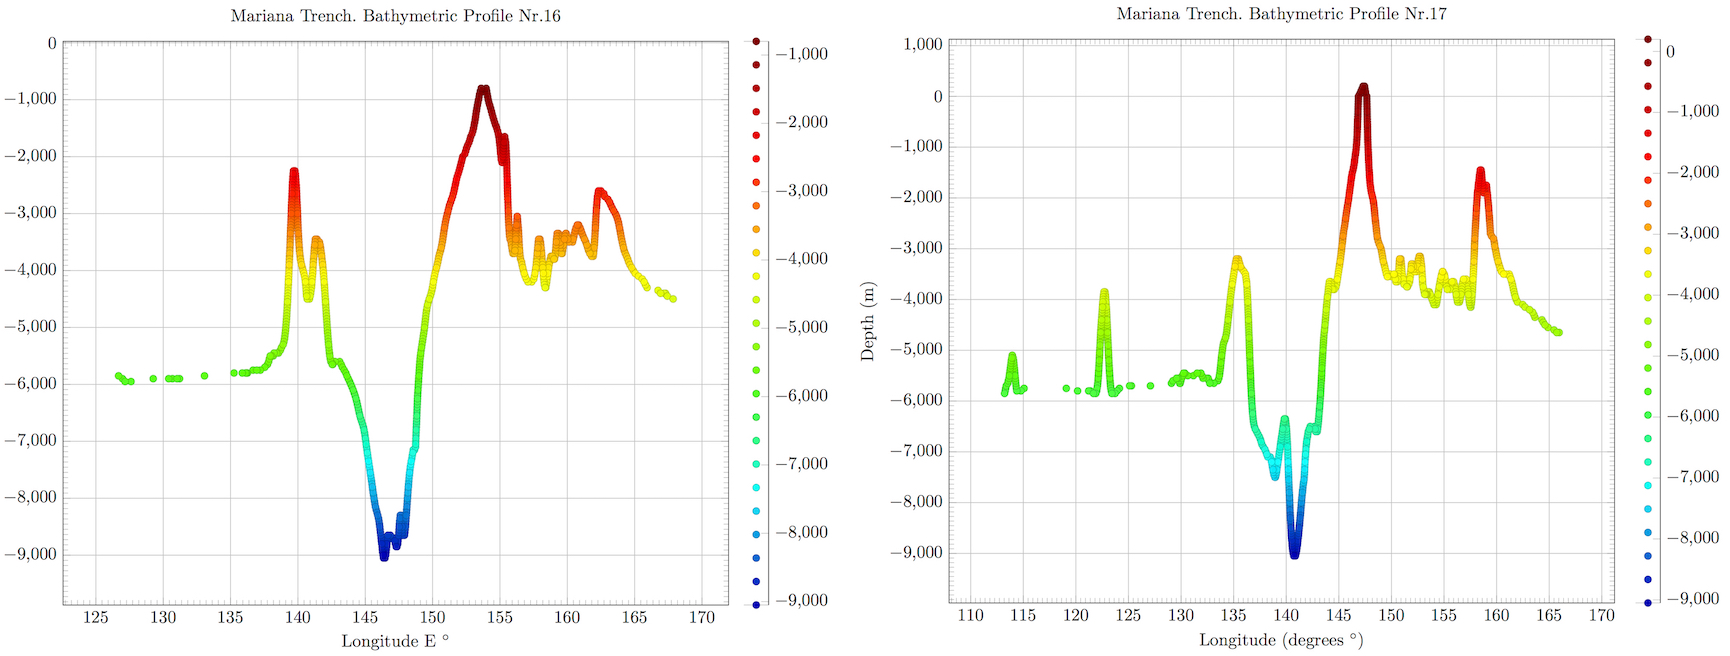
\includegraphics[width=13cm]{Fig-4-2-1.jpg}
	\caption{Selected bathymetric profiles of the Mariana Trench. Plot visualization: \LaTeX}\label{fig:4-2-1}
\end{figure}

\begin{figure}[H]
	\centering
		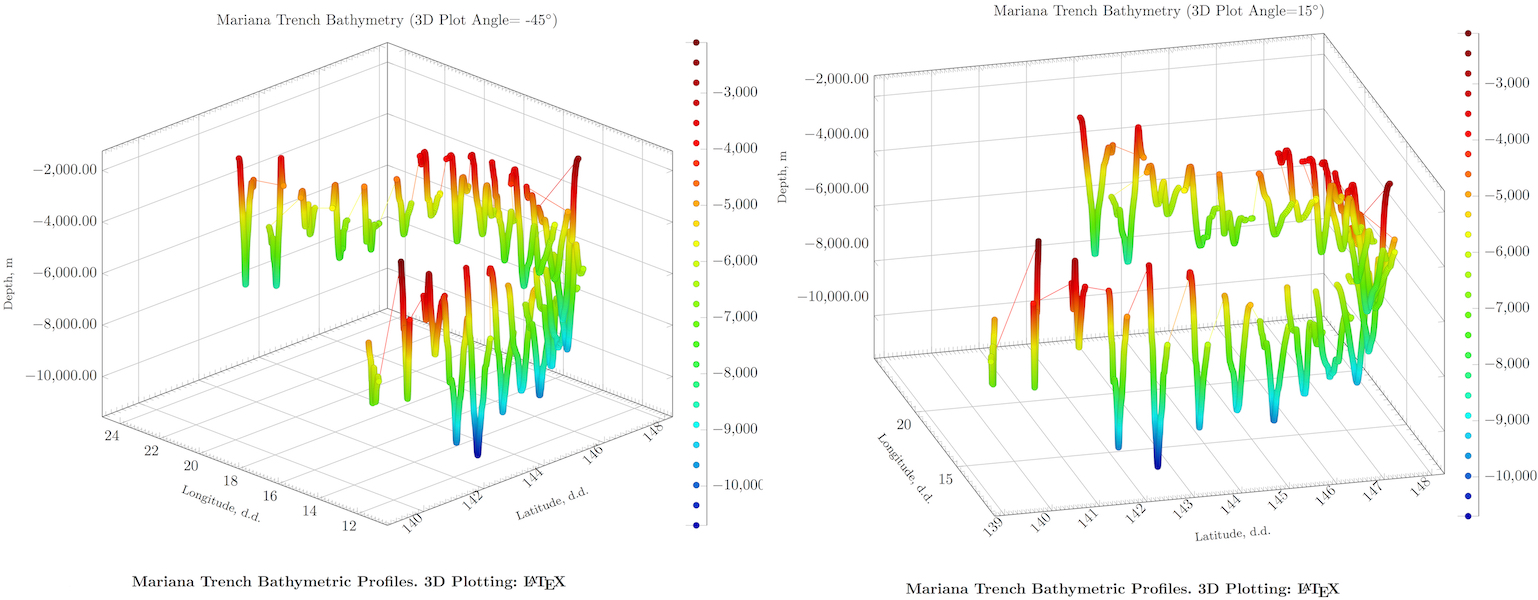
\includegraphics[width=13cm]{Fig-4-2-2.jpg}
	\caption{3D-view of the 25 bathymetric profiles of the Mariana Trench. Plot visualization: \LaTeX}\label{fig:4-2-2}
\end{figure}

%%%%%%%%%%%%%%%%%  Chapter  4: Results%%%%%%%%%%%%

\chapter{Results}\label{chp:4}
	\markright{Results}
	\counterwithin{figure}{section}
	\counterwithin{table}{section}
	
\section{Kuril-Kamchatka Trench}

\subsection{Southern segment of the \ac{KKT}}
Technically, the comparison of the two parts of the trench was performed by means of the set of the cross-section profiles plotted by \ac{GMT} in an automatic regime for northern and southern part of the trench. The morphology of both segments was then compared with aim to identify the characteristics of the trench geomorphology. The summary interpretation of the 52 NE-SW cross-section profiles across the \ac{KKT} in the southern part (highlighted as green line on the Fig. \ref{fig:KKT1}) shows following results. At the southern region (located in the proximity of the active volcanic spots, see Fig. \ref{fig:KKT2}), the seafloor depths are found to decrease with increasing latitude gradually while moving northwards. Trench morphology in the northern termination of the southern segment of the \ac{KKT}, just approaching the Bussol Strait \index[places]{Bussol Strait} is at the U-trending seafloor rise. Besides, there is indication of the slab subduction along the NW margin of the trench facing the Sea of Okhotsk \index[places]{Sea of Okhotsk}. Here the trench-parallel, linear system of the southern part of the Greater Kuril Chain \index[places]{Greater Kuril Chain}: Iturup Island \index[places]{Iturup Island}, Urup \index[places]{Urup Island}, Shikotan \index[places]{Shikotan Island} and minor chain of islands. These islands provide a natural barrier to the extensive downslope sediment transport from the southern Sea of Okhotsk to the trench. To a certain extent, they are trapped behind the chain of islands and further restrict the supply of the sediments to the central part of the trench downslope.

\begin{figure}[H]
	\centering
	\includegraphics[width=10cm]{Fig-KKT4.jpg}
	\caption{Median stacked profiles of the \ac{KKT} with error bars for the southern (A) and northern (B) segments.}\label{fig:KKT4}
\end{figure}

The submarine terraces are presented along the southern part of the trench axis. A common trend is that southern part of the seafloor depths are found to vary considerably, even within neighboring selected profiles. The wedge-shaped body of the trench is being developed in its southern part on the westwards trench slope in front of the Sea of Okhotsk\index[places]{Sea of Okhotsk} inner trench wall closer to the islands Kunashir, Urup and Iturup from the Kuril Greater Chain. It shows a typical and distinct morphologic impact from the nearby subduction zone. The areas of the submarine terraces interspersed with the floodplains have been observed in the southern part of the trench at -4000 m depth forming distinctive patterns on the landforms located immediately southwards the Bussol Strait. The southern part of the KKT near Kuril Basin (Fig. \ref{fig:KKT1}) creates conditions for the short sediment transport from the islands between the terrestrial sediments of the Sakhalin Island \index[places]{Sakhalin Island} and the Kurils with marine sediments sinking to the trench.

\begin{figure}[H]
	\centering
	\includegraphics[width=10cm]{Fig-KKT5.jpg}
	\caption{Enlarged view of the profiles: numbering starts from south to north for both segments.}\label{fig:KKT5}
\end{figure}

In the southern segment, the sedimentation system goes in a transverse direction of the trench stretching: it brings the sediments from the islands located on the south of Sea of Okhotsk\index[places]{Sea of Okhotsk}: Hokkaido, Kunashir \index[places]{Kunashir Island}, Iturup, Urup and minor islands of the southern part of Greater Kuril Chain\index[places]{Greater Kuril Chain}. The southern part of the trench here serves as a sink for the sediment dispersal systems along the active margins of the Kuril Islands. Therefore, it is longitudinally fed by the sediments derived from the southern Kuril. Besides, the location of the compression-extension tectonic slabs as demonstrated on the Fig. \ref{fig:KKT2} and the average deformation of the trench’s axis is directly affected by the source of earthquakes located in the south of the Greater Kuril Chain \index[places]{Greater Kuril Chain}.

\subsection{Northern segment of the \ac{KKT}}
The northern part of the \ac{KKT} (highlighted as red line segment on the Fig. \ref{fig:KKT1}) reflects in its morphological features the combined effects of tectonic slab subduction, collision, and sedimentation processes and closeness of the \ac{LIPs} in the northern part of the Pacific Ocean \index[places]{Pacific Ocean} close to the Bering Sea \index[places]{Bering Sea}. In particular they are being determined by the rate of the Pacific Plate \index[places]{Pacific Plate} convergence, sediment supply, and the topography of the subducting seafloor. Fracture zones oriented in NW direction from the Pacific Plate towards the trench affect the sediment deposition in trench. Namely, the sediment deposits filling the trench are mostly controlled by the rate of the Pacific plate convergence towards Okhotsk Plate\index[places]{Okhotsk Plate}. The analysis and interpretation of the 62 NE-SW cross-section profiles across the \ac{KKT} in the northern part shows following results. 

The sequence of profiles crossing the northern part of the trench show truncated landforms at the canyon walls of the Greater Kuril Chain \index[places]{Greater Kuril Chain}, which rise ca. 1000 m \ac{ASL} while southern part of the islands chain (Iturup and Urup islands) show ca. 400 m \ac{ASL}.  The area around the northern part of the trench identified features of the trench geomorphological system (submarine canyons, trench wedge, submarine ridges, and basins) in the northern part of the trench. The trench-parallel longitudinal sedimentation system carries sediments eroded from the Kamchatka orogenic system to the east, along the Kamchatka Peninsula \index[places]{Kamchatka Peninsula}. These deposits are then moved to the north-eastern part of the trench, shown as red line on Fig. \ref{fig:KKT1}.
The northern part of the \ac{KKT} receives the sediments transported in a southwest direction from the downslopes of the Kamchatka \index[places]{Kamchatka Peninsula}and northern islands. Trench-fill sediments are then mostly derived from the volcanic arcs formed by the Kamchatka Peninsula \index[places]{Kamchatka Peninsula} and northern segment of the Kuril islands, as well as adjacent volcanic basins. From the Kurils the sediments are transported to the northern part of the trench bottom through the set of submarine canyons directed transverse to the axis of the northern \ac{KKT} filling it by terrigenous sediments.

\begin{figure}[H]
	\centering
	\includegraphics[width=10cm]{Fig-KKT6.jpg}
	\caption{Northern part of the geomorphology of the \ac{KKT}: a graph based on the table reshaped by AWK script.}\label{fig:KKT6}
\end{figure}

Orthogonal profiles line Nr. 1 and 7, located north of the \ac{KKT} in perpendicular direction off the Academy of Sciences Rise \index[places]{Academy of Sciences Rise} (Fig. \ref{fig:KKT1}) reveal the steeper shape form caused by the seismic characteristics and sedimentary accumulation patterns of the south-east parts of Sea of Okhotsk \index[places]{Sea of Okhotsk}. The increased number of profiles while moving in northwards direction show shallower depths which illustrates previous discussion on the variations in the sedimentation processes of northern and southern part of the trench, and the landform of the profiles in the respective segments.

\begin{figure}[H]
	\centering
	\includegraphics[width=10cm]{Fig-KKT7.jpg}
	\caption{Southern part of the geomorphology of the \ac{KKT}: a graph based on the table reshaped by AWK script.}\label{fig:KKT7}
\end{figure}

Farther down the trench and north-east of the Shiashkotan Island \index[places]{Shiashkotan Island} from the Kurils, profile line 42 and 49 cross take the form of an irregularly shaped trough of ca. 8 km width. The trench floor morphology here is characterized by the gentle slope patterns and depths not exceeding 7,400 m. On both profiles, the northern wall of the trench is the island-ward sloping surface of the Kuril islands. Profile line 56 shows mainly flat and parallel form at the shallower depths that extend to about 7,200 m in the seafloor. Further profile line 62 shows even more shallower depth and gentle slope shape following the enlargement of the trench valley starting northwards from the Paramushir Island \index[places]{Paramushir Island}. Stacks of local small hills and bulges across the trench indicate multiple sediment deposition processes along the trench slope in its northern part.

\subsection{Comparison of the southern and northern segments}
Comparing northern and southern parts of the trench, the wedge-like or U-shaped morphology of the trench in two parts south- and northwards from the Bussol Strait \index[places]{Bussol Strait} are distinct not only from the inner-ward slope facing the Sea of Okhotsk \index[places]{Sea of Okhotsk} and the Greater Kurils Chain \index[places]{Greater Kurils Chain}, but also in longitudinal direction along the trench axis. This particular may be explained by the response to the gradual changes in seafloor topography patterns. Another impact can be added by the oceanological factors, such as intensive bottom currents. Diverse types of the sediment deposits filling the trench in its northern and southern part differ in substrate content: more volcanic sediments are in the south comparing to the northern part, which can be influenced by the different seismic settings and sediment transport paths. Steeper landforms are in general observed in the southern part of the trench comparing to those in its northern segment. In both southern and northern parts of the trench, the floor deposits are influenced by the lateral and longitudinal sediment supply.\\
The results of the comparative analysis of the two distinct parts of the trench located north- and southwards from the Bussol Strait \index[places]{Bussol Strait} show that southern part is deeper reaching -8,200 m depth while northern part has -7,800 at maximal records. The data analysis was performed to examine the spatial variation of the trench geomorphology including the interrelationships of the factors affecting its variation (geodetic, seismic, geologic and bathymetric). Variations in the earthquakes magnitude and seismisity in the study area that are higher in the south-western part of the trench, as well as to a lesser extent location in the magnetic anomalies located in the north-east, influence the bathymetric patterns that show deeper values in the southern part and geomorphic landforms distribution. The cross-section profiles across the northern part of the \ac{KKT} show deeper values of the depth and less steep slopes comparing to the southern segment, which refer to the erosional moats and drift of the submarine sediments. \\
On the contrary, southern profiles along the trench, comparing to the northern segment, located near the intense volcanic area demonstrate erosional moats at -3000 m depths adjusting the Greater Kuril Chain\index[places]{Greater Kuril Chain}. This reflects a series of recent earthquakes erupted near Shikotan Island \index[places]{Shikotan Island} in the southern part of the \ac{KKT}. Besides, the anomalous metallogeny of the southern Kuril segment is determined by the deep geodynamics, which provided the impact of fluid energy fluxes from sub-subduction and supra-subduction asthenospheric zones. The profiles in the southern segment of the trench show more complex pattern of the processes of erosion along the upper slope and sediment deposition comparing to the northern segment. Therefore, the landward oriented submarine ridges of the trench facing the Greater Kuril Chain \index[places]{Greater Kuril Chain} form oblique landform shape towards the coast of the southern Kurils. Southern part of the trench follows the exposition to the erosion processes in NE to SW direction caused by the intense earthquakes located on the south of the Greater Kuril Chain \index[places]{Greater Kuril Chain}.\\
Northern part of the trench affected by numerous earthquakes located on the Kamchatka Peninsula \index[places]{Kamchatka Peninsula} (see Figure 2) is influenced by the large amount of the accumulated sediments. Necessarily it forms the shallower depths and gentle flat slopes in the morphology of the northern part of the \ac{KKT}. On the contrary, the southern part is presented by V-shape formed slopes and steeper morphology which is affected by the specific geophysical conditions of the southern part of the Kuril Islands characterized by the magnetized anomaly zones of the oceanic crust. The junction of two different segments of the Kuril Islands, southern and northern, corresponds to a sub-latitudinal magnetic anomaly. The north-east direction of the magnetic anomalies are recorded on the oceanic slope of the trench up to its island slope while the southern segment of the trench axis is oriented in parallel. 

\begin{figure}[H]
	\centering
	\includegraphics[width=14cm]{Fig-KKT8.jpg}
	\caption{Statistical 2D histograms and rose diagrams showing comparative depths distribution in the southern and northern part of the \ac{KKT}. Rose diagram shows the aspect of the slopes}\label{fig:KKT8}
\end{figure}

The orthogonal bathymetric profiles across the southern and northern segments of the \ac{KKT} identify two distinct U- and V-shaped morphologic features with affecting dominant processes: (1) in its northern segment, the dominant processes along the Kamchatka Peninsula are sediment deposition; (2) southern part located near the Hokkaido \index[places]{Hokkaido Island}, Iturup \index[places]{Iturup Island} and Urup \index[places]{Urup Island} islands and minor island of the Greater Kuril Chain are distinct by the processes of erosion and intense sediment transportation. The explosive volcanism in different parts of the \ac{KKT} explain a high mass of sediments formed by gradual sediment accumulation.
	
\section{Aleutian Trench}

The \ac{GMT} based modelling demonstrated following results. The topography in the study area ranges between -8200 to 2000 m (Fig. \ref{fig:A6}). The geoid gravitational model shows the majority of values lies in the interval between -10 to 20 mGal with the lowest values along the trench. The profiles plotted in an automated regime are located with a distance of 20 km between each pair, spaced every 2 km along the profiles itself and have a total length of 400 km, that is 200 km to both sides from the trench. According to the statistical histogram modelling, the most often depth value in the study area is - 4800 with frequency 1722. The derived cross-section profiles on a selected segment of the trench (a map on Fig. \ref{fig:A6}) includes a combination of the \ac{ETOPO1} bathymetric map with a set of the automatically drawn profiles (Fig. \ref{fig:A6}, lower part), and a statistical visualization of the median stacked profiles with error bars (Fig. \ref{fig:A6}, graph on the upper part).
 
 \begin{figure}[H]
	\centering
		\includegraphics[width=13cm]{Fig-A6.jpg}
	\caption{Automatic digitizing cross-section profiles on the selected segment of the study area}\label{fig:A6}
\end{figure}

 Four approaches for the profile linear trend modelling were tested. Finally, a surface modelling was performed using xyz modelling from the \ac{ASCII} data. The results of this study demonstrated (Fig. \ref{fig:A10}) distribution of the local occurrence of bathymetric data along the cross-section profiles. Visualizing submarine geomorphology provided context and guidance for further geological and oceanographic discussions regarding hadal trench shape, occurrence of terraces, steepness of the slopes, location of canyons, as well as their distribution.
 
\begin{figure}[H]
	\centering
		\includegraphics[width=13cm]{Fig-A7.jpg}
	\caption{Modelling trends for the relief of the mean cross-section profile}\label{fig:A7}
\end{figure}

The bathymetry was visualized using ‘geo’ color palette. The original data is derived from the sea-surface satellite altimetry measurements and ocean soundings provided by numerous global geospatial sources. Therefore, the \ac{ETOPO1} includes existing bathymetry data and uses interpolated gravity values elsewhere. The statistical inventory of the bathymetric data shown (Fig. \ref{fig:A8}) that depths with ranges between -5600 and -5400 m have occurrence of 1106 (8\%); depths with ranges between -5400 and -5200 m have occurrence of 846 (7\%); depths with ranges between -4900 and -5200 m have occurrence of 1297 (11\%). The highest values demonstrated values of -4900 and -4700 with 1722 occurrences (13,2\%). Significantly low values demonstrated shallow areas with depth ranges between -4500 and -3000 m with occurrence of below 200 (all of then less than 2,5\%). Values with ranges shallower than -500 m naturally belong to the coastal shelf areas near the Aleutian Islands adjusting the trench. 

\begin{figure}[H]
	\centering
		\includegraphics[width=13cm]{Fig-A8.jpg}
	\caption{Histogram chart showing bathymetric data distribution by profiles}\label{fig:A8}
\end{figure}

Furthermore, a geomorphic analysis (Fig. \ref{fig:A7} and Fig. \ref{fig:A3}) shown that the north-western part of the trench on the side of the chain of islands has steeper and shorter slope, with located series of marine terraces.
Several present models and maps describe the geological, geophysical and geomorphic modelling of the study area including an outline of the shell scripting, the model, and visualized maps. To assist in the identification of the geomorphology of the Aleutian trench, the bathymetric \ac{ETOPO1} data were contoured at 500 m intervals using GMT module ‘grdcontour’ (Fig. \ref{fig:A2}). 

\begin{figure}[H]
	\centering
		\includegraphics[width=10cm]{Fig-A9.jpg}
	\caption{Topographic surface modelling from the ASCII xyz data}\label{fig:A9}
\end{figure}

The geomorphic analysis process in GMT module ‘trend1d’ was applied to build statistical trends with four functional approaches (Fig. \ref{fig:A7}) and well as visualization of median and mean profiles (Fig. \ref{fig:A6}). The results of the surface modelling (Fig. \ref{fig:A9} and Fig. \ref{fig:A10}) were used by modelling xyz dataset. 

\begin{figure}[H]
	\centering
		\includegraphics[width=10cm]{Fig-A10.jpg}
	\caption{Surface modelling from the ASCII xyz data}\label{fig:A10}
\end{figure}
	
\section{Middle America Trench}
The output model of the cross-section profiles is provided at Figure \ref{fig:MAT10} showing the initial bathymetric map (Figure \ref{fig:MAT10} B) and above a plotted series of the profiles (Figure \ref{fig:MAT10} A), such as oceanward backers of the trench and more steeper slope on the continental side. 


\begin{figure}[H]
	\centering
		\includegraphics[width=13cm]{Fig-MAT10.jpg}
	\caption{Cross-section profiles on the selected segment of the \ac{MAT}. The computations were done using GMT modules by the code provided in Appendix}\label{fig:MAT10}
\end{figure}

However, other areas, particularly the terraces were less well defined, perhaps due to the local specific geomorphic features of the study object: the geomorphology of the \ac{MAT} presents a very straight steep slopes without significant curvatures. Multiple factors affect \ac{MAT} geomorphology which is formed as a results of the complex interaction between the geochemical situation, lithology, sedimentation processes, geological trigger factors and tectonic mechanisms in the study area. These factors include include among others tectonic history of the study area, strong influence of the volcanic active zone, geochemical content of the substrate. The position of the bathymetric observations in the trend analysis (Fig. \ref{fig:MAT11}, A) indicates the main common trend similarities in the sea floor characteristics between the geomorphic units. Thus, Fig. \ref{fig:MAT11}, A shows clear separation of the oceanward slope with steeper angle Cocos Plate basin, trench valley and rocky Charts block unit. 

\begin{figure}[H]
	\centering
		\includegraphics[width=10cm]{Fig-MAT11.jpg}
	\caption{Trend regression models for the cross-section profiles, \ac{MAT}. The computations were done using GMT modules by the code provided in Appendix}\label{fig:MAT11}
\end{figure}

Modelling geospatial data highlited the geomorphology and geometric shape of the trench. The geometry of the trench demonstates its relatively steep and strait shape which correlate with previous seismic record results \cite{Shipboard1982500} showing the trench floor to be 3-5 km wide. The spatial analysis performed by the GMT revealed that major depth observation points of the \ac{MAT} are located in between the -3000 and -6200 meters (Fig. \ref{fig:MAT10} and Fig. \ref{fig:MAT11}). Frequency data distribution of the bathymetric samples shows notable changes within the \ac{MAT} by the profiles. There is a certain increase of frequency in depths between -3000 and -4000 m (Fig. \ref{fig:MAT12}) that may be caused by the specific geologic properties of the Cocos Plate. 

\begin{figure}[H]
	\centering
		\includegraphics[width=12cm]{Fig-MAT12.jpg}
	\caption{Histograms of the sample data distribution by the cross-section profiles}\label{fig:MAT12}
\end{figure}

The deepest bathymetry data range with 1,111 records takes 25\% of the total pool of the sample observation points. As can be seen on Fig. \ref{fig:MAT12}, right, the mean values of the observation samples have a value of -2,200, while LMS mode indicates 7,5\% of values at -4,000 to -3,500 m, and median values have values of -3,200 to -3,300 m. The North-West distribution of the rose diagram (Fig. \ref{fig:MAT12}, left) shows steep slope on the oceanward forearc of the trench with relatively few observation samples due to the steepness on the continental slope with denser samples on the Cocos Plate where the geomorphology has more gentle form that can also be noted on (Figure \ref{fig:MAT10}, A). A geoid gravitation model differs significantly by movements in a south-east direction along the study area with clearly detected stripe of the Pacific Volcanic Chain (Fig. \ref{fig:MAT4}). \\
The maximal values of the gravity above 20 mGal are recorded in the south-eastern part of the region southwards Nicaragua \index[places]{Nicaragua}: Nicoya Peninsula \index[places]{ Nicoya Peninsula} and Costa-Rica \index[places]{Costa-Rica} (colored red on the modeled map). The area of Nicaragua has mainly values of 5-15 mGal (colored orange on the modeled map). The area of Gulf of Tehuantepec has the lowest detected gravity values in the range of -15 to -25 mGal (Fig. \ref{fig:MAT4}). The results furthermore indicate that marine vertical gravity at the \ac{MAT} are clearly connected with the trench tectonics correlating with contours of the major lines of tectonic slabs. The intermediate values (20-30 mGal) are locate on the trench slopes (colored orange on the Fig. \ref{fig:MAT6}), while the highest values are detected mainly on the mountainous areas (colored rose on the Fig. \ref{fig:MAT6}). The findings suggest that submarine geomorphic structure of the \ac{MAT} has straight shape form of the slopes with more steep slope on the oceanward forearc. 

\section{Peru-Chile Trench}

\section{Kermadec Trench}
The resulting profiles are visualized as two segments (red and green for both trenches) on Fig. \ref{fig:TK2}, left. Automatic digitizing of the cross-section profiles for Kermadec and Tonga trenches demonstrated that Tonga trench’s geomorphology has steeper gradient slope on the western flank (Fig. \ref{fig:TK3}, A). On the contrary, Kermadec Trench (Fig. \ref{fig:TK3}, B) has more gentle shape form of the western slope off Tonga Ridge \index[places]{Tonga Ridge}. 

\begin{figure}[H]
	\centering
		\includegraphics[width=13cm]{Fig-TK-3.jpg}
	\caption{Geomorphological modelling of the trenches by GMT}\label{fig:TK3}
\end{figure}

The results of the comparative analysis of the two trenches show that Kermadec Trench has more abrupt shape with 2,641 depth records from -6,600 to -6,800 meters (Fig. \ref{fig:TK5}). Comparing the deepest values >9,000 meters for the Kermadec Trench there are 10, 18, 48, 72 and 103, which gives together 251 observation samples proving that Tonga Trench is deeper than Kermadec Trench. If we compare the variations of the seafloor depths at range from -6,000 to -5,000, it can be sen (Fig. \ref{fig:TK5}) that Kermadec Trench has more values in this range: 1820, 2641, 1203 and 503 giving together 6167 samples. The Kermadec has more gentle slope and shallower depths which can also be seen on Fig. \ref{fig:TK3}. This illustrates tectonic and geological local variations, as well as different sedimentation of the Kermadec and Tonga trenches causing variations in their geomorphic shape despite their close location to each other.

\section{Tonga Trench}
The results of the comparative analysis of the two trenches show that Tonga Trench has shallower depths comparing to the Kermadec. Comparing the deepest values >9,000 meters for Tonga Trench there are 5, 39, 72, 95, 109 observations, that sums together 320 samples. Comparing the variations of the seafloor depths at range from -6,000 to -5,000, it can be sen (Fig. \ref{fig:TK5}) that Tonga Trench has 4803 numbers of samples (a sum of 1221, 2089, 1019 and 544).

\begin{figure}[H]
	\centering
		\includegraphics[width=13cm]{Fig-TK-4.jpg}
	\caption{Mathematical approximation of the Kermadec and Tonga trend curves of the profiles}\label{fig:TK4}
\end{figure}

 The results show deeper bathymetry and more seafloor roughness for the Tonga Trench \index[places]{Tonga Trench}. Hence, comparing to the Kermadec, Tonga Trench \index[places]{Tonga Trench} has steeper gradient of the profiles. 
 
\begin{figure}[H]
	\centering
		\includegraphics[width=13cm]{Fig-TK-5.jpg}
	\caption{Histograms of the bathymetry: frequency of the distribution of depths by data for both trenches. Left: Kermadec, right: Tonga}\label{fig:TK5}
\end{figure}

\section{New Hebrides Trench}

\section{Bougainville-New Britain Trench}

\section{Philippine Trench}
The cross-sectional profiles give the insight to the variations in the geomorphological shape of the Philippine Trench and archipelago (Fig. \ref{fig:GML2}). 

\begin{figure}[H]
	\centering
		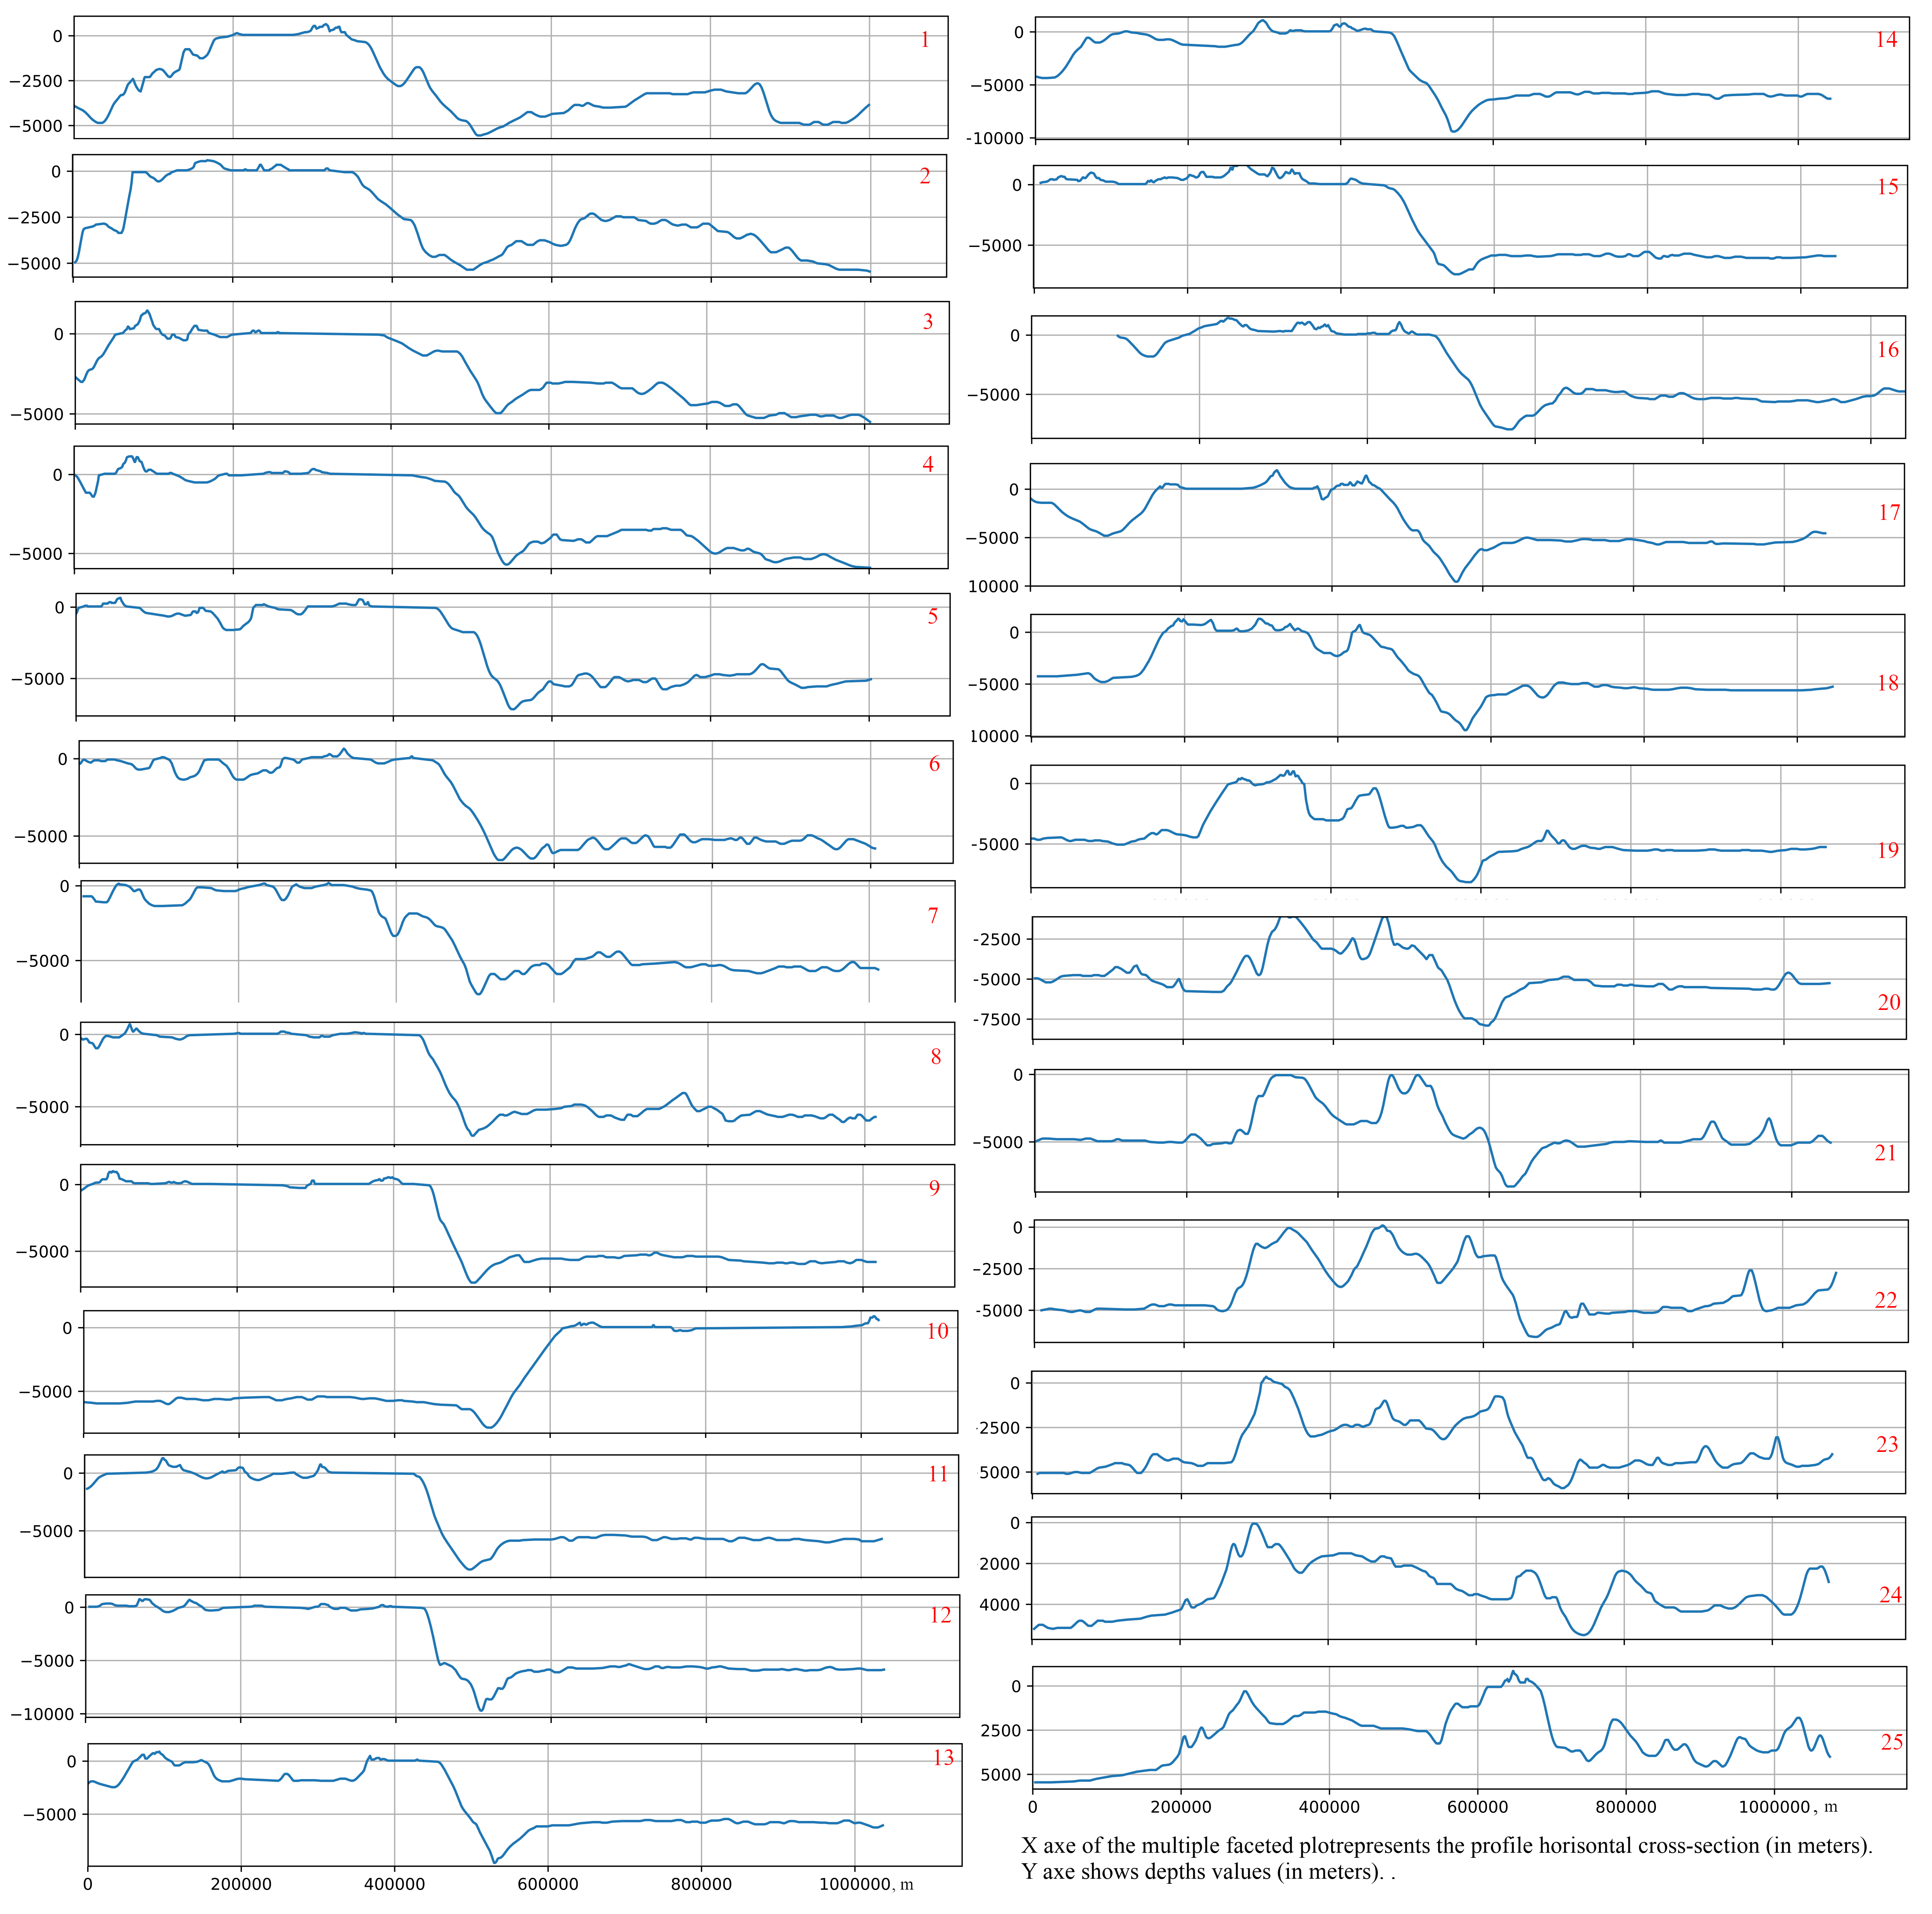
\includegraphics[width=13cm]{Fig-GML2.jpg}
	\caption{Faceted plot of the 25 profiles crossing the Philippine Trench area. Plotting: \ac{QGIS}}\label{fig:GML2}
\end{figure}

The results obtained by different statistical approaches performed using R and Python libraries are analyzed and integrated in order to provide a more detailed understanding of the character of the geomorphic structure of the Philippine Trench. The extreme depths values in the data set are notable for the following profiles: profile Nr. 12 (max depth: -9.700 meters), profile Nr. 13 (max depth: -9.600 m), profile Nr. 14 (max depth: -9.400 m), profile Nr. 18 (max depth: -9.450 m). All these profiles are cross sectioning the Philippine Trench in its central part where its geomorphic pattern can be characterized from ‘steep slope’ (profiles Nr. 12 and 13, see Fig. \ref{fig:GML10}) to ‘very steep slopes’ (profiles 14 and 18). Other profiles have depths not exceeding 9.000 meters.\\
The strip plots (Fig. \ref{fig:GML7}) comprise two visualized relationship types of the data distribution, namely by seven types of the underlie geology with code given and explained in Table 1 (Fig. \ref{fig:GML7}, A) and two tectonic plates: Sunda Plate  \index[places]{Sunda Plate} and Philippine Plate \index[places]{Philippine Plate} (Fig. \ref{fig:GML7}, B). The distribution of the samples across the two tectonic plates is uneven (Fig. \ref{fig:GML7}, A). The Philippine Plate comprise more samples located in the Philippine Sea  \index[places]{Philippine Sea} eastwards from the Philippine Trench. The maximal sampling can bee seen on the profiles 21, 22 and 23 in the southern part of the cross-sectioning (as shown on the map on Fig. \ref{fig:GML1}) with 765, 651 and 652 taken samples, respectively. This is explained by the complex submarine landforms in the western part of the Philippine Sea (Fig. \ref{fig:GML2}, the cross section profiles). Profiles 1-4 demonstrate (Fig. \ref{fig:GML7}, A) significantly lower density of the observation samples not exceeding 200. This part of the section is located in the northern part of the Philippine Trench and is characterized gentle landforms of the submarine geomorphology. 

\begin{figure}[H]
	\centering
	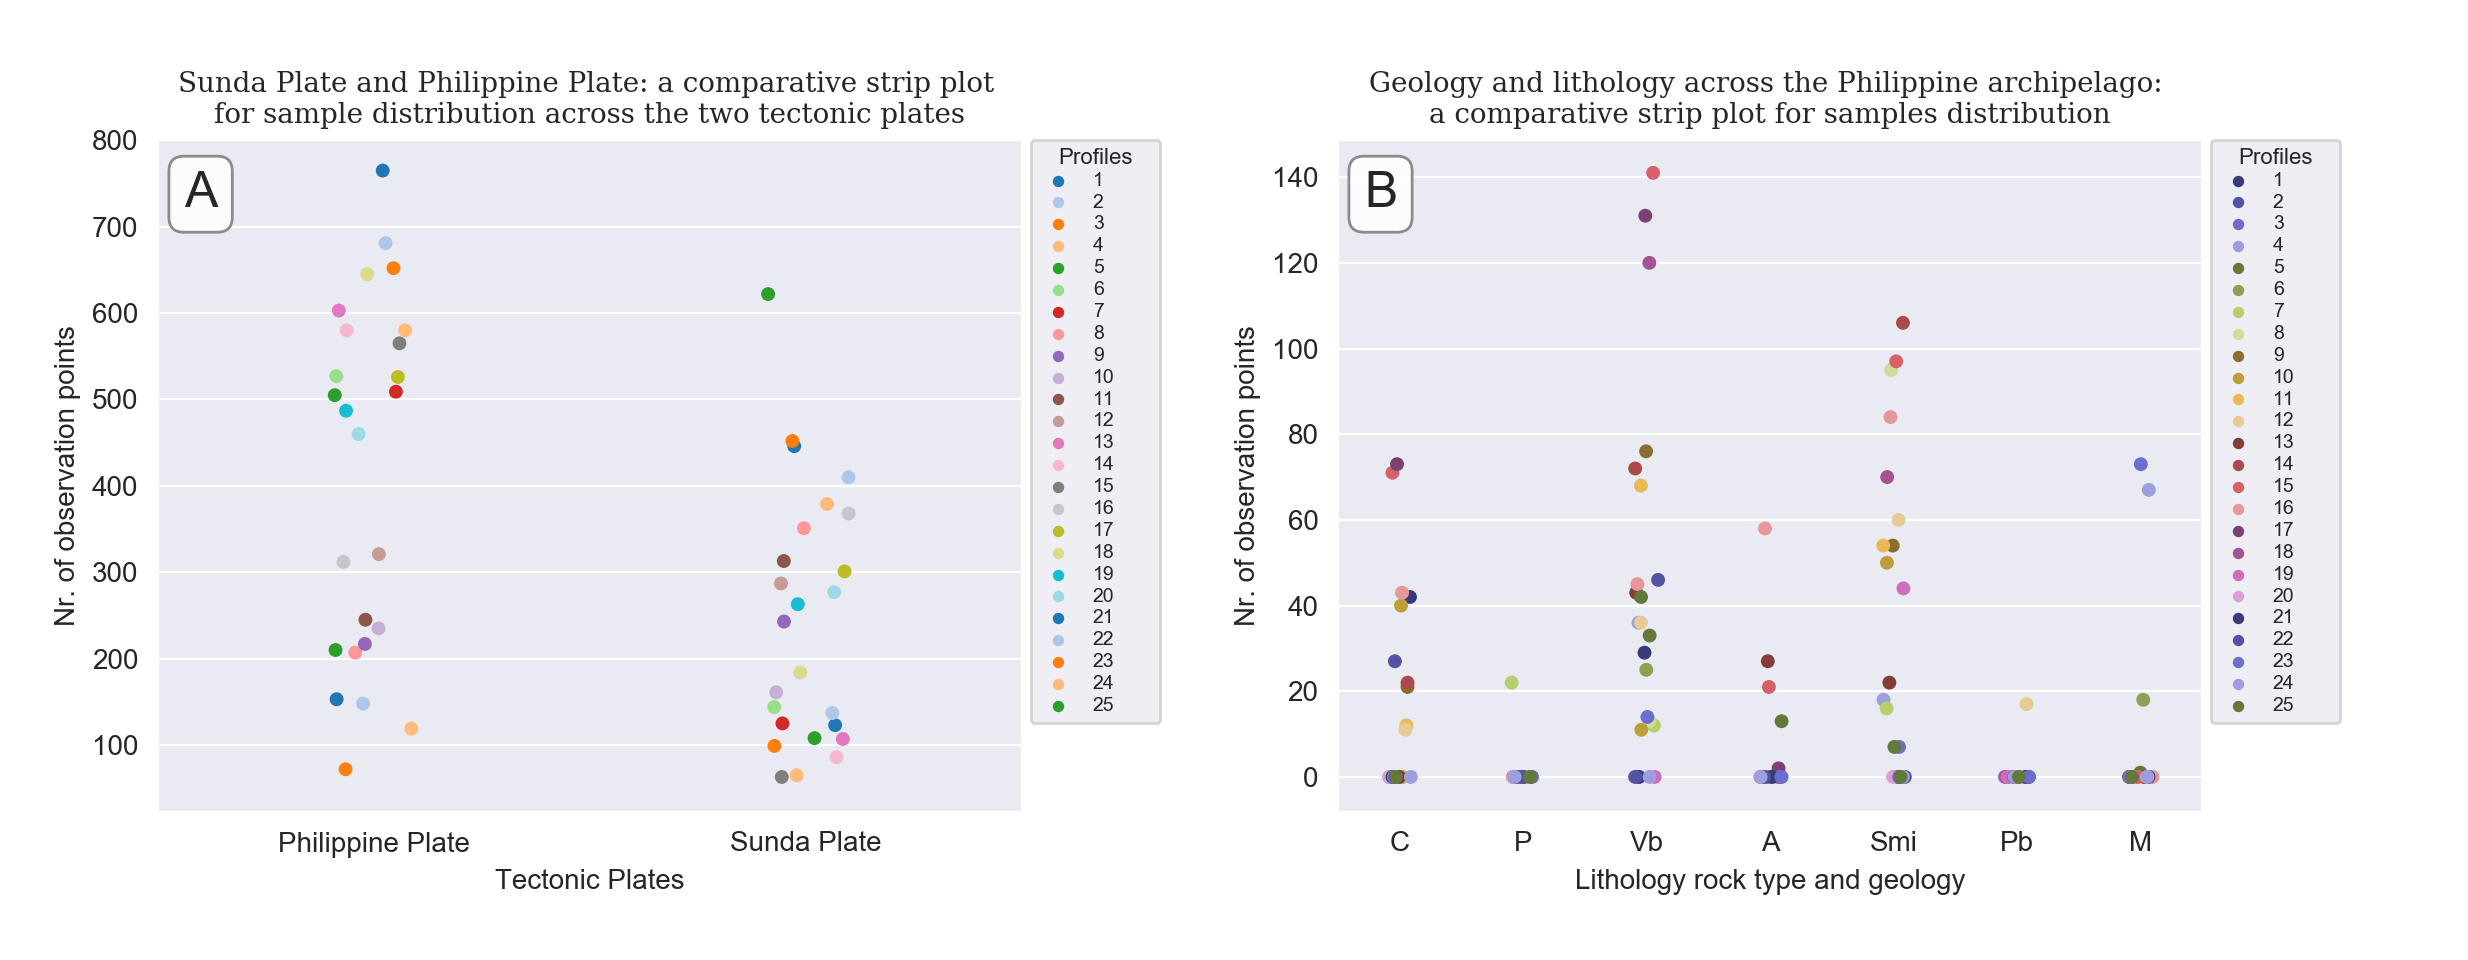
\includegraphics[width=13cm]{Fig-GML7.jpg}
	\caption{Strip plots showing data distribution across tectonic plates (A) and geology (B). Plotting: Python code \ref{P:05}}\label{fig:GML7}
\end{figure}

As can be seen from the Fig. \ref{fig:GML7} (B), the Precambrian \index[concepts]{Precambrian, period} (shield) rocks (P) are only present in profiles 5, 7, 24 and 19 and do not exist in the sample sets of other profiles. South tended data distribution is characterized for lithology types basic-ultrabasic plutonic rocks (Pb) \index[concepts]{Ultrabasic rocks} where data are recorded for the profiles Nr. 12, 18-19, 21, 23-25, that is on the southern part of the Philippine archipelago. The metamorphic rocks (M) are noted across the profiles 23-25, 4, 6, 15-16, that is their distribution is more evenly spread across the study area. In our study, data with complex lithology of Mesozoic \index[concepts]{Mesozoic, period}, Jurassic \index[concepts]{Jurassic, period} and Cretaceous \index[concepts]{Cretaceous, period} origin (C) and Metamorphic rocks (M) \index[concepts]{Metamorphic rocks} have comparable spatial heterogeneity with observation records not overcoming 80 sample observation points. On the contrary, basic volcanic rocks of the Cenozoic \index[concepts]{Cenozoic, Era} volcanic formations (Vb) have significantly higher values reaching maximal values at profiles 18, 17 and 15 having values of 120, 131 and 141 registered samples, respectively. \\
Mixed sedimentary consolidated rocks of Cenozoic formation (Smi) had the highest detected values at profile 14 with 106 recorded points following by profile 8 (95 recorded samples). Finally, alluvial deposits of the Quaternary \index[concepts]{Quaternary, period} have the highest data density recorded at profiles 16 (58 samples), following below by profile 13 and 15 (27 and 21 samples, respectively), that is the central part of the Philippines crossing the archipelago in the shelf area (Fig. \ref{fig:GML7}, B).
 The distribution of the sample points across the Philippine Trench has four distinct groups with the increased values caused by the steep pattern in the geomorphology (Fig. \ref{fig:GML8}, B): first group include profiles Nr. 5, 6, and 7 (northern part of the Philippine Trench crossing further Manila Trench. Second group comprises a group of profiles Nr. 13, 14 and 15: central transect of the Philippine Trench moving westwards towards the Negros Trench \index[places]{Negros Trench}. Third part includes two profiles Nr.  17 and 18. Finally, fourth part includes profiles Nr. 21, 22, 23, 24, that is a southern part of the Philippine Trench where the transects move further crossing Sulu Trench \index[places]{Sulu Trench} and Cotabato Trench \index[places]{Cotabato Trench} on the block of Sunda tectonic plate. 
	
\begin{figure}[H]
	\centering
	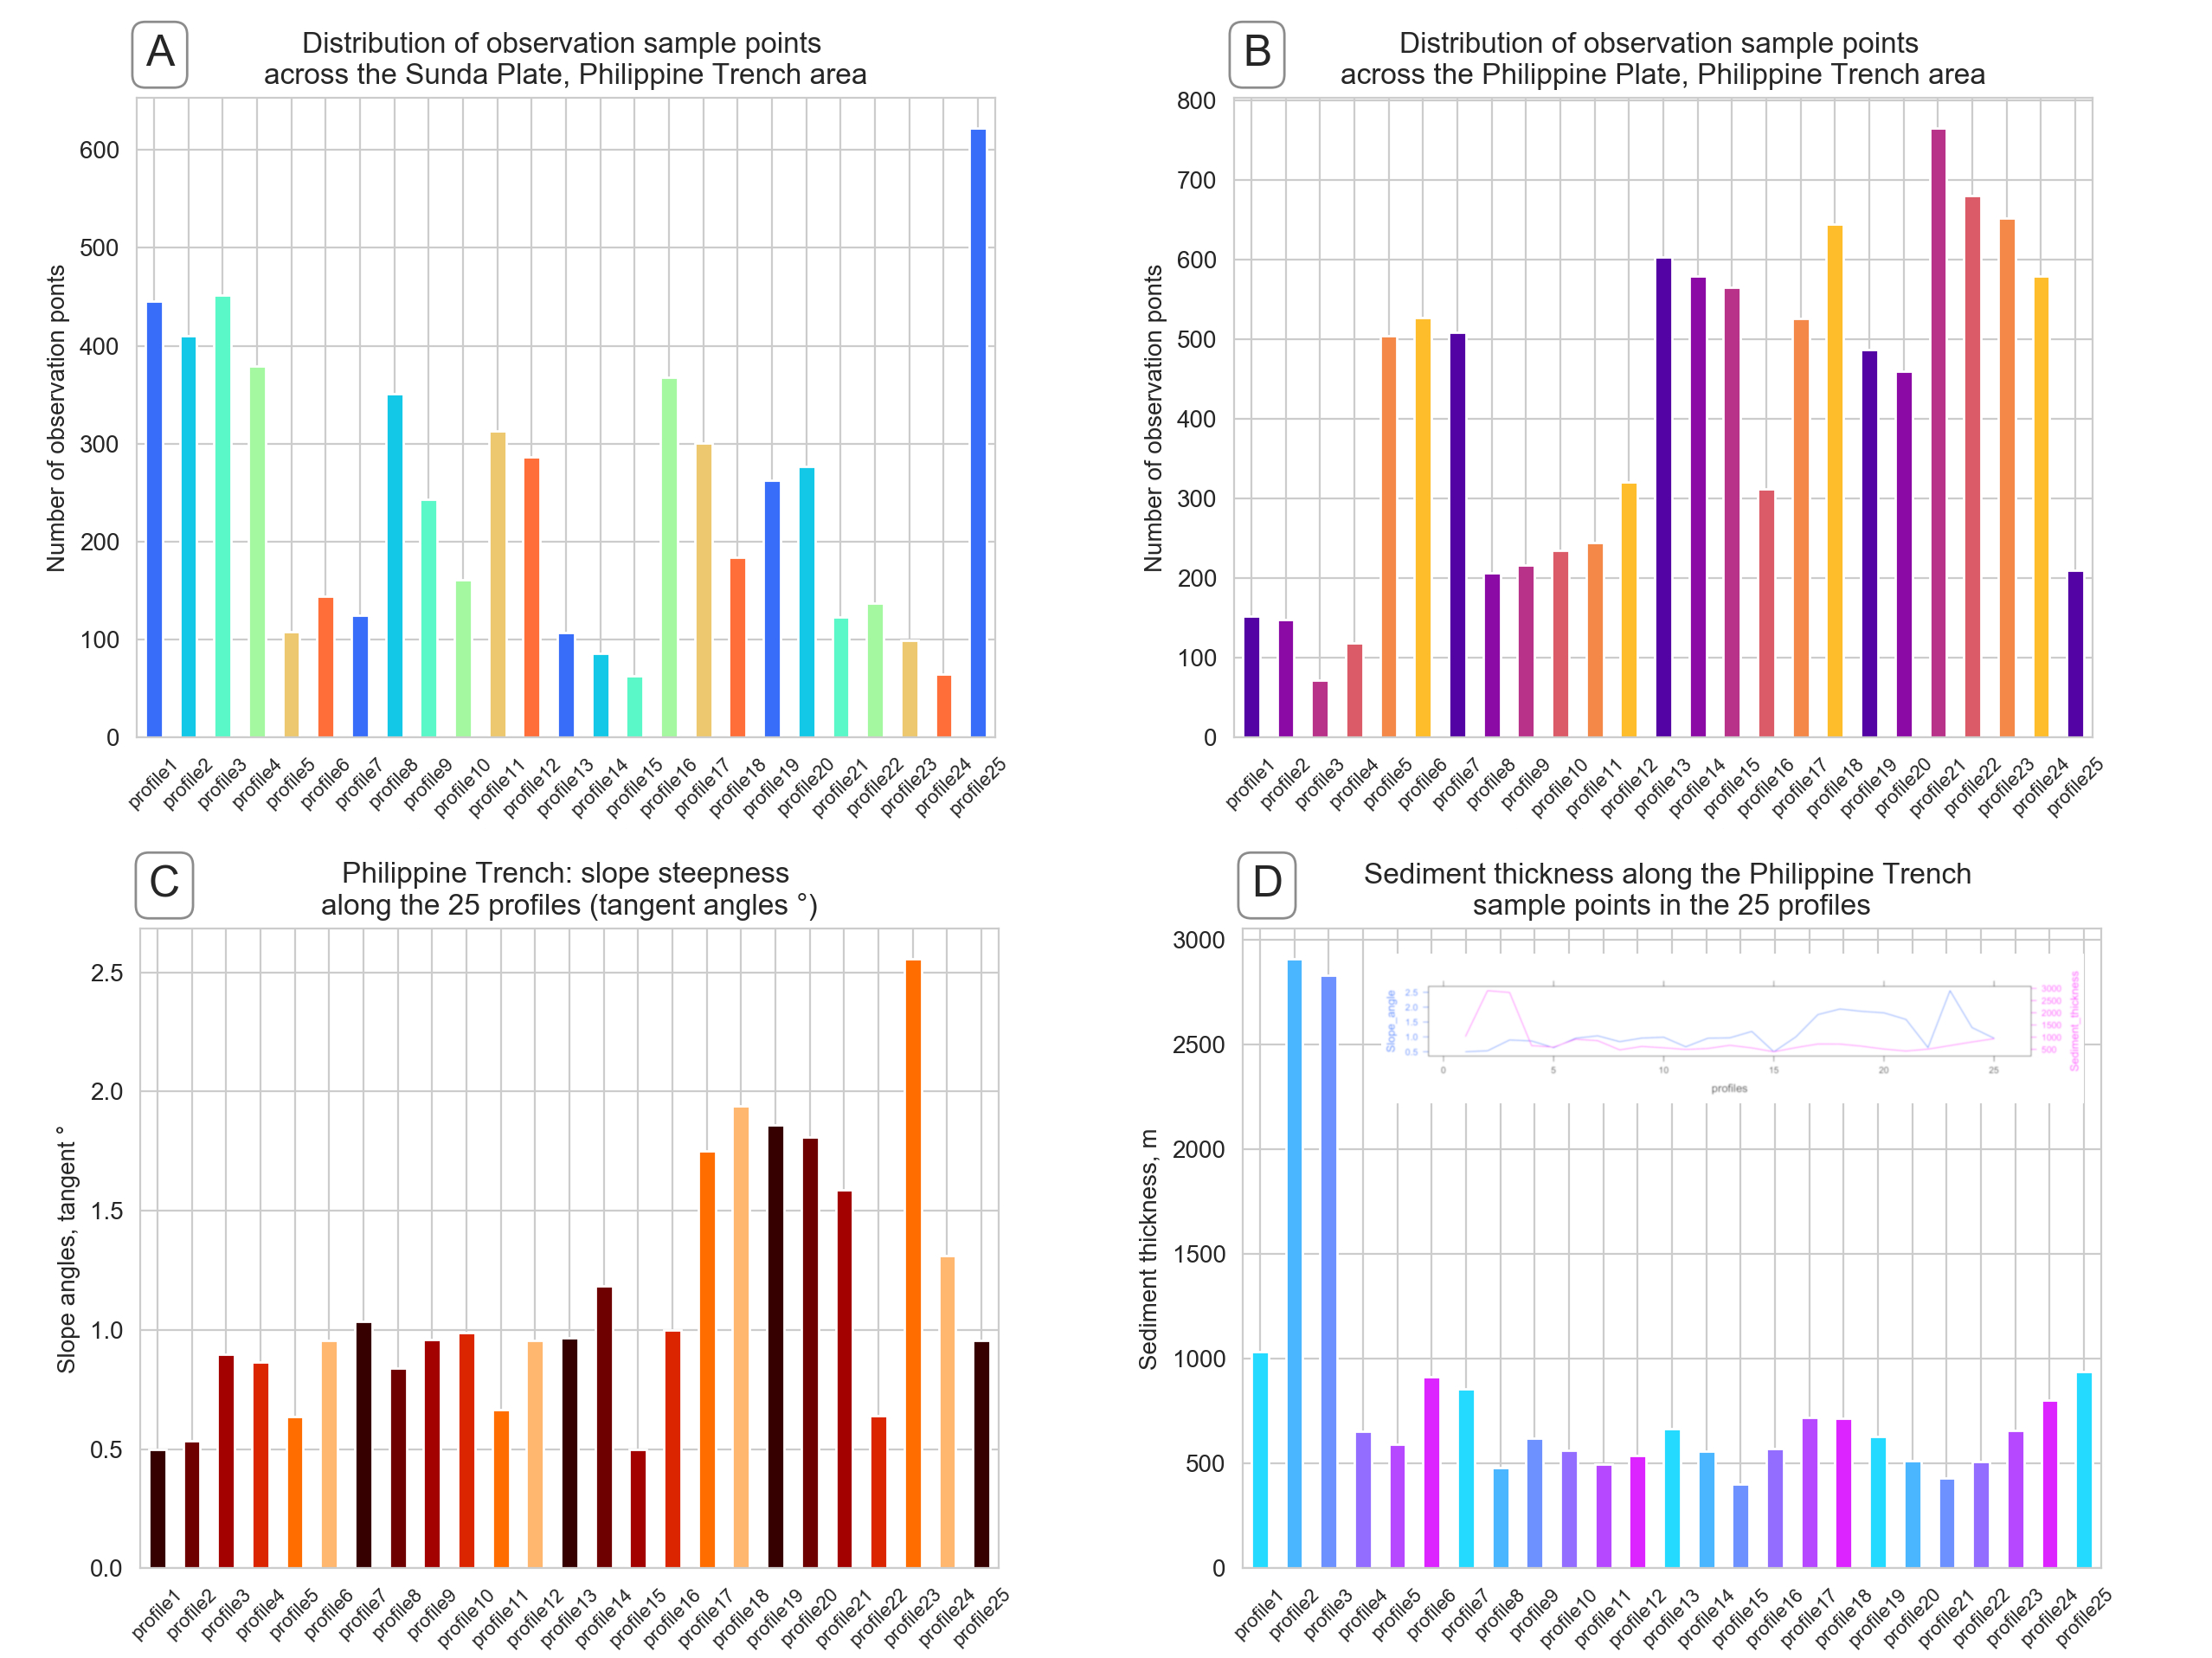
\includegraphics[width=13cm]{Fig-GML8.jpg}
	\caption{Distribution of the sampling points from the cross-section profiles across the tectonic plates. Plotting: Python, Matplotlib library and R (Small subplot in 'D' showing correlation between sediment thickness and slope angles across the 25 cross-section profiles).}\label{fig:GML8}
\end{figure}

The opposite distribution can be seen for the Sunda Plate (Fig. \ref{fig:GML8}, A): profiles 1-4 (northern Sunda) have increased values, followed by the second group of profiles (8-12), then third group (profiles 16-17 and 19-20) and finally, profile Nr. 25 with maximal value for the Sunda Plate. The sediment thickness has a relatively even distribution for all the profiles, which is previously described by \cite{Hessleretal1978} who pointed that the sedimentation in the Philippine Trench is not significantly high to fill in the axis along the trench. However, the exception have profiles Nr. 2 and 3 with a distinct rise in the sedimentation volume caused by the geologic conditions of the Philippine Trench sedimentation \cite{Larsen1968} (Fig. \ref{fig:GML8}, D). South-eastern part of the Philippine Trench (profiles 17-21) has a distinct steeper geomorphic shape (Fig. \ref{fig:GML8}, C) which is caused by the complex relationship between the tectonic slabs and geological settings in this area.  

\begin{figure}[H]
	\centering
	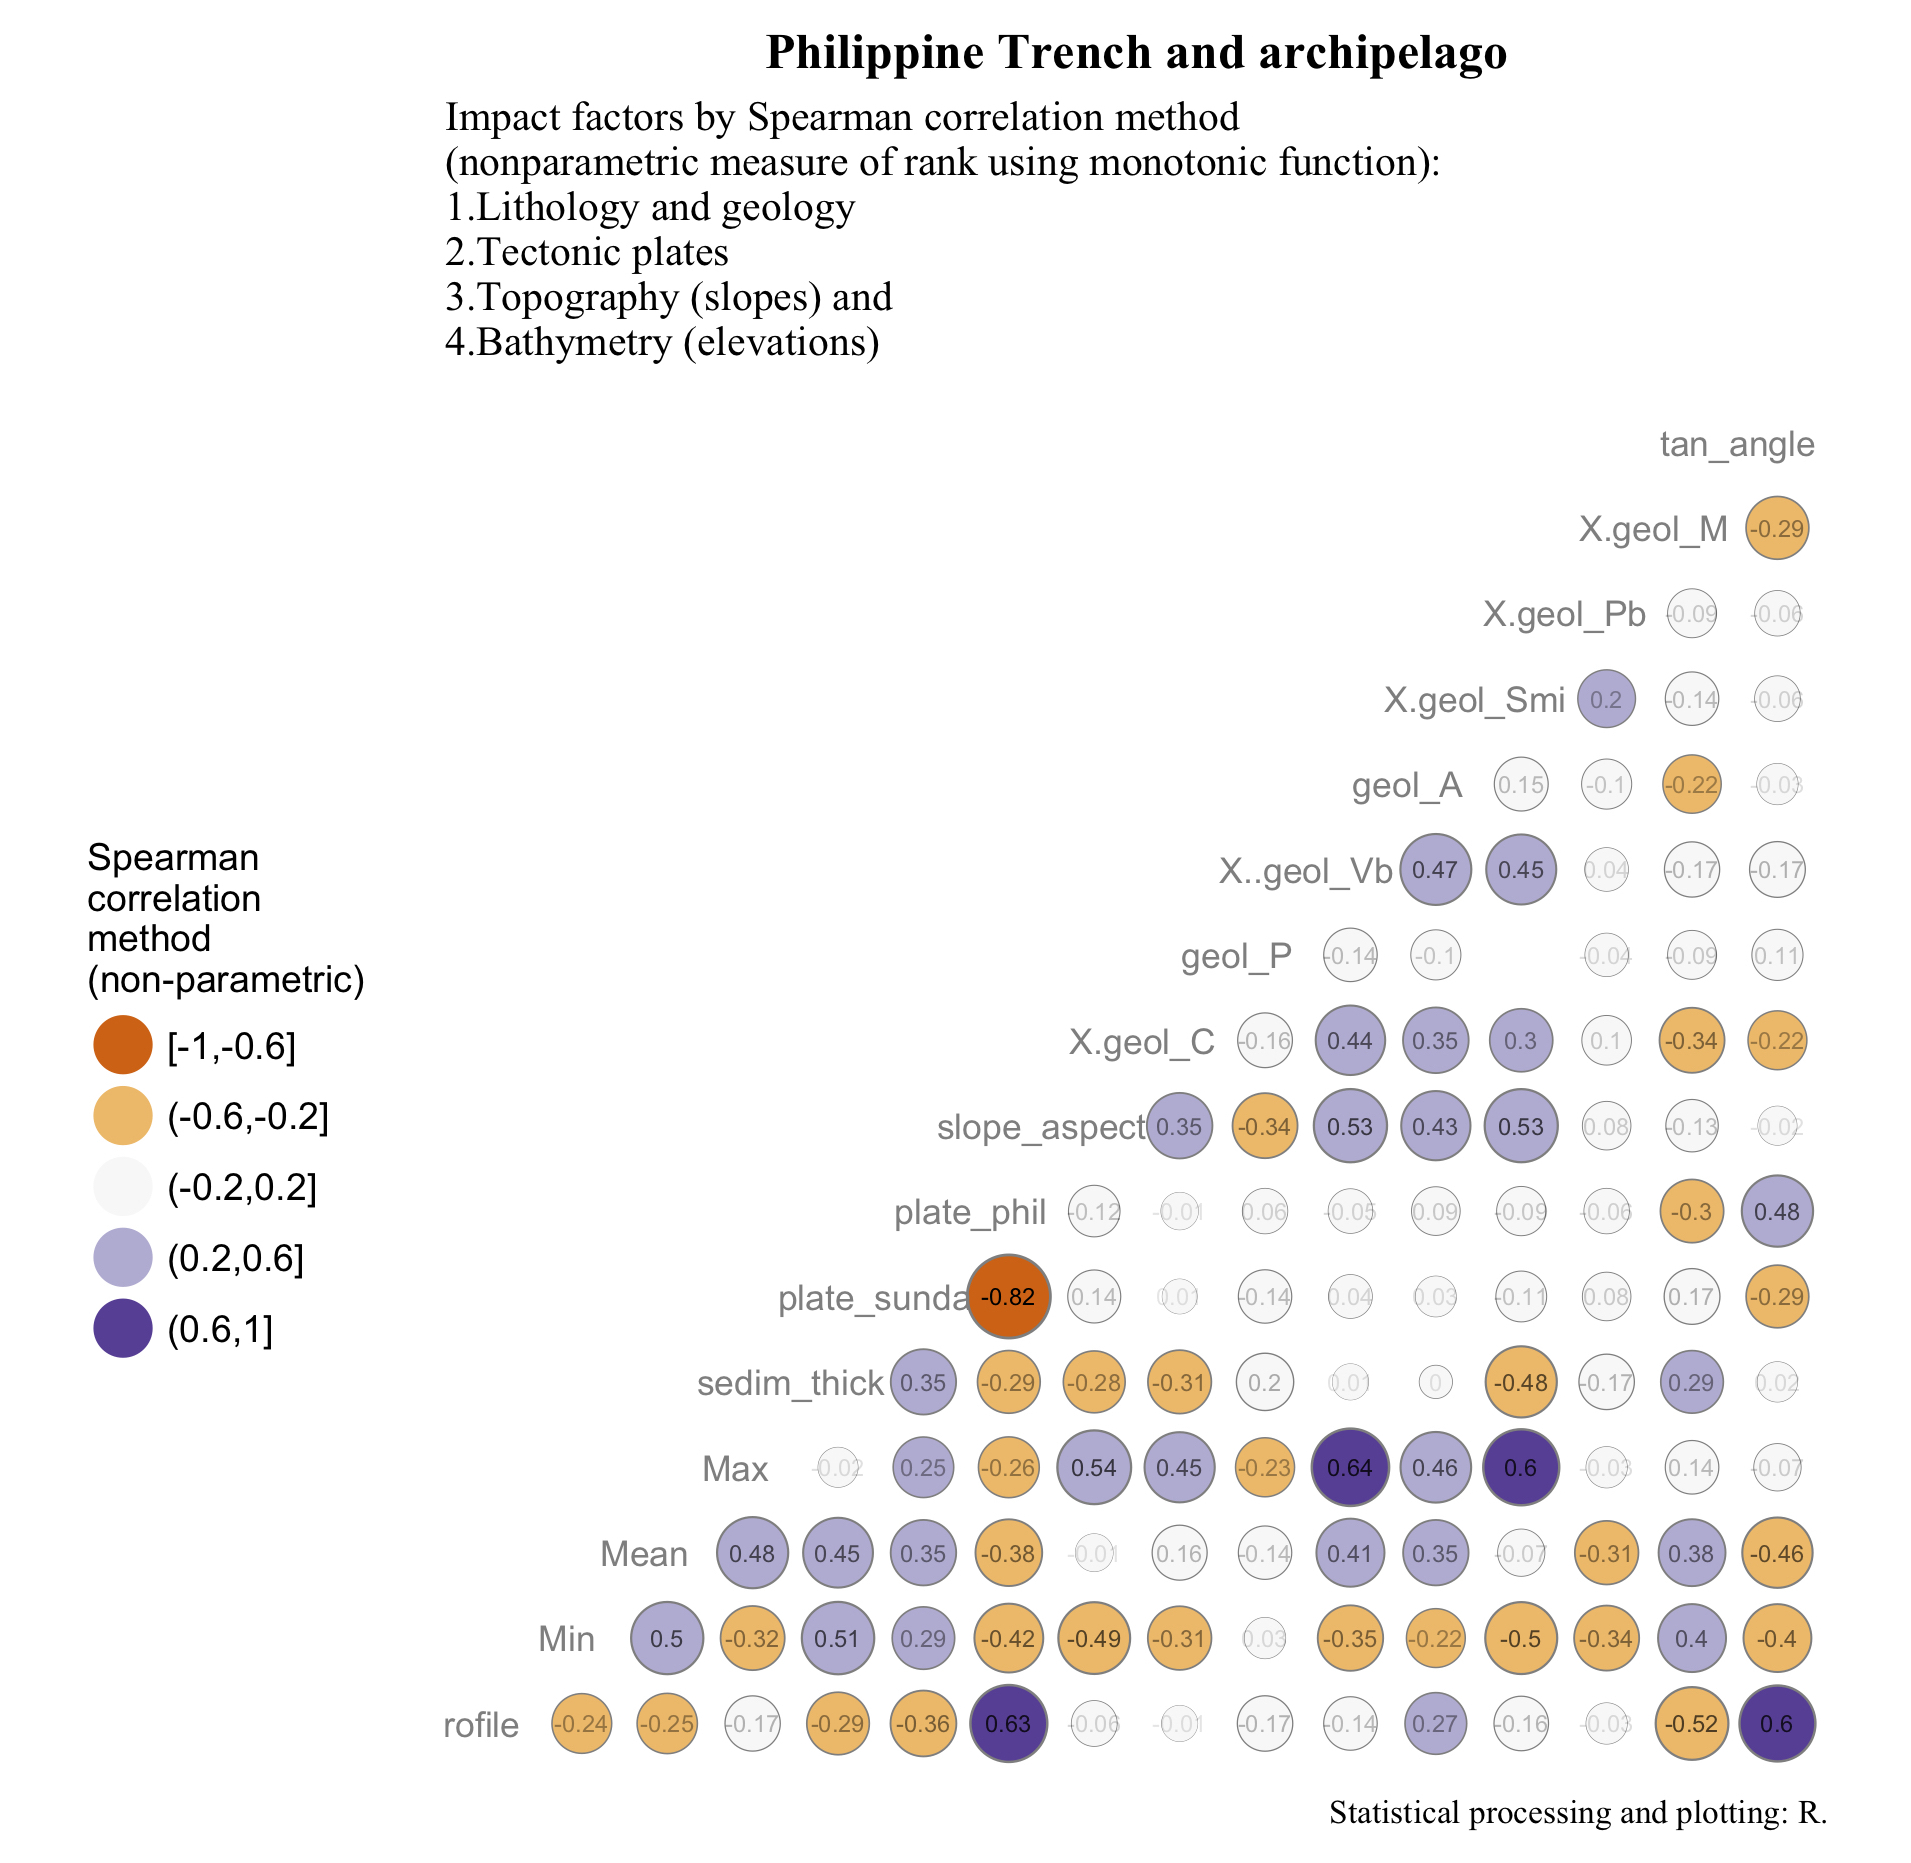
\includegraphics[width=10cm]{Fig-GML9.jpg}
	\caption{Correlation matrix by Spearman method visualizing influence of the impact factors on the geomorphology of the cross-section profiles. Plotting: R.}\label{fig:GML9}
\end{figure}

The fitted model of the matrix shows (Fig. \ref{fig:GML9}) following variables representing the relationships between the elements of the Philippine Trench system: elevation values as topographic and bathymetric sampling points (maximal, minimal and mean values of the depths and heights in meters), sediment thickness (in meters), number of observation samples across two tectonic plates (Sunda Plate and Philippine Plate), geomorphic elements of slope across the trench (tangent degree and slope aspect), and seven types of the geology (rock lithology: see Table 1 for details). The absolute coordinates were excluded as a factor to remove the effect of the geodetic location. In total 15 variables were tested using following attribute classes: geology: 7, geomorphology: 2, sedimentation: 1, tectonics: 2 and bathymetry: 3. The computed matrix is shown on Fig. \ref{fig:GML9}.\\
The effects of the variations in the slope degree were tested by computed tangent angles for each of the 25 profiles, respectively (Fig. \ref{fig:GML10} plot 1)  and repeated the analysis by ranking bathymetric profiles according to the geomorphic slope steepness (Fig. \ref{fig:GML10} plot 2). Finally, the grouping of the profiles by slopes was performed by dividing the range into five classes, as follows: ‘strong slope’, ‘very strong slope’, ‘steep slope’, ‘very steep slope’, ‘extreme slope’. 
		
\begin{figure}[H]
	\centering
	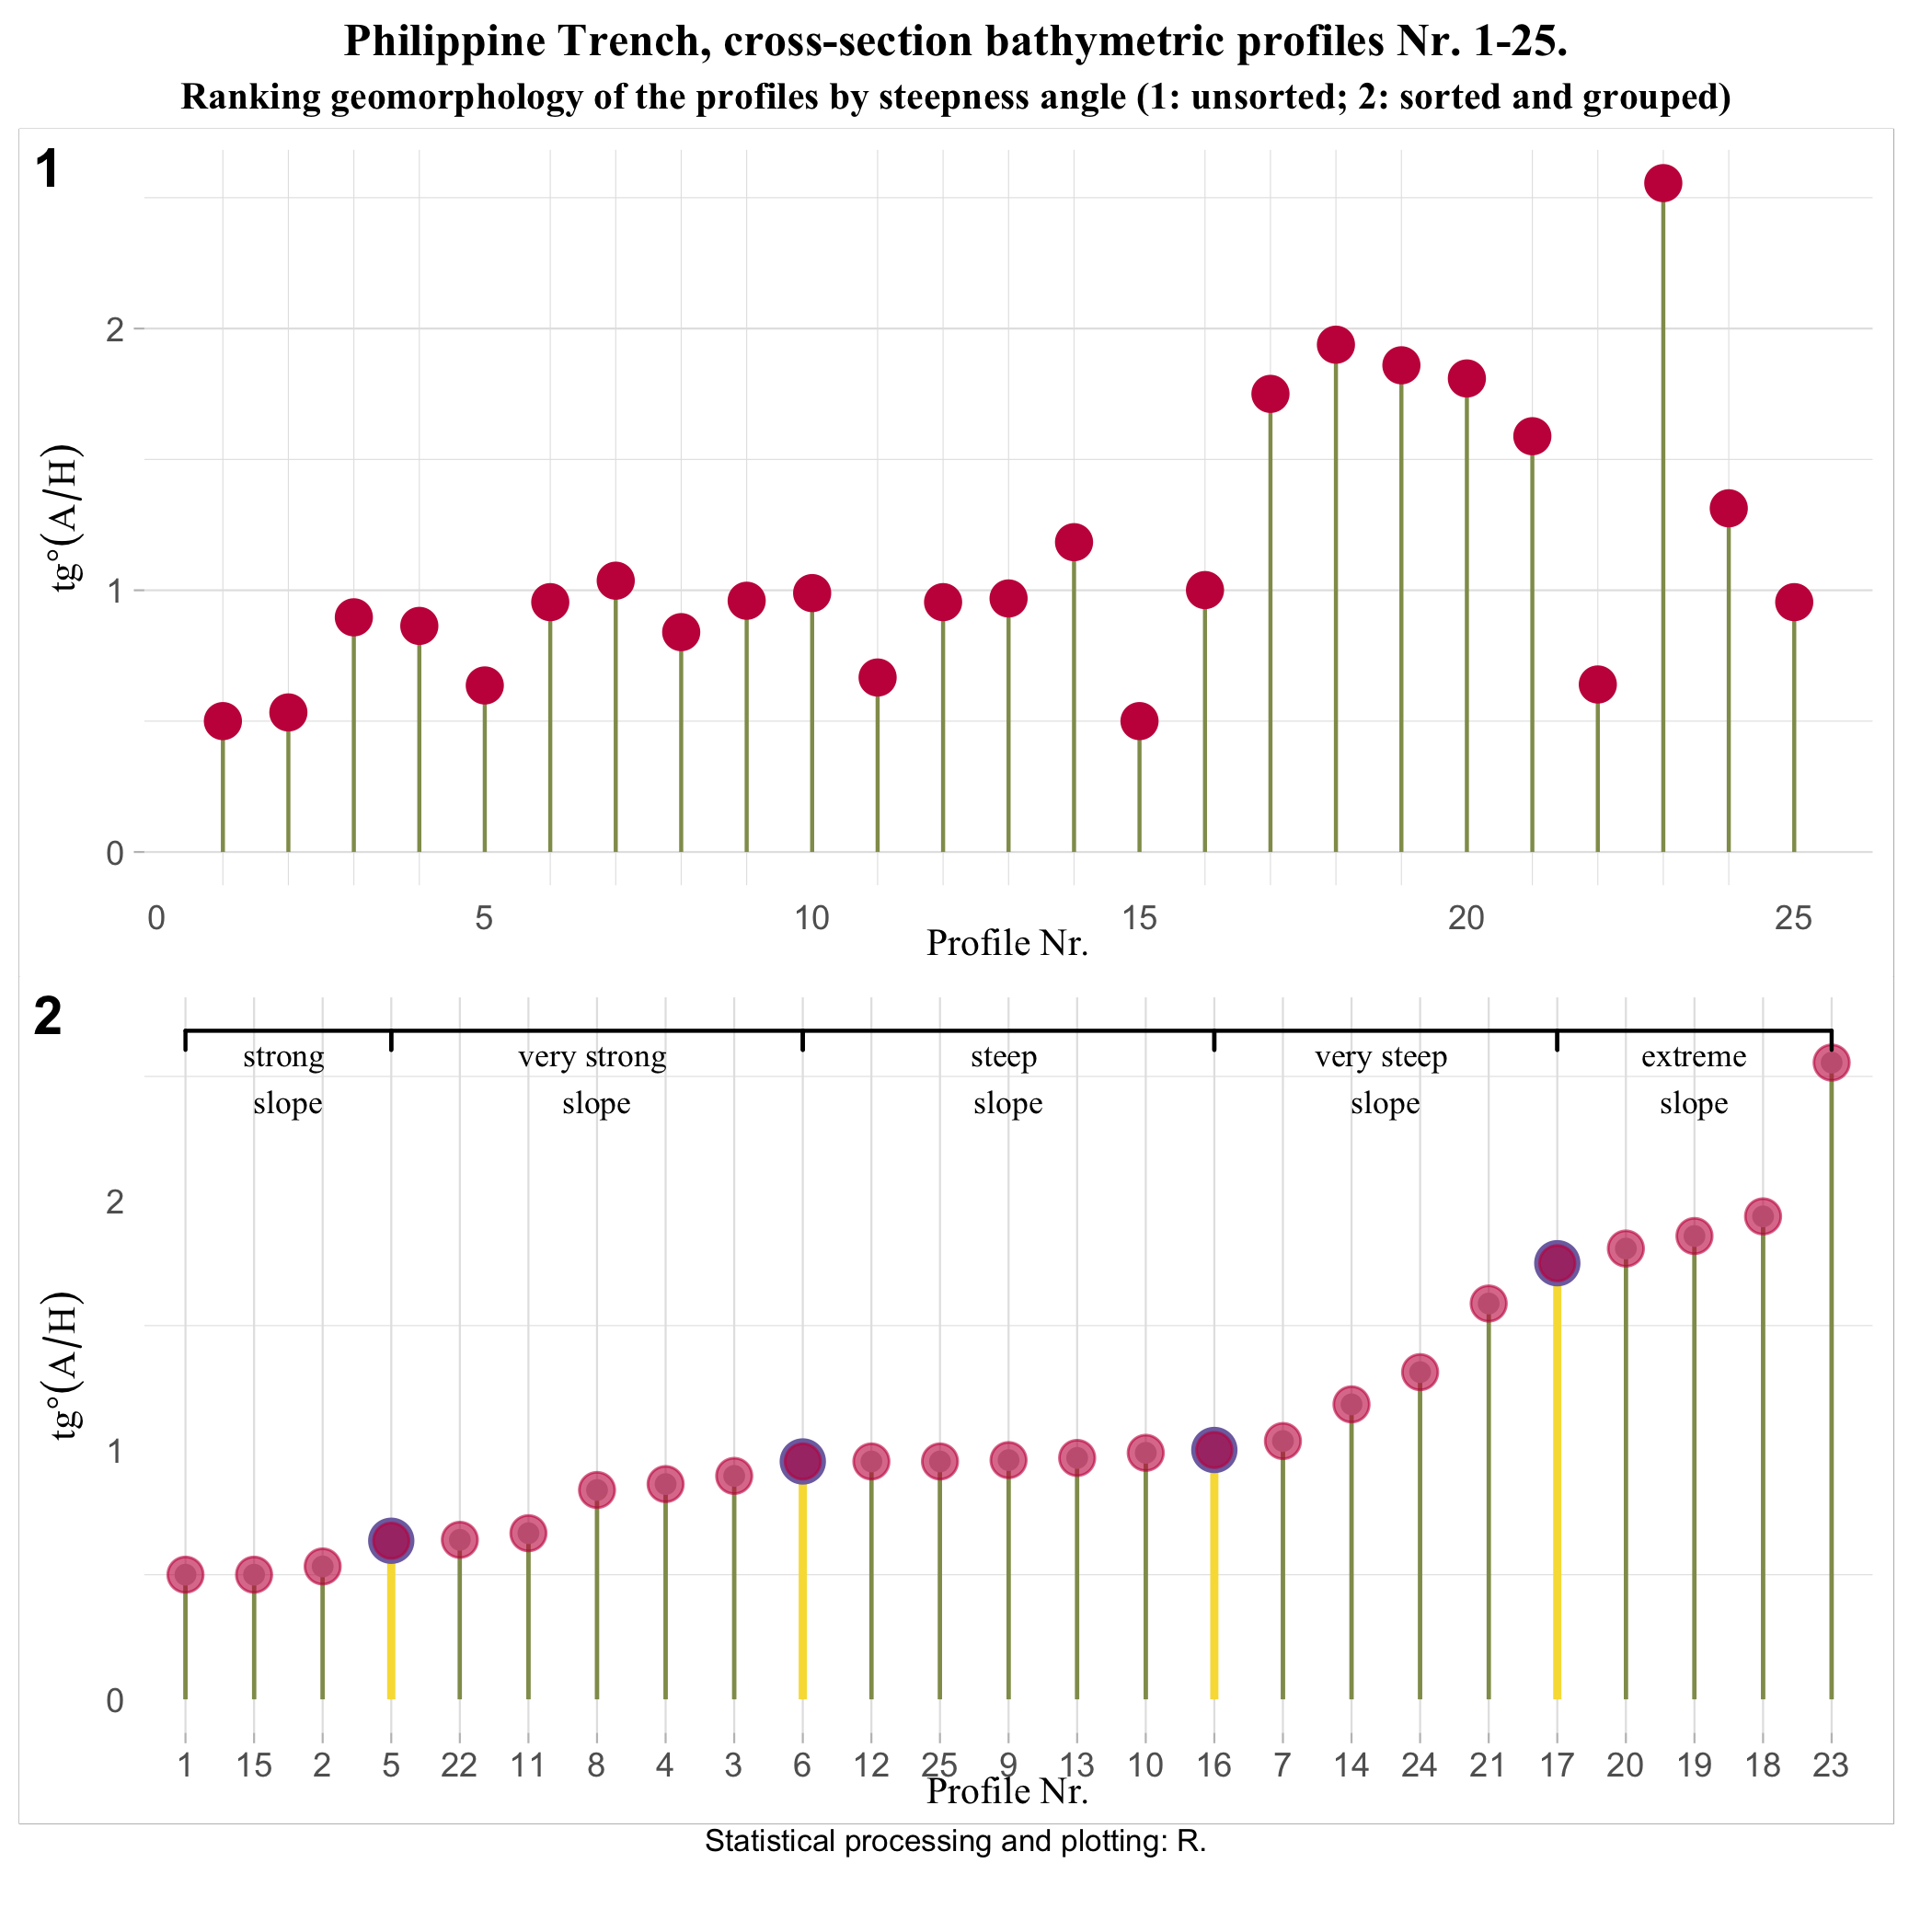
\includegraphics[width=10cm]{Fig-GML10.jpg}
	\caption{Ranking geomorphology of the cross-section profiles. Plotting: R.}\label{fig:GML10}
\end{figure}

The results presented in the data analysis on the Philippine Trench demonstrate the effectiveness of the data analysis in the marine geology. Using advanced data processing in Python it is possible to analyze various impact factors affecting the trench, understand the variability of the submarine geomorphology. Usage of the advanced methods of the statistical analysis enables to visualize combined effects of multiple geological and lithological attributes and factors that affect geomorphology of the hadal trenches. The results highlight the geomorphic variation and complex characteristics of the impact factors of geological origin affecting the Philippine trench. Location of the trench on various tectonic plates along with geological factors (sediment thickness) and lithology contributes in geomorphic shaping of the actual form of the Philippine Trench.  

\section{Manila Trench}

The results of the geomorphological modelling and mapping of the Manila Trench (Fig. \ref{fig:M6a}) shown spatial variation in the different parts of the trench. Two different trench segments were analyzed aimed at detecting their spatial changes for an area covering Manila Trench and adjusting Luzon Island \index[places]{Luzon Island} (northern Philippines \index[places]{Philippines}). The south-east directed second segment (plotted as green line on the Fig. \ref{fig:M6b}) shown steeper slopes on the oceanward side of the trench and deeper bathymetric records. On the contrary, northern segment (plotted as almost vertical yellow-colored line on Fig. \ref{fig:M6b}) demonstrated softer geomorphic shapes yet steeper gradient from the Luzon Island side. The fine-resolution data such as \ac{SRTM} grid was used to map bathymetry and topography of the study area and 1- min resolution from the gravity data (Jason-1, CryoSat).

\begin{figure}[H]
	\centering
		\includegraphics[width=10cm]{Fig-M6a.jpg}
	\caption{Transect of the cross-section profiles digitized along the of the Manila Trench}\label{fig:M6a}
\end{figure}

\begin{figure}[H]
	\centering
		\includegraphics[width=10cm]{Fig-M6b.jpg}
	\caption{Two segments of the cross-section profiles digitized along the of the Manila Trench}\label{fig:M6b}
\end{figure}

The statistical results (Fig. \ref{fig:M7}) show differences in the depth ranges of the Manila hadal trench along the Luzon island. The depth and geomorphology of the slope vary significantly for the depths range -3,500 to -4,500: minimal values are notable for the northern part of the trench where 526 observation points (18,2\%) are recorded for the depths -4,000 to -4,200 m, as shown on Fig. \ref{fig:M7} A. 

\begin{figure}[H]
	\centering
		\includegraphics[width=10cm]{Fig-M7.jpg}
	\caption{Histograms of the bathymetry of the Manila Trench}\label{fig:M7}
\end{figure}

The histogram for the northern part has a clear bimodal distribution with two peaks. The second peak shows areas crossing the Luzon island. On the contrary, southern part demonstrates 142 values for the minimal bathymetry with values -3,500 to - 3400 m; the second peak also shows areas of the Luzon Island. The comparison of the statistical data analysis clearly shows that the northern part of the trench is deeper.
\begin{figure}[H]
	\centering
		\includegraphics[width=13cm]{Fig-M8.jpg}
	\caption{Gradient trend modelling for the cross-section profiles of the Manila Trench}\label{fig:M8}
\end{figure}
The southern part of the trench has steeper slope gradient from the oceanward part and on the contrary, the northern part is steeper in the continental slope part (Fig. \ref{fig:M8}, A and F). The submarine terraces can be noted on the northern segment of the trench (Fig. \ref{fig:M8} F) at depths - 2,000 m. Generally, the modelling of the northern part shows more steep degree of the oceanward slope (pairwise comparing on Figure 8: subplots C and H; D and I; E and J).\\
However, a gradually slanting terrace on the southern part of the trench can be seen on the fragment 50-100 of the cross-section with depths from -1,100 to -1,300 m. Hence, the comparison between two segments of the trench located on the northern and south-eastern part of the trench show that northern part of the trench has shallower values of depths comparing to the southern yet more steep slope on the Luzon Island side.\\
As for the geophysical modelling, based on the patterns of the free-air gravity map of the Manila Trench (Fig. \ref{fig:M4}), the high density materials are distributed continuously from the northern the southern Taiwan vertically southwards to the Luzon Island \index[places]{Luzon Island}, the Philippines \index[places]{Philippines}  from -50 mGal to -200 mGal. The majority of the values in the South China Sea areas lie between the 10 to 30 mGal, while values reaching >60 mGal can be noted in the island areas and southern Philippines. The results of the geomorphological modelling and mapping of the Manila Trench highlighted underlying tectonics conditions where the collision of two tectonic plates causes instability in the region: often earthquakes, submarine volcanism, seismicity in this region.

\section{Ryukyu Trench}
The statistical results (Fig. \ref{fig:R8}) on the modelling Ryukyu Trench \index[places]{Ryukyu Trench} show certain differences in the depth ranges of the Ryukyu Trench along the Ryukyu Arc \index[places]{Ryukyu Arc}. The depth and geometry of the slope vary considerably: maximal values of -5,500 to -5,700 m are notable for the northern part of the trench where 334 observation points are recorded, as shown on Fig. \ref{fig:R8} (A). With a minor difference, southern part demonstrates comparable values (329 samples) for the same depth range.

\begin{figure}[H]
	\centering
		\includegraphics[width=10cm]{Fig-R6.jpg}
	\caption{Automatic digitizing cross profiles of the Ryukyu trench, green and yellow for southern and northern segments}\label{fig:R6}
\end{figure}

However, more significant differences can be seen for the depths >6,000 m. Thus, the southern part of the trench (shown on Fig. \ref{fig:R8} (B) has only few values (9 samples) with depths >6,800m while the northern part shows 41, 59 and 23 records, with a maximal values reaching -7,460 m. Moderate to shallow depths with ranges from -3,000 to -5,000 m are comparable for both parts of the trench with values not exceeding 68 samples for the northern part and 42 samples for the southern, respectively. \\
The forearc basin deeper than 2,000 m and shallower than 1,000 m \ac{BSL} shows more samples data in the northern part of the trench than in the south. In contrast, a wide terrace with depths shallower than 25 m is generally larger (161 samples) in the southern part of the trench. To conclude, the comparison between the two spatially different segments of the trench show that northern part of the trench has deeper depths comparing to the southern. This can also be noted on the Fig. \ref{fig:R1} where the deepest values of the central part are clearly seen with the deepest area extending seaward offshore from the Miyako Fault \index[places]{Miyako Fault} (Fig. \ref{fig:R2}).

\begin{figure}[H]
	\centering
		\includegraphics[width=13cm]{Fig-R7.jpg}
	\caption{Modelling of the trend curves showing general geomorphological transects and slope gradients using various mathematical approximations, GMT.}\label{fig:R7}
\end{figure}

As can be noticed on the comparison of Fig. \ref{fig:R6} A and Fig. \ref{fig:R6} B, the median stacked profile on the southern part (Fig. \ref{fig:R6} A) demonstrates slightly more gentle slope shape with submarine terraces, while there are no clear on northern part of the forearc slope (Fig. \ref{fig:R6} B). At the same time the depth of the forearc slope increases in the northern segment of the trench (Fig. \ref{fig:R6} B). These changes of the slope geomorphology are also highlighted by the contour of the increased marine free-air gravity anomaly, as a triangle shaped ‘island’ located at 126\degree E 24\degree N (Fig. \ref{fig:R4}). The geometric approximation of the trend curves (Fig. \ref{fig:R7}) shows similarity between the segments while applying coarse linear model (Fig. \ref{fig:R7}: E and J; Fig. \ref{fig:R7}: D and I). However, the differences in the geomorphic variations become more notable at the polynomial functions (Fig. \ref{fig:R7}: C and H; Fig. \ref{fig:R7}: B and G).

\begin{figure}[H]
	\centering
		\includegraphics[width=13cm]{Fig-R8.jpg}
	\caption{Statistical histograms showing frequency of the distribution of various depths values in southern and northern parts of the Ryukyu Trench.}\label{fig:R8}
\end{figure}

The geoid model shows geoidal undulation in the south-western part of the area east off Taiwan Island \index[places]{Taiwan Island} (Fig. \ref{fig:R3}). Generally, the major part of the area has geoid values range of 25 to 35 mGal. The increased values (>35 to 85 mGal) can be seen on the south-eastern part in the Philippine Sea area, while lower values (15-25 mGal) bordering continental shelf stretch along the East China Sea and the lowest (<15 m Gal) mainly occupy land areas.

\section{Palau Trench}

\section{Yap Trench}

\section{Mariana Trench}

Results on geomorphic modelling of the Mariana Trench profiles revealed that the major depth observation points of the Mariana Trench are located in between the -3000 and -5000 meters (Fig. \ref{fig:3-1-2}). 

\begin{figure}[H]
	\centering
		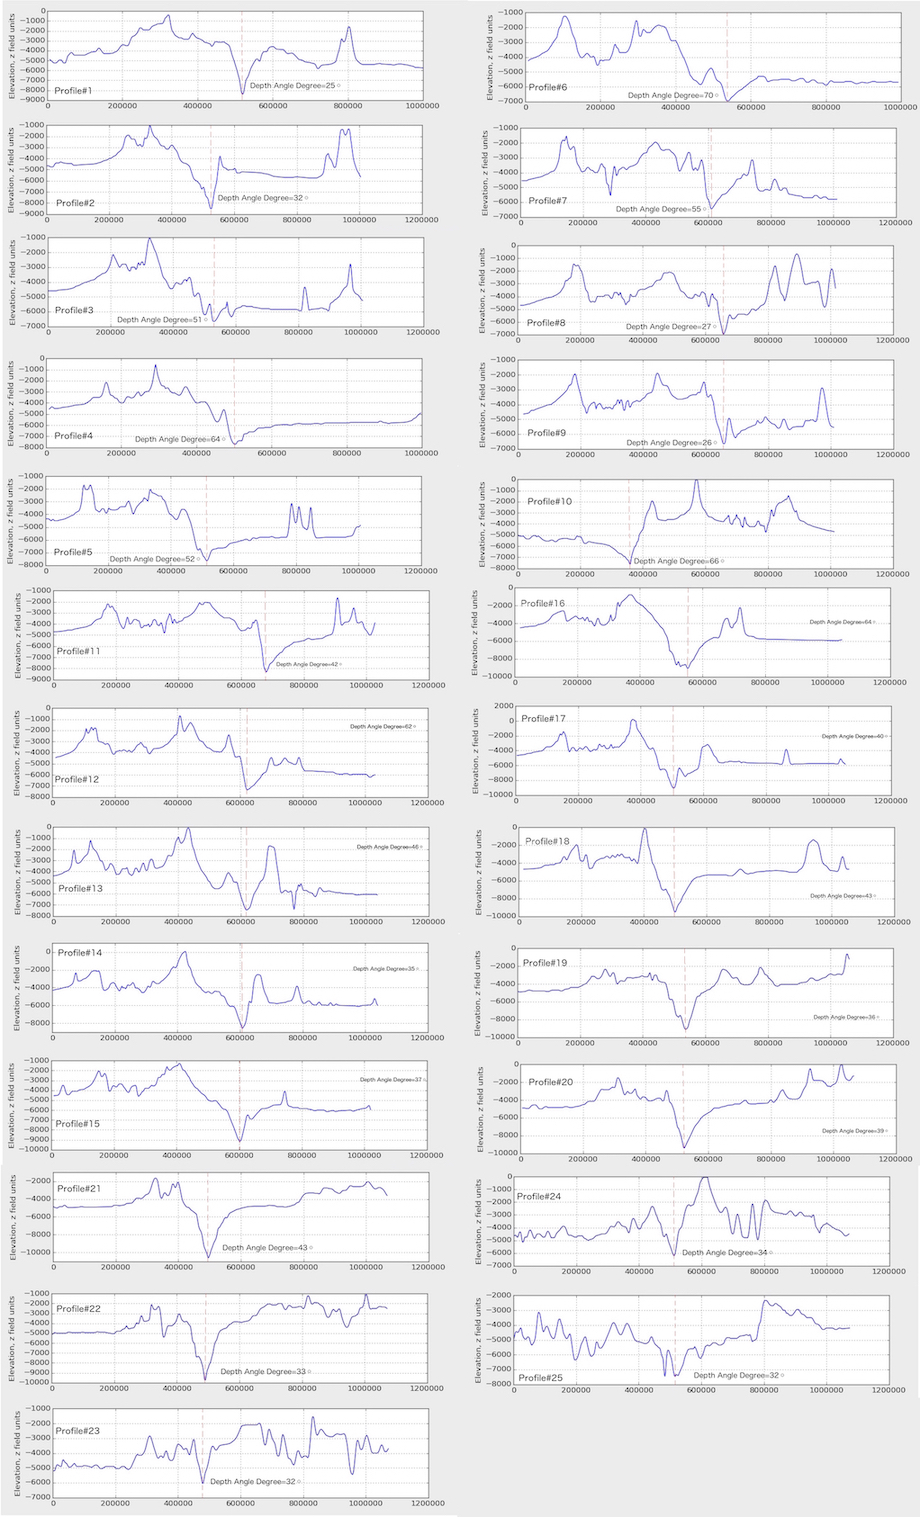
\includegraphics[width=12cm]{Fig-3-1-2.jpg}
	\caption{Graphs of the 25 bathymetric profiles, Mariana Trench, Quantum GIS 3.0}\label{fig:3-1-2}
\end{figure}

On the contrary, the maximal depths reach up to -10000 in the current dataset, as can be drawn from the Figure 11: profiles 20, 21, 22 crossing mostly Philippine tectonic plate (Figure 11). Another significant change is the decrease of depth in profiles 23, 24, 25, crossing Caroline tectonic plate, which may explain, among other factors the depth changes. Profiles Nr. 23 and 24 demonstrate the deepest depth data range. The created profiles are visualized on Figure \ref{fig:3-1-2}. Conversely, bathymetric profiles from 1 to 16 have gradual decrease in absolute depths (Figure 9), which can be noted in outliers sample location. A slight increase in absolute depths of the profiles nr. 4-8 was also observed of the Figure 8. \\
The majority of the observation points of the mentioned above profiles crosses the Pacific tectonic plate. The changes in bathymetry may, among others be explained due to the changed environmental factors of the underlying plate. Nevertheless, sedimental thickness changes notably both within the trench by profiles (1:25) and between four tectonic plates that Mariana Trench crosses: Philippine, Pacific, Mariana and Caroline. Since the tectonic properties and attribute values of them are not identical, the comparative analysis of how the data vary across four distinctive plates was performed. As can be seen on Fig. 9, right, the majority of the observation points are located in the Pacific and Philippine plate, following my Marian plate, while Caroline plate only covers a few points (red colored, Figure 11 left). The density distribution as shown on a combined plot (Figure 9) enables to compare the overlapping and maximal aptitude of the density curves both for the profiles and depth data distribution by four tectonic plates. Thus, the major trend of the trench angles located on the Pacific plate has downward general line trend. The Philippine tectonic plate, on the contrary, has a minimal peak by profiles \#14-21, and then moving upwards. The highest value for Caroline. Consequently, as can be drawn from the Figure 5, Mariana plate has the highest density of depth distribution values, followed by the Philippine plate, then Pacific and Caroline, respectively. \\
From two multiple panel by groups (Figure 7 and Figure 8) we can compare the slope angles and depth distribution by tectonic plates, respectively, one can see the unique patters of these categories by four plates. Summaries of the variations of the local polynomial regression of the bathymetric depths of the measured samples are presented on Figure 4. Upon a close examination of these summaries it can be observed that, with a mean depth value ranging from 5000 to of 3000 on the profiles, the widths of the confidence intervals are expanding more rapidly by the profiles 12 to 15 and 19 to 22 thus indicating on the large amplitude of the depths variations in this part of the Mariana Trench. The indication is that profile depth rather being affected by the local geographic conditions caused by the location on four different tectonic plates with varying environmental conditions. On the other hand, profiles 22 to 25 crossing Caroline tectonic plate (again refer to Figure 11, left), suggests that the absolute depth in this region change to become shallower than the profiles crossing Philippine and Pacific plates, and this phenomenon has adverse implications for deep inter-connections between these factors.

\subsection{Comparative Geospatial Analysis by Four Tectonic Plates}
Studies revealed that several environmental factors have distinct effect on the Mariana Trench morphology. Among them, findings indicate (Figure 10) that sediment sources at the Mariana Trench are connected with trench tectonics where the values of the sedimental thickness lie between 120 and 140, decreasing to 50 mm. Thus, sedimentation processes differ significantly by four tectonic plates (Mariana, Pacific, Philippine and Caroline), due to the overall complexity of the sediment environmental processes and trigger factors and mechanisms. Among other triggers and key factors for sedimental thickness are turbidity caused by gravity sliding, biochemical deposits, closeness of seismic zones, igneous volcanic areas and differences in the sedimentation mechanisms. Besides, due to the funnelling effect, trench sediment deposits speed is faster and therefore, thickness is greater than that of the abyssal basins.

\subsection{Findings in Correlation, k-means Clustering and Data Grouping}
The results of k-means algorithm show groups across all 25 profiles, with the number of groups represented by the variable. We tested several possible clusters from 2 to 7, and found out the optical number, that is 5: the cluster circle contained the optimal number of the observations and the overlapping was reasonably minimal (Figure 13 and Figure 14). The correlation matrix is presented on Fig. 16 showing crossing correlations in the combination of the environmental factors. Comparison of the bi-factor in-between the factors revealed pairwise correlation (Figure 17). Pairwise comparative analysis (Figure 17) enabled to observe a marked influence on the environmental variables as bi- factors. Thus, in response to the decreasing sedimental thickness the slope angle goes in parallel; location of the volcanic igneous areas cause a cyclic repetition of the curve for the slope angles, as well as those of igneous volcanic areas have certain correlation between the slope angle and aspect degree. Therefore, according to the findings, four environmental variable factors, namely slope angle, sedimental thickness, aspect degree and location of volcanic igneous areas, are affecting the geomorphological structure of the trench.	

\subsection{Findings in Data Partition and Ranking}
Analysis of the angle steepness of the cross-section profiles along Mariana Trench revealed (Figure 19) that a bunch of bathymetric cross-section profiles form cluster groups with similar geomorphic properties divided into five groups over the study area. Thus, profiles: 21, 22, 18 and 20 have all 'strong slope' tg\degree angle degree, which is an average of 0.05. Similarly, profiles: 15, 19, 16, 17, 14 and 2, belonging to class 'very strong slope', have an tg\degree angle of 0.057 to 0.058 (Figure 19). When compared with third group in the study area, such as class 'extreme slope' (profiles: 1, 11, 4, 5, 10 and 13), the average slope tg\degree angle fluctuating from 0.060 to 0.070. The forth group is class “steep slope” (profiles: 25, 12, 6, 8 3) with a slope tg\degree angle values from 0.070 to 0.075. Finally, the last group is notable for the highest steepness (profiles: 9, 7, 23, 24), with average slope tg\degree angle degree up to 0.079. Although the slope steepness is generally related to the slab subduction in this particular area, the nature of the slope expansion in the study area may also be associated with other factors such as topography, igneous closeness of the volcanic areas, and location (Pacific, Philippine, Mariana and Caroline plates). The data grouping has been created using libraries (tidyverse) and (ggsignif) for reordering and normalization of the steepness angle (Figure \ref{fig:4-3-17}). 

\begin{figure}[H]
	\centering
		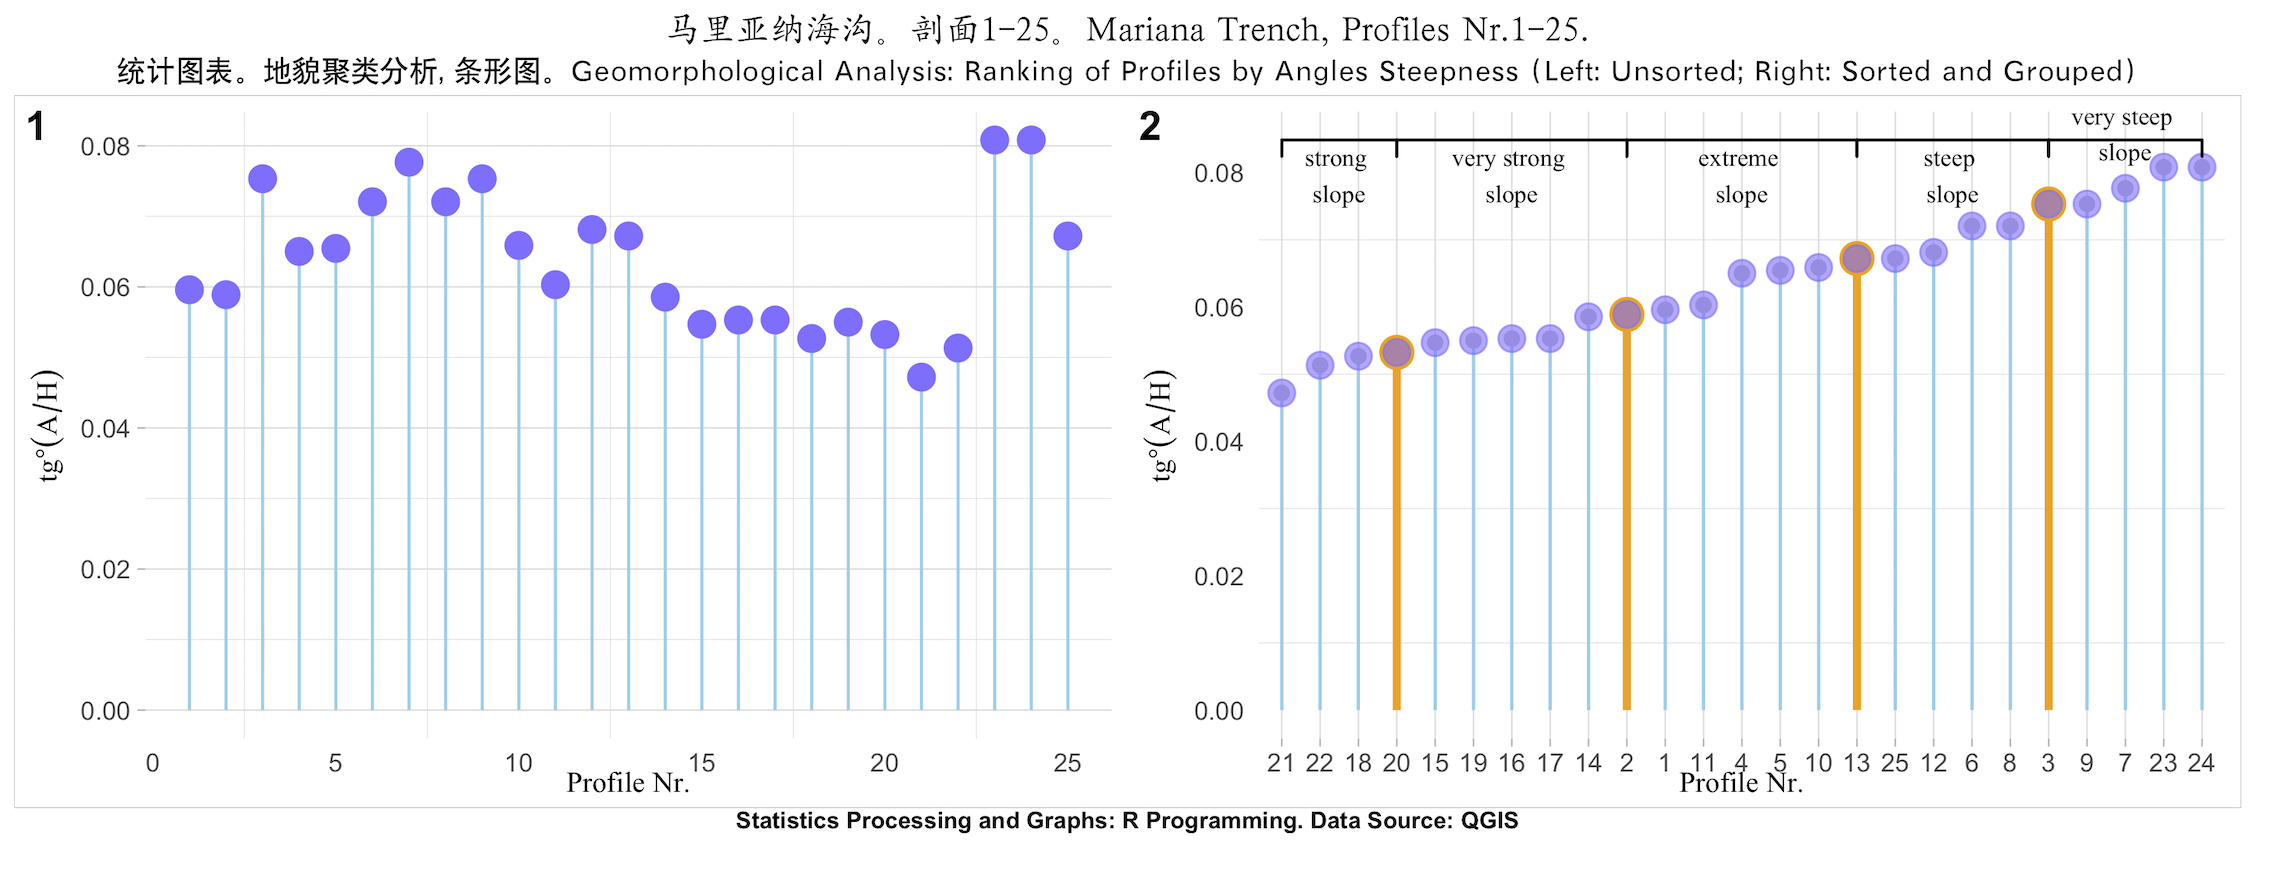
\includegraphics[width=13cm]{Fig-4-3-17.jpg}
	\caption{Steepness angles by the bathymetric profiles 1:25 of the Mariana Trench: unsorted (left); sorted and grouped (right). Computed and visualized in R: \ref{R:22}}\label{fig:4-3-17}
\end{figure}

In total 5 classes were created that include: strong slope, very strong slope, extreme slope, steep slope, very steep slope. They show classes of the steepness of the trench according to the results of the previously made cluster analysis and correlation matrix. 
Close examination of the slope degree statistical change revealed (Figure 18) that general trend has a scope of 0.03 (approximately from 0.05 to 0.08) of the steepness of the cross-section profiles along Mariana Trench. The re-classification of the slope angles across Mariana Trench (Figure 19, right), as well as statistical normalization have a crucial role in the analysis of the slope fluctuations. For instance, the profiles nr. 23 and 24 that are notable for the highest slope steepness, are location on the Philippine plate (Figure 11, right). Generally, two large classes of the normalized degree angles were observed (Figure 18): (1) below average degree (profiles nr. 1, 2, 11, 14-19, 21-22) and (2) below average degree (all the rest).\\
The spatial characteristics of the steepness distribution across trench have also been shaped by the components of the igneous volcanic areas in various profiles, as understood from Figure 22: profiles \# 20, 22, 23, 24 with notable amount of igneous volcanic observation points (over 180) correlate with steepness angle. As a result of close examination, the groups of five classes of the slope steepness within trench are selected as best suitable due to the changed geomorphic properties along the trench (Figure 22, right). Circular bar plots enabled to visualize depth distribution and slope angle values using R scripts are presented in \cite{Lemenkova201991}. \\

The Euler-Venn diagram enabled to analyze logical factors crossing and categories affecting morphology. It shows all possible logical relationships between a collection of data sets: four tectonic plates, sedimental thickness; geometric properties of the trench (that is slope angle, aspect class, hill shade group class derived as quantitative values from the GIS); morphology; volcanic closeness and depth values. As can be noticed (Fig. \ref{fig:4-3-10ab}) the area of the shape is proportional to the number of elements it contains, which is useful for explaining complex hierarchies and overlapping definitions as the case of factors affecting trench morphology. Mariana plate crosses all other plates, yet the most logical relationship has with Pacific plate. Comparing crossings between such categories as sedimental thickness and slope angle, as well as igneous zones distribution and trench slope angle. Thus, upon analysis of all possible combinations, intersections and similarities between categories, one can see the relationship between the mentioned above factors (Fig. \ref{fig:4-3-10ab}).

\subsection{Findings in Data Distribution: Kernel density curves}
	As can be drawn from the Figure 5, Mariana plate has the highest Kernel density of depth distribution values, followed by the Philippine plate, then Pacific and Caroline, respectively. Kernel density distribution has been shown in a combined plot enabling to compare the overlapping and maximal aptitude of the density curves both for the profiles and depth data distribution by four tectonic plates. The major trend of the trench angles located on the Pacific plate has downward general line trend. The Philippine tectonic plate, on the contrary, has a minimal peak by profiles \#14-21, and then moving upwards. The highest value for Caroline plate has profile \#23, while the maximal level for Mariana plate has profile \#7. The Philippine tectonic plate, on the contrary, has a minimal peak by profiles \#14-21, and then moving upwards. The highest value for Caroline plate has profile \#23, while the maximal level for Mariana plate has profile \#7.
	
\subsection{Findings in Composition charts}
	From the composition charts (Figure 8), drawn to compare the slope angles and aspect degree by bathymetric profiles, one can see the unique patters of these categories for the trench. The basic concepts of the close interrelation of various environmental factors (geological structure, bathymetric patters, tectonic plates location and subduction, spreading, transform fault, depths) affecting Mariana Trench formation is reflected in this paper. The technical tools consist of combination of R programming, GIS spatial analysis and mathematical algorithms for data processing and modelling. A comparison of the properties of the oceanic crust and ophiolite sections, sedimentary thickness and depth distribution across bathymetric profiles enabled to make a better understanding of the ties among geospatial factors influencing Mariana Trench formation. In turn, it facilitate a more reasonable forecast of the possible position of the mineral deposits fossils within Mariana Trench, for instance in the Philippine Sea tectonic plate.

\subsection{Impact factors affecting trench formation}
	Complex usage of programming tools, mathematical statistics and geospatial analysis enabled to get a differentiated understandings of the hadal environments of the Mariana Trench. The results revealed following three types of factors having the highest score: geometric (tg\degree slope angle), geologic (sedimental thickness) and tectonic structure. The results furthermore indicated that tectonic plates, sedimental thickness of the trench basement and igneous volcanic areas causing earthquakes play the most essential role in the geomorphology of the trench. \\
	Current studies reveled that there are factors influencing Mariana Trench geomorphic structure the most. The most affecting factors are as follows: sedimental thickness of the basement, slope angle steepness degree, angle aspect, bathymetric factors, such as depth at basement, means, median and minimal values, closeness of the igneous volcanic areas causing possible earthquakes, and geographic location across four tectonic plates: Mariana, Pacific Philippine and Caroline. Summary of the results is being represented on the Fig. 11 of \cite{Lemenkova201871} as a hierarchical tree map of impact factors generated using R code: \ref{R:38}.\\

Mariana Trench is important integral feature of the active continental margins of west Pacific Ocean. Mainland and oceanic sides of the trench have complicated steps of various shapes and sizes, caused by active tectonic and sedimental processes. The steepness of the trench depth averages in 4-5 \degree. Adjacent tectonic plates, however, have more steep angle with an average slopes of 10 to 15 \degree, but their individual parts can be limited to steeper slopes as subjects to the gravitational flow system of the submarine canyons and valleys. Complex distribution of the various geomorphic material on the adjacent abyssal plains of the ocean contributes to the formation of the geomorphic features of the particular region of the ocean bottom in Mariana Trench. It was furthermore found that slope degree and amplitude has important impact on the sedimental thickness, while the aspect \degree has lesser effect.
	
\subsection{Spatial variations in the trench morphology}
The geomorphological structure of the Mariana Trench has been impacted by various geological and geographic factors in response to the interconnected determinants of the system. Various studies have been undertaking to analyze the complexity of the system of deep ocean trenches and reveal possible impact factors (recent studies, e.g., \cite{Rijsingenvanetal2018}, \cite{Luoetal2017}, \cite{Yoshida2017}, \cite{Freymuthetal2015}, \cite{Ichinoetal2015}, \cite{CizkovaBina2015}, \cite{Boutelieretal2014}, \cite{Harrisetal2014}.

The studies of the ocean hadal trenches based on the profiles cross-section have been undertaken in the past (for instance, \cite{Murray1945}, yet based on the technical methods of that time. Until now, little attempts has been available on application of R programming language and scripting libraries towards studies of ocean trenches in marine geology. Deep ocean trench formation is a very complex process that is known to be influenced by a variety of geomorphological and oceanological factors. These may not adequately explain the process of trench deep formation, its further development and what is the impact in a variety of factors affecting hadal structure of the ocean trenches. An improvement of the technical tools is therefore required in such studies.\\
Current analysis of the Mariana Trench geomorphology and dependence of the variability of the angle steepness from affecting factors indicate that the importance of geological factors (closeness of the nearby igneous volcanic areas, location of the part os of the trench on certain tectonic plates, angle aspect and bathymetry, depth and sediment layer thickness) are highly variable. The complex tectonic and geomorphic features of the Mariana Trench has been reviewed using a set of tested 25 cross-section profiles with unique geologic conditions located in four tectonic plates that Mariana Trench crosses. The results of the data analysis on Mariana Trench demonstrated the dependences between the geomorphic factors and geology (slope angles and sedimental thickness, respectively) on the profile morphology. The quantified similarities between the distributional data distances were assessed using correlation matrices and cluster analysis (k-mean method).\\
The similarities and differences in the geomorphic structure (steepness of the slope angle degrees), geological characteristics (sediment thickness layer), geographic location of certain tectonic plates (Mariana, Caroline, Philippine and Pacific) and bathymetry (absolute minimal depths, means and median values) exist along the trench. Large gradients in variability occur within and among norther and southern part of the trench as well as in the eastern curve of its shape directed towards  transform lines near Magellan Seamounts \index[places]{Magellan Seamounts} and Marcus-Wake seamount \index[places]{Marcus-Wake Seamounts}. Hence, it enable to identify that geomorphological structure of the trench is mainly dominated by the following factors: the most dominated is geological factors: the closeness of the submarine volcanic areas and location of Philippine and Mariana tectonic plates, whereas sediment thickness is mainly geomorphic dominated. Thus, as a result of the undertaken study, it has been found that the middle part of the Mariana Trench (profiles: 14 up to 17), with very strong slopes, have roughly equal proportions of sediment thickness layer, which indicates that spatial locations and distributions of the volcanic areas and slope angle of the ocean trench are closely interrelated and affect sediment thickness. In addition to the variation of the slope degree, the variations in the sediment thickness by profiles were defined as indirectly impacted from the changed slope degree that gives conditions for the sediment accumulations. \\
The information and conceptual framework for the sediment thickness of the World Ocean published by \cite{Divins2003} was used in this research. Ranking geologic data has a step in geomorphic analysis where the levels of the slope degree are determined by the geospatial impact. Therefore, geomorphic variations typically necessitate an additional sub-task of the geological analysis of the study area. For example, if a certain segment of the trench is located near the active volcanic area the sedimentation rates may increase significantly in this particular region. For example, the profiles Nr. 1, 24, 25, 23 are notable for high sediment thickness on the Philippine Plate, profiles Nr. 2, 4, 6, 8 have the highest values for the Mariana Trench,  profiles Nr. 3, 5, 8, 6 have the highest values of the sediment thickness for the Pacific Plate, etc. The profiles located on the Caroline plate have the least values, since this part of the trench has only a few bathymetric points from the sample pool that cross the Caroline Plate. The results of the data analysis demonstrated spatial geomorphic unevenness of the Mariana Trench. Five unique regions across the trench length have been revealed, and the impact of various environmental factors affecting they morphology and characteristics were assessed by means of the applied statistics.

\section{Izu-Bonin Trench}

\section{Japan Trench}

\vspace{0.5em}
\begin{tikzpicture}[thick]
	\draw[decorate,Tan1,decoration={coil,segment length=5pt}] (0,4) -- (15,4); 
\end{tikzpicture}

\pagebreak

%%%%%%%%%%%%%%%% Chapter 5: Discussion %%%%%%%%%%%%%%%%%%

\chapter{Discussion}\label{chp:5}
	\markright{Discussion}

\section{Historical development of the ocean geomorphology}

	The history of the studies of ocean geomorphology, origin of the formation and types of the submarine landforms have been constantly arising interest of the geoscientists throughout the \nth{20} century until now, the chronology of the landmark research include, for instance: \cite{Daly1936}; \cite{Heezen1959}; \cite{Shepard1963}; \cite{HeezenTharp1977}; \cite{Agapovaetal1979}; \cite{Kennett1982}; \cite{Gorini2009}; \cite{Beckeretal2009}. Understanding a variety of factors that impact the geomorphology of the sea floor is a very complex task that includes a variety of the multi-disciplinary approaches that is geospatial data visualization, geostatistical analysis, geological modelling, etc. Rapid recent development of the IT technologies in \nth{21} century enables to analyze geological and oceanological stream data in large quantities which facilitates the studies of the marine geomorphology.\\  
	Mapping seafloor geomorphic features and understanding the factors of its variability centers several important components of the development of the marine geology. First,  support spatial marine observations and ecosystem management; second, supporting environmental monitoring of the marine areas; third, generating knowledge of the Earth’s shape; fourth, economic monitoring and evaluation of the seabed natural marine resources that has a strategic aim of governmental planning. Many attempt of the seafloor mapping and monitoring exist so far \cite{Carronetal2013}; \cite{IHOIOC2012}; \cite{Lanieretal2007}; \cite{NormarkCarlson2003} and the advances in marine seafloor mapping are constantly developing. \\ 
	The XX century is notable for the systematic ocean exploration using \ac{RS} methods, \ac{QGIS} tools for data processing and a variety of machine learning tools for data post-processing and statistical analysis. and integration with further statistical analysis: the plugins installed for reading the coordinates, re-projecting the coordinate systems, layout visualization and attribute data conversion into xls and csv tables were efficient enough for this research. The overlapping in \ac{GIS} enables to map and visualize crossing various layers (tectonic plates, location of the volcanic igneous areas), as well as reading coordinates and depth observation points. \\
	In XXI century, the advantages of the application of modern IT technologies for marine geology include, above all, the possibility to perform a scripting- and programming based approach for data analysis. A multi-disciplinary approach includes the \ac{GIS} geospatial analysis, algorithms of the data analysis provided by the high-level programming languages, such as Python and R. Combination of the advanced methods of scripting libraries together with spatial analysis by \ac{GIS} plugins and \ac{GMT} scripts enables to process marine geological data sets. Data in marine geology have specifically large volumes of the sampling observation points derived from the cruises. That is along with their variety and different types (e.g., lithology and rocks of the seafloor, geological structure, tectonics etc). Therefore, the velocity of the data processing by \ac{GMT}, reshaping tables in AWK, and statistical analysis supported by R and Python enable to operate with large data volumes, to generate new data frames for the reprocessing and modelling, which is indisputably actual for the oceanography. Given these reasons, the advantages of using programming in the ocean research opens clear and distinct perspectives. In addition, specifically designed libraries of Python and R embedded specialized techniques to extract the insights in the complexity of the marine geological factors affecting the structure of the submarine seafloor.
	
\section{Novelty}
There are both theoretical and practical innovations of the research presented in this dissertation that can be applied in the similar works. The theoretical novelty lies in the comparative geomorphological mapping of the two hadal trenches that does not exists in the available literature. The practical novelty consists in the developed methodology of the  cross-disciplinary approach that includes a sequence of the \ac{GMT} and IT tools (Python, R, Matlab, AWK) for data processing. The combination of the advanced tools of geospatial research (\ac{GMT} based \ac{GIS} project and data analysis on Python and R programming languages) enabled to perform complex statistical analysis based on the embedded mathematical algorithms. \\
As for cartographic approach, it should be stressed that a \ac{GMT}-based mapping was applied for the geospatial modelling instead of the traditional \ac{GIS}. Tested, presented and explained functionality of the several \ac{GMT} modules enabled to do automated digitizing of the orthogonal profiles crossing trenches in the perpendicular direction. Through this modelling, the shape of the landforms and steepness gradient of the trenches were visualized, compared and statistically analyzed. The traditional handmade cartographic digitizing is a tedious laborious routine usually prone to minor or major errors. On the contrary, using \ac{GMT} based machine learning for the automatization of the cartographic techniques significantly improves the quality and precision of the modelling.\\
Understanding structure of the submarine landforms of the hadal trenches as the deepest places on the Earth helps to improve investigations of the marine geology and submarine geomorphology of the oceans. Applying advanced spatial analysis for the the data analysis, processing and modeling, using advanced cartographic modelling tools enables to make deep insights in to the least accessible part of the Earth: the deep-sea trenches. \\
The research presented successful application of the scripting libraries of \ac{GMT} in marine geology which resulted in high quality precise mapping, fine cartographic instrument ray, flexibility of the scripting and coding, applicability of the UNIX utilities. Using such advantages of the \ac{GMT} for the geospatial data modelling and mapping definitely facilitates geodata processing, enables high precision analysis and mapping oceanographic data sets. As demonstrated in this paper, the application of the \ac{GMT} cartographic workflow towards geoinformation tasks, geological data analysis and visualization is highly effective and promising comparing to the traditionally used \ac{GMT} software.\\
Correct cartographic visualization is the key step towards proper understanding and detecting environmental factors in complex systems, such as geology, bathymetry, oceanography, tectonics. Therefore, precise mapping demonstrated by means of the GMT as proved in this paper is strongly recommended for further application on marine geological studies, especially for the geospatial analysis of the structure and functional features of the geospatial objects such as hadal ocean trenches. Advanced cartographic possibilities presented by the \ac{GMT} toolset results in high quality mapping by various techniques: diverse projections, color palette tables, location of the directional roses, selecting correct fonts and grid lines, illumination of the grids, etc. the results represented as a series of the thematic layers showing geological and geophysical phenomena of the study area. \\
Current work contributed both towards marine geological studies and towards technical demonstration of the advanced cartographic solutions in the GMT scripting workflow. High precision cartography, machine learning techniques and flexibility of the scripting ensure the high standards of the GMT and its suitability for the geospatial modelling. Main tasks demonstrated in this research included developed technical scripting methodology of the GMT modules for the data analysis. These included machine learning, digitizing cross-section profiles, visualizing and analysis of the data sets (gravity and topography surface modelling), 3D-mesh modelling, contour plotting, descriptive statistical analysis. \\
Analysis of the geospatial data by the GMT enables to map such remotely located areas as deep-sea trench with a given example of the \ac{MAT} and to analyze geophysical and geological factors of the study area. The GMT scripting toolset demonstrated effectiveness and functionality for the geospatial data analysis, precise and accurate cartographic mapping. Technical application of the advanced cartographic solutions and high quality mapping provided by the GMT scripting workflow demonstrated geoinformation data processing. The GMT script listings of the core research steps used to perform data analysis, oceanographic mapping and graphical visualization are presented. The proposed techniques and methodology of the GMT scripting presented in key processes of the workflow stepwise provided effective framework for the geological mapping and and can be applied for further geological tasks in similar research.

\section{Actuality}
The structure of the ocean seafloor has been the subject of the attention in Earth sciences recently \cite{Micallef}; \cite{Mitchell}. The rapidly developing GIS methods, machine learning algorithms and automatization in geospatial analysis improves the precision and quality of the mapping. One of these tools, the \ac{GMT}, a geospatial scripting toolset developed by \cite{WesselSmith1991} provides advanced cartographic solutions that enable to model, analyze, map, visualize and calculate the phenomena of the submarine geology that can only be studied by the \ac{RS} methods and complex algorithms of data analysis. A variety of the \ac{GMT} modules \cite{Wesseletal2013} specifically adjusted for modelling raster grids, plotting vector maps, computing descriptive statistical graphs and aesthetic cartographic mapping proved to be a perfect tool for modelling oceanological data. Due to its inaccessible location, the seafloor of the deep-sea trench can only be visualized using \ac{RS} tools and advanced algorithms of data analysis. The importance of the developing and technical improving of the innovative methods in cartographic data processing is indisputable. Automatization in data analysis has been significantly increased over the past years. However, using programming and scripting in cartography still remains lower comparing to the use of the traditional \ac{GIS}. \\
In view of the above said, the actuality of the current dissertation, fully based on using advanced data analysis (\ac{GMT}, Python, AWK, Matlab and R), is clear. The performed comparative analysis and geomorphic modelling of the hadal trenches located in the Pacific Ocean has a great scientific and practical interest. The first relates to the testing theory of plate tectonics. The second is caused by the estimation of the time and place of where earthquakes and tsunami may arise. Moreover, a correlation with distribution of the volcanic igneous areas, as well as economic needs for the mineral resources are other important goals for deep trench studies. The aim of the presented research was to identify bathymetric cross section profiles of the hadal trenches that show similarity by their complex parameters, so that they could be grouped into patters. \\
Using a sequence combination of the advanced data analysis (R, Python, AWK and Octave/Matlab programming, \ac{GMT} and \LaTeX visualization, \ac{QGIS} data processing), supported by the sound literature review, this study enabled to identify variabilities among the geomorphology of the major 16 trenches of the Pacific Ocean. The high accuracy of the performed statistical data analysis and cartographic supported by the chosen methodology of the machine data processing and algorithms as well as the high-resolution input data: raster grids, \ac{ASCII} xyzzy data, vector QGIS layers and attribute tables. They all were used for the data modelling and producing maps as a research output.

\section{Reflections on submarine geomorphology}
The question of the formation and structure of the ocean trenches has long attracted science. A variety of research has been done in various aspects of the trenches: bathymetric measurements, to assessment of volumes of mineral resources in the abyss, analysis of the pelagic and biotic communities, predicting earthquakes location and frequencies. Nowadays, sound statistical methods are elaborated as important additions for traditional \ac{GIS} methods of geospatial analysis of the deep ocean trenches. Without machine learning algorithms, a geospatial analysis of the big data cannot be considered as accurate and may lead to minor or major shortcomings and errors. machine learning is therefore indispensable for such remotely located areas as abyssal depths.\\ 
The bathymetry of the ocean floor reflects processes of the plate tectonics: movement, deformation and bending which is associated with mantle convection at the global scale. There are multiple factors influencing geomorphic structure of the hadal trenches the most: tectonic plates movement, sediment thickness of the basement, slope angle steepness degree, angle aspect, bathymetric factors, such as depth at basement, means, median and minimal values, closeness of the igneous volcanic areas causing possible earthquakes, and geographic location across the tectonic continental plates. The tectonic plates, sediment thickness and location of the igneous volcanic areas around the cross-section profiles play an essential role in the morphology of the trench. Complex distribution of various environmental factors on the adjacent abyssal plains of the ocean contributes to the formation of the geomorphic features of the ocean bottom in the trenches. Therefore, studying combination of these factors is a prerequisite for the correct understanding of the complex processes that take place in the abyssal environment of the hadal trench. \\
The geomorphology of the ocean hadal trenches reflects the fluvial geometry of the rivers, albeit in a rather general approximation. Setting aside the complexity of the real river structure that includes the mainstreams, branches and other geomorphic features \cite{Rosgen1994}; \cite{Stricketal2018}; \cite{Theiling1998} the overall approach of the riverine geomorphology may be adopted to the studies of the submarine canyon to come extent, in scope of the computer modeling and numerical analysis. The submarine canyons are important spaces within the ocean ecosystems \cite{DeLeoetal2010}. They may be approximated to the tributary river flows as channels for the flow of turbidity currents across the seafloor. The fine-grained sediments, e.g. clay and silt, are deposited from the turbidity currents channeled from the continental margins along submarine canyons down into deep ocean trenches. 
Hence, the interconnectivity between various parts of the ocean submarine geomorphology is very complex which requires a numerical approach in studies. Solutions proposed by the advanced data processing demonstrated in this research prove to be effective tool for the analysis of the data sets in marine geology.\\
Various factors affect formation, functioning and sustainability of the marine habitats and hadal trenches as one of the unique places of the oceans, as discussed in previous papers \cite{Pollnacetal2001}, \cite{Pelletier}. The complex analysis of the structure of the ocean ecosystem based on the advanced data analysis, software and scripting tools significantly increases the precision and speed of the data processing and reliability of the results. There are proven correlations between various geodetic features, bathymetric locations of the ocean trenches, geomorphic shapes and geophysical properties of the submarine phenomena (for example, \cite{MckenzieBowin1976}; \cite{SandwellSmith2009}; \cite{JimenezDiazetal2014}; \cite{JudgeMcNutt1991}; \cite{KalninsWatts2009}). Understanding the deep interconnections between various part of the ocean ecosystem gives a key to the proper modelling of the location of the ocean mineral resources and prognosis of the dynamic processes, e.g. earthquakes, tsunami. 

\section{Perspectives of the IT tools for geology}

Advanced data computing and processing by a combined approach of the advanced scripting tools for data analysis (\ac{GMT}, Python, R, Matlab, AWK) in marine geology is a promising dynamically developing extension of the existing traditional GIS tools. Scripting libraries and programming languages enable to deal with the massive amounts of the oceanographic data produced by cruise observations. That means, the batch processing of the big data becomes possible. Applying methods derived from the \ac{IT} and computer science domain and statistics towards traditional geological analysis increases the reliability of the results and the precision of the output. The number of use cases in processing large data sets in the marine geology is increasing since they are produced in a machine-generated stream in almost every oceanographic cruise as massive of the observation series taken from the research vessels, not only as a data arrays, but also as captured streams of video and imageries. \\
The value of big data in geoscience is indisputable nowadays. However, the question is not about the need for the massive data processing and their storage but in \emph{how} can we manipulate effectively with the large structured data sets in oceanography, and which \ac{ML} algorithms and advanced methods can be applied for the stream data processing. The effective answer to these questions are successively given by the programming languages, such as Python, AWK, Matlab and R that enable to process data arrays by complex methods. Graph-based analysis of the geological data modelling by GMT, Python, R and Matlab, together with table reshaping by AWK enables to process data as a stream through scripting, as demonstrated in this dissertation. \\
Effective data processing naturally helps to gain more insights into the seafloor geomorphology, dynamics of the tectonic slab processes, functioning of the marine ecosystems and benthos, directions of the water currents, and other parameters, otherwise not feasible by the traditional methods and approaches. Hence, current research demonstrated a multi-disciplinary approach combining effective manipulating of the spatial data sets by programming languages and scripting tools using statistical algorithms.	\\
The study demonstrated that the combined use of Python, AWK, R and Octave/Matlab programming is effective tool for the geospatial data processing. The study of the ocean floor is possible not only through the \ac{QGIS}, yet also by means of the available R statistical approaches: network analysis, factors analysis, plotting, diagrams, cluster analysis by various methods (k-means, dendrograms, silhouettes), triple correlation by ternary diagrams, to mention a few.\\
The paper presents an application of the R language towards geological studies with a specific case of the 16 deep-sea trenches of the Pacific Ocean. The sketch on the structure of the main factors of the hadal trench is presented, briefly summarizing tectonic plates movements, geological structure, sedimental conditions, bathymetry, lithological properties and other features of the trench system in the Pacific Ocean. It furthermore reviews the impact of the determinants on the trenches formation and structure, for instance, the relationship of the transform faults with rift valleys, location of the large igneous polygons. The methodology chapter is focused on the technical approaches of the study of the trench morphology by means of R programming, statistical analysis and GIS. The techniques of the classification are presented, including key R programming scripts. The results chapter highlights the findings received by the application of the technical methods (R programming, statistical algorithms and GIS) with geological analysis of the trench seafloor. The graphical and cartographic materials presented in this research support results and findings. Current work demonstrated that combination of R language, statistical algorithms and QuantumGIS is a highly effective decision for geospatial research aimed at processing multi-dimensional geospatial data sets. \\
The big data are often used in the marine research, since they are taken from the cruise observations and measurements in in-situ conditions. Therefore, the advantages of the programming languages lies in its usage for marine sciences lie in its effectiveness and functionality when operating large data sets. The \ac{ML} tools are highly effective for processing arrays and tables containing data of thousands of observation. Python is an interpreted language that enables programs to be written compactly and readably splitting them into reusable modules \cite{Rossumatal2018} that in turn process and model big data sets. Simple and vectorized syntax structures of Python enable to write code concisely yet effectively resulting in fewer bugs comparing to the codes written on C++. Using \ac{NumPy} for processing tables in .csv format and arrays facilitate advanced mathematical operations on large numbers of data. The encapsulation, inheritance and polymorphism of Python are the main advantages while working with big data in marine science and processing large tables. Examples of the application of programming languages and statistical tools specifically for the oceanological data modelling were presented in previous publications: Python \cite{Yuetal2019}; \cite{Lemenkova201905}, \cite{Lemenkova201989}, R \cite{Lemenkova201904}; \cite{Lemenkova201901}, \ac{SPSS} \cite{Lemenkova201990}, Gretl \cite{Lemenkova201988}. Using \ac{GMT} advanced scripting toolset for the cartographic modelling increases automatization of the mapping routine. Therefore, \ac{GMT} is strongly recommended for the geospatial data analysis and thematic mapping.\\
The importance of the precision of the numerical computing in Earth sciences cannot be underestimated. Current dissertation contributed towards the development of the numerical approaches in the marine geology demonstrating the combined usage of \ac{GMT}, Python, AWK, R and Octave/Matlab. The use of the \ac{IT} approaches in Earth sciences proved to be an effective method for the marine geology where data has to be statistically processed and visualized. Clear syntax and semantics of Python minimizes the chance of conflicts caused by hard-to-find bugs in a code.\\
The statistical data analysis has been implemented using \ac{ML} algorithms. The seamless integration of the multi-dimensional data by the R and Python statistical packages enabled to perform marine geodata analysis and proper selection of the optimal algorithms to process the data features. The fully provided codes written on the programming language make this research easily repeatable and accessible for other scientists. The adoption of the open source programming rapidly replacing the commercial technologies, Python and R will soon become popular among the marine geologists. This research contributes towards the development of the technical implementation of the \ac{ML} algorithms for effective processing of the geodata. 	
	
\vspace{0.5em}
\hspace{8em}\pgfornament[color=LightSteelBlue,width=10cm]{86}

\pagebreak

%%%%%%%%%%%%%%%% Chapter 6: Conclusion %%%%%%%%%%%%%%%%%%

\chapter{Conclusion}\label{chp:6}
	\markright{Conclusion}

The GMT cross-section stacking methodology as performed in this research proved to be a successful means of visualizing and plotting geomorphological models applied for the submarine bathymetry by effectively minimizing the hand-made cartographic routine. Indeed using GMT enables to automatically digitize profiles, then to perform statistical analysis by plotting histograms and model trends for the general shape of the profiles using mathematical models of the lines approximation. Several GMT modules were tested and applied for the cartographic visualization of the marine free-air gravity, geoid, bathymetric mapping, geomorphic modelling and statistical data analysis. \\
The presented research work focused on the classification of the influencing environmental factors of three main groups (tectonics, bathymetry, geology) affecting formation of the Mariana Trench. The research is expected to lead to a significant improvement of our understanding of the relevant influencing geomorphic factors for the analysis of the ocean trenches. Additionally, the review of the correlation methods presented in the current research can be applied methodologically for comparing and benchmarking different research schemes on ocean trench analysis. Furthermore it can be used for analysis of submarine earthquake connections with ocean trench formation and tectonic slab movement or the controlling of impact factors during the geospatial analysis.\\
An application of R and Python programming languages for the geostatistical data processing with a case study of the Mariana Trench, Pacific Ocean. The formation of the Mariana Trench, the deepest among all hadal oceanic depth trenches, is caused by complex and diverse geomorphic factors affecting its development. Mariana Trench crosses four tectonic plates: Mariana, Caroline, Pacific and Philippine. The impact of the geographic location and geological factors on its geomorphology has been studied by methods of statistical analysis and data visualization using R and Python libraries. \\
The QGIS based methodology included following steps. Firstly, vector thematic data were processed in \ac{QGIS}: tectonics, bathymetry, geomorphology and geology. Secondly, the 25 cross-section profiles were drawn across the trench. The length of each profile is 1000-km. The attribute information has been derived from each profile and stored in a table containing coordinates, depths and thematic information. Finally, this table was processed by methods of the statistical analysis on R and Python. The programming codes and graphical results are presented. The results include geospatial comparative analysis and estimated effects of the data distribution by tectonic plates: slope angle, igneous volcanic areas and depths. 

\section{Global Summary}\label{sec:8}
	\markright{Global Summary}
The main innovative idea of this research was integrated usage of R and Python programming languages and statistical analysis towards marine geological studies. Geological studies of such complex geomorphic-oceanological system as Mariana Trench has specific points that distinguish it from the study of the valleys located on continents.\\
First, the rocks of the ocean floor are a closed object, which it is studied mainly by geophysical, i.e. remote, methods. These observations include the study of cores obtained from drilling vessels or platforms, samples collected while dredging the seabed.\\
Secondly, the knowledge of the geology of the ocean is connected with a thorough understanding of the basics of geophysics, geography, geomorphology, oceanography, cartography, informatics and principles of the data interpretation. Therefore, a complex variety of methods is necessary to study Mariana Trench that has been demonstrated in this research by R and Python programming languages.\\
Current research was intended to highlight the problem of the Mariana Trench very complex formation consisting of a variety of environmental factors. Mariana Trench is formed as an ocean seafloor geomorphological structure located in the zones of the continental margin tectonic plates bending. Moreover, a special attention was paid to the application of the algorithms of factor analysis: scripts with screen shots of codes, correlation matrix, as well as visualization of factor analysis. As a case study of this research, the application of R and Python programming towards geoscience studies successfully revealed impact factors affecting the abyssal morphology of the Mariana Trench. It contributed towards question of how we can measure and analyze the structure of trench in the least reachable location of the World Ocean.\\
The ocean conservation nowadays becomes one of the most vibrant, paramount endeavors of the marine ecology since due to the global circulation, even the remotely located areas are not exempt from the anthropogenic impact \cite{RichmondKotowicz2015}. Understanding the structure of the marine habitats at the deepest places of the hadal trenches helps to improve investigation of the marine biology communities of the ocean. Before now, the hadal trenches were thought to have restricted life activities, which is caused by the extreme environmental conditions. Those include high hydro-pressure, submarine volcanism related to tectonic plate subduction, as well as lack of ultra-violet and food supply. Nevertheless, recent research reports, \cite{Linleyetal2016}; \cite{Linleyetal2017} shown vast microbial and faunal community structure, abundance, biodiversity, level of endemism and adaptation towards extreme condition in hadal marine species. This created a special attention towards hadal biosphere where specific life conditions are created including geological, geomorphic, and biochemical factors {\cite{Liuetal2018b}}; \cite{Leducetal2016}; \cite{Joydasetal2018}. Moreover, deep-sea ecosystems recently arisen a considerable commercial interest due to their potential to serve a various range of the industrial needs \cite{Senetal2016}. Understanding such complex remotely located environments is crucial for the development of the marine biology. Using high-level programming languages and embedded algorithms for the statistical analysis of large data sets, which are almost always the case for the marine biology studies is a prerequisite for the precise data analysis and environmental forecasting. Current paper presented successful application of the Python and R languages towards oceanographic research with a case study of Mariana Trench. 

\section{Recommendations}\label{sec:9}
	\markright{Recommendations}
	
As a recommendation for further research focused on ocean trenches, a traditional methods of the seafloor studies at the GIS level should always include a set of statistical analysis tools such as R and Python, or alternatively, python (e.g. \ac{SciPy}, \ac{NumPy}, matplotlib), Matlab, Octave. Studies of the spacial data series are usually accompanied by the graphics in view of the facetted plots that can facilitate comparison of the data by groups. This is especially useful while collecting multi-dimensional various geophysical data. Since there are many deep interconnections among factors affecting the formation, morphology and development of the trench, mathematical algorithms and objective analyses based approaches are to be used to study marine geo-systems.\\
A contemporary perspective of \ac{GMT}, R and Python based geostatistical methods for the analysis of trench structure and formation is demonstrated in this research. The application of the statistical tools provided by functionality of R and Python programming offer optimal prospects for better understanding of the bathymetry of the deep ocean trenches with a case study of the ocean trenches. A rigorous and quantitative quantitative data analysis performed by R and Python and supported by \ac{GIS} geospatial analysis methods is effective tool for investigation of such complex and large-scale geologic structures as deep ocean trenches. This paper demonstrated an example of such cross-disciplinary quantitative approach for geomorphological analysis. Through example of the presented research the powerful tool of the R and Python scripting approach was shown. Using R and Python for marine geoscience research does not only make geological modelling simpler and less error-prone. It may also facilitate more complex simulations involving, for instance, multi-dimensional modelling runs with varying geological parameters. It is also possible to apply the developed methods for extending testing of other deep ocean trenches.\\
Recent advances in the understanding of the hadal structure of the Mariana Trench have, so far, relied on the technologies that were unable to analyze correlations between various factors affecting its functioning and morphology. As demonstrated in this research, active using functionality of the programming languages for geoscience research provides effective tools to improve approaches to study hadal bathymetry. Development in statistical methods and using R and Python scripting libraries in oceanographic studies make it possible to treat multi-source types of the marine geology data.\\
Full R and Python codes and workflow of the statistical methods outlined in the current paper enable their repeatability and reuse for further testing in similar research. Hence, current paper contributed towards technical development of the quantitative and statistical methods in marine geomorphologic and oceanographic studies, in particular those aimed at the objective analysis of the complex interplay between the factors affecting ocean trench geomorphology.\\
This thesis presented a view of the Python and R programming application towards modelling of the variations in the submarine geomorphology of the ocean trenches. A specific case study is set on the west Pacific Ocean, Mariana Trench. It described the methodological approaches and use of the selected statistical libraries aimed at geomorphic variation modelling with Python and R snippet of codes provided for repeatability.\\
Significant differences in the variation modelling in geomorphological research in marine geology can result from the application of various methods and algorithms, different approaches proposed by selected libraries of programming languages (R, Python or Octave) or used software (e.g., Gretl or SPSS), reported by various authors \cite{BilinaLawford2009}; \cite{Gill2001}. Therefore, the geomorphic modelling of depths is limited to the selected algorithms, applied approaches and available data sets. 
 
\section{Outlook and future developments}\label{sec:10} 
	\markright{Outlook and future developments}
	
A thorough multi-dimensional data processing in marine geology should include following data: tectonic (continental margin plates), geological (geologic structure), lithological (sedimentation) and oceanological (direction of the deep currents). Processing multi-source data by the \ac{ML} methods enables to speed up our understanding of the submarine geomorphology of the ocean seafloor. A combination of the advanced tools for spatial data processing, such as R, Python, AWK and Octave/Matlab programming, \ac{GMT}enables to perform integration of such complex heterogeneous data from a variety of sources for the in-depth analysis. \\
Future work should therefore consider applying other \ac{GMT} modules and their combination to develop complex approaches of the cartographic-geophysical investigations: earthquake intensity modelling, mapping detailed volcanic arcs, etc. Application of the \ac{GRASS GIS} is also recommended as a powerful GIS for the raster data processing. The combination and overlapping of various geospatial data as layers aimed to examining and quantifying geomorphological submarine landforms in connection with tectonic settings would enable to get more information of these data using advanced geospatial data analysis. Other recommendation for the future research could be integration of the \ac{GMT} with programming and advanced statistical packages that absent in \ac{GMT}: clustering, dendrogram plotting, factor analysis, \ac{PCA}.\\
From all the available statistical methods it is necessary to select the most suitable to the modelling type: data ranking, data distribution (e.g. box plots or ‘violin’ plots, linear regression or isotonic regression), correlation matrix or correlogram ellipses, etc. The correct chosen algorithm of the statistical modelling enable to best visualize and analyze the data set. Visualizing the full range of the geomorphology across the trench can be done using various methods: by the deepest values (i.e. each profiles can have only one dot point), or by showing the full line of profile (i.e. the profile shows the cross section in its length), in circular or bar plot or dot plot types, as presented in this paper. \\
In case the surface of the whole trench is being modeled, the extrapolation or interpolation of the depths by geomorphic profiles may lead to the possibility to increase random errors due to the complex nature of the real situation of physical environment. It can be either the effects of the external environmental factors over the geomorphic structure of the selected profile (e.g. tectonic slab movement that affects the shape of the trench segment) or mathematical approaches of the chosen algorithm of the approximation of the measured depths. In the most difficult parts of the trench (for instance, where trench crosses two or three tectonic plates), it is possible to intake more dense profiles digitizing. However, in this case it whole be reasonable to large scale this particular area of the selected study area as enlarged fragment.

\vspace{1em}
\pgfornament[height=1cm,color=Thistle]{77}
\pgfornament[height=1cm,color=Thistle,symmetry=v]{77}
\pgfornament[height=1cm,color=Thistle,symmetry=h]{77}
\pgfornament[height=1cm,color=Thistle,symmetry=c]{77}
\pgfornament[height=1cm,color=Thistle]{77}
\pgfornament[height=1cm,color=Thistle,symmetry=v]{77}
\pgfornament[height=1cm,color=Thistle,symmetry=h]{77}

\pagebreak

%%%%%%%%%%% Author's Publication %%%%
\begin{refsection}
\chapter*{Author's Publications}\label{chp:7}
	\addcontentsline{toc}{chapter}{Author's Publications}
	\markright{Author's Publications}
		\nocite{Lemenkova201992}
		\nocite{Lemenkova201991}
		\nocite{Lemenkova201990}
		\nocite{Lemenkova201989}
		\nocite{Lemenkova201988}
		\nocite{Lemenkova201905}		
		\nocite{Lemenkova201904}
		\nocite{Lemenkova201901}	
		\nocite{Lemenkova201871}			
		\nocite{Lemenkova201868}		
		\nocite{Lemenkova201866}		
	\printbibliography[heading=none]
\end{refsection}
\pagebreak

%%%%%%%%%%%%  Appendix  %%%%%%
\begin{appendices}
\pagenumbering{roman}
\appendix \label{app}
\appendixpage
	\counterwithin{figure}{section}
	\counterwithin{table}{section}
	
\chapter{Programming codes}\label{chp:8}

\section{Octave/Matlab language}
\subsection{Octave/Matlab script for cartographic visualization of the bathymetric profiles}\label{Oc:01}
\lstinputlisting[language=Octave]{Octave.m}

\section{\TeX \space macro language}
\subsection{\LaTeX code to create bathymetric profiles}\label{L:01}
\lstinputlisting[language=tex]{Latex-bathymetry.tex}
\pagebreak

\section{AWK language}
\subsection{AWK shell script for table reshaping}\label{Awk:01}
\lstinputlisting[language=awk]{AWK.sh}
\pagebreak

%%%%%%%%%%%%%%%%%%% GMT scripts start %%%%%%%%%%%%%%%%%%%%%%%
\section{GMT shell/bash scripts}
\subsection{GMT script for bathymetric mapping, ETOPO1 (here: KKT)}\label{GMT:01}
\lstinputlisting[language=bash]{GMT-01.sh}
\pagebreak

\subsection{GMT script for 3D mesh grid modelling, DEM based (here: AT)}\label{GMT:02}
\lstinputlisting[language=bash]{GMT-02.sh}
\pagebreak

\subsection{GMT script for bathymetry contour mapping (here: KKT)}\label{GMT:03}
\lstinputlisting[language=bash]{GMT-03.sh}
\pagebreak

\subsection{GMT script for geoid modelling (here: KKT)}\label{GMT:04}
\lstinputlisting[language=bash]{GMT-04.sh}

\subsection{GMT script for geological World map}\label{GMT:05}
\lstinputlisting[language=bash]{GMT-05.sh}
\pagebreak

\subsection{GMT script for regional geological map (here: MAT)}\label{GMT:06}
\lstinputlisting[language=bash]{GMT-06.sh}
\pagebreak

\subsection{GMT script for free-air gravity modelling (here: KKT)}\label{GMT:07}
\lstinputlisting[language=bash]{GMT-07.sh}
\pagebreak

\subsection{GMT script for generating and plotting stacked cross-sectioning bathymetric profiles (here: MAT). Profiles info: 400 km long, spaced 20 km, sampled every 2km}\label{GMT:08}
\lstinputlisting[language=bash]{GMT-08.sh}
\pagebreak

\subsection{GMT script for topographic surface modelling from the xyz ASCII data (here: MT)}\label{GMT:09}
\lstinputlisting[language=bash]{GMT-09.sh}
\pagebreak

\subsection{GMT script for gridding xyz data by Nearest Neighbor algorithm (here: KKT)}\label{GMT:10}
\lstinputlisting[language=bash]{GMT-10.sh}
\pagebreak

\subsection{GMT script for regression trend1d mixed models (here: AT)}\label{GMT:11}
\lstinputlisting[language=bash]{GMT-11.sh}
\pagebreak

\subsection{GMT script for 2D bar histogram and rose diagram (here: MAT)}\label{GMT:12}
\lstinputlisting[language=bash]{GMT-12.sh}
\pagebreak

\subsection{GMT script for 3D bar histogram plot (here: KKT)}\label{GMT:13}
\lstinputlisting[language=bash]{GMT-13.sh}
\pagebreak
%%%%%%%%%%%%%%%%%%% GMT scripts end %%%%%%%%%%%%%%%%%%%%%%

%%%%%%%%%%%%%%%%%%% Python scripts start %%%%%%%%%%%%%%%%%%%%%%%
\section{Python language scripts}

\subsection{Python code for statistical data analysis by violin plots}\label{P:01}
\lstinputlisting[language=python]{Python-01.py}

\subsection{Python code for clustermap: bathymetric data distribution by profiles}\label{P:02}
\lstinputlisting[language=python]{Python-02.py}

\subsection{Python code for histograms: distribution of the observation samples}\label{P:03}
\lstinputlisting[language=python]{Python-03.py}

\subsection{Letter-value plots for the Mariana Trench bathymetry}\label{P:04}
\lstinputlisting[language=python]{Python-04.py}
\pagebreak

\subsection{Python code for the strip plots (here: Philippine Trench)}\label{P:05}
\lstinputlisting[language=python]{Python-05.py}

\subsection{Python code for the correlogram matrices by Seaborn library}\label{P:06}
\lstinputlisting[language=python]{Python-06.py}

\subsection{Python code for the regression analysis}\label{P:07}	
\lstinputlisting[language=python]{Python-07.py}

\subsection{Python code for Letter-value plots for the Mariana Trench bathymetry}\label{P:08}	
\lstinputlisting[language=python]{Python-04.py}

\subsection{Python code for joint Hexagonal and KDE plots}\label{P:09}
\lstinputlisting[language=python]{Python-09.py}

\subsection{Python code for the correlogram plot (here: Pearson's method)}\label{P:10}
\lstinputlisting[language=python]{Python-10.py}

\subsection{Python code for a box-and-whisker plot for the Mariana Trench bathymetry}\label{P:11}
\lstinputlisting[language=python]{Python-11.py}

\subsection{Python code for sorting data in stem plots: analysis of the angle steepness}\label{P:12}
\lstinputlisting[language=python]{Python-12.py}

\subsection{Python code for plotting dendrograms}\label{P:13}	
\lstinputlisting[language=python]{Python-13.py}

\subsection{Python code for 3D scatter plots: correlation of the factors (sediment thickness, slope steepness, bathymetry)}\label{P:14}
\lstinputlisting[language=python]{Python-14.py}

\subsection{Python code for ANOVA}\label{P:15}
\lstinputlisting[language=python]{Python-15.py}

\subsection{Python code for \ac{KDE}, example for the subplot (F)}\label{P:16}
\lstinputlisting[language=python]{Python-16.py}

\subsection{Python code for stacked area charts on the bathymetry}\label{P:17}
\lstinputlisting[language=python]{Python-17.py}

\subsection{Python code for the facetted plot of the radar charts}\label{P:18}
\lstinputlisting[language=python]{Python-18.py}

\subsection{Python code for the distribution of the bathymetric data by stacked bar plots}\label{P:19}
\lstinputlisting[language=python]{Python-19.py}

\subsection{Python code for analysis of the distribution of sediment thickness, stacked bar charts }\label{P:20}
\lstinputlisting[language=python]{Python-20.py}

\subsection{Python code for pie charts visualizing bathymetry vs tectonic plates}\label{P:21}
\lstinputlisting[language=python]{Python-21.py}

\subsection{Python code for QQ plots visualizing descriptive statistics for the bathymetry}\label{P:22}
\lstinputlisting[language=python]{Python-22.py}

\subsection{Python code for WLS calculations}\label{P:23}
\lstinputlisting[language=python]{Python-23.py}

\subsection{Python code for quantile (QQ) regression}\label{P:24}
\lstinputlisting[language=python]{Python-24.py}

\subsection{Python code for SARIMA model}\label{P:25}
\lstinputlisting[language=python]{Python-25.py}

\subsection{Python code for Euler-Venn diagrams}\label{P:26}
\lstinputlisting[language=python]{Python-26.py}
%%%%%%%%%%%%%%%%%%% Python scripts end %%%%%%%%%%%%%%%%%%%%%%%

%%%%%%%%%%%%%%%%%%% R scripts start %%%%%%%%%%%%%%%%%%%%%%%
\section{R language scripts}
\subsection{R code to create histograms using (ggplot) library}\label{R:01}
Source data available on my \href{https://github.com/paulinelemenkova/R-1-Histograms}{GitHub}.
\lstinputlisting[language=R]{R-01.r}
\pagebreak

\subsection{R code to generate boxplots 'whiskerplots' using default boxplot function}\label{R:02}
Source data available on my \href{https://github.com/paulinelemenkova/R-2-Boxplot-Whiskerplot-}{GitHub}.
\lstinputlisting[language=R]{R-02.r}
\pagebreak

\subsection{R code for notched boxplot using (ggboxplot)}\label{R:03}
Source data available on my \href{https://github.com/paulinelemenkova/R-2-Boxplot-Whiskerplot-}{GitHub}.
\lstinputlisting[language=R]{R-03.r}

\subsection{R code to generate \ac{QQ} quantile statistics for facetted wrapped plot}\label{R:04}
Source data available on my \href{https://github.com/paulinelemenkova/R-3-QQ-Statistics-ECDF-Facet-Wrapped}{GitHub}.
\lstinputlisting[language=R]{R-04.r}

\subsection{R code for regression analysis for the bathymetric profiles}\label{R:05}
Source data available on my \href{https://github.com/paulinelemenkova/R-4-Regression-Analysis}{GitHub}.
\lstinputlisting[language=R]{R-05.r}

\subsection{R code for cluster analysis, dendrograms}\label{R:06}
Source data available on my \href{https://github.com/paulinelemenkova/R-5-Cluster-Analysis-Dendrogramms-}{GitHub}.
\lstinputlisting[language=R]{R-06.r}


\subsection{R code for correlogram by (ggplot) library}\label{R:07}
Source data available on my \href{https://github.com/paulinelemenkova/R-6-Correlogram}{GitHub}.
\lstinputlisting[language=R]{R-07.r}

\subsection{R code for Principal Component Analysis (PCA)}\label{R:08}
Source data available on my \href{https://github.com/paulinelemenkova/R-7-Principal-Component-Analysis-PCA-}{GitHub}.
\lstinputlisting[language=R]{R-08.r}
\pagebreak

\subsection{R code for k-means clustering}\label{R:09}
Source data available on my \href{https://github.com/paulinelemenkova/R-8-k-means-Cluster-Analysis}{GitHub}.
\lstinputlisting[language=R]{R-09.r}

\subsection{R code for Pairwise Standard Scatter Plots of k-means Cluster Correlation (comparing 4 tectonic plates)}\label{R:10}
Source data available on my \href{https://github.com/paulinelemenkova/R-8-k-means-Cluster-Analysis}{GitHub}.
\lstinputlisting[language=R]{R-10.r}
\pagebreak

\subsection{R code for 'lollipop' charts and diverging bars by (ggplot) library}\label{R:11}
Source data available on my \href{https://github.com/paulinelemenkova/R-9-10.-Lollipop-Charts-and-Diverging-Bars}{GitHub}.
\lstinputlisting[language=R]{R-11.r}
\pagebreak

\subsection{R code for Dumbbell chart by (ggalt) and (ggplot2) libraries}\label{R:12}
Source data available on my \href{https://github.com/paulinelemenkova/R-11-Dumbbell-Charts}{GitHub}.
\lstinputlisting[language=R]{R-12.r}
\pagebreak

\subsection{R code for categorywise bar charts}\label{R:13}
Source data available on my \href{https://github.com/paulinelemenkova/R-12-Categorywise-Bar-Chart}{GitHub}.
\lstinputlisting[language=R]{R-13.r}
\pagebreak

\subsection{R code for dot plot with encircling by (ggalt) library}\label{R:14}
Source data available on my \href{https://github.com/paulinelemenkova/R-13-Dotplot-with-Encircling}{GitHub}.
\lstinputlisting[language=R]{R-14.r}

\subsection{R code for double-Y axis using (LatticeExtra) library to perform comparative analysis of categories}\label{R:15}
Source data available on my \href{https://github.com/paulinelemenkova/R-14-Double-Y-Axis}{GitHub}.
\lstinputlisting[language=R]{R-15.r}

\subsection{R code for circular barplot by library tidyverse}\label{R:16}
Source data available on my \href{https://github.com/paulinelemenkova/R-15-Circular-Barplot}{GitHub}.
\lstinputlisting[language=R]{R-16.r}
\pagebreak

\subsection{R code for multiple strip plots divided groups, by LatticeExtra library}\label{R:17}
Source data available on my \href{https://github.com/paulinelemenkova/R-16_Strip-Plot-by-Groups}{GitHub}.
\lstinputlisting[language=R]{R-17.r}

\subsection{R code for multiple panels by groups (tectonic plates, depths, slope angles)}\label{R:18}
Source data available on my \href{https://github.com/paulinelemenkova/R-17-Multiple-panels-by-groups}{GitHub}.
\lstinputlisting[language=R]{R-18.r}

\subsection{R code for density curves: data distribution}\label{R:19}
Source data available on my \href{https://github.com/paulinelemenkova/R-18-Density_Curves}{GitHub}.
\lstinputlisting[language=R]{R-19.r}
\pagebreak

\subsection{R code to generate brackets for the specific regions along the Mariana Trench using library (pBrackets)}\label{R:20}
Source data available on my \href{https://github.com/paulinelemenkova/R-20-Scatterplot-with-overlapping-points-Brackets}{GitHub}.
\lstinputlisting[language=R]{R-20.r}
\pagebreak

\subsection{R code for radar chart using (fmsb) library}\label{R:21}
Source data available on my \href{https://github.com/paulinelemenkova/R-21-Radar-Chart}{GitHub}.
\lstinputlisting[language=R]{R-21.r}

\subsection{R code for highlighted group in lollipop chart by libraries (ggsignif) and (tidyverse)}\label{R:22}
Source data available on my \href{https://github.com/paulinelemenkova/22-R-Highlighted-Groups-in-Lollipop-Chart}{GitHub}.
\lstinputlisting[language=R]{R-22.r}

\subsection{R code for Euler-Venn Diagram (logical correlation of objects) using (venn) library}\label{R:23}
Source data available on my \href{https://github.com/paulinelemenkova/23-R-Euler-Venn_Diagram-Rose}{GitHub}.
\lstinputlisting[language=R]{R-23.r}
\pagebreak

\subsection{R code for animation using (gganimate), (gapminder) and (ggplot2) libraries: regression analysis plots for 25 bathymetric profiles}\label{R:24}
Source data available on my \href{https://github.com/paulinelemenkova/24-R-Animation}{GitHub}.
\lstinputlisting[language=R]{R-24.r}
\pagebreak

\subsection{R code for 'violin' plots using (violinmplot) library: statistical analysis of bathymetric data distribution}\label{R:25}
Source data available on my \href{https://github.com/paulinelemenkova/25-R-Violinplot}{GitHub}.
\lstinputlisting[language=R]{R-25.r}
\pagebreak

\subsection{R code for Exploratory Factor Analysis (EFA) using (FactoMiner), (factoextra) and (psych) libraries}\label{R:26}
Source data available on my \href{https://github.com/paulinelemenkova/26-R-Factor-Analysis}{GitHub}.
\lstinputlisting[language=R]{R-26.r}
\pagebreak

\subsection{R code for hexagonal plot by library(hexbin): bathymetric data distribution, Mariana Trench}\label{R:27}
Source data available on my \href{https://github.com/paulinelemenkova/27-R-Hexagonal-Hexbin-plot}{GitHub}.
\lstinputlisting[language=R]{R-27.r}
\pagebreak

\subsection{R code for \ac{ANOVA} for Mariana Trench}\label{R:28}
Source data available on my \href{https://github.com/paulinelemenkova/28-R-ANOVA}{GitHub}.
\lstinputlisting[language=R]{R-28.r}
\pagebreak

\subsection{R code for Ternary Diagram by (ggtern) library}\label{R:29}
Source data available on my \href{https://github.com/paulinelemenkova/29-R-Ternary}{GitHub}.
\lstinputlisting[language=R]{R-29.r}
\pagebreak

\subsection{R code for silhouette plot by (cluster) library}\label{R:30}
Source data available on my \href{https://github.com/paulinelemenkova/30-R-Silhouette}{GitHub}.
\lstinputlisting[language=R]{R-30.r}

\subsection{R code for mosaic and association plots}\label{R:31}
Source data available on my \href{https://github.com/paulinelemenkova/31-R-Mosaic-and-Association-Plots}{GitHub}.
\lstinputlisting[language=R]{R-31.r}
\pagebreak

\subsection{R code plot correlation ellipses using library(ellipse)}\label{R:32}
Source data available on my \href{https://github.com/paulinelemenkova/32-R-Correlation-Ellipses}{GitHub}.
\lstinputlisting[language=R]{R-32.r}

\subsection{R code for level plot using (ggplot2) library: sediment thickness}\label{R:33}
Source data available on my \href{https://github.com/paulinelemenkova/33-R-Levelplot-Heatmap}{GitHub}.
\lstinputlisting[language=R]{R-33.r}
\pagebreak

\subsection{R code for hierarchical edge funding by (ggraph), (igraph), (tidyverse), (RColorBrewer) libraries: Mariana Trench project}\label{R:34}
Source data available on my \href{https://github.com/paulinelemenkova/34-R-Hierarchical-Edge-Bundling}{GitHub}.
\lstinputlisting[language=R]{R-34.r}

\subsection{R code for ridgeline plots by (ggridges) and (ggplot2) libraries}\label{R:35}
Source data available on my \href{https://github.com/paulinelemenkova/35-R-Ridgelines}{GitHub}.
\lstinputlisting[language=R]{R-35.r}

\subsection{R code for word could by libraries (wordcloud), (tm), (RXKCD): Mariana Trench project}\label{R:36}
Source data available on my \href{https://github.com/paulinelemenkova/36-R-Wordcloud}{GitHub}.
\lstinputlisting[language=R]{R-36.r}

\subsection{R code for 'waffle' plot by library (ggplot2): bathymetric data distribution}\label{R:37}
Source data available on my \href{https://github.com/paulinelemenkova/37-R-Waffle-Chart}{GitHub}.
\lstinputlisting[language=R]{R-37.r}

\subsection{R code for 'waffle' plot by library (waffle): bathymetric data distribution}\label{R:38}
Source data available on my \href{https://github.com/paulinelemenkova/37-R-Waffle-Chart}{GitHub}.
\lstinputlisting[language=R]{R-38.r}

\subsection{R code for treemap by library (treemap)}\label{R:39}
Source data available on my \href{https://github.com/paulinelemenkova/38-R-Treemap}{GitHub}.
\lstinputlisting[language=R]{R-39.r}

\subsection{R code for network by (igraph) library: Mariana Trench project}\label{R:40}
Source data available on my \href{https://github.com/paulinelemenkova/39-R-Network}{GitHub}.
\lstinputlisting[language=R]{R-40.r}

\subsection{R code for scatterplot matrices by (GGally) library to assess data distribution, Mariana Trench}\label{R:41}
Source data available on my \href{https://github.com/paulinelemenkova/40-R-Scatterplot-matrix}{GitHub}.
\lstinputlisting[language=R]{R-41.r}
\pagebreak

\subsection{R code for diagonal scatterplot matrices by (car) library}\label{R:42}
Source data available on my \href{https://github.com/paulinelemenkova/40-R-Scatterplot-matrix}{GitHub}.
\lstinputlisting[language=R]{R-42.r}
\pagebreak
%%%%%%%%%%%%%%%%%%% R scripts end %%%%%%%%%%%%%%%%%%%%%%%

\hspace{1em}\pgfornament[width=15cm,color=Plum3]{88}
\end{appendices}
\pagebreak

%%%%%%%%%%% Bibliography %%%%%%%
\chapter{Bibliography}
	\markright{Bibliography}
	\printbibliography[heading=none]

\vspace{0.8em}
\hspace{10pt}
\pgfornament[height=1cm,color=Plum3]{70}
\pgfornament[height=1cm,color=Plum3]{70}
\pgfornament[height=1cm,color=Plum3]{70}
\pgfornament[height=1cm,color=Plum3]{70}
\pgfornament[height=1cm,color=Plum3]{70}

\pagebreak

%%%%%%%%%%% Indices %%%%%%%
\chapter{Indices}

\indexprologue{This index lists authors of the cited literature sources used in the thesis}
\printindex[name-authors] 

\vspace{0.5em}
\begin{tikzpicture}[thick]
	\draw[decorate,Plum3,decoration={coil,aspect=0}] (0,4) -- (16,4); 
\end{tikzpicture}

\indexprologue{This index lists the geographic places and locations mentioned in the thesis}
\printindex[places]

\vspace{0.5em}
\begin{tikzpicture}[thick]
	\draw[decorate,Plum3,decoration=zigzag] (0,4) -- (16,4); 
\end{tikzpicture}

\indexprologue{This index lists the most essential concepts and definitions used in the thesis, including both\\ geological and technical terminology (programming, statistics, mathematics)}
\printindex[concepts]

%\indexprologue{This index lists the historical development of the available research and literature sources on the deep-sea trenches in the Pacific Ocean, by years (chronologically)}
%\printindex[year-title] 

%%%%%%%%%%% Nomenclature %%%%%%%

\begin{tikzpicture} 
	\pgfornament[height=1cm,color=Thistle]{71}
	\pgfornament[height=1cm,color=Thistle]{71}
	\pgfornament[height=1cm,color=Thistle]{71}
\end{tikzpicture}

\end{document}
%%%%%% End Polina Lemenkova's PhD Thesis Document %%